\chapter{Controller Test Results}\label{app:controllerTestResults}
The following Figures are the results from the conducted tests.
\begin{figure}[tbp]
  \centering
  \subfloat[][\label{fig:ApptestStepRoll} Test response in $\rollAngle$.]{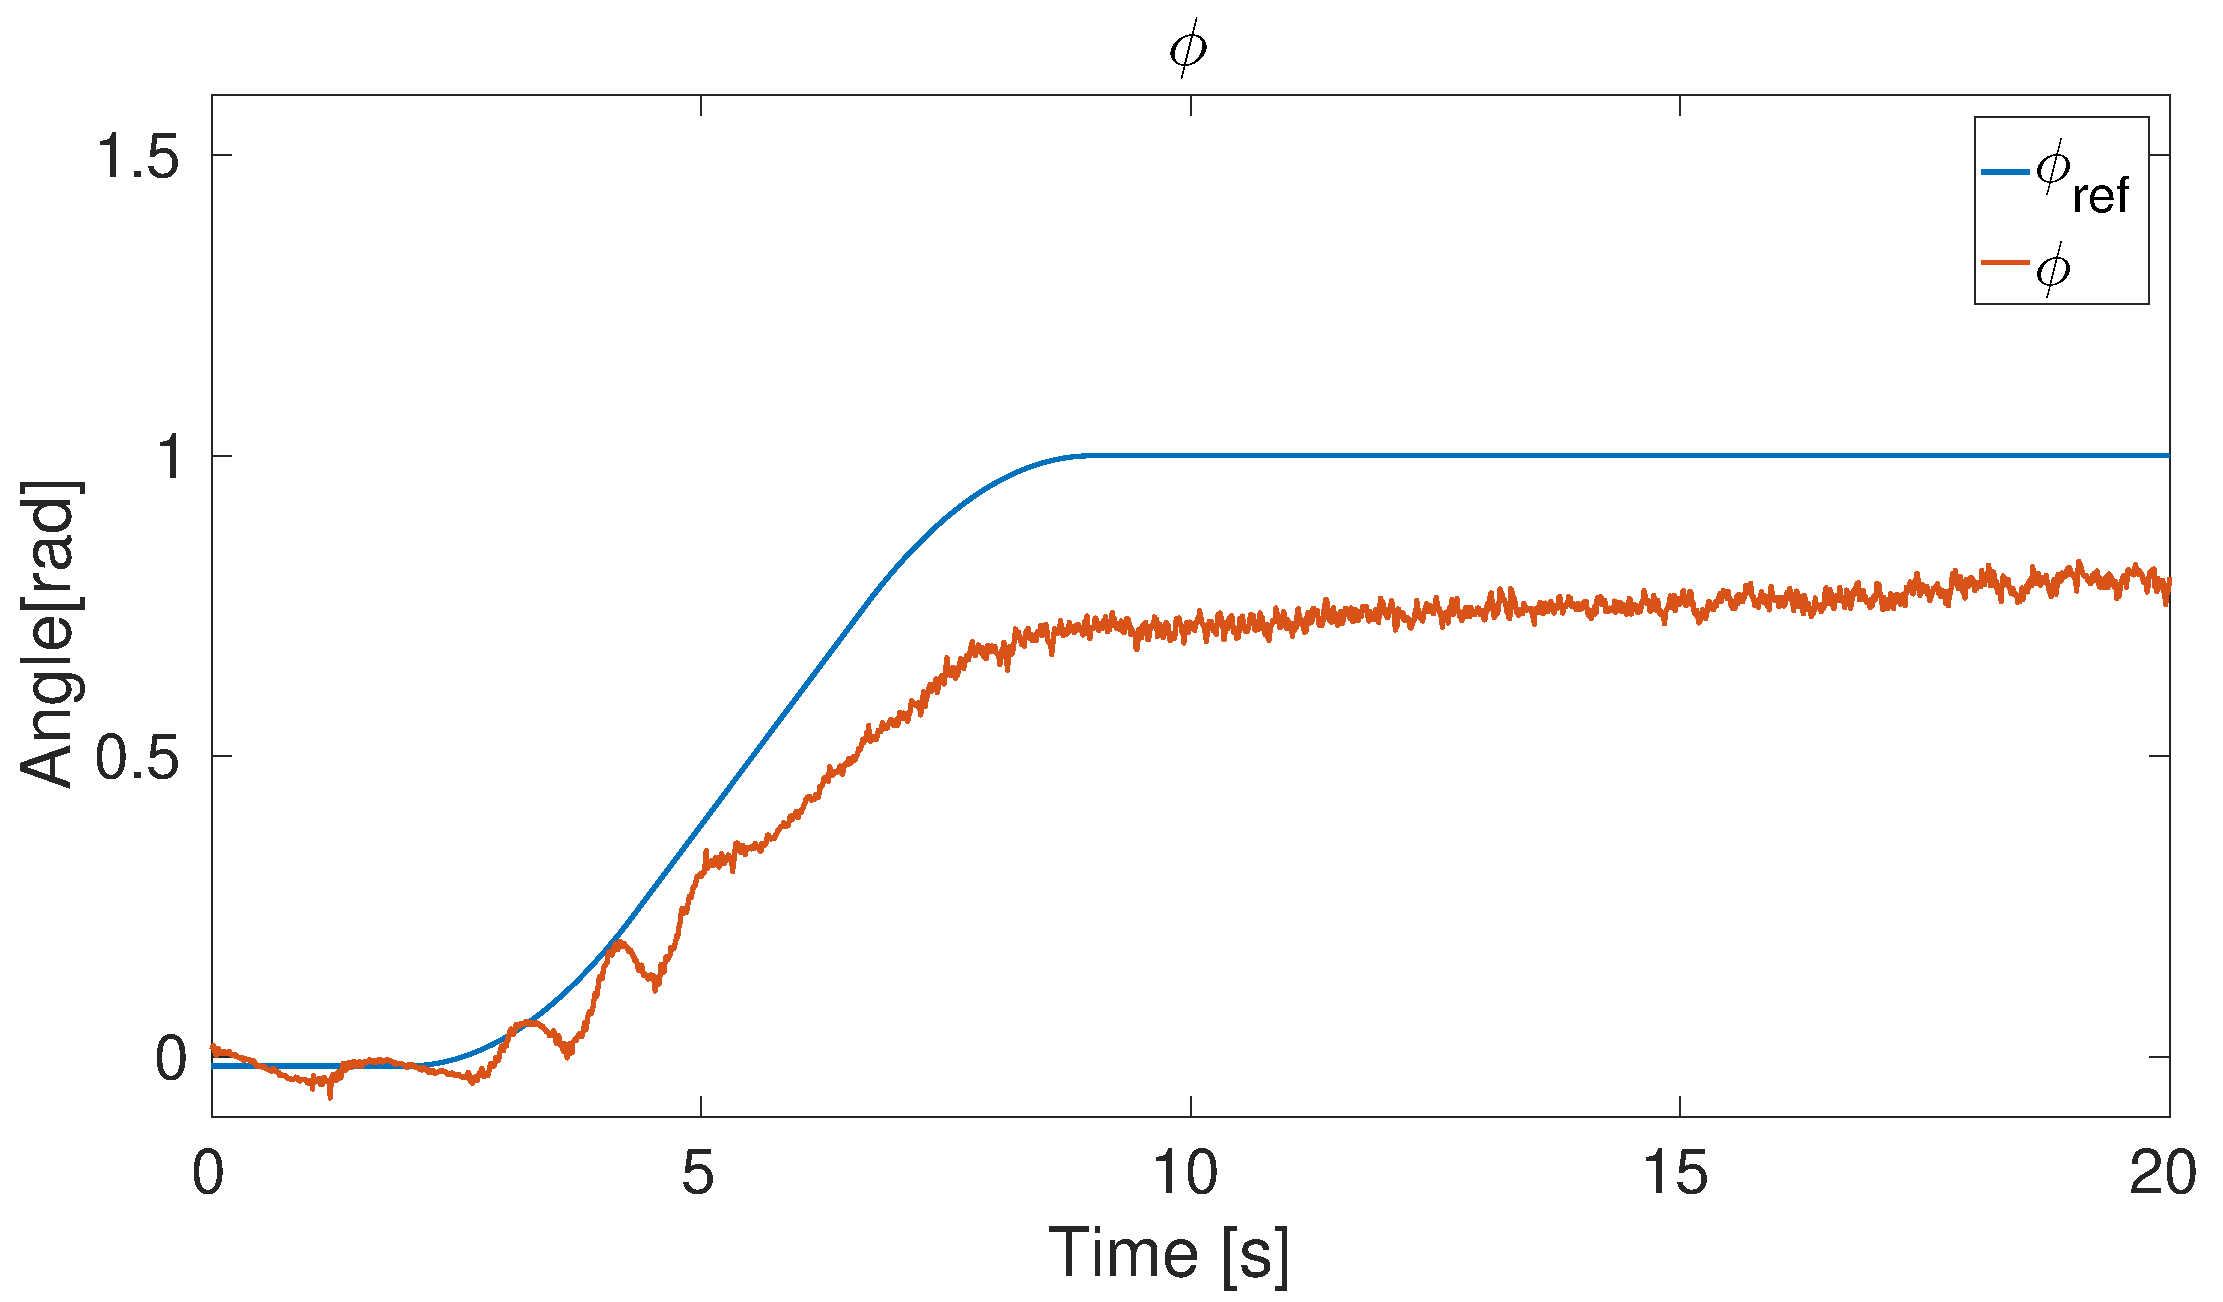
\includegraphics[width=0.4\textwidth]{testStepPhis3e10a1}}
  \qquad
  \subfloat[][\label{fig:AppsimStepRoll} Simulated response in $\rollAngle$.]{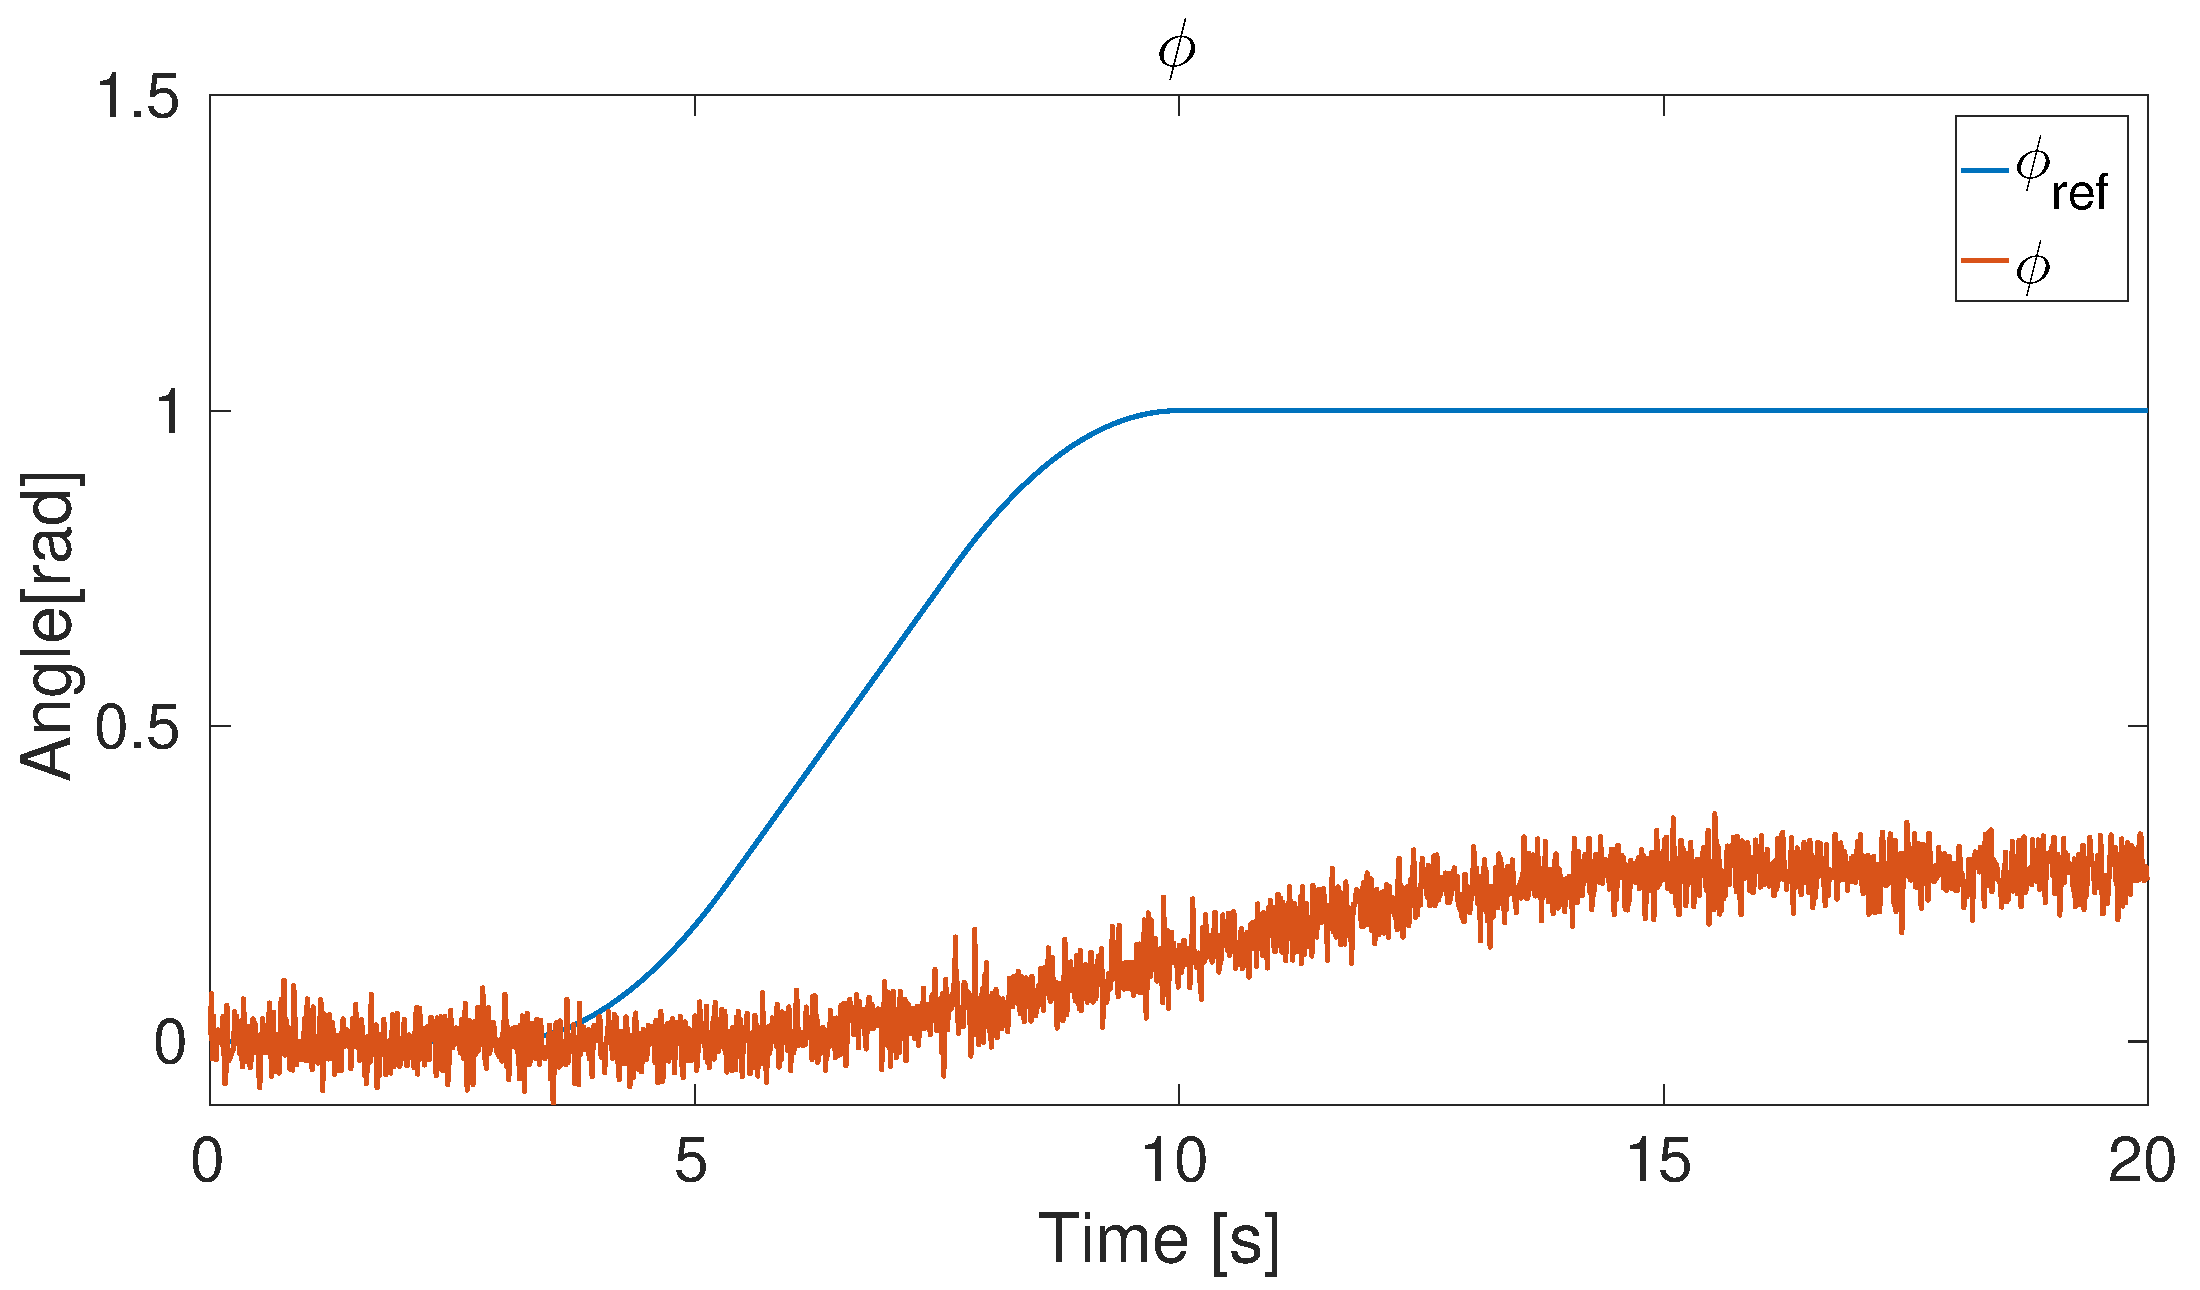
\includegraphics[width=0.4\textwidth]{simStepPhis3e10a1}}
  \qquad
  \subfloat[][\label{fig:ApptestStepPitch} Test response in $\pitchAngle$.]{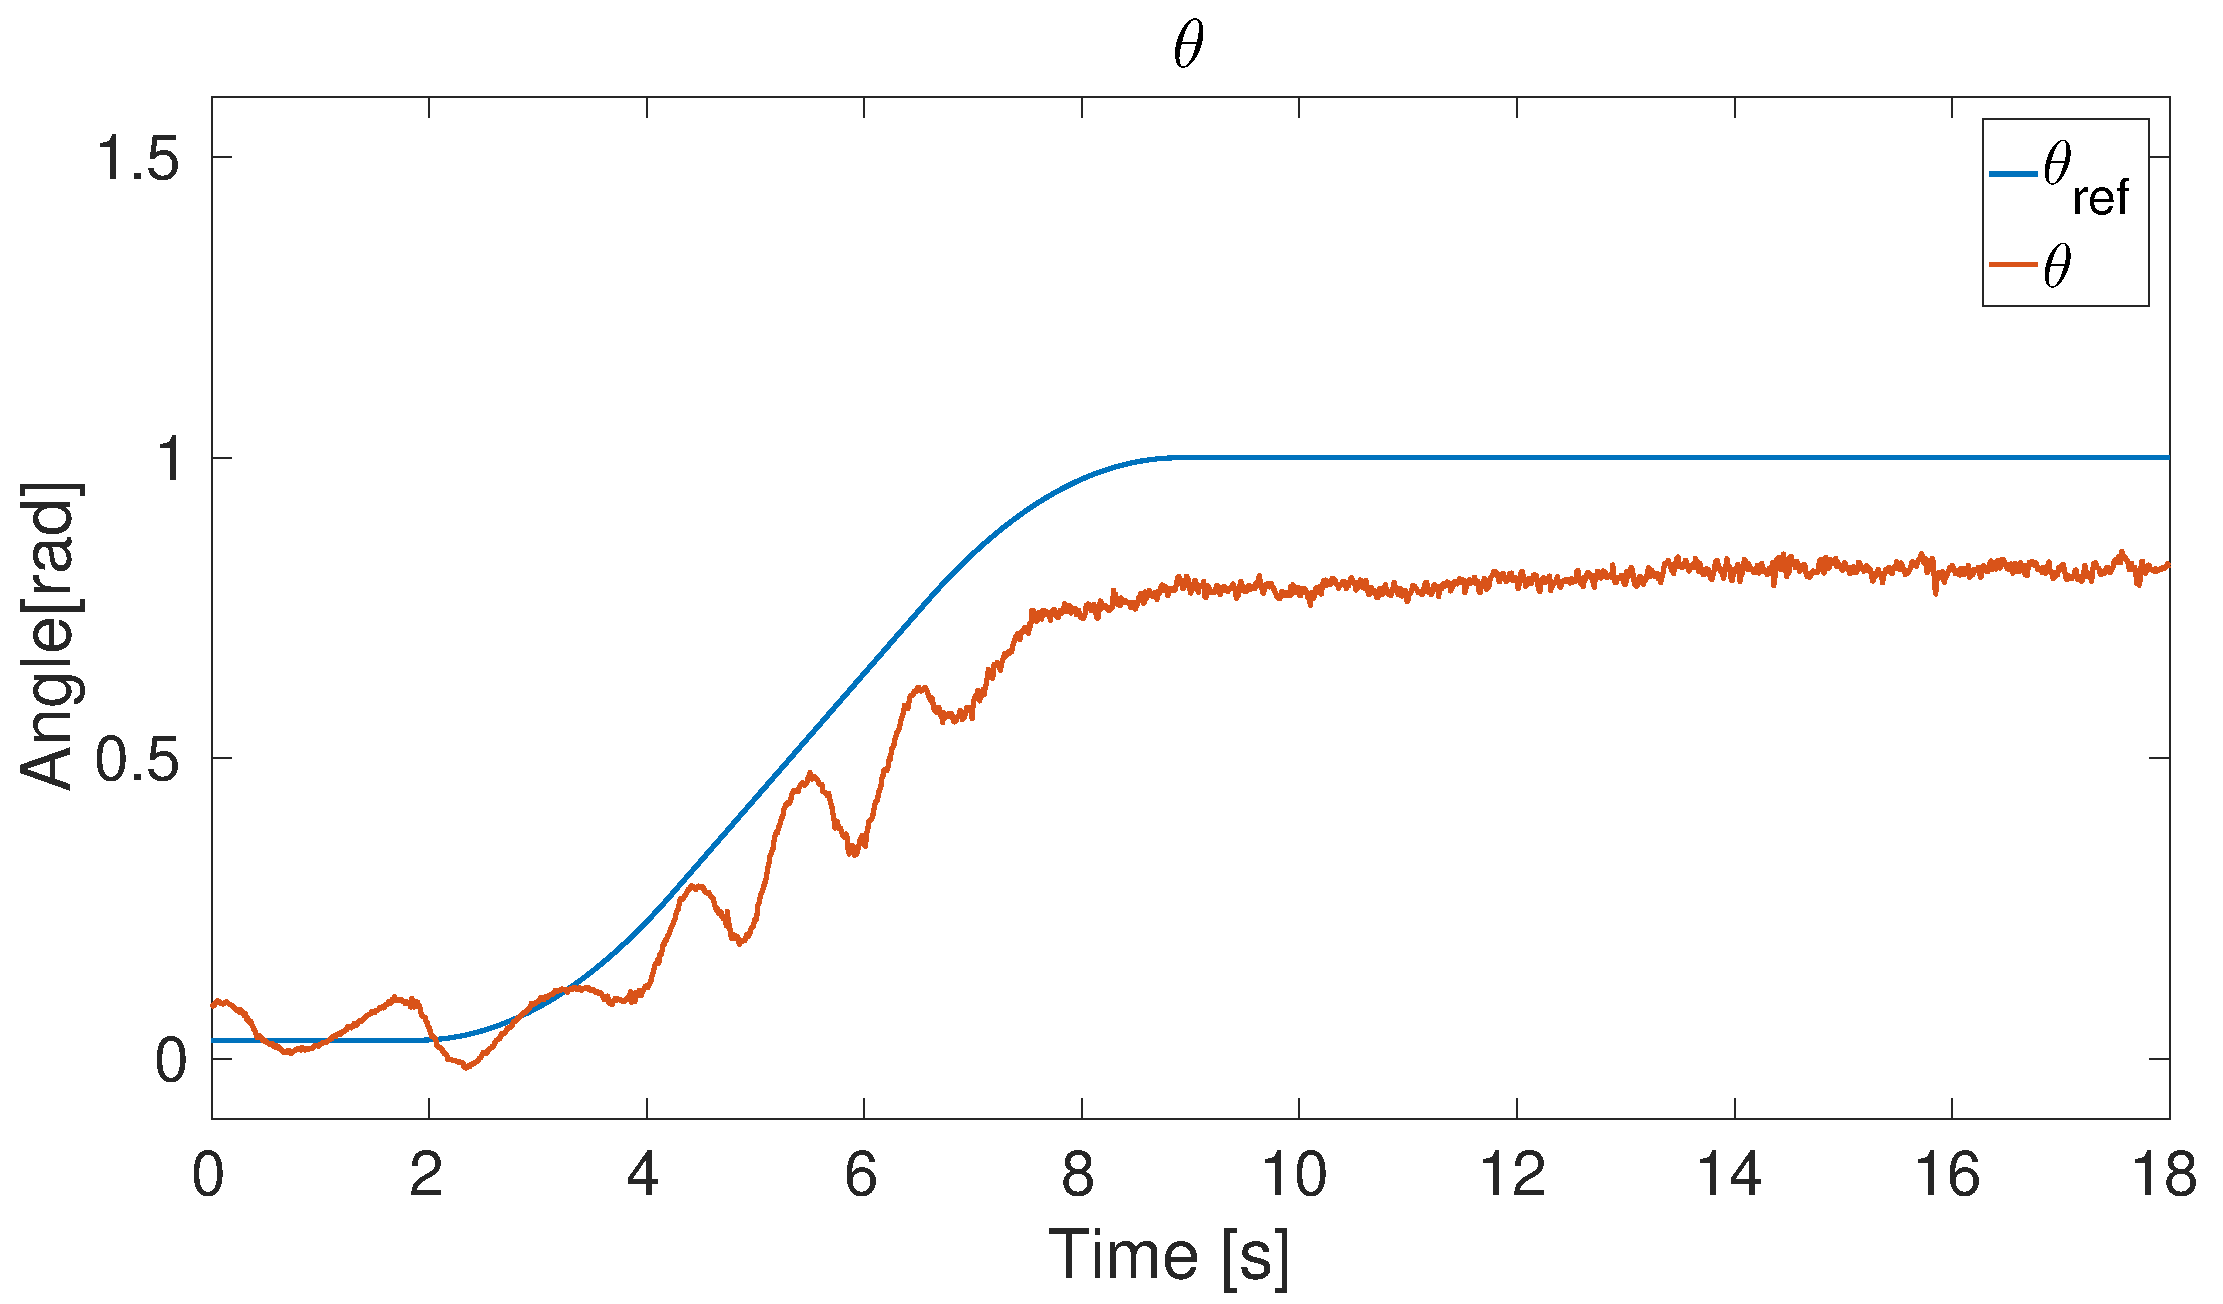
\includegraphics[width=0.4\textwidth]{testStepThetas3e10a1}}
  \qquad
  \subfloat[][\label{fig:AppsimStepPitch} Simulated response in $\pitchAngle$.]{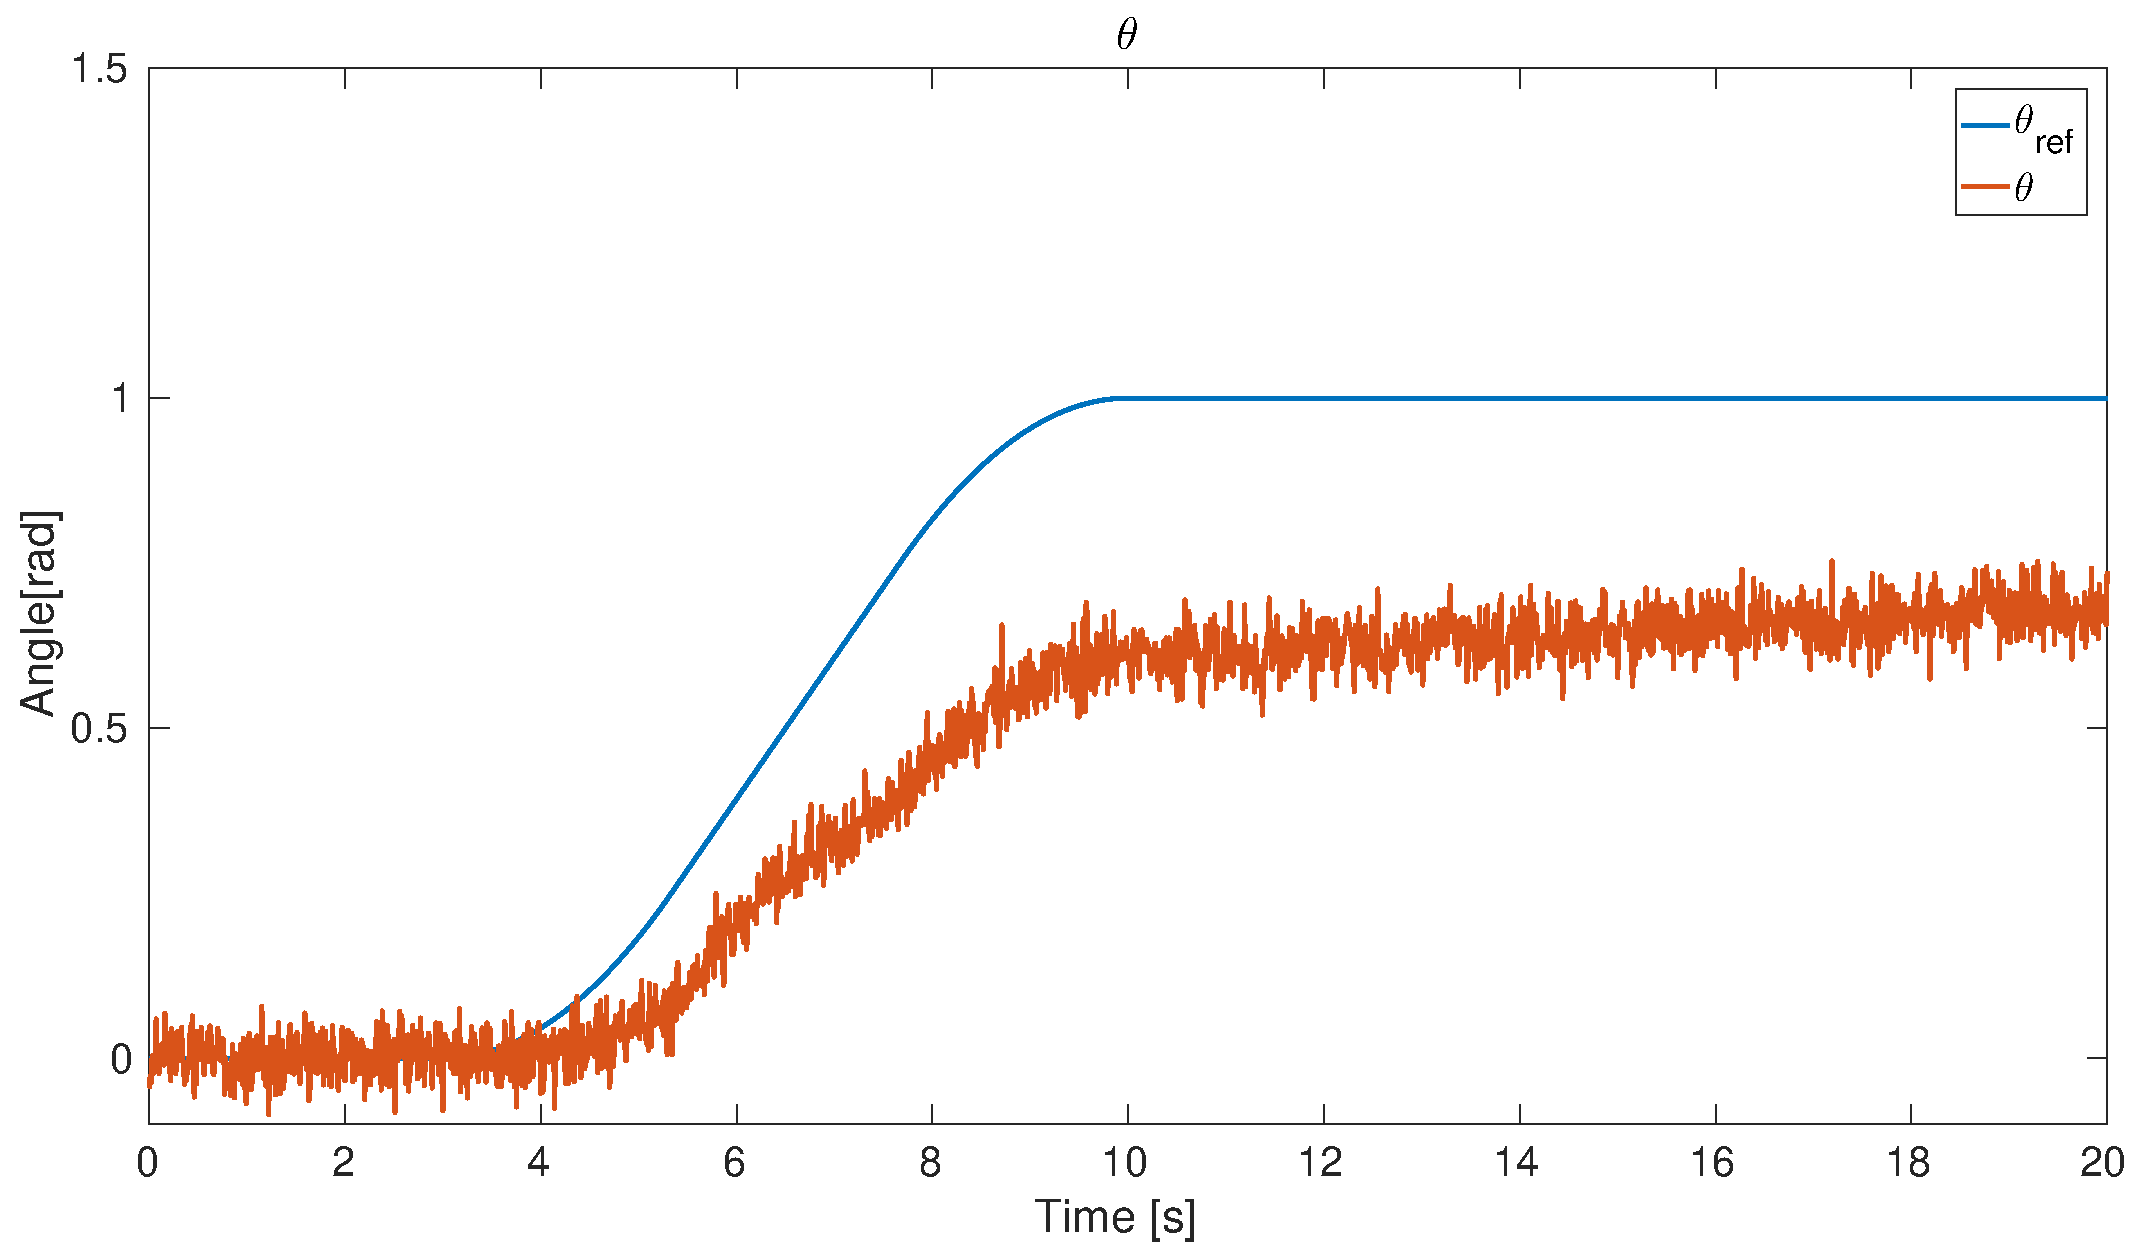
\includegraphics[width=0.4\textwidth]{simStepThetas3e10a1}}
  \qquad
  \subfloat[][\label{fig:ApptestStepYaw} Test response in $\yawAngle$.]{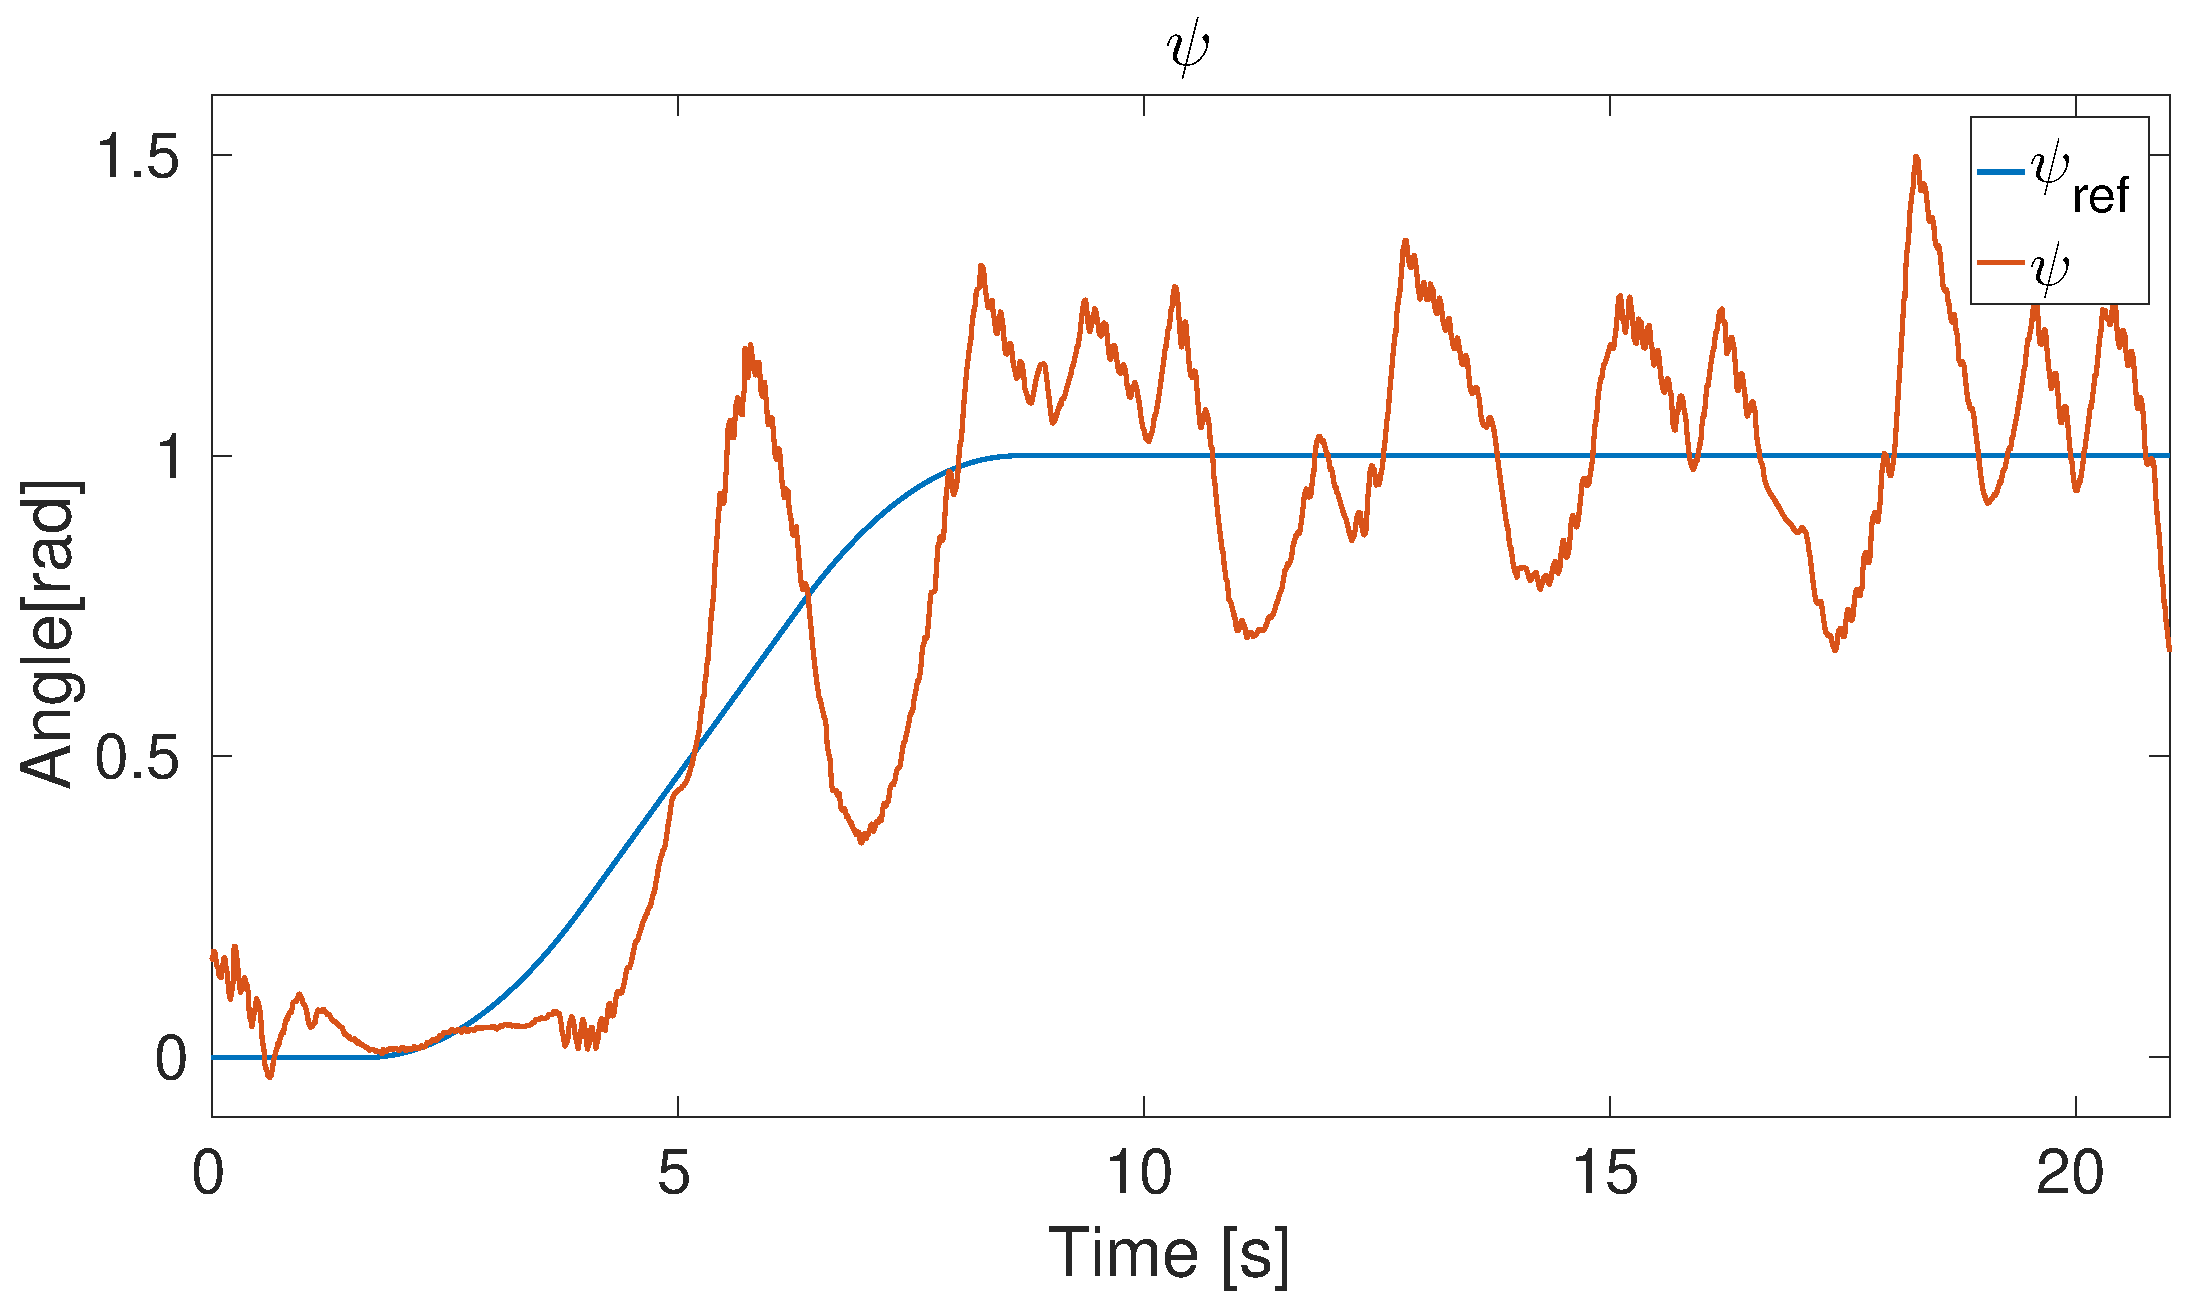
\includegraphics[width=0.4\textwidth]{testStepPsis3e10a1}}
  \qquad
  \subfloat[][\label{fig:AppsimStepYaw} Simulated response in $\yawAngle$.]{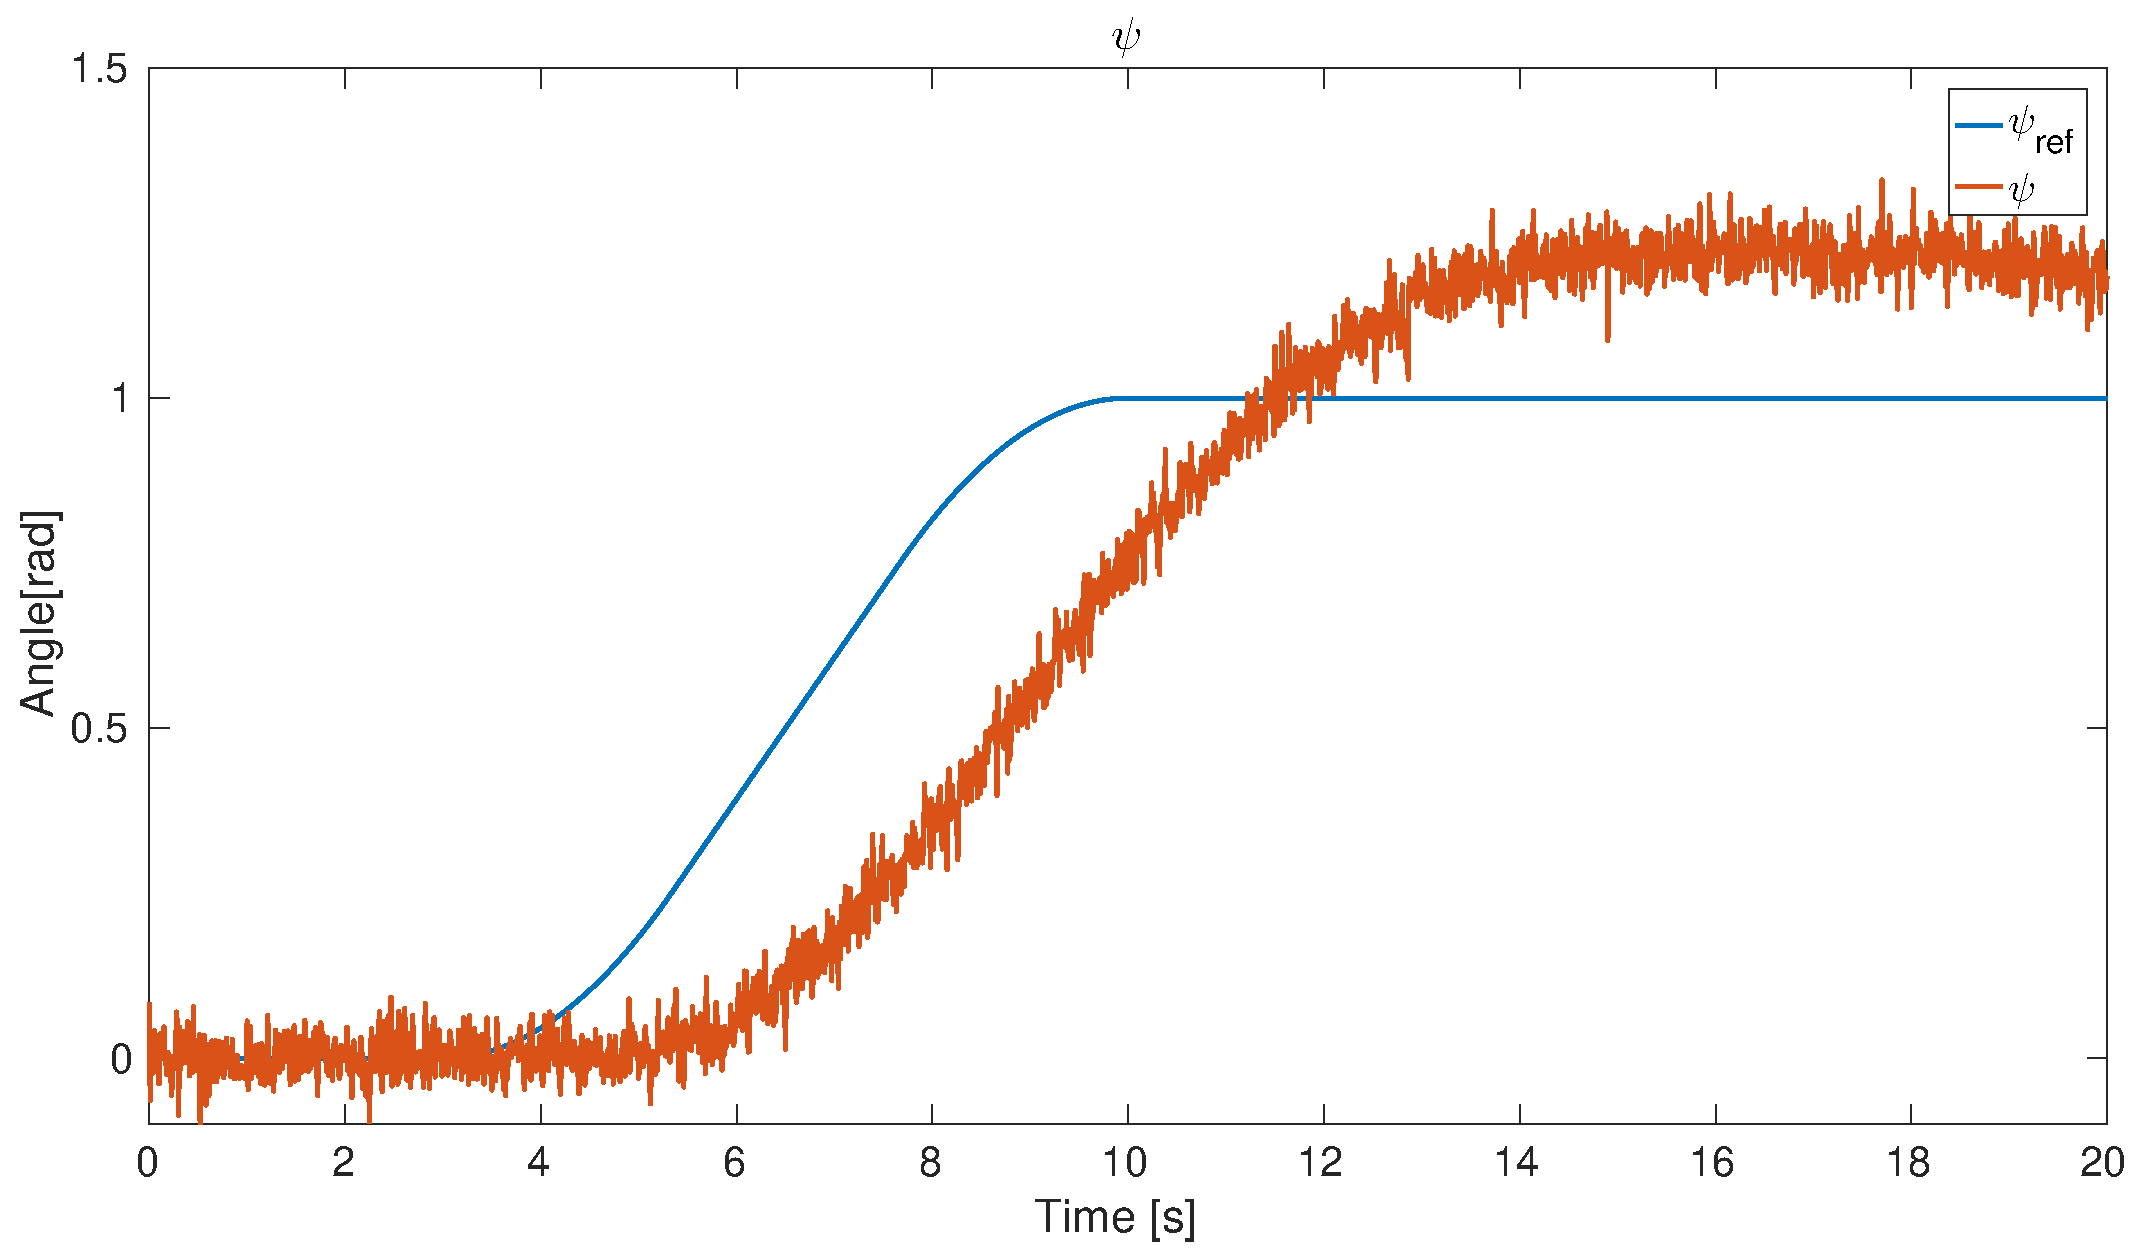
\includegraphics[width=0.4\textwidth]{simStepPsis3e10a1}}
   \caption{\label{fig:AppStepAttitude}%
   A smooth step with $q_{\text{0}} = 0$, $q_{\text{f}} = 1$, $t_{\text{s}} = 3$, $t_{\text{f}} = 15$ and $V = 1.5 (q_{\text{f}} - q_{\text{0}})/(t_{\text{f}} - t_{\text{s}}))$ was applied in one attitude angle at a time while using the attitude controller. While a smooth step was applied in one attitude angle the other attitude angles were not controlled.}
\end{figure}

\begin{figure}
\centering
  \subfloat[][\label{fig:ApptestStepAllRollAttitude} Test response in $\rollAngle$.]{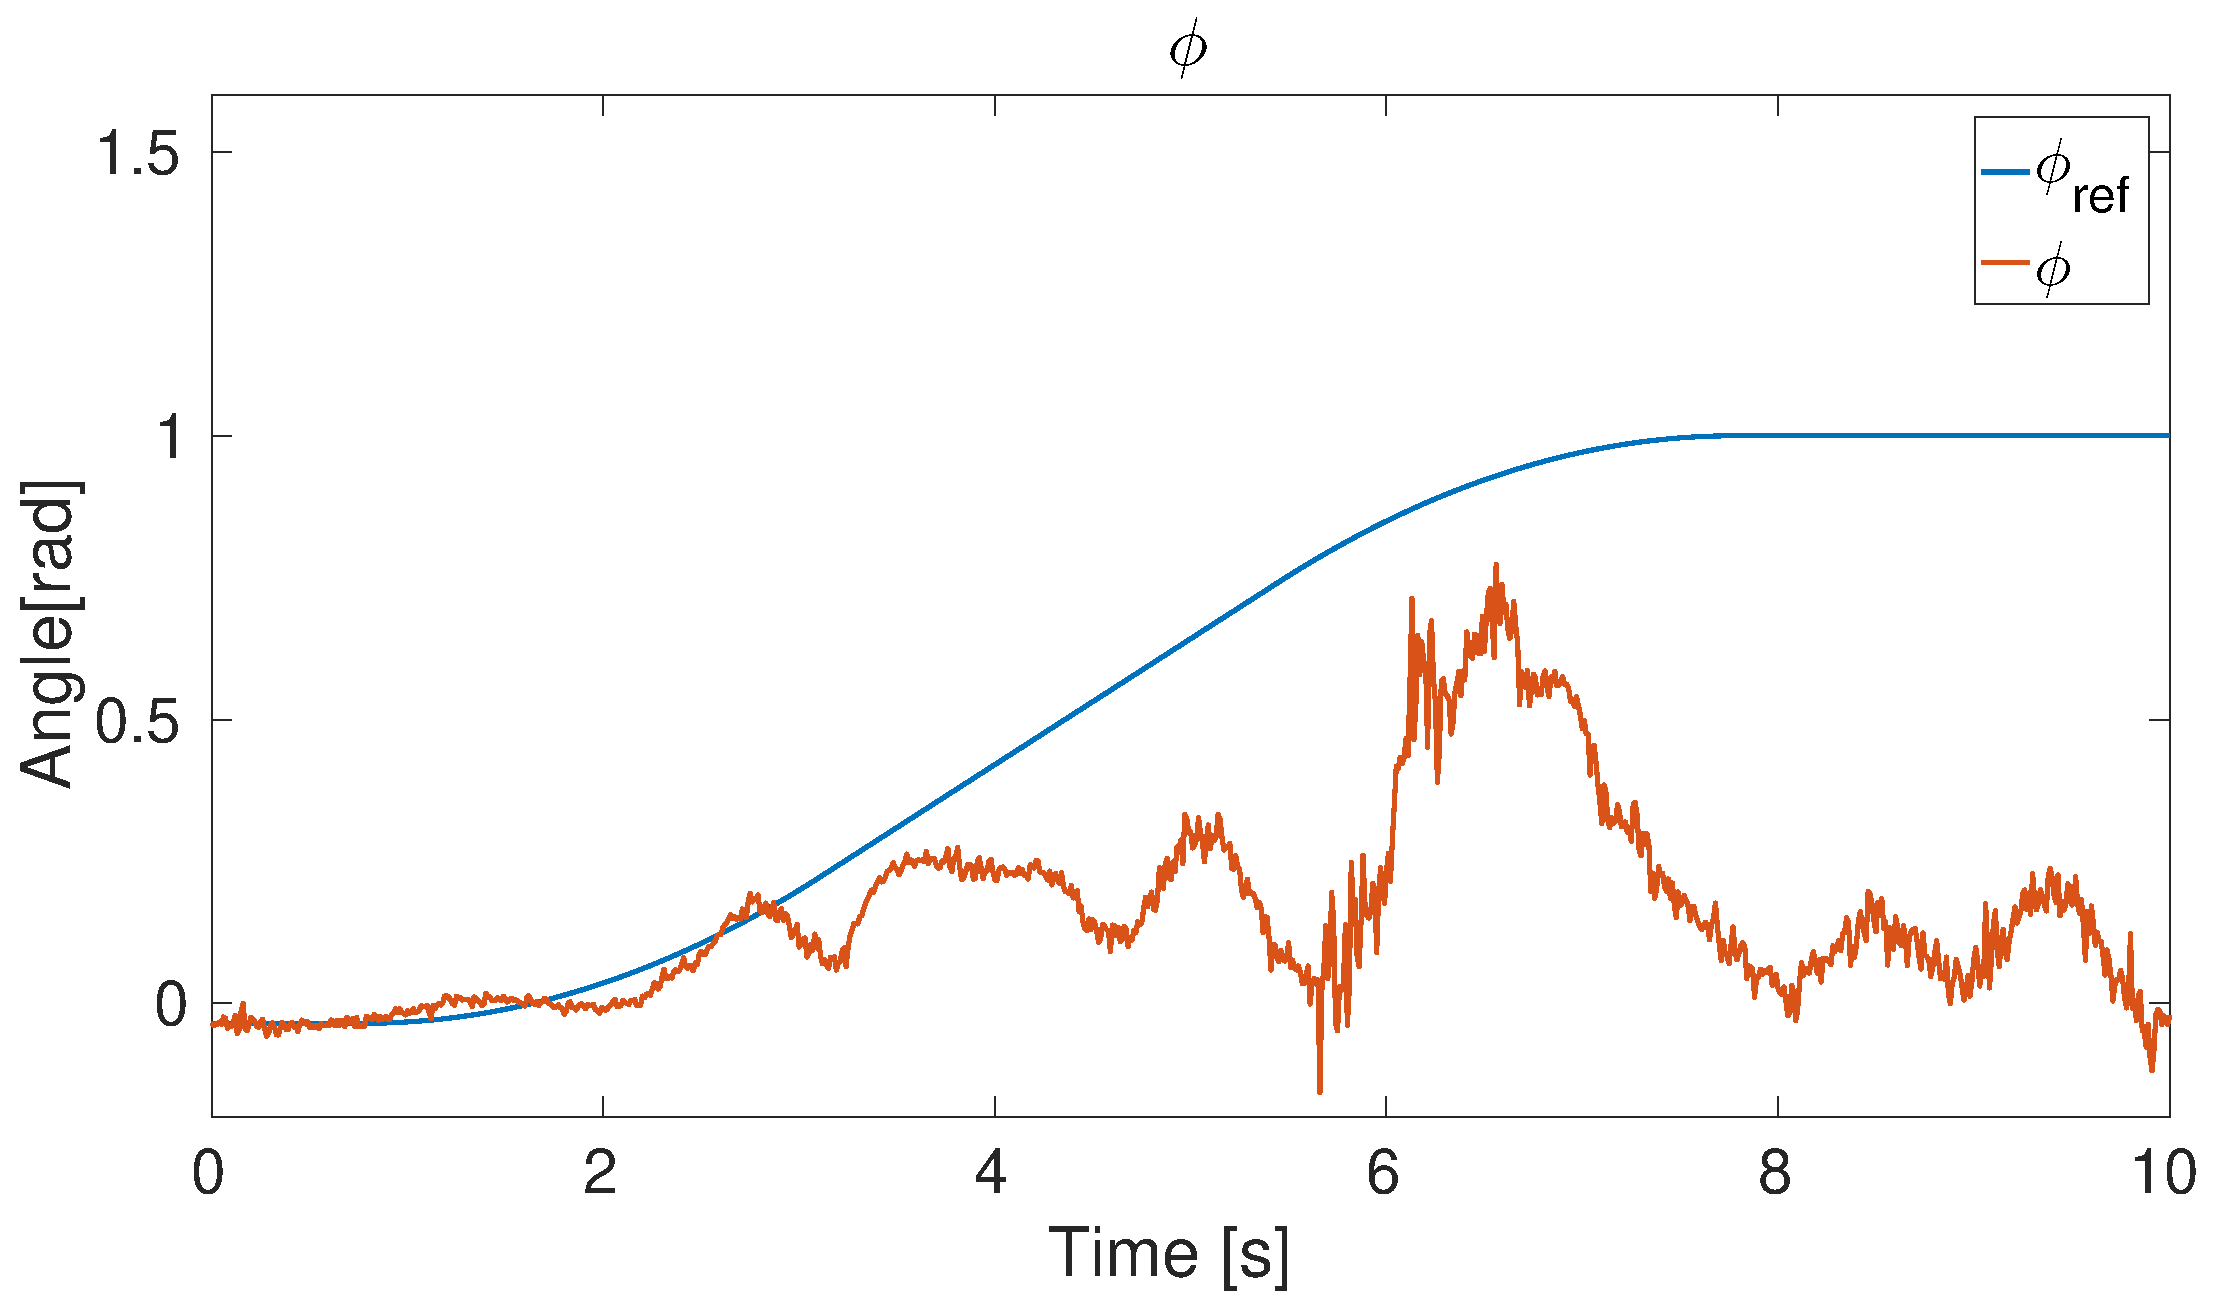
\includegraphics[width=0.4\textwidth]{testStepAllPhis3e10a1}}
  \qquad
  \subfloat[][\label{fig:AppsimStepAllRollAttitude} Simulated response in $\rollAngle$.]{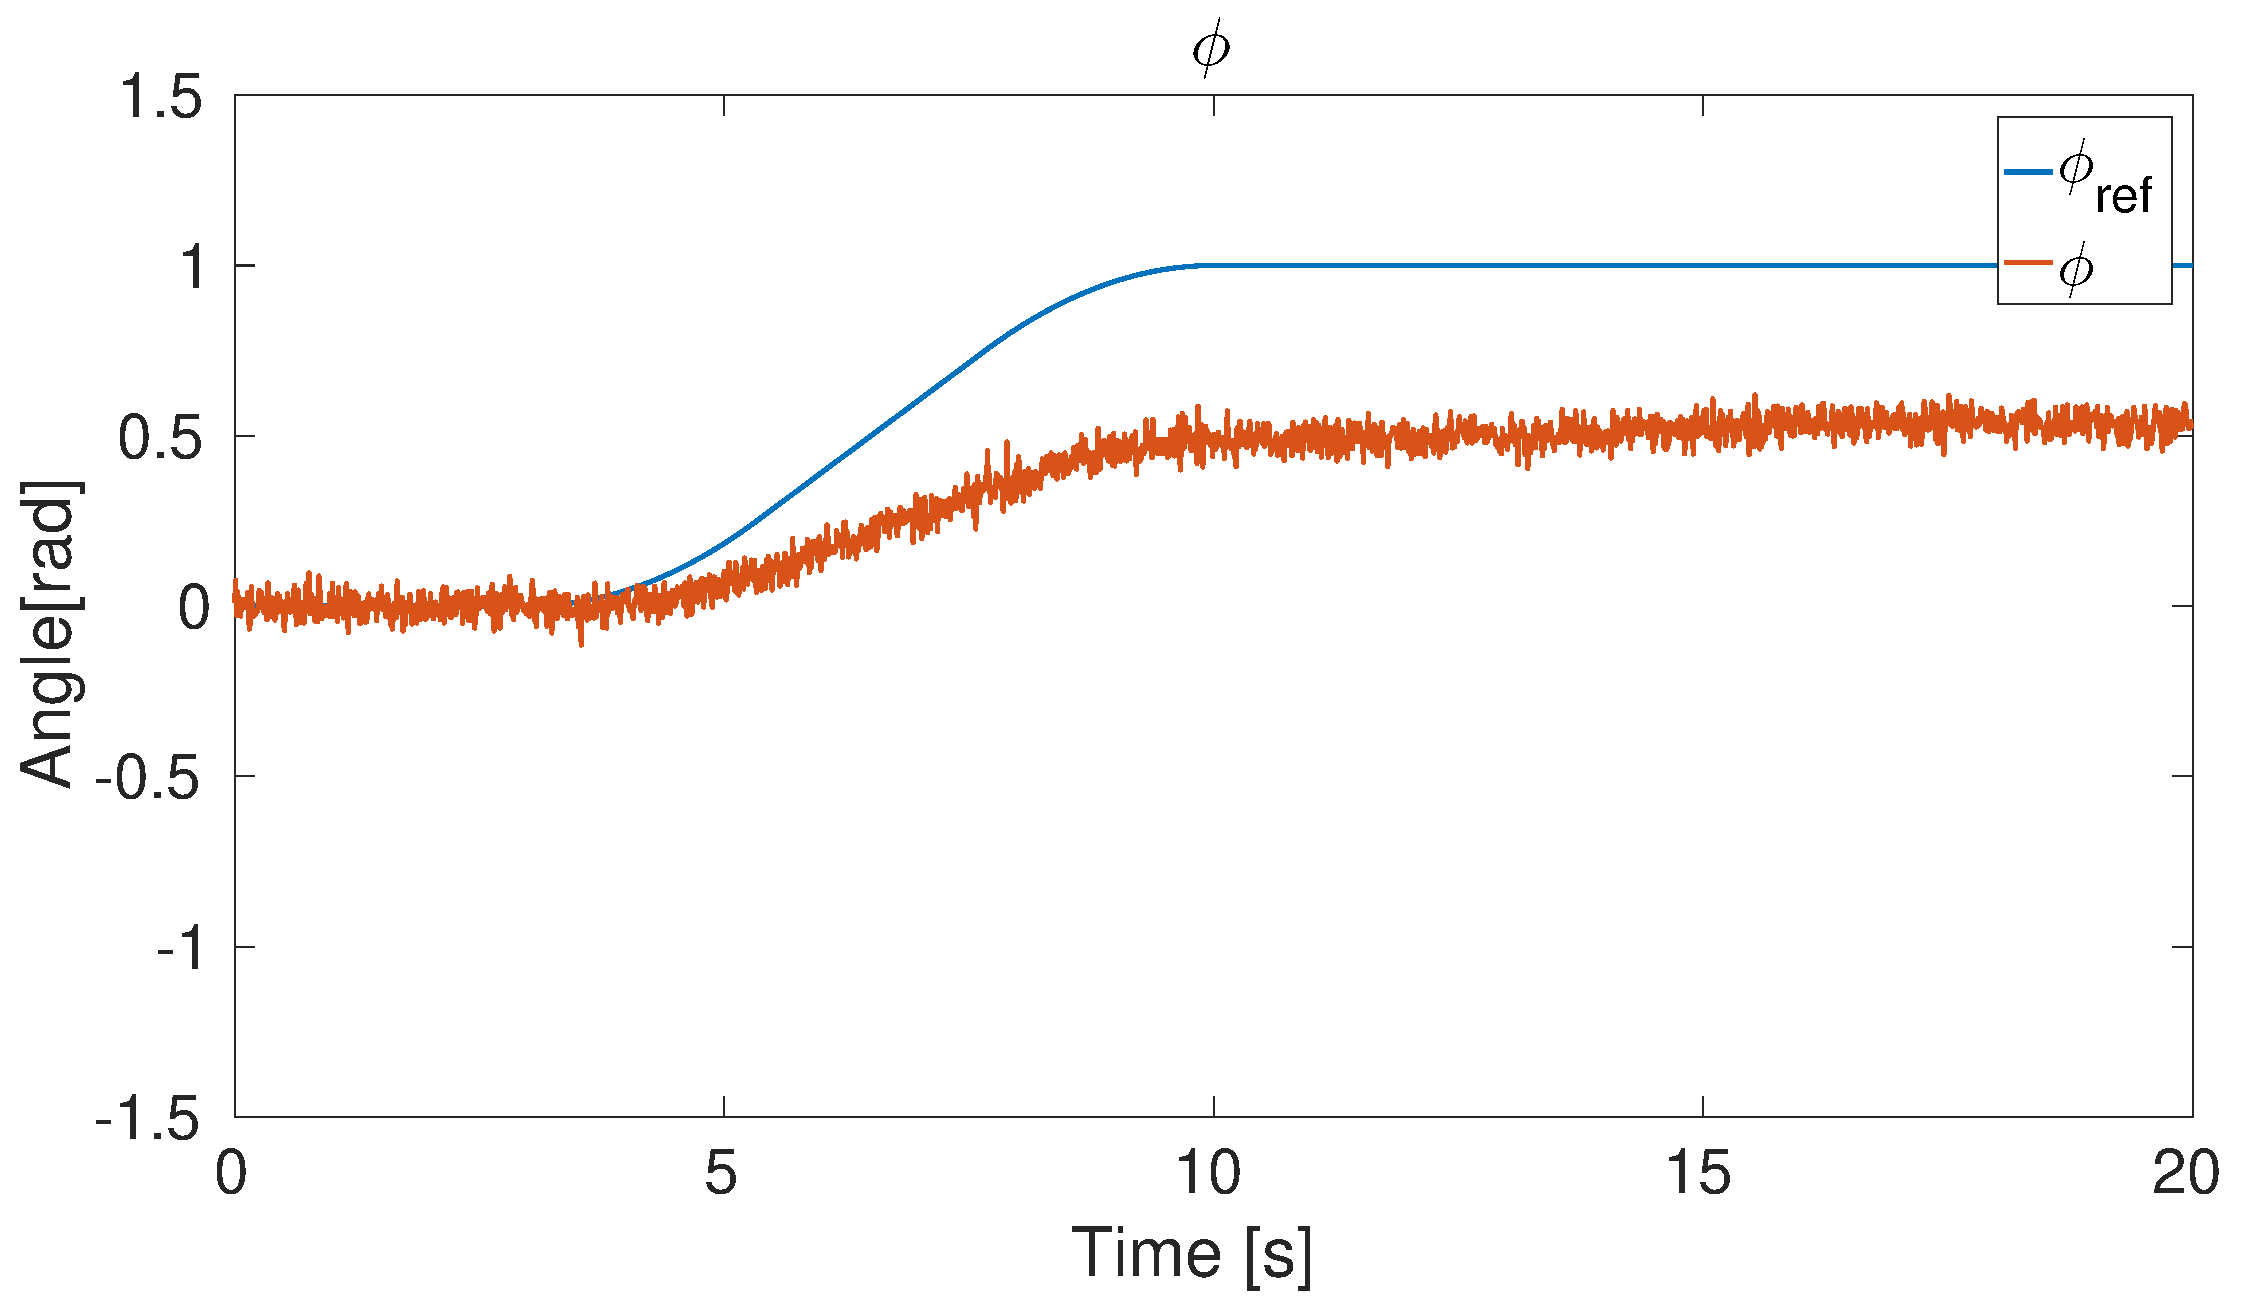
\includegraphics[width=0.4\textwidth]{simStepAllPhis3e10a1}}
  \qquad
  \subfloat[][\label{fig:AppTestStepAllPitchAttitude} Test response in $\pitchAngle$.]{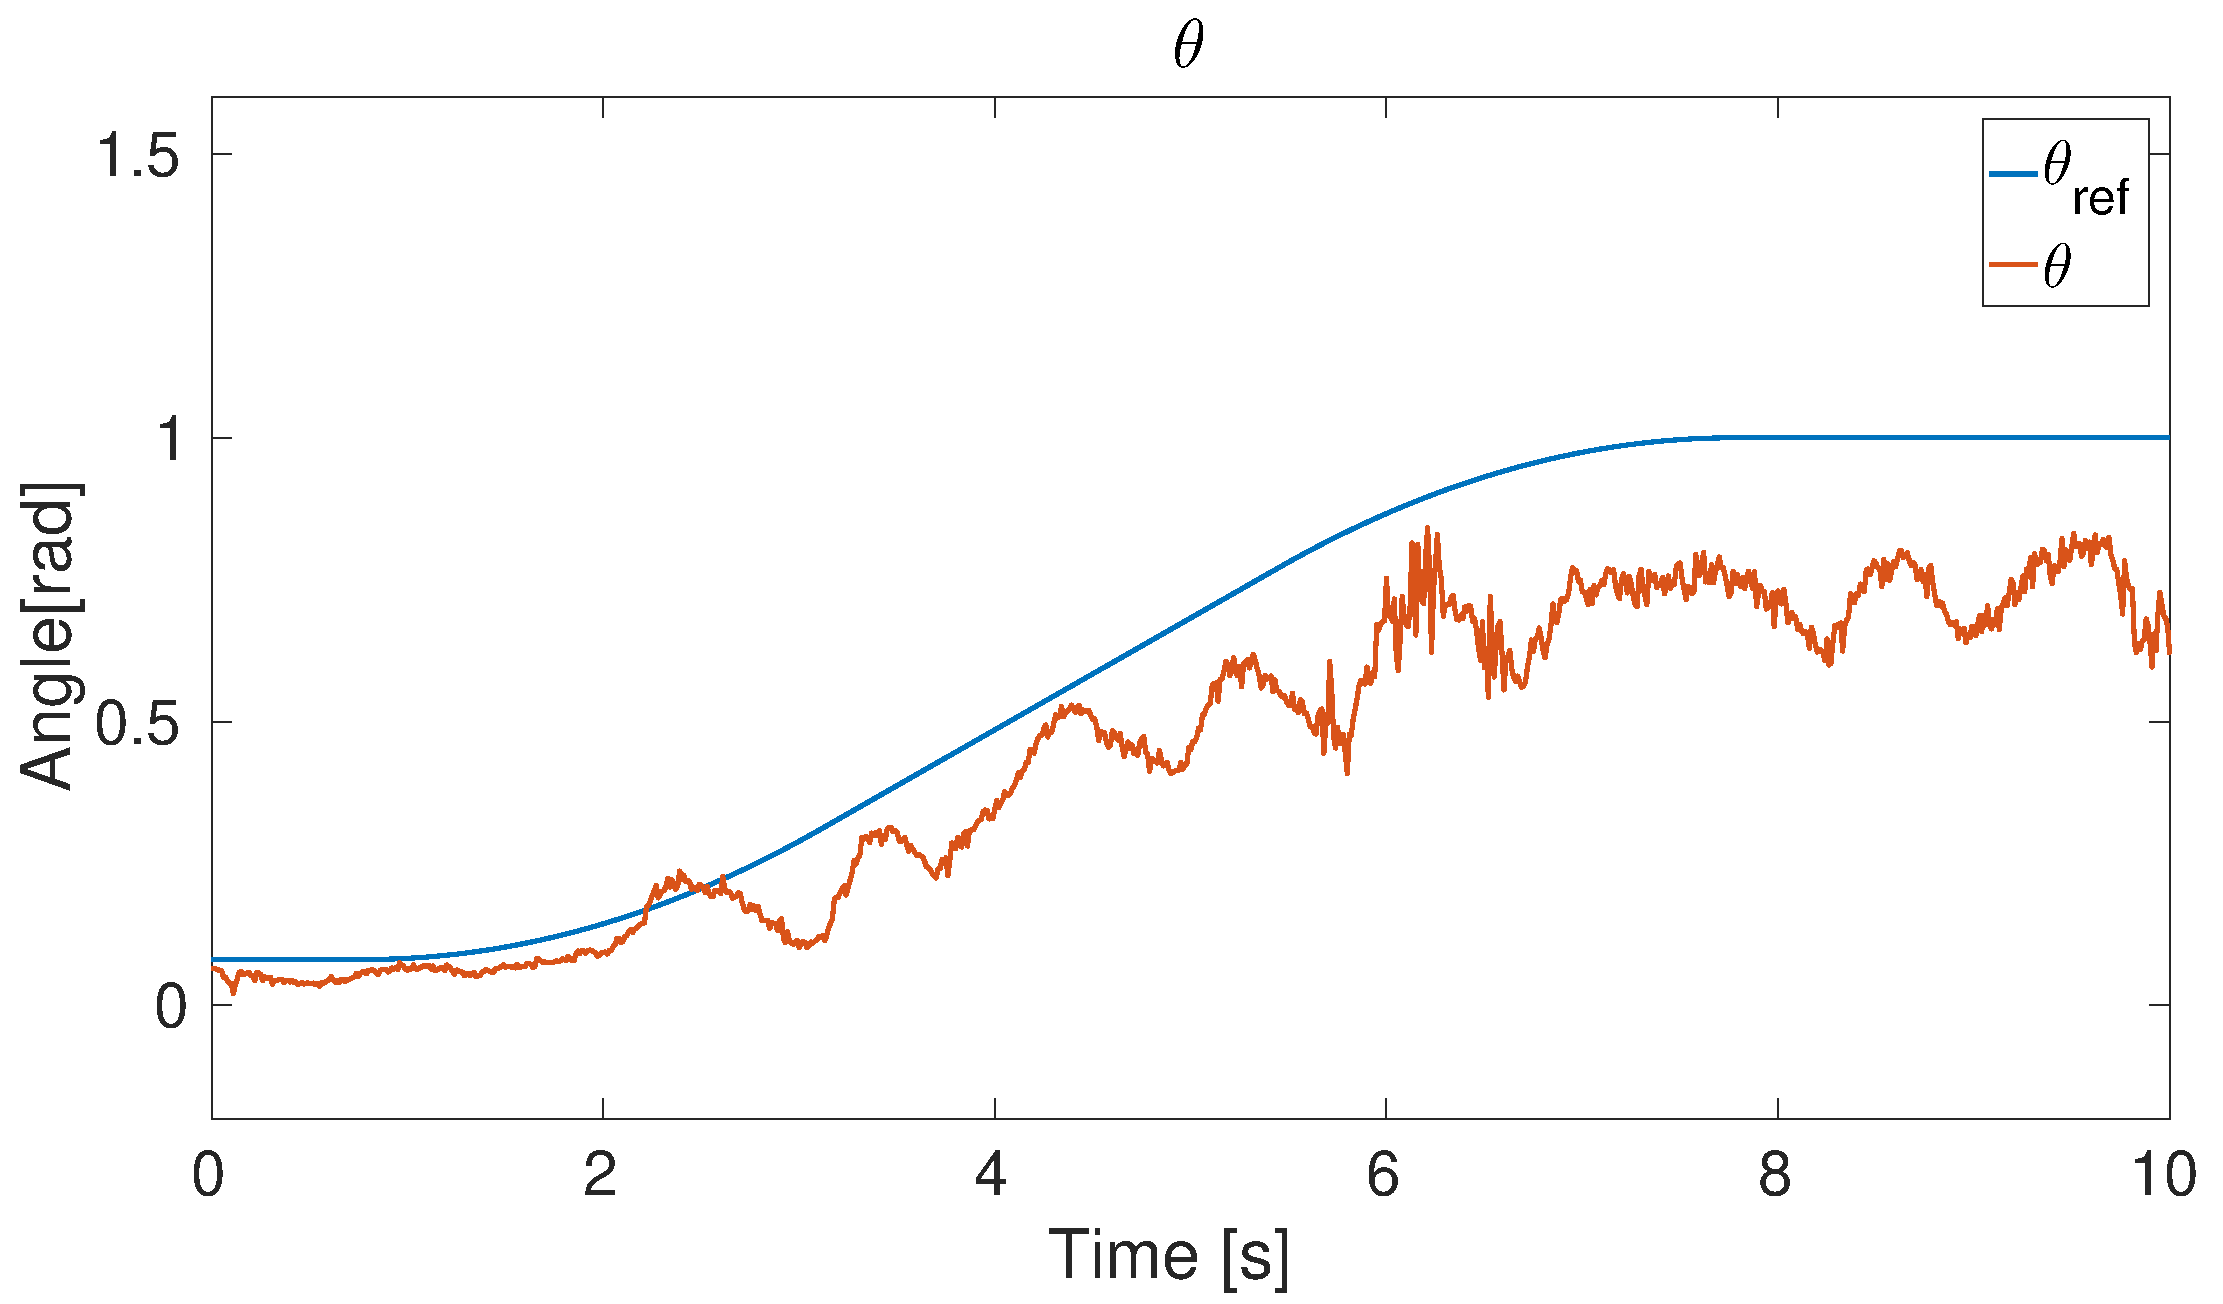
\includegraphics[width=0.4\textwidth]{testStepAllThetas3e10a1}}
  \qquad
  \subfloat[][\label{fig:AppsimStepAllPitchAttitude} Simulated response in $\pitchAngle$.]{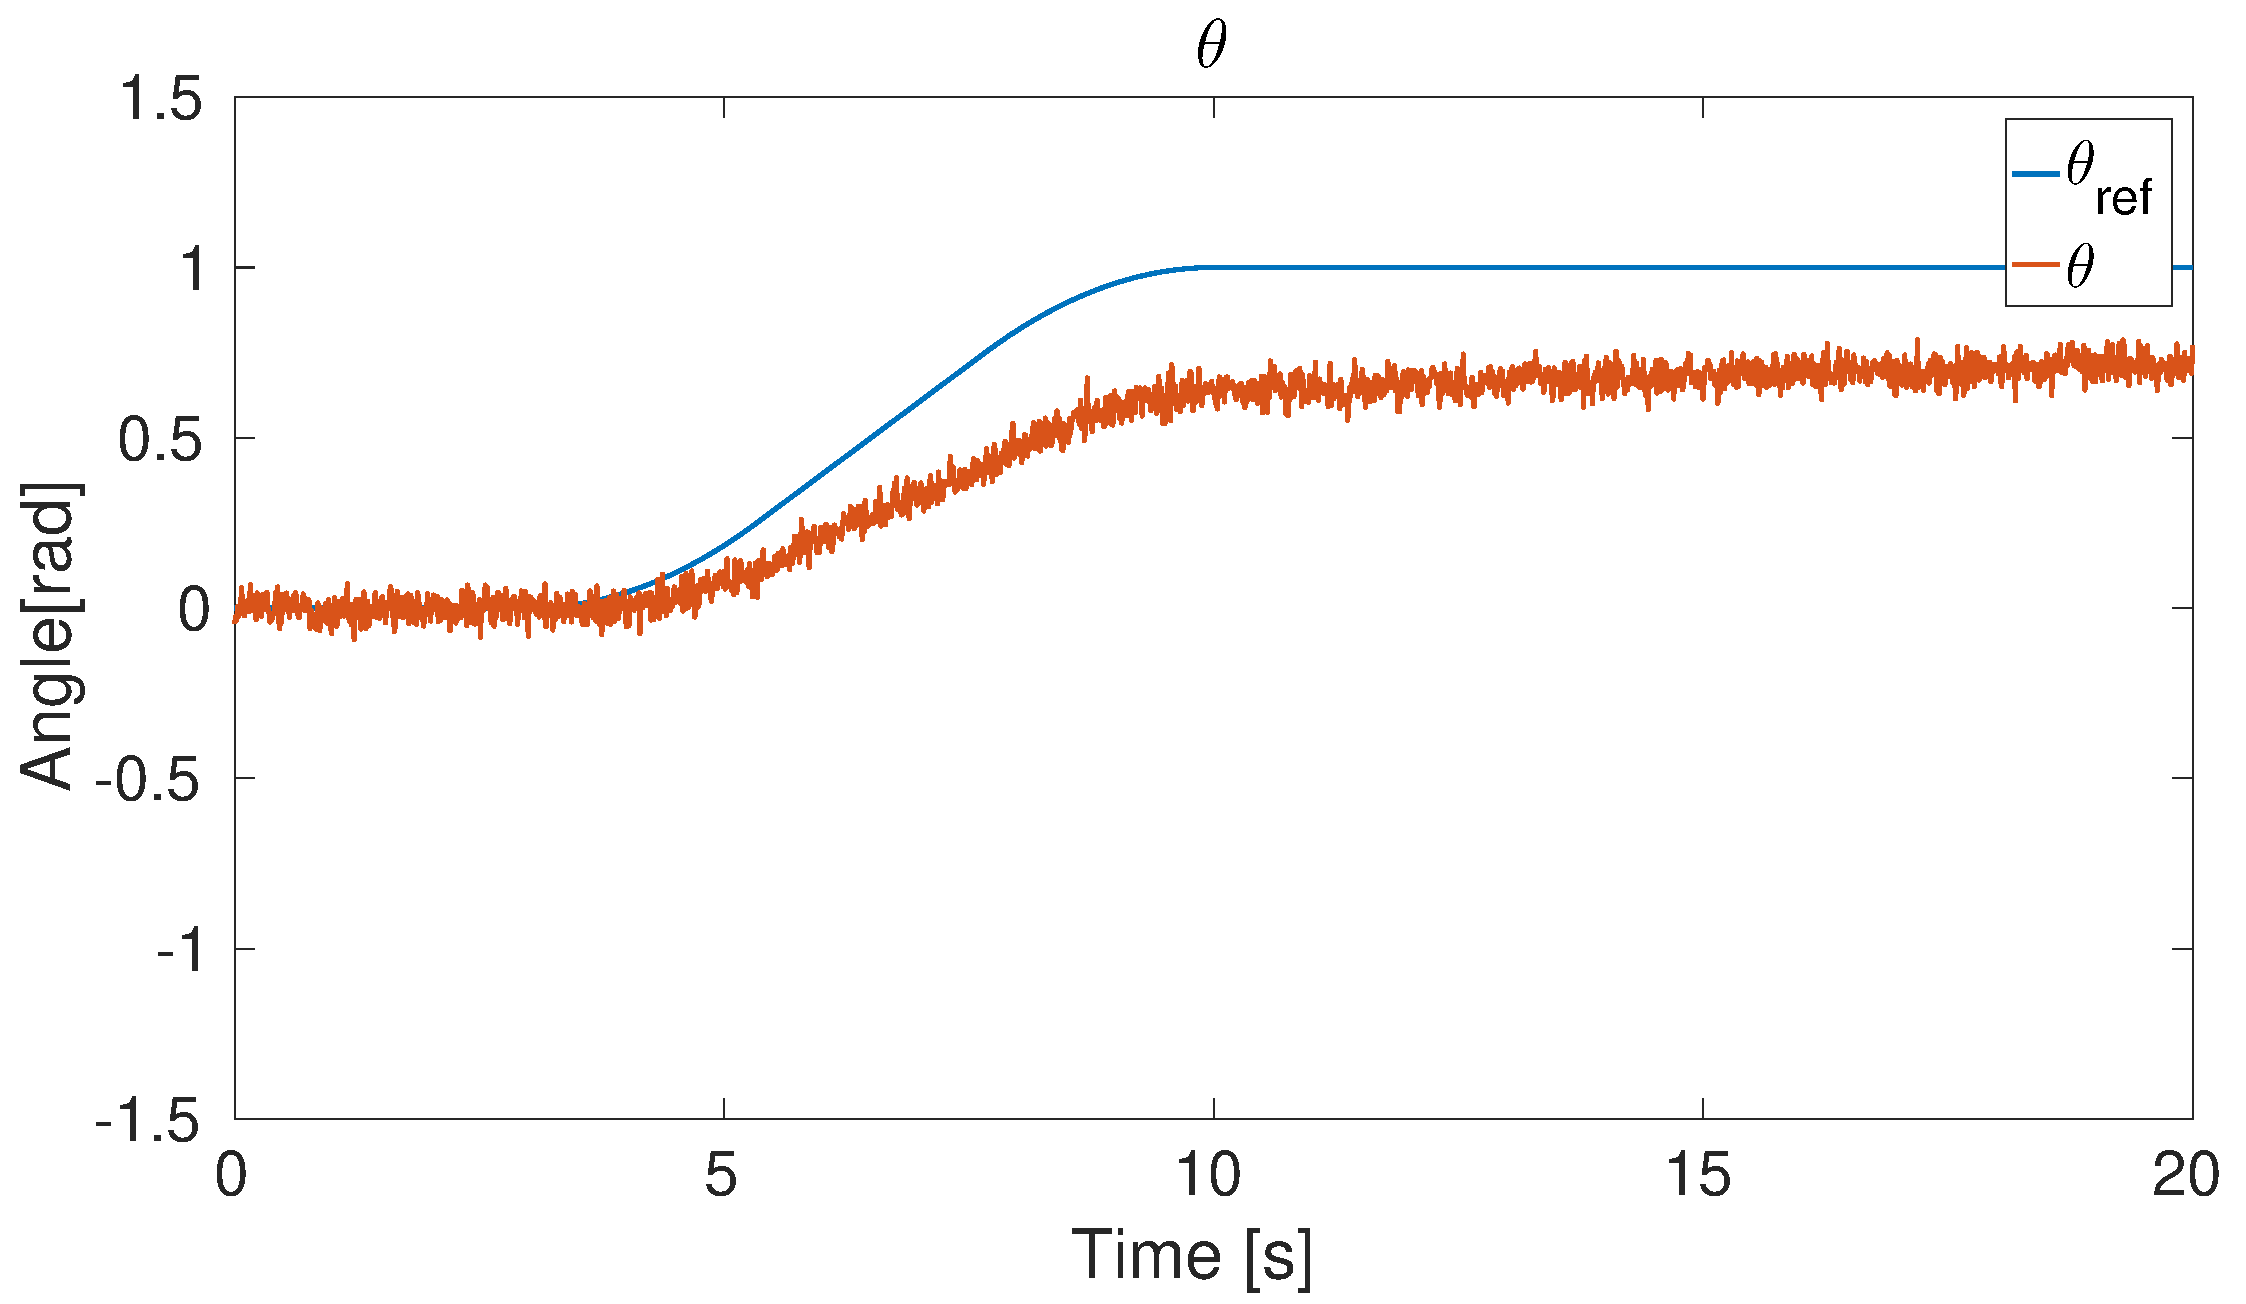
\includegraphics[width=0.4\textwidth]{simStepAllThetas3e10a1}}
  \qquad
  \subfloat[][\label{fig:AppTestStepAllYawAttitude} Test response in $\yawAngle$.]{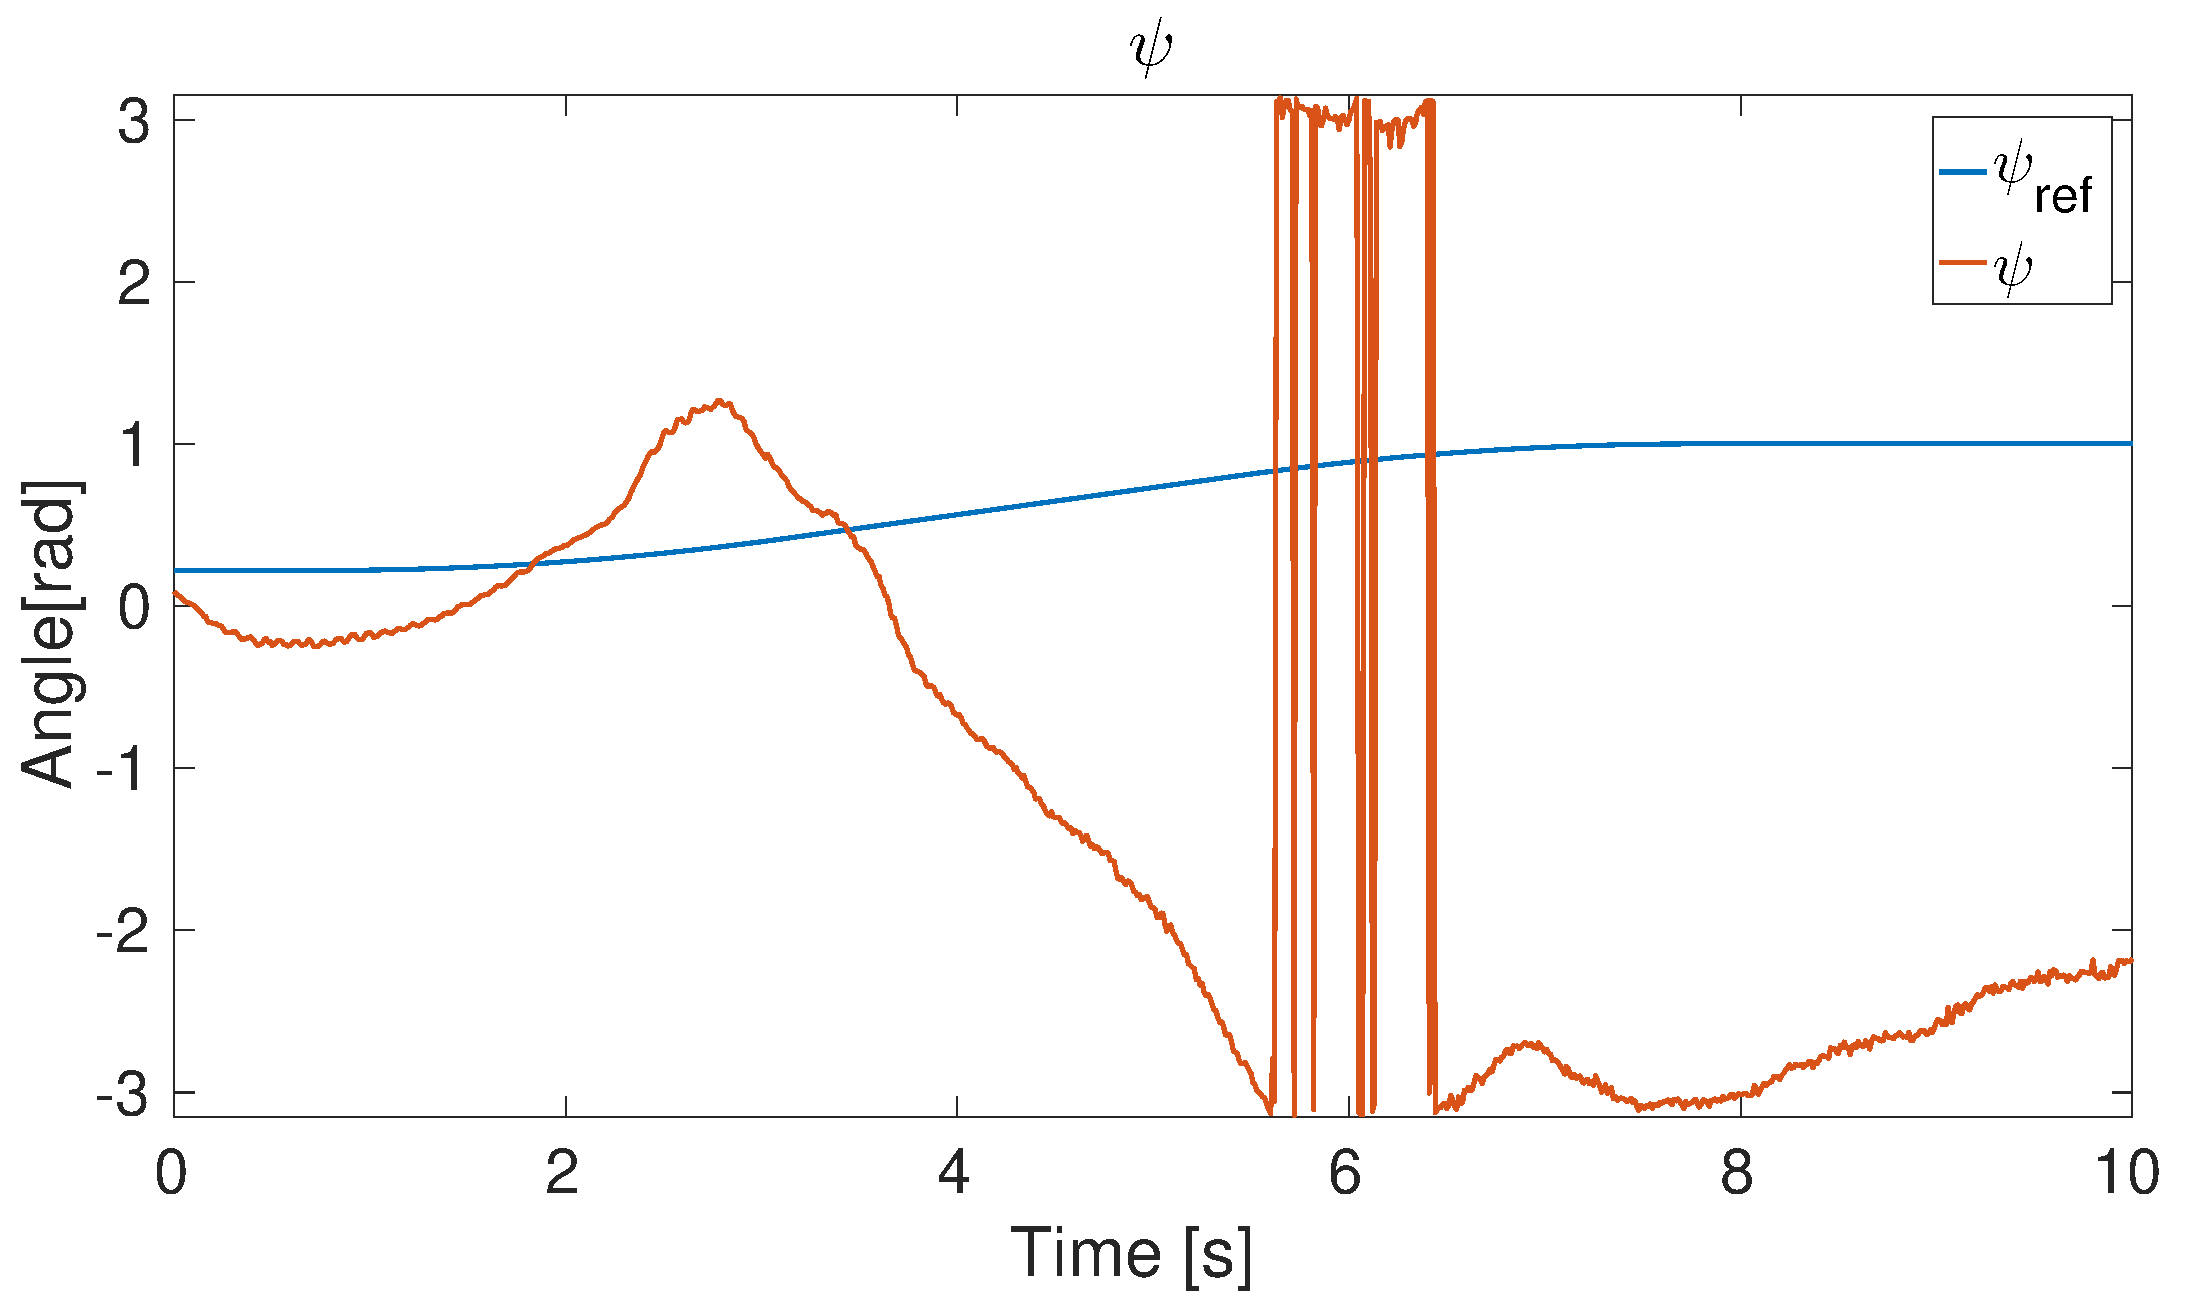
\includegraphics[width=0.4\textwidth]{testStepAllPsis3e10a1}}
  \qquad
  \subfloat[][\label{fig:AppsimStepAllYawAttitude} Simulated response in $\yawAngle$.]{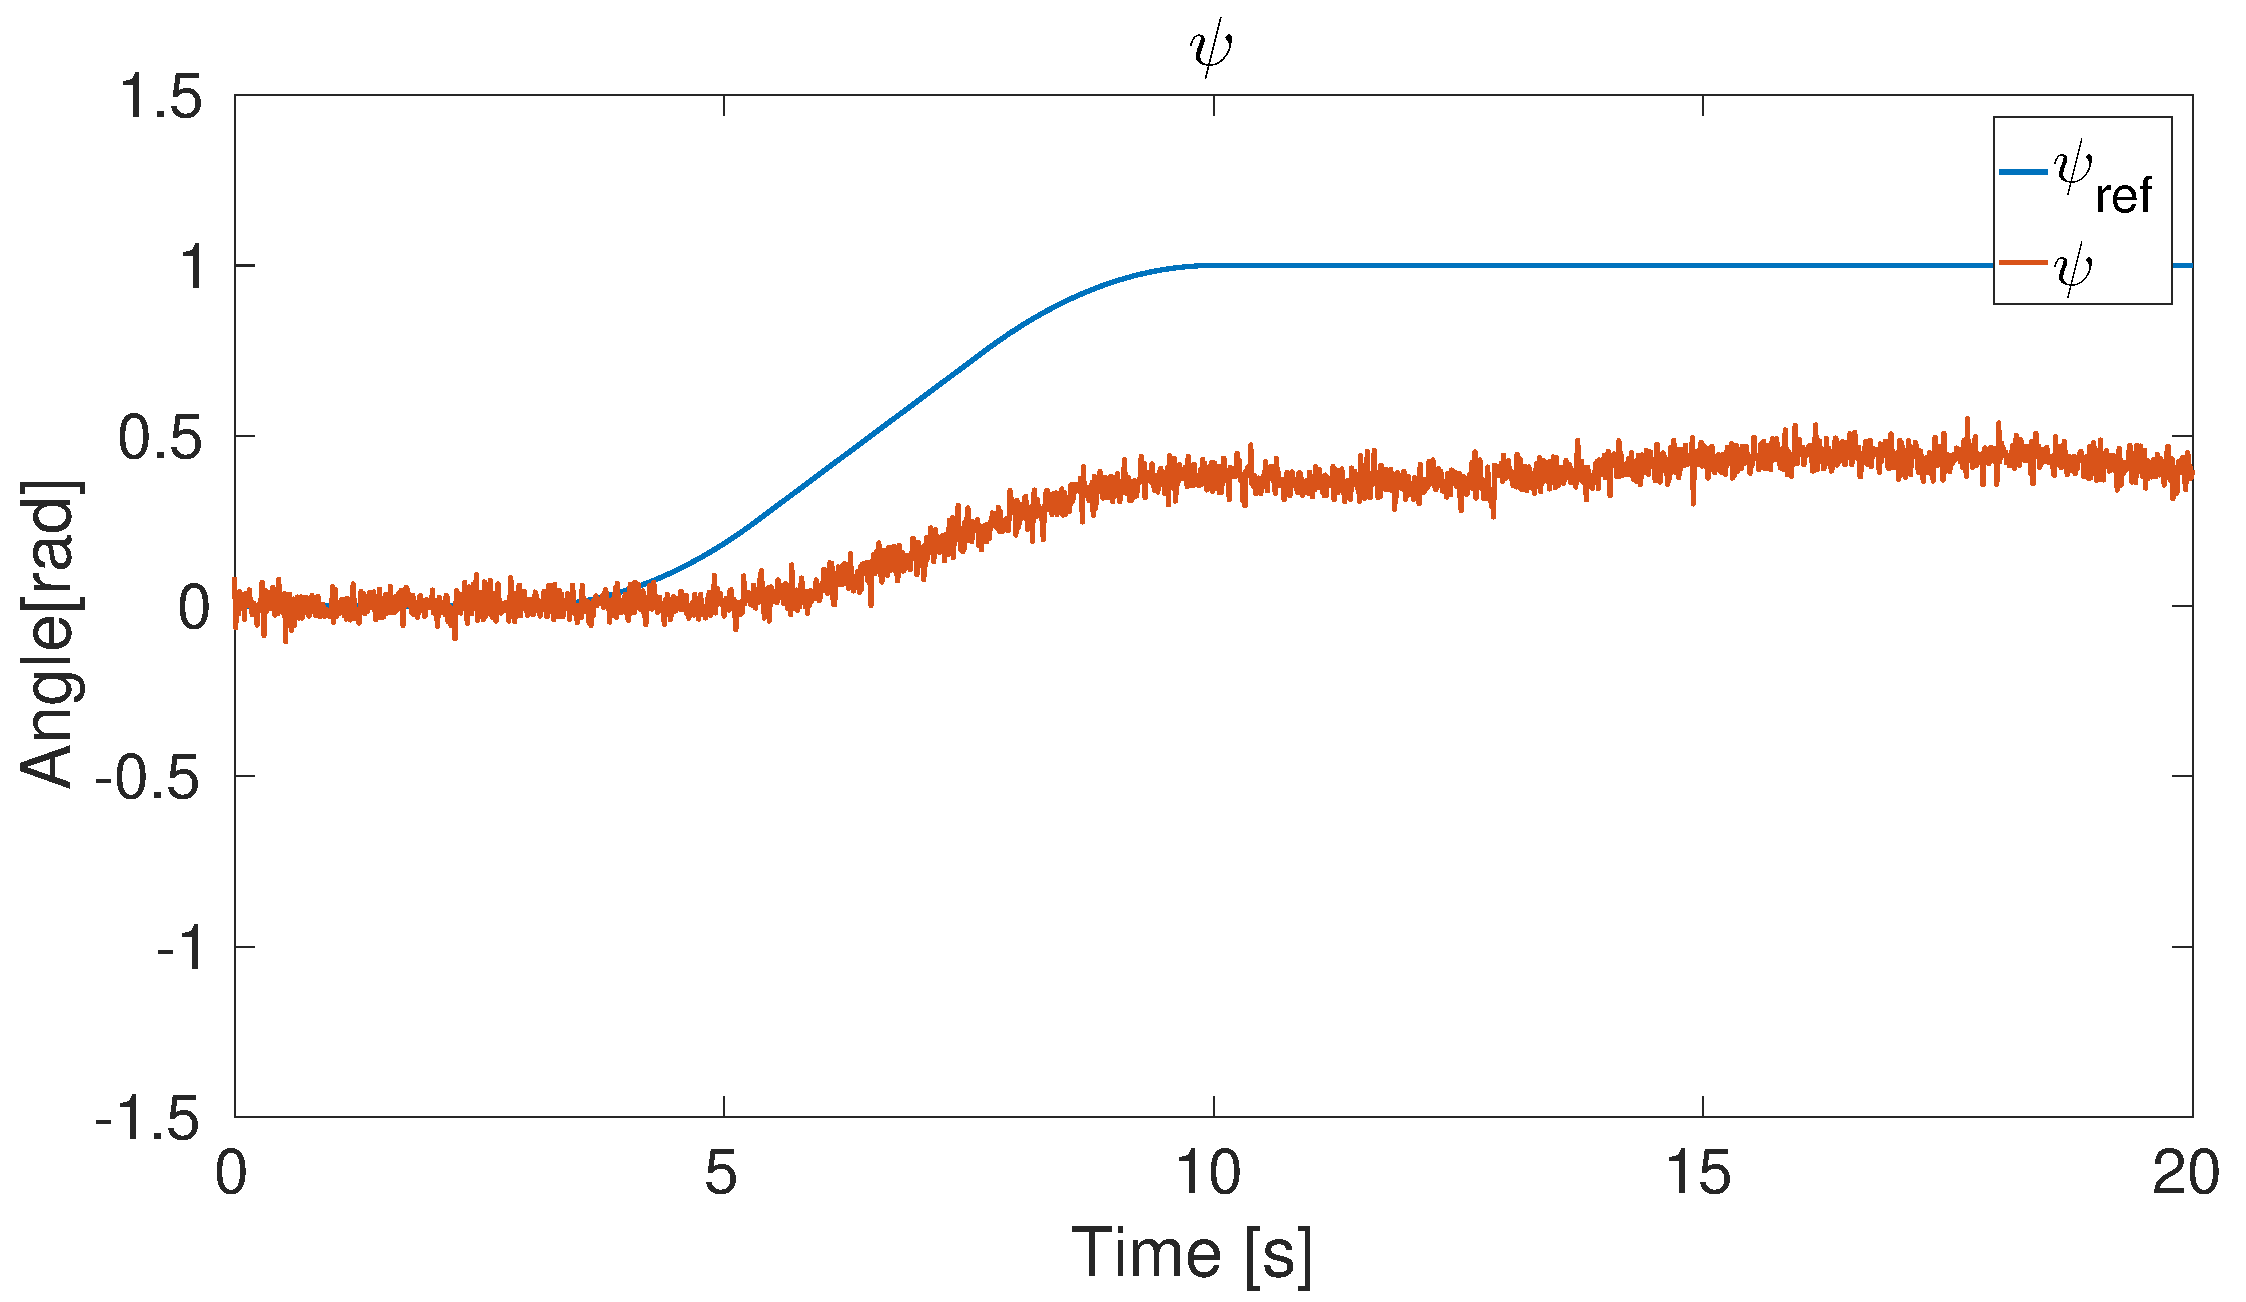
\includegraphics[width=0.4\textwidth]{simStepAllPsis3e10a1}}
  \caption{\label{fig:AppStepAllAttitude}% 
 A smooth steps with $q_{\text{0}} = 0$, $q_{\text{f}} = 1$, $t_{\text{s}} = 3$, $t_{\text{f}} = 15$ and $V = 1.5 (q_{\text{f}} - q_{\text{0}})/(t_{\text{f}} - t_{\text{s}}))$ was applied in all attitude angles at the same time while using the attitude controller.}
\end{figure}

\begin{figure}[tbp]
  \centering
  \subfloat[][\label{fig:ApptestSinRoll} Test response in $\rollAngle$.]{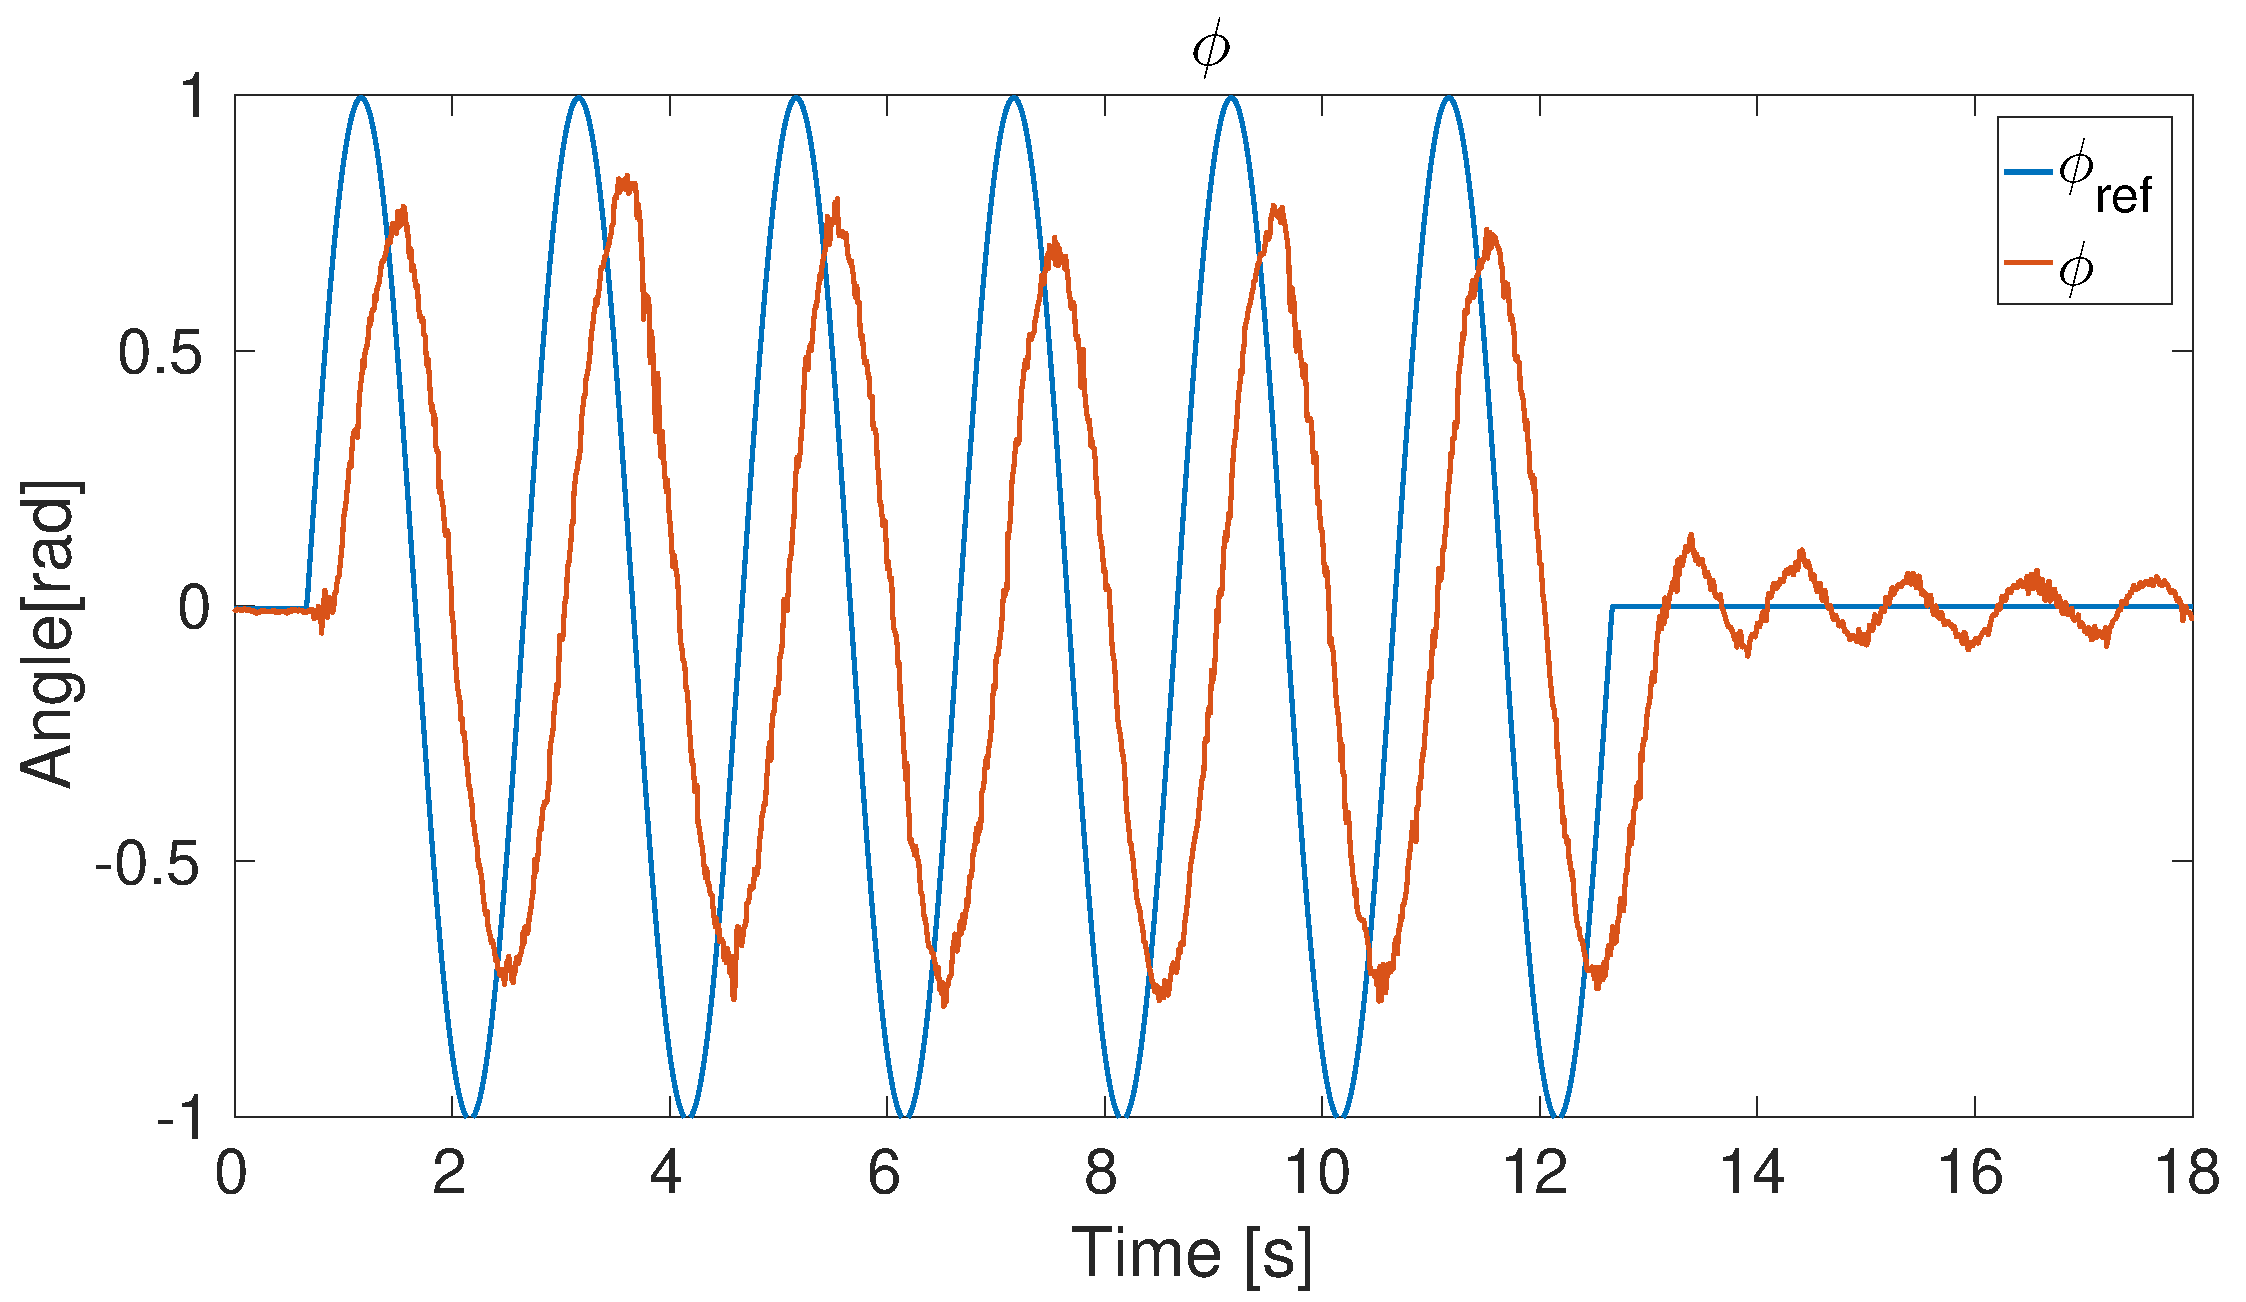
\includegraphics[width=0.4\textwidth]{testSinPhiA1}}
  \qquad
  \subfloat[][\label{fig:AppsimSinRoll} Simulated response in $\rollAngle$.]{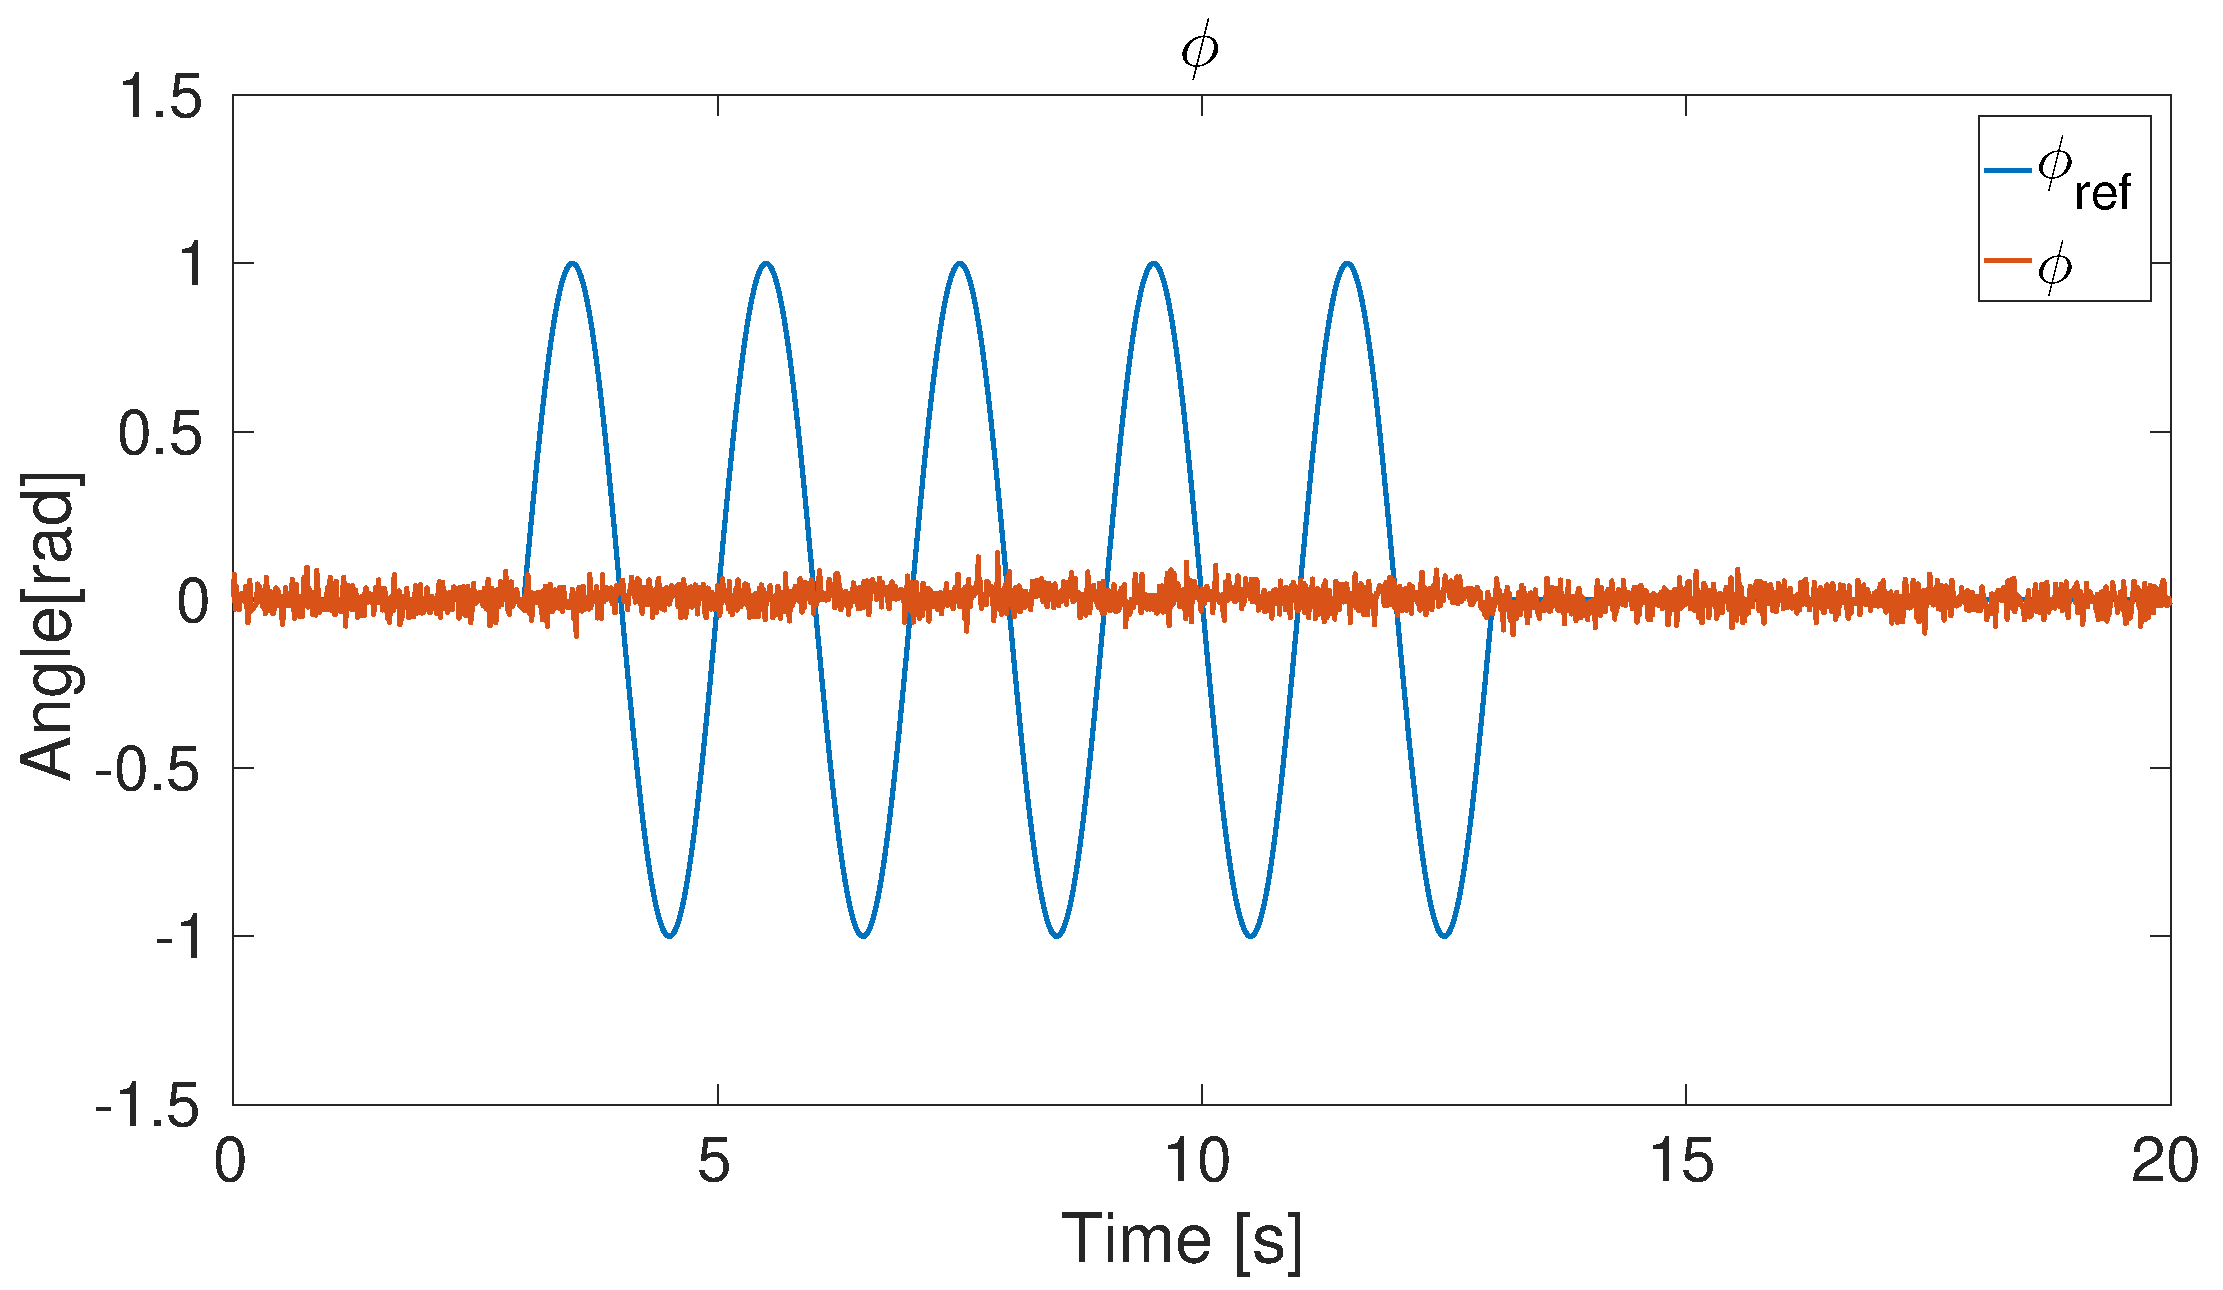
\includegraphics[width=0.4\textwidth]{simSinPhiA1}}
  \qquad
  \subfloat[][\label{fig:ApptestSinPitch} Test response in $\pitchAngle$.]{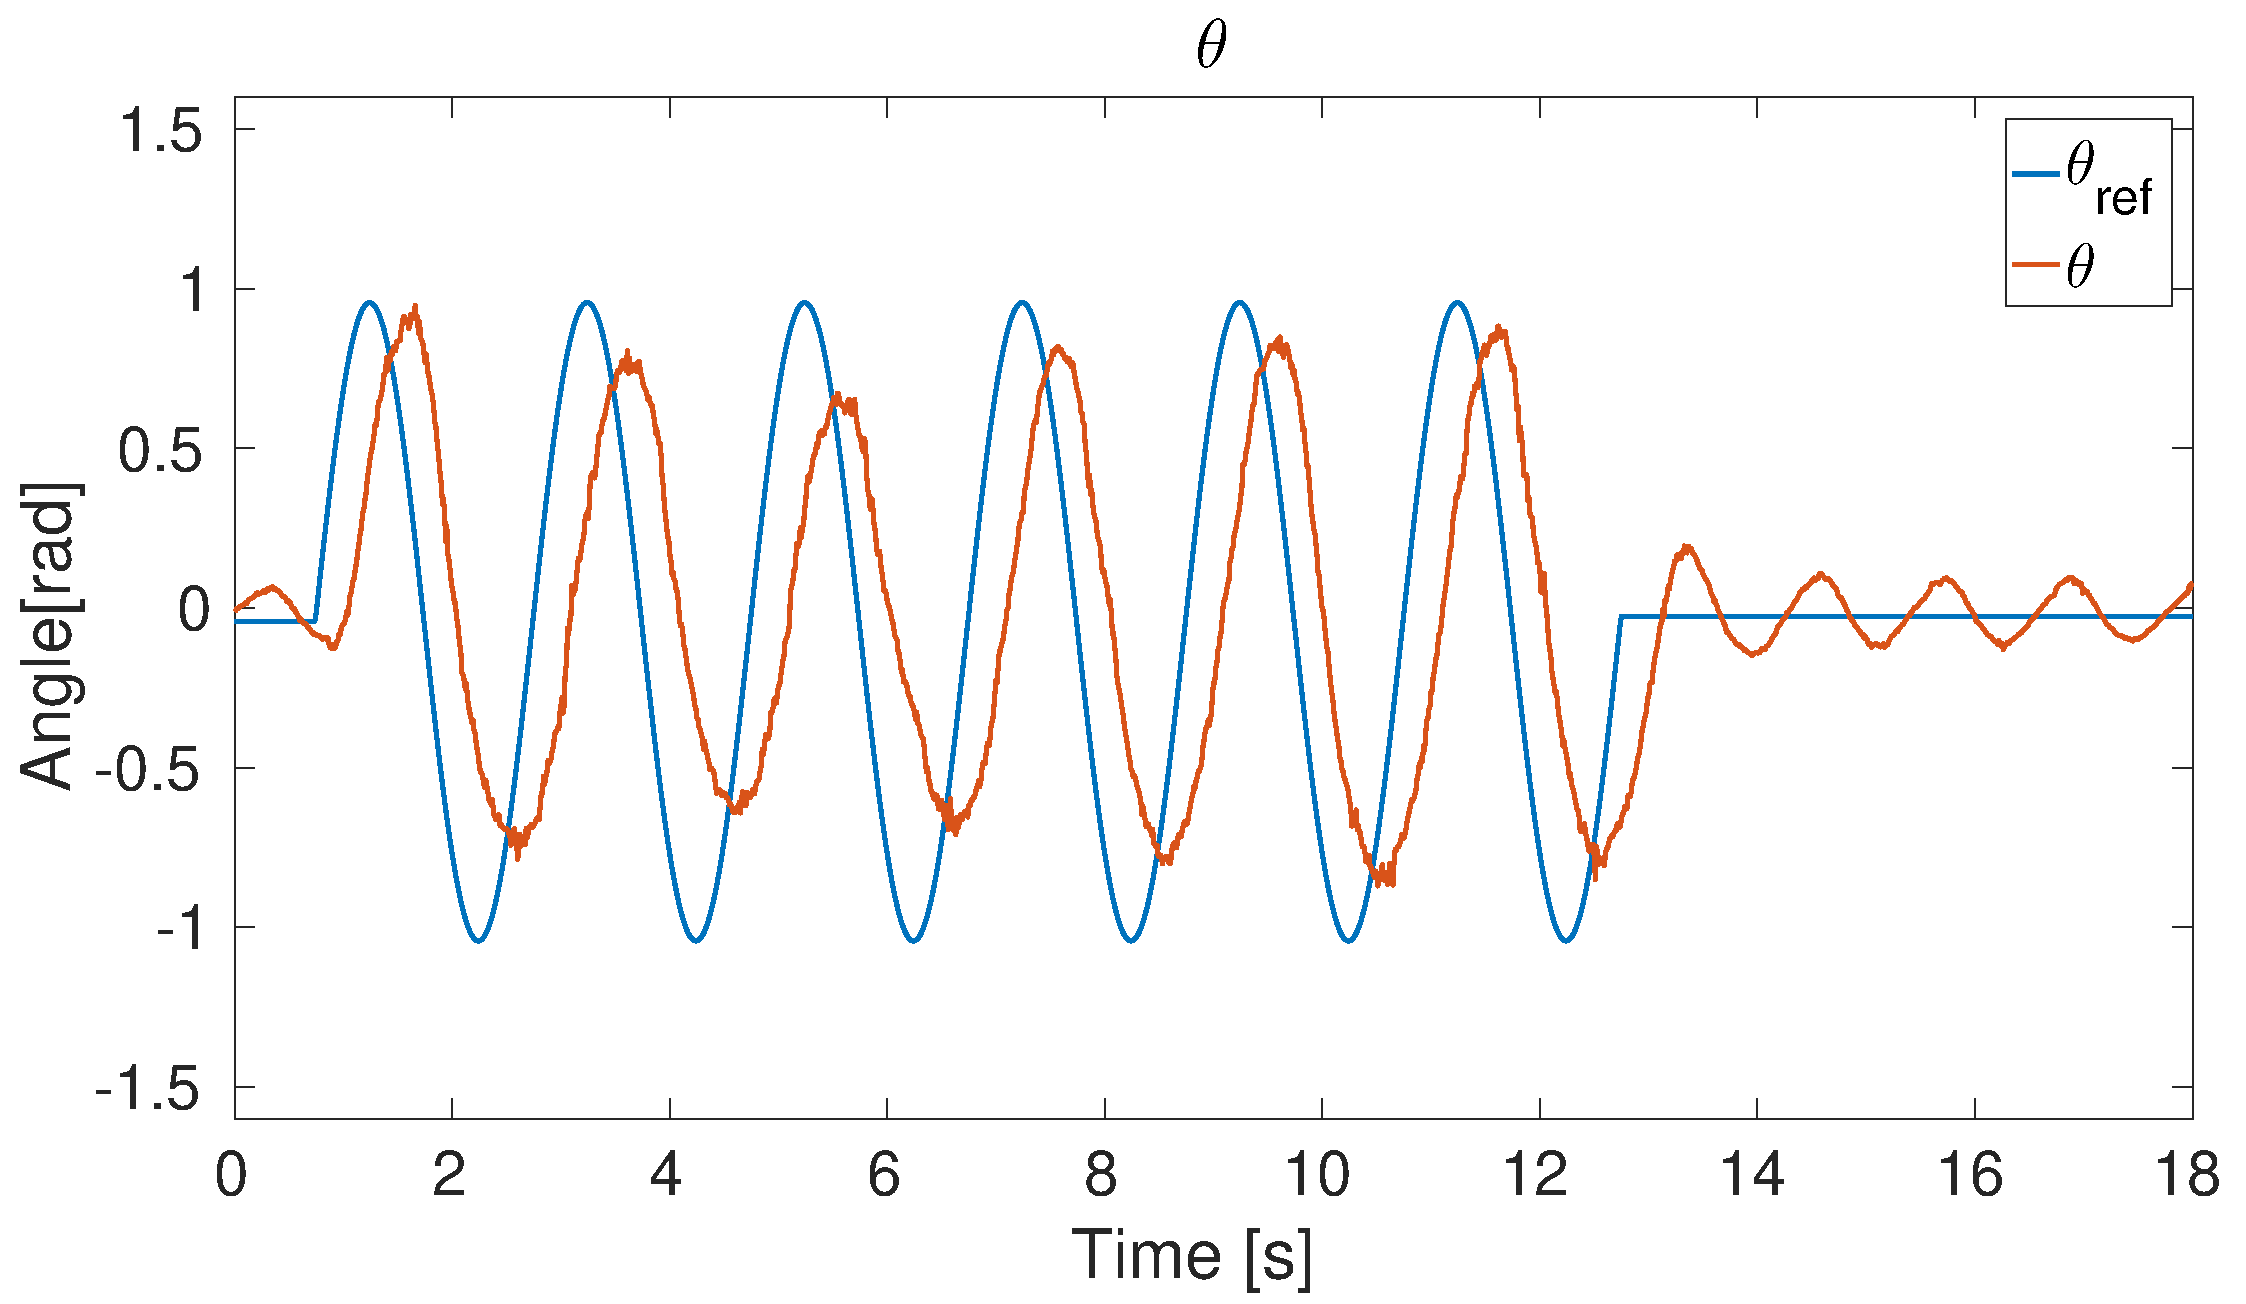
\includegraphics[width=0.4\textwidth]{testSinThetaA1}}
  \qquad
  \subfloat[][\label{fig:AppsimSinPitch} Simulated response in $\pitchAngle$.]{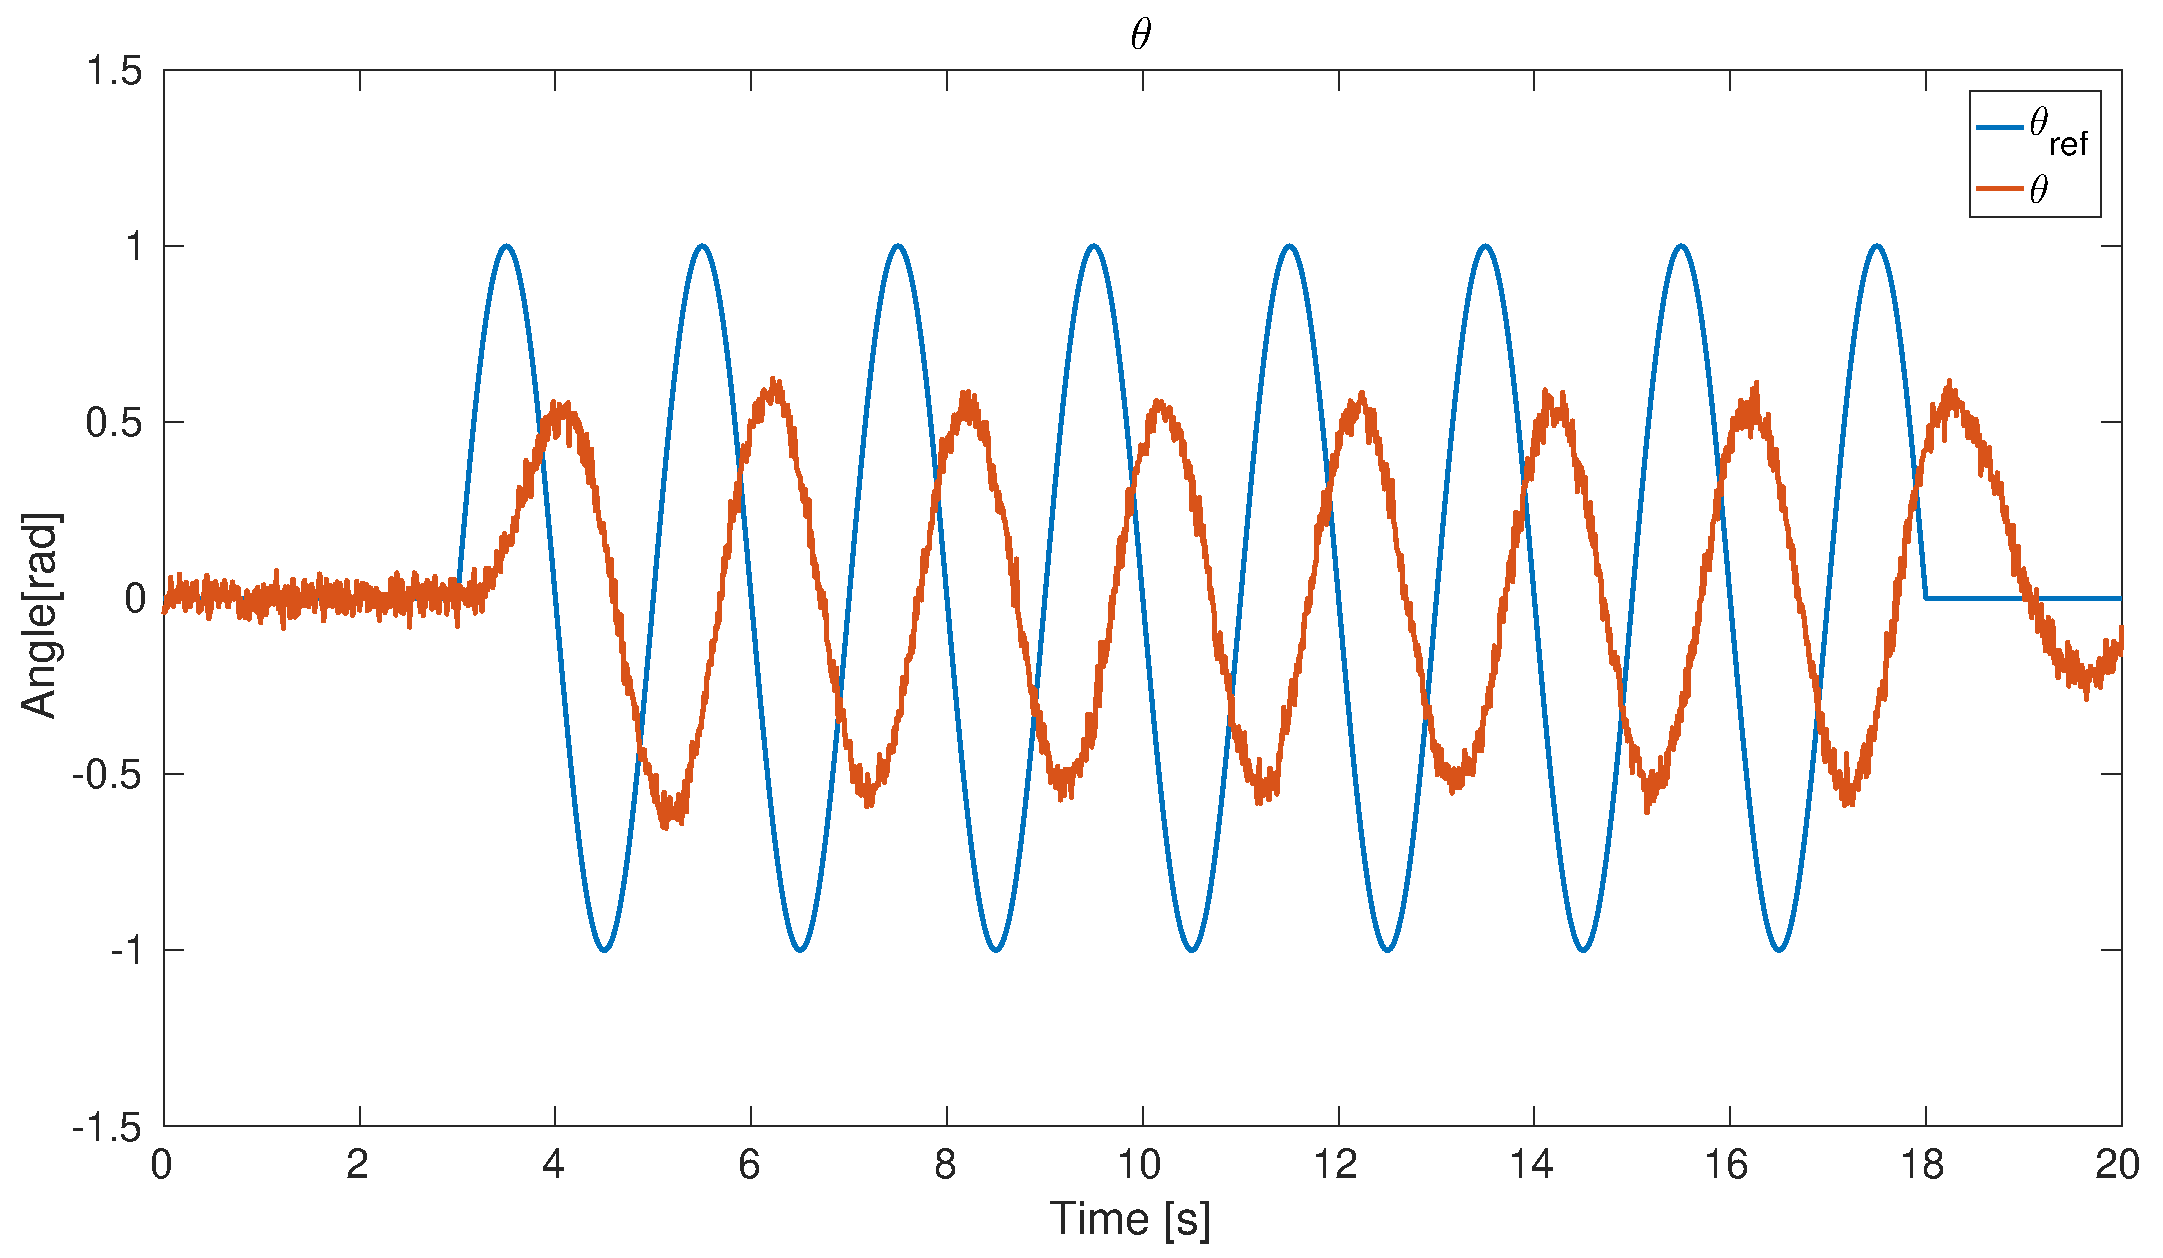
\includegraphics[width=0.4\textwidth]{simSinThetaA1}}
  \qquad
  \subfloat[][\label{fig:ApptestSinYaw} Test response in $\yawAngle$.]{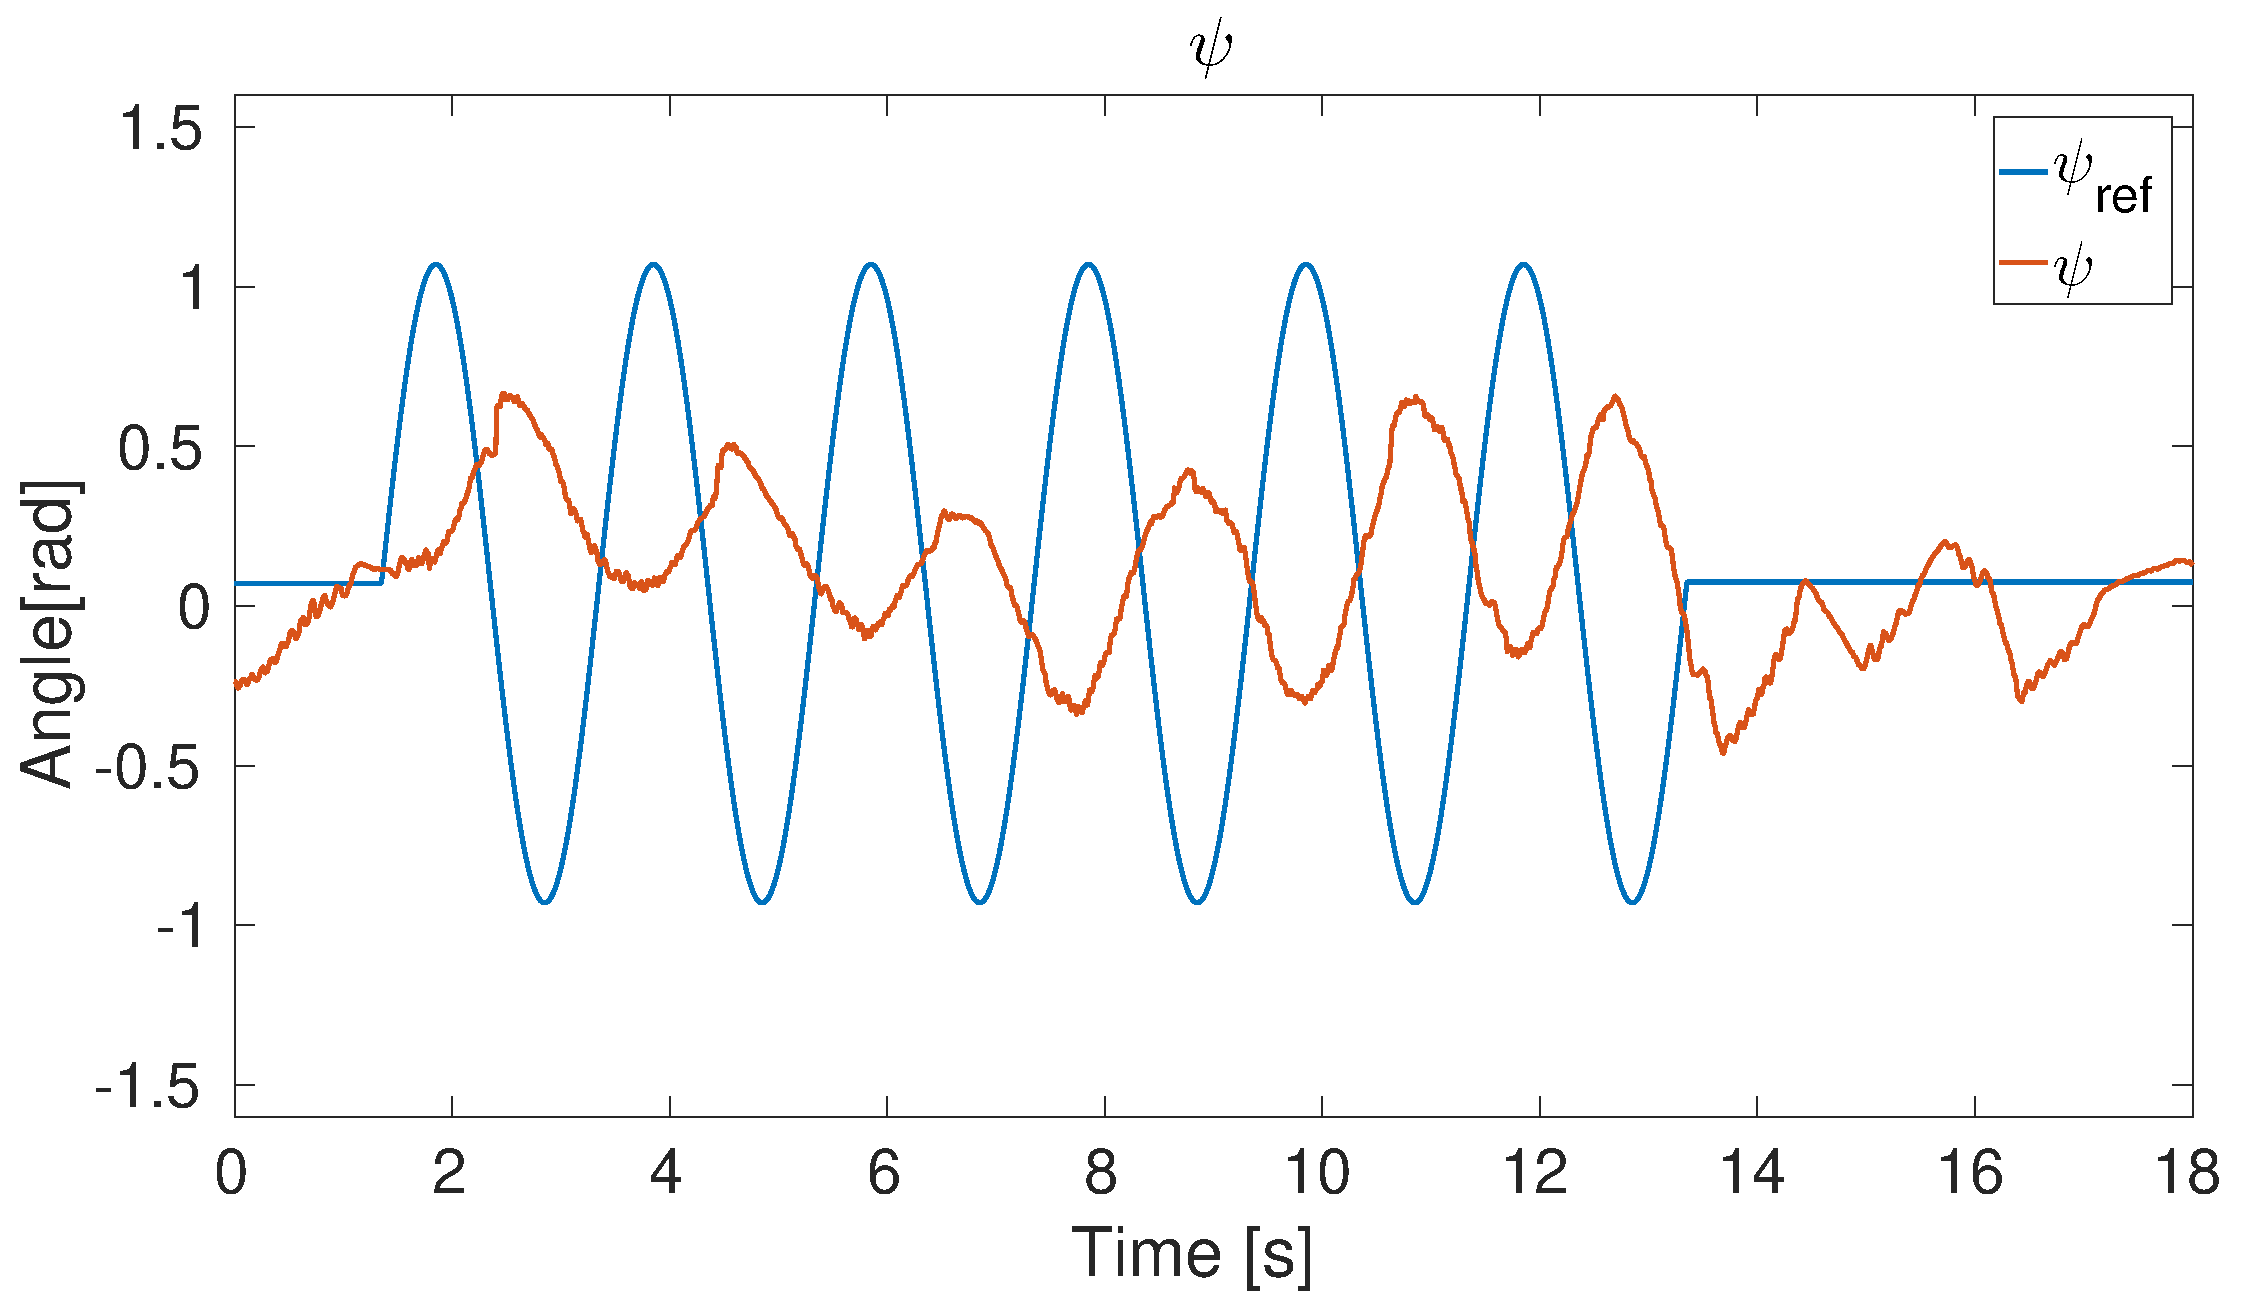
\includegraphics[width=0.4\textwidth]{testSinPsiA1}}
  \qquad
  \subfloat[][\label{fig:AppsimSinYaw} Simulated response in $\yawAngle$.]{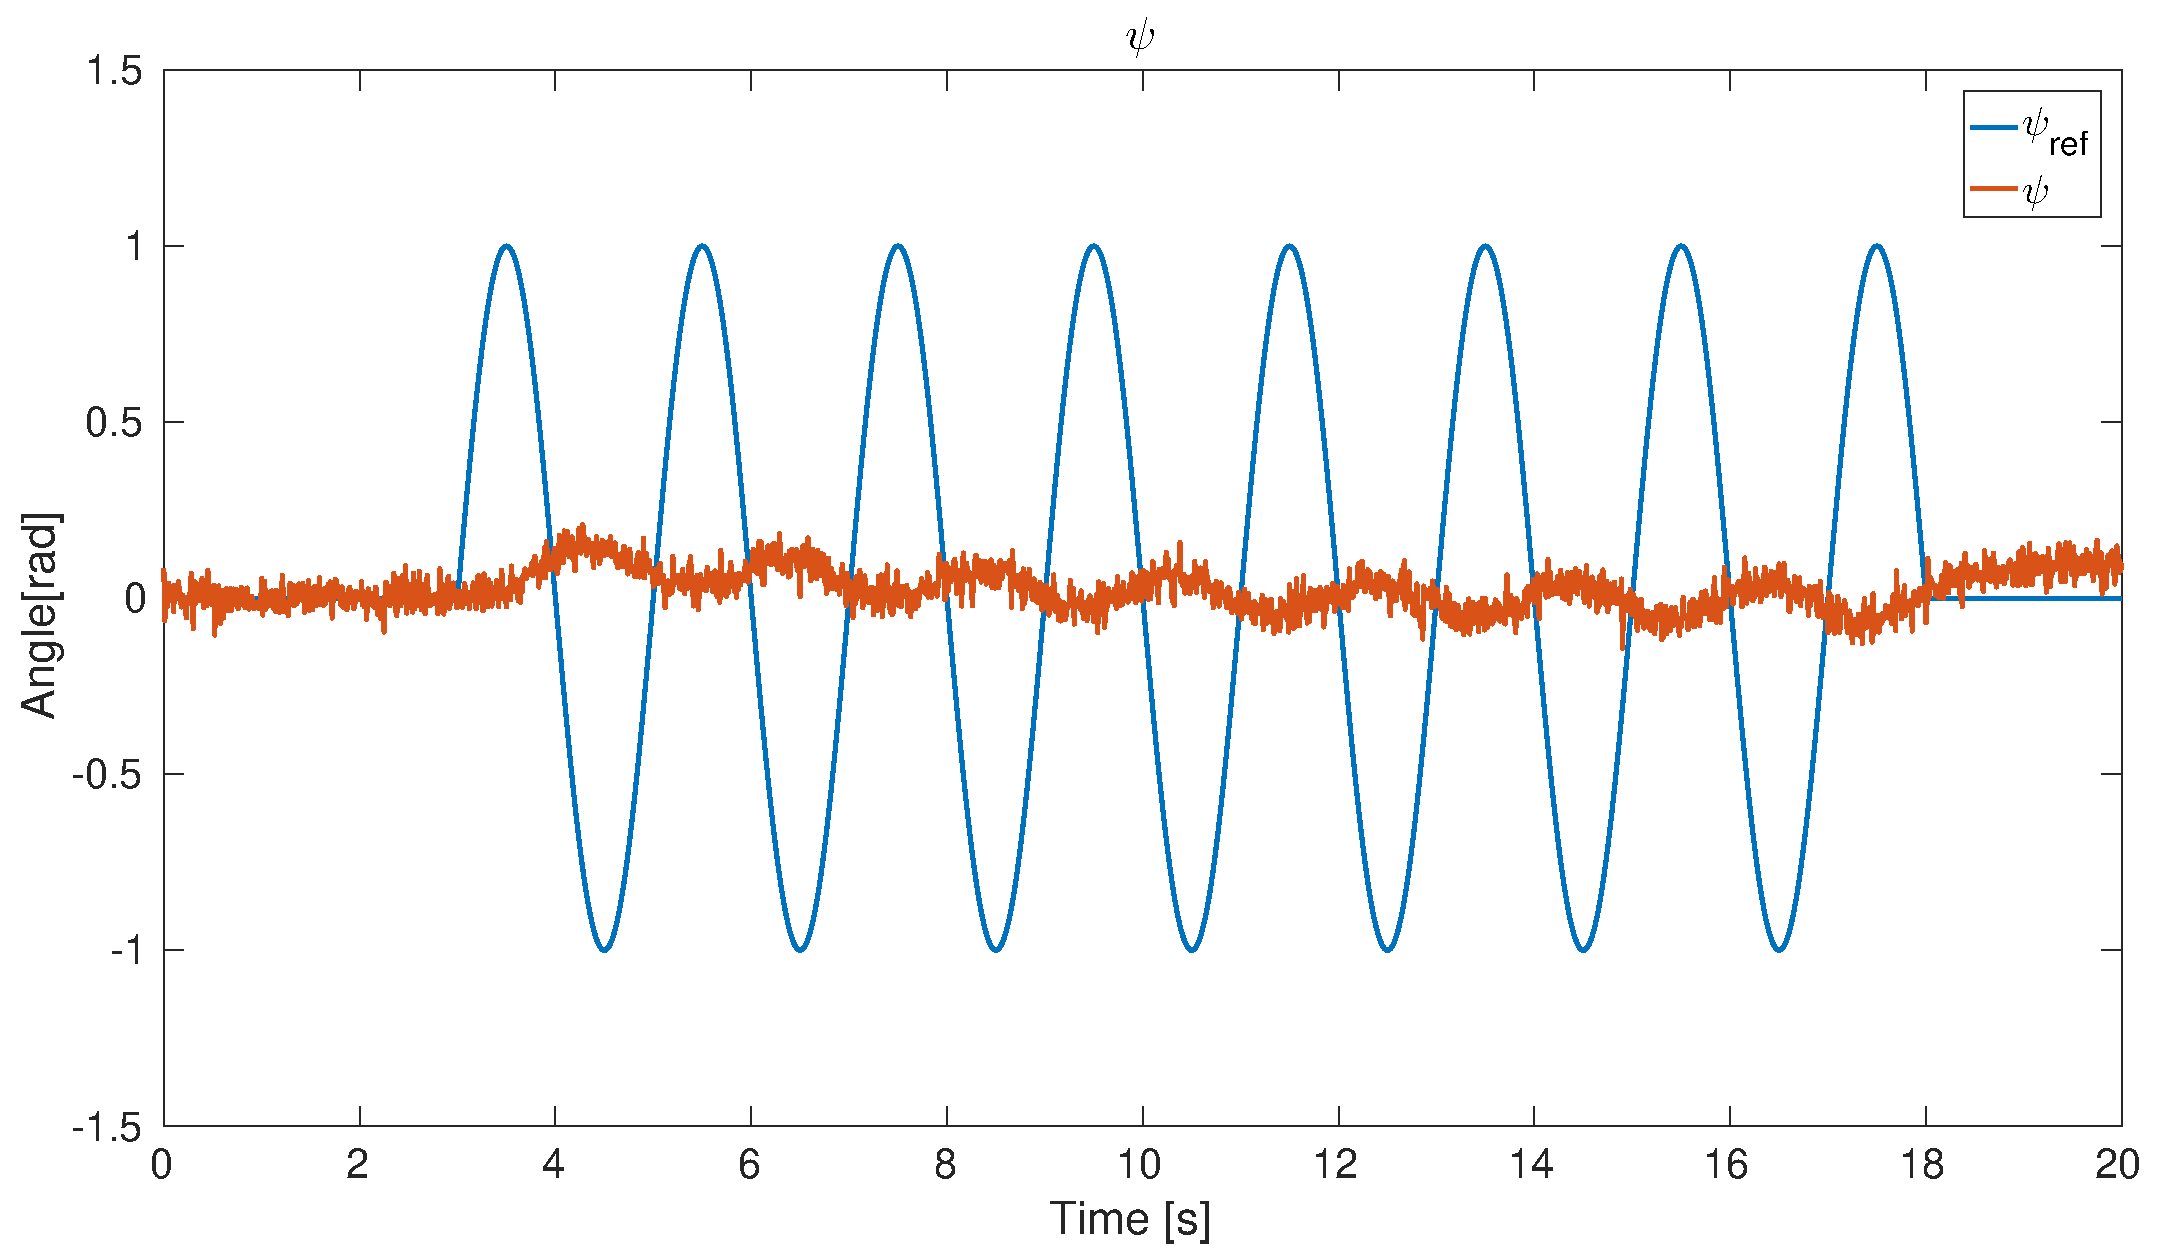
\includegraphics[width=0.4\textwidth]{simSinPsiA1}}
    \caption{\label{fig:AppSin1Attitude}% 
   A sine signal with amplitude $1$ and frequency $0.5\ \hertz$ was applied in one attitude angle at a time while using the attitude controller. While a sine signal was applied in one attitude angle the other attitude angles were not controlled.}
\end{figure}

\begin{figure}
\centering
  \subfloat[][\label{fig:ApptestSinAllRollAttitude} Test response in $\rollAngle$.]{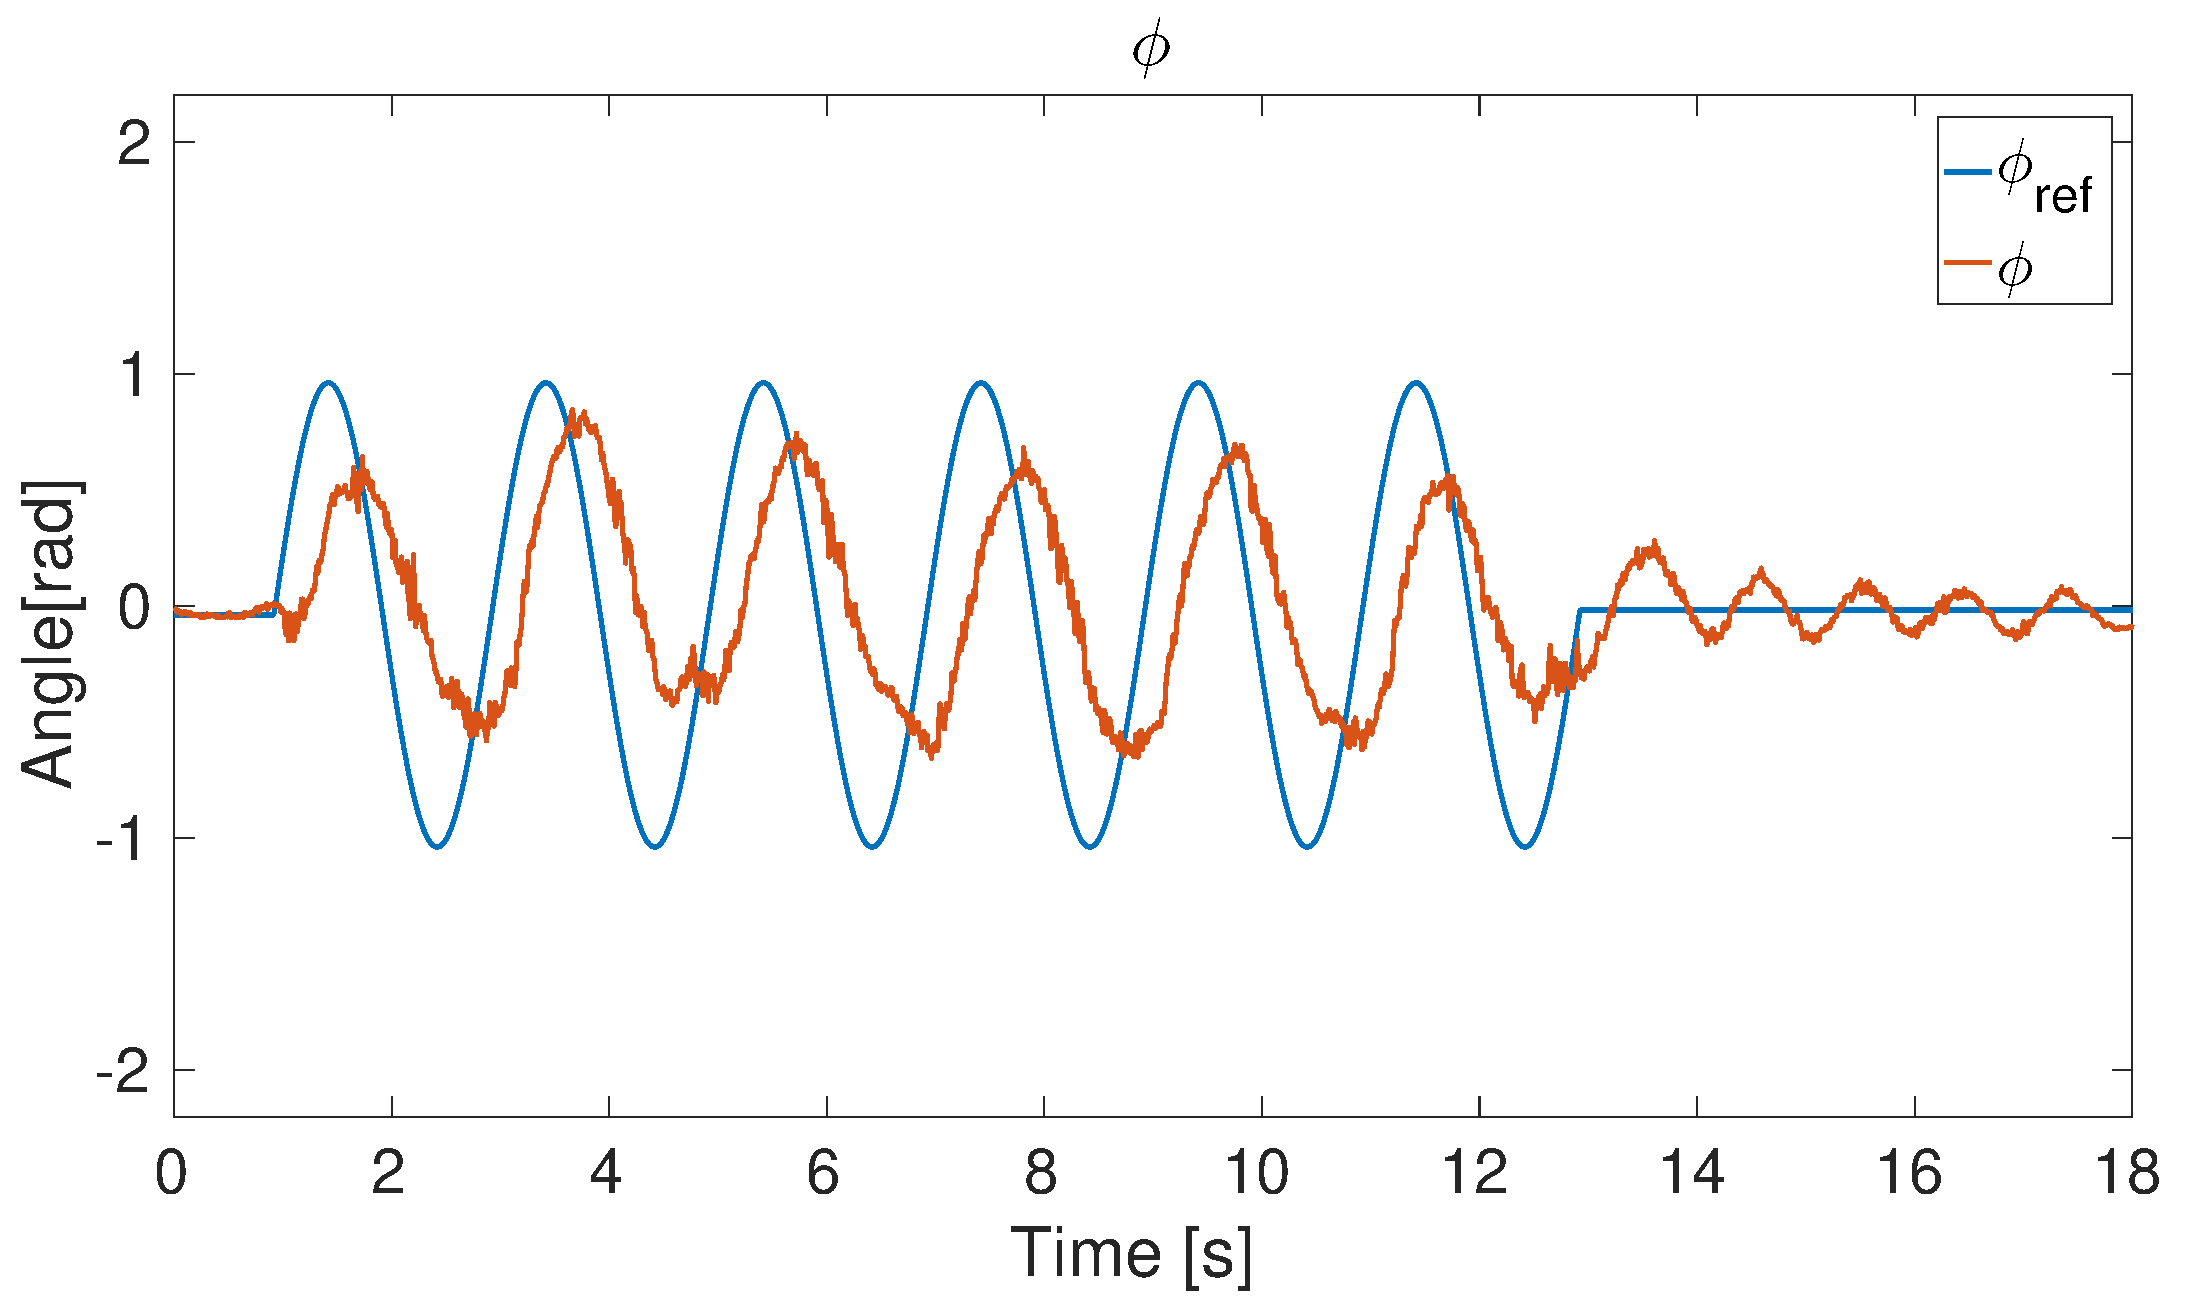
\includegraphics[width=0.4\textwidth]{testSinAllPhiA1}}
  \qquad
  \subfloat[][\label{fig:AppsimSinAllRollAttitude} Simulated response in $\rollAngle$.]{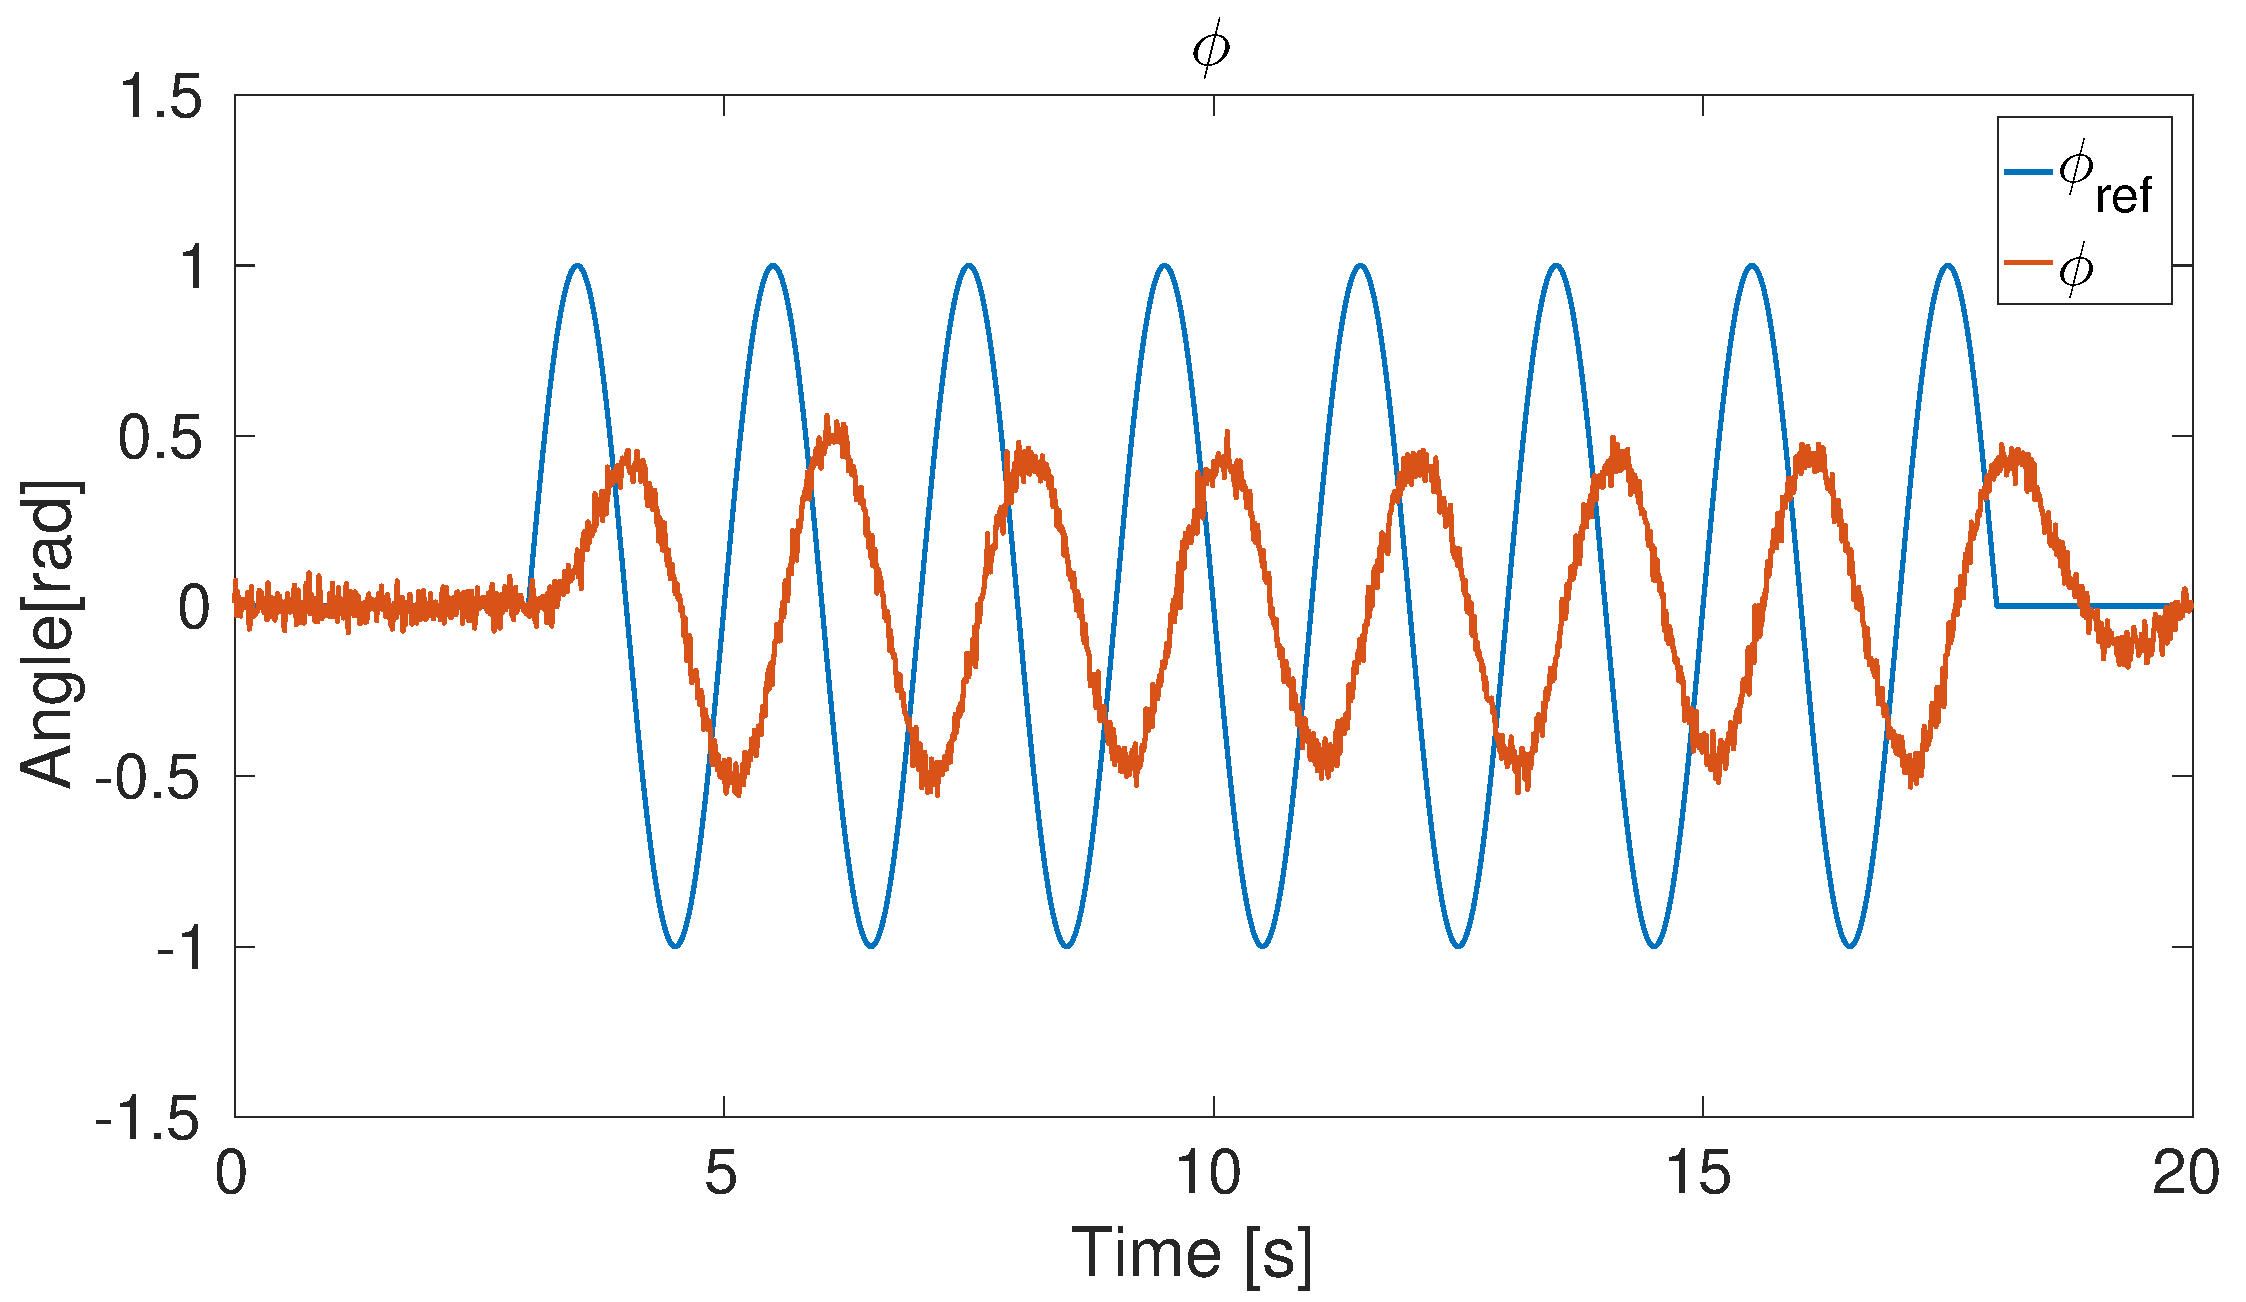
\includegraphics[width=0.4\textwidth]{simSinAllPhiA1}}
  \qquad
  \subfloat[][\label{fig:ApptestSinAllPitchAttitude} Test response in $\pitchAngle$.]{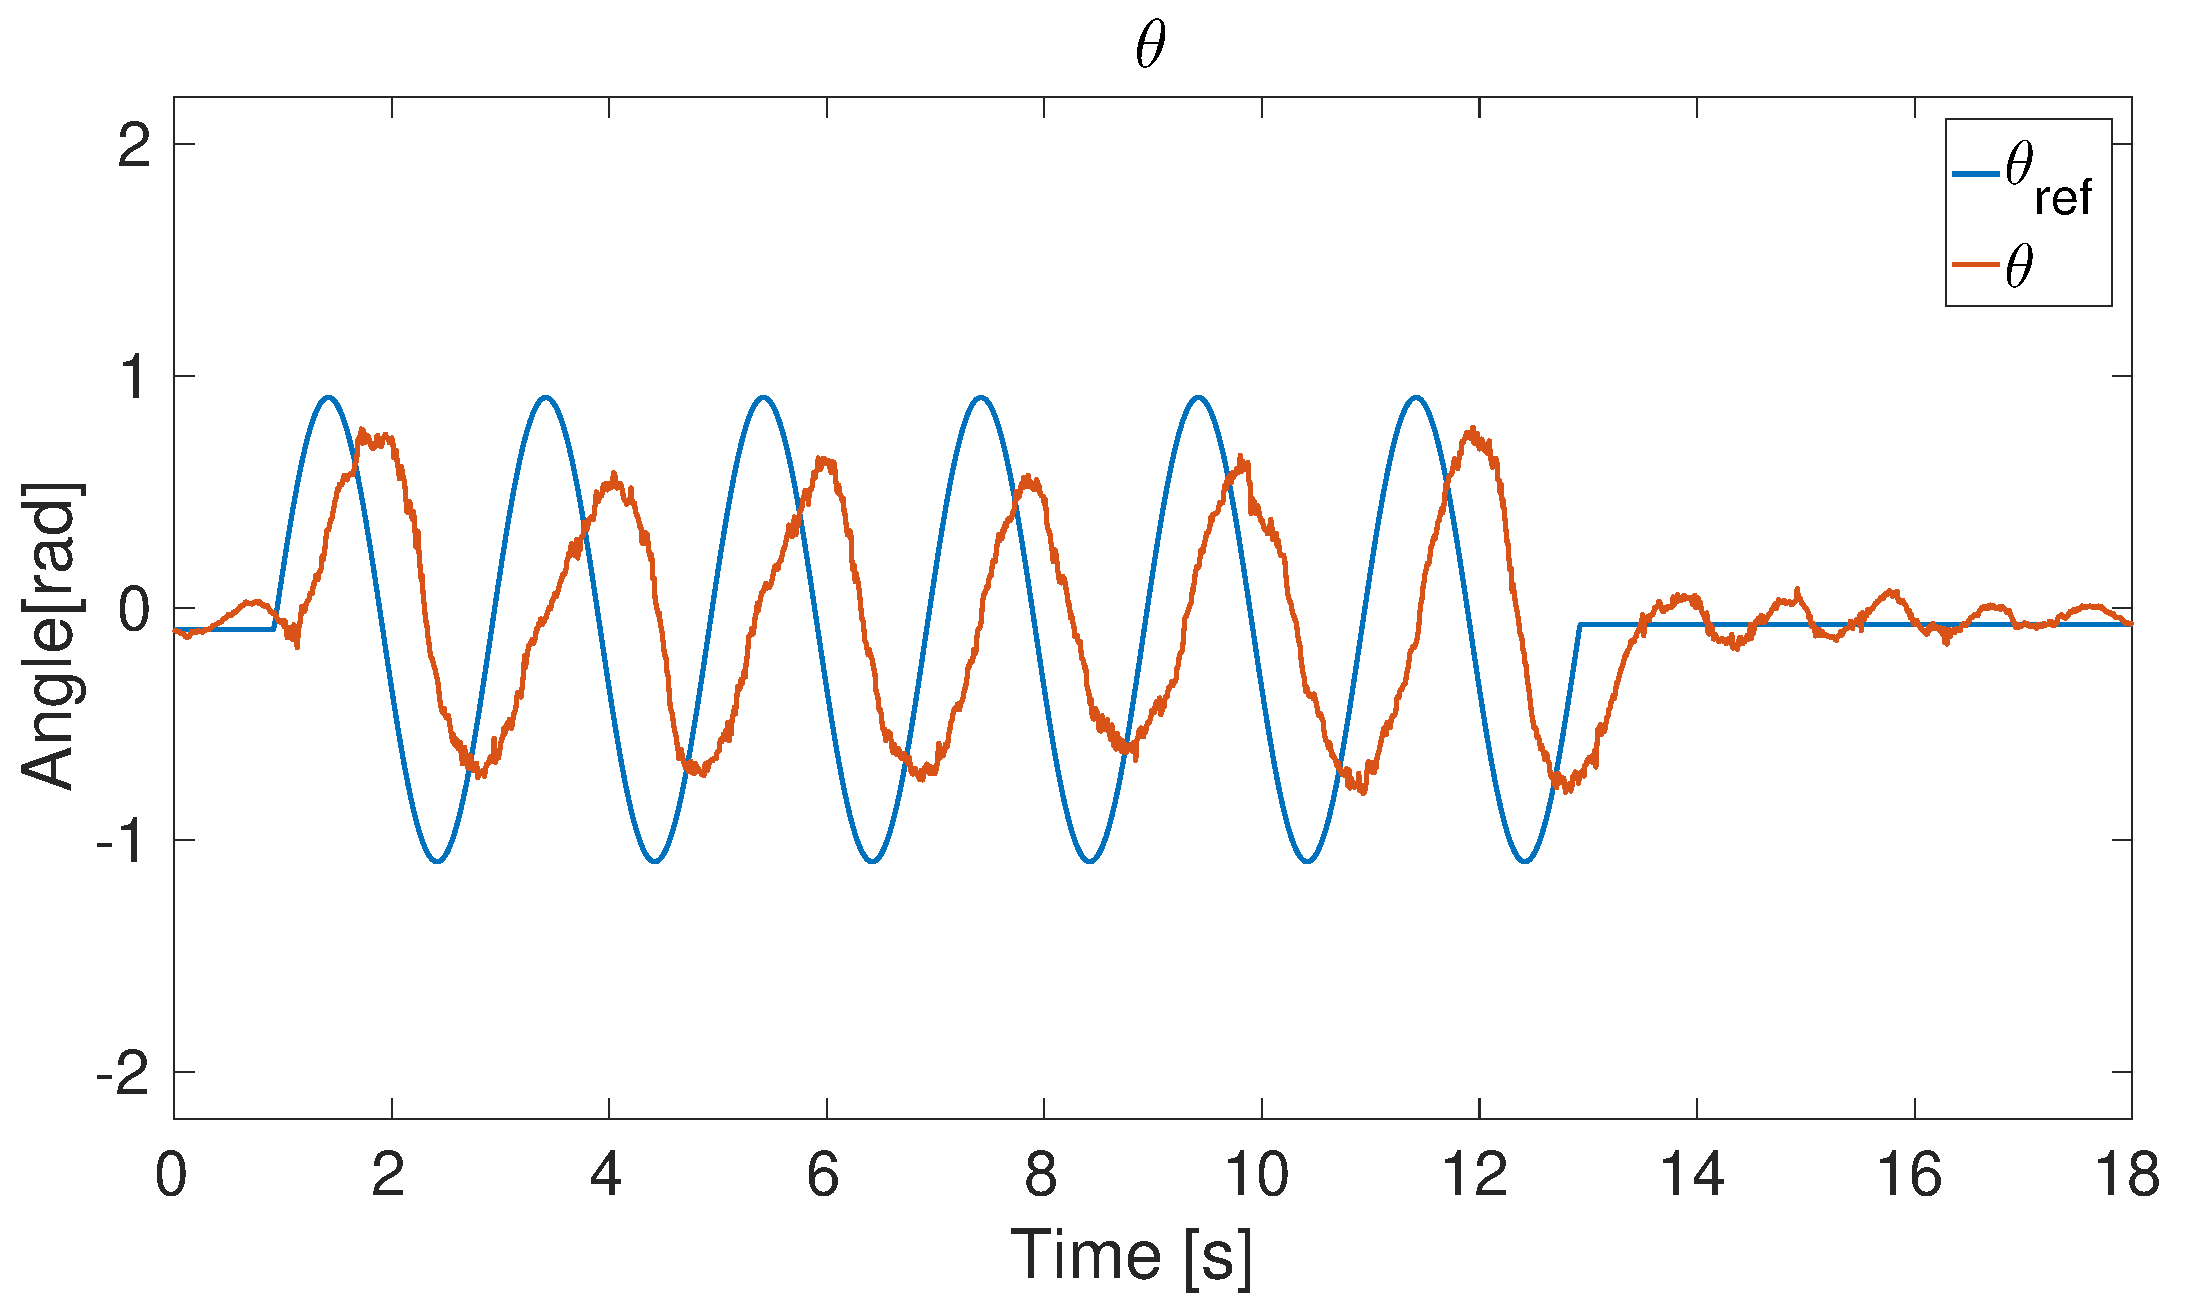
\includegraphics[width=0.4\textwidth]{testSinAllThetaA1}}
  \qquad
  \subfloat[][\label{fig:AppsimSinAllPitchAttitude} Simulated response in $\pitchAngle$.]{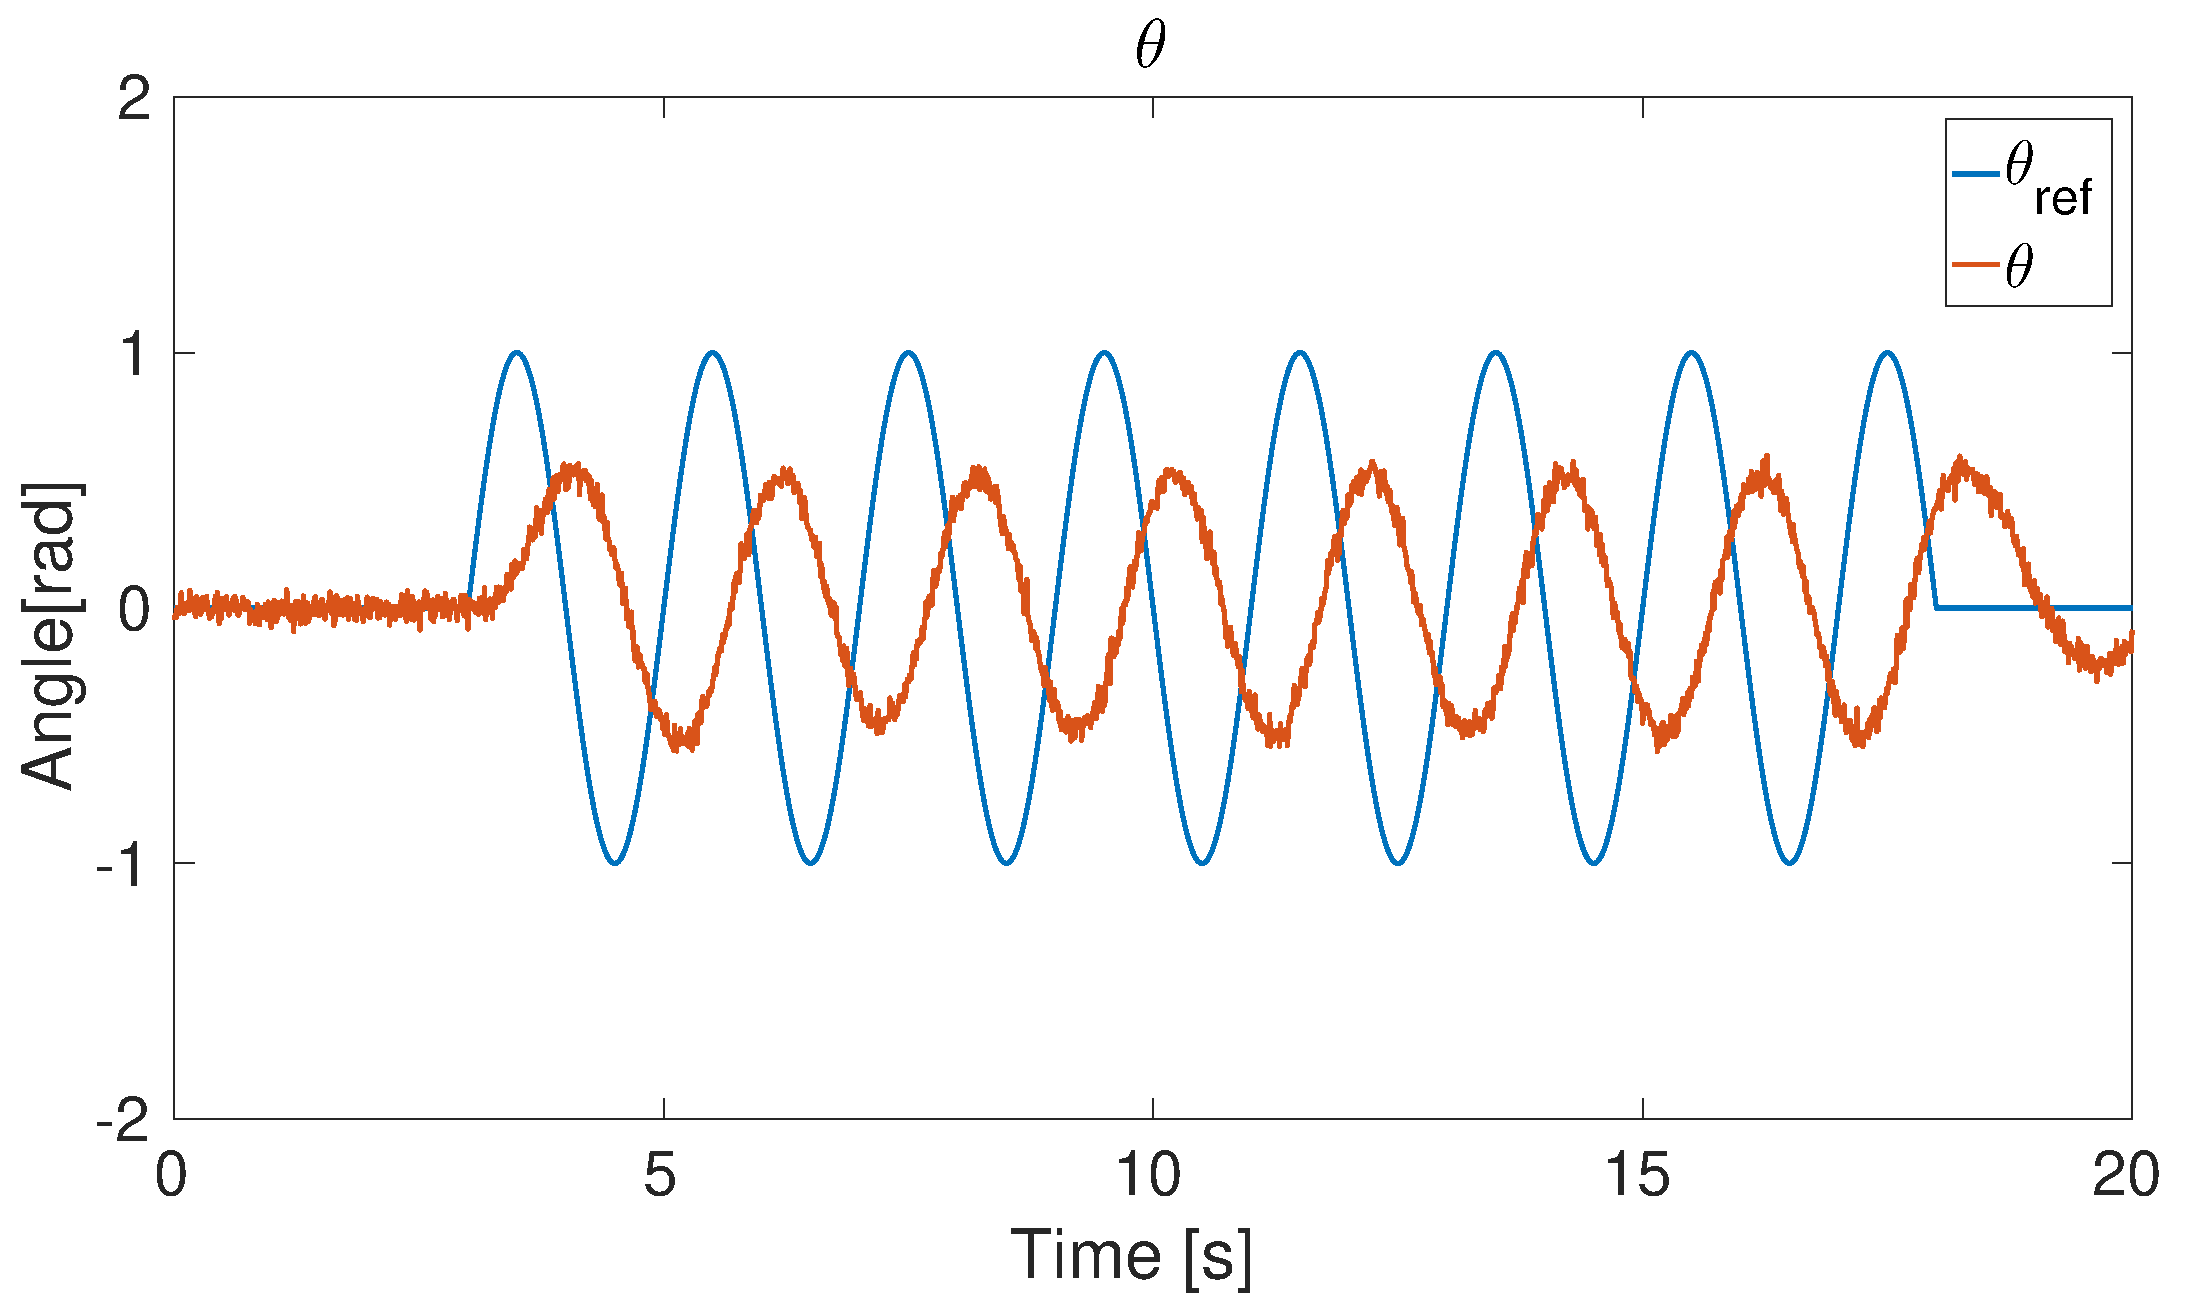
\includegraphics[width=0.4\textwidth]{simSinAllThetaA1}}
  \qquad
  \subfloat[][\label{fig:ApptestSinAllYawAttitude} Test response in $\yawAngle$.]{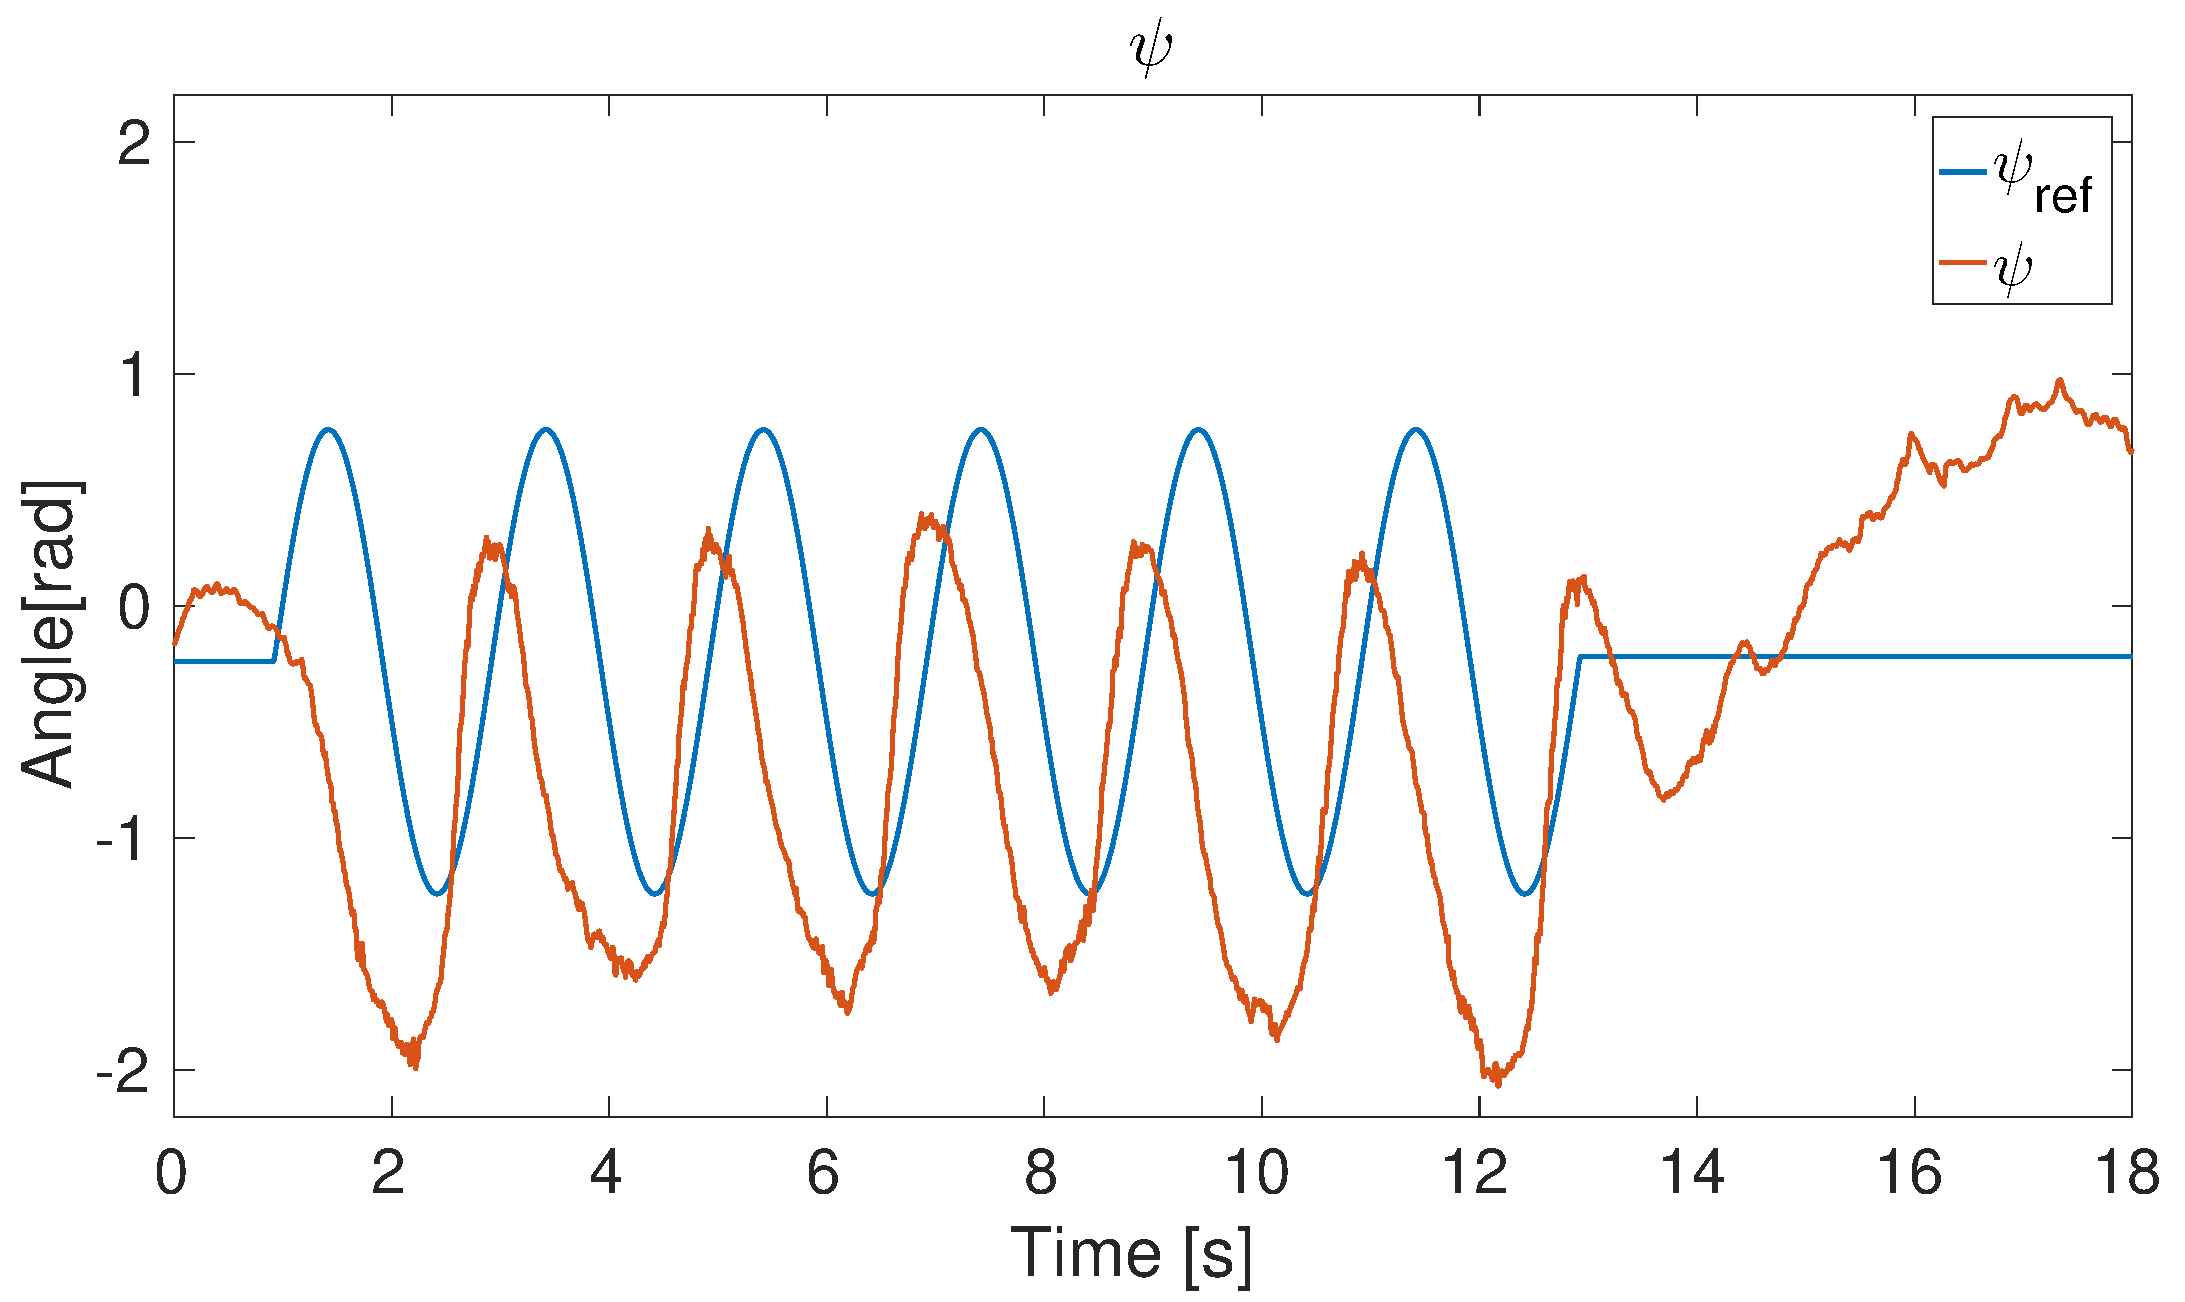
\includegraphics[width=0.4\textwidth]{testSinAllPsiA1}}
  \qquad
  \subfloat[][\label{fig:AppsimSinAllYawAttitude} Simulated response in $\yawAngle$.]{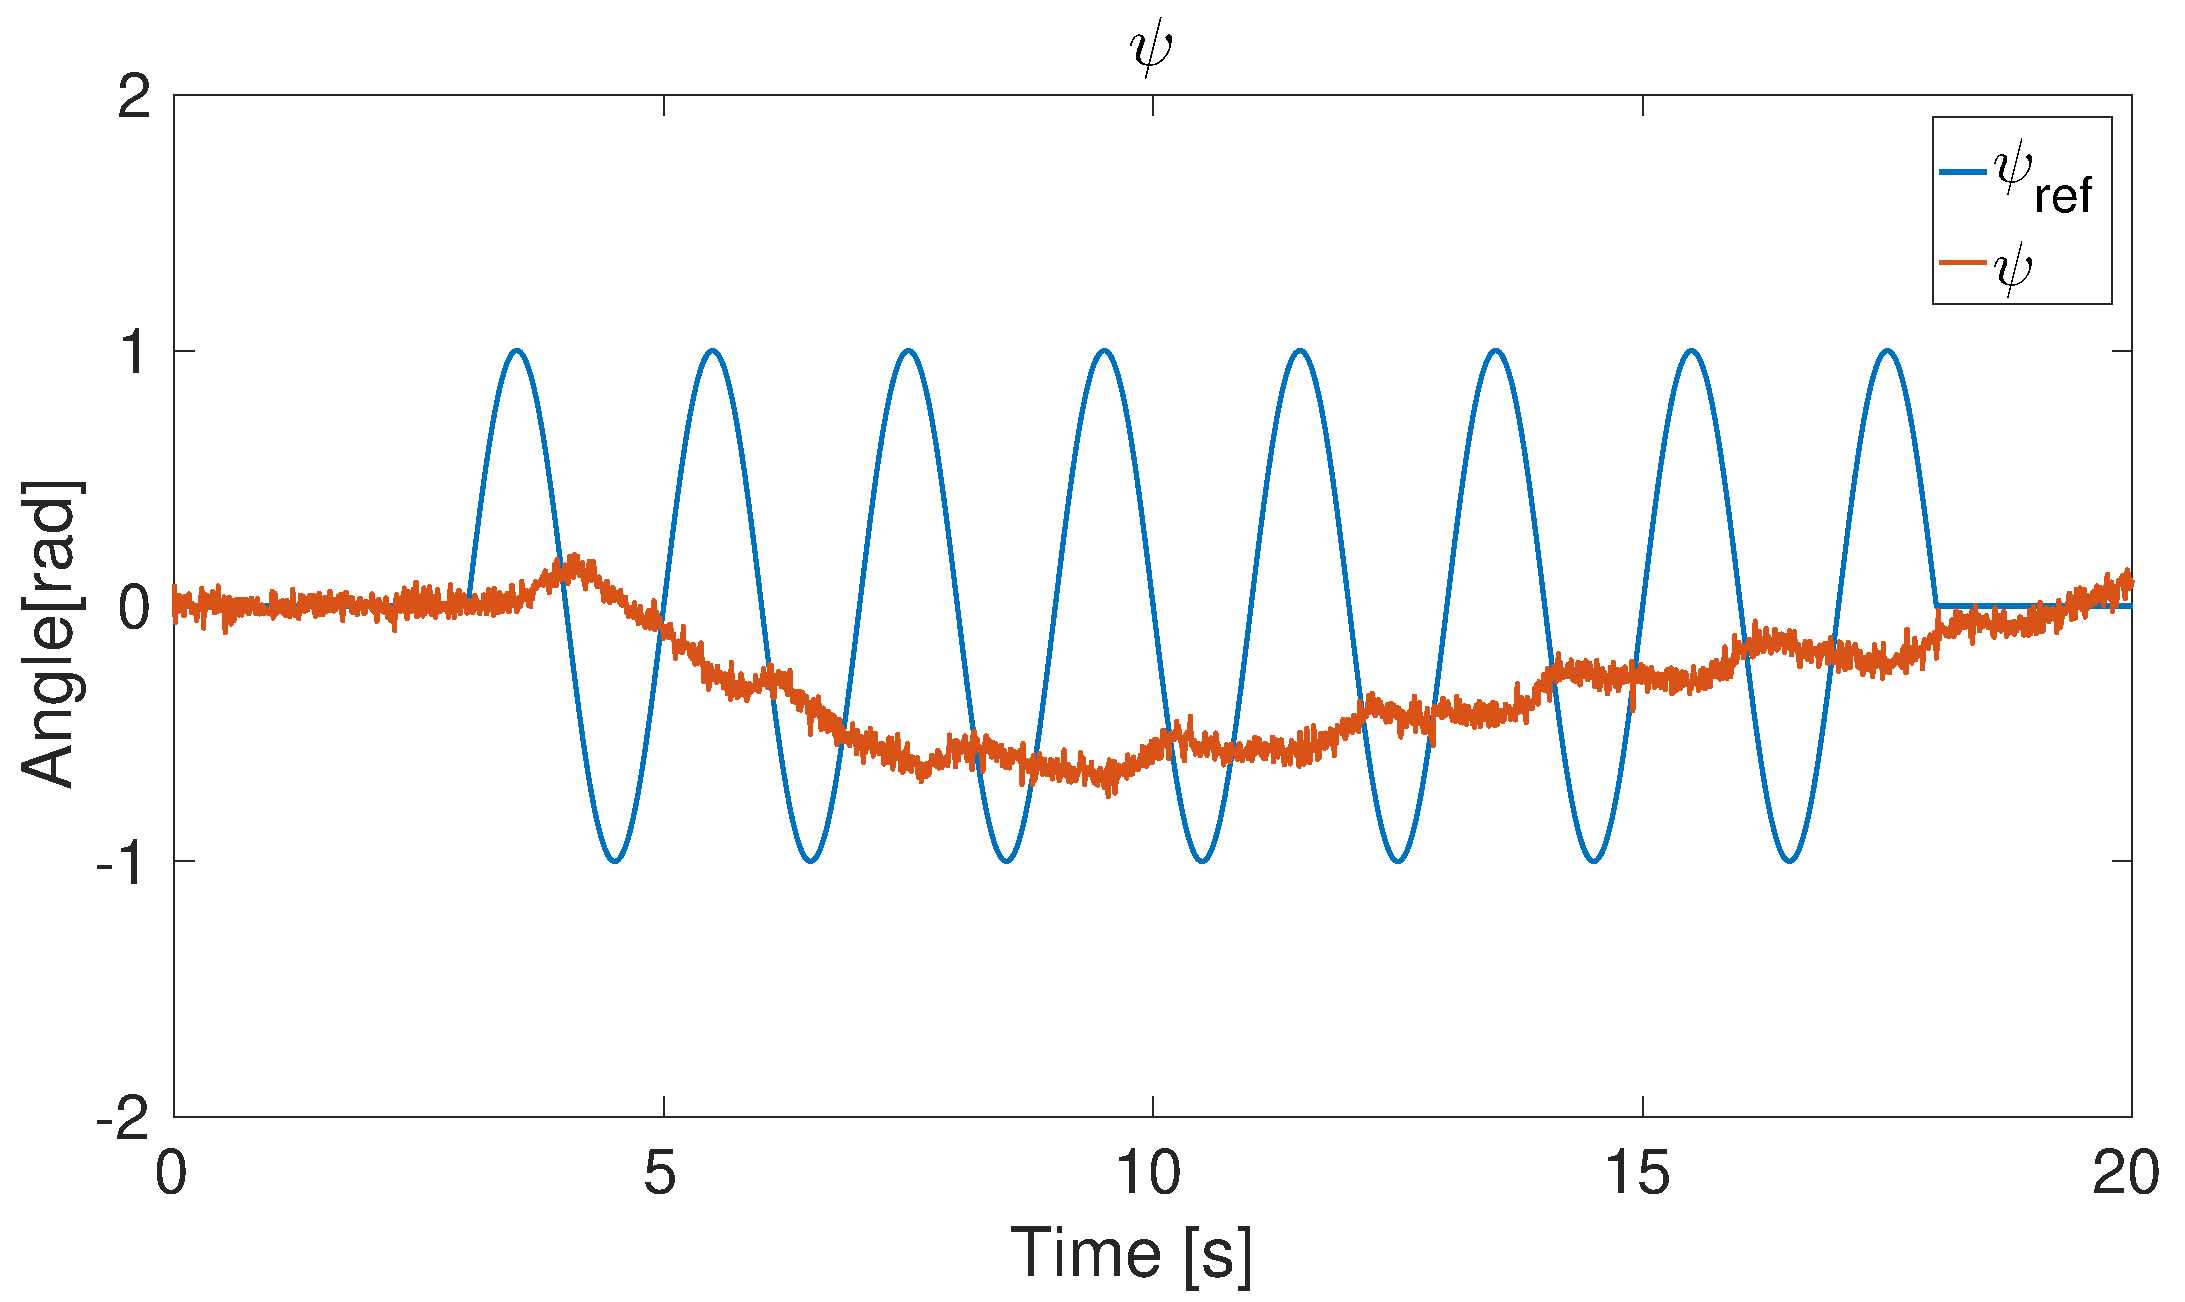
\includegraphics[width=0.4\textwidth]{simSinAllPsiA1}}
  \caption{\label{fig:AppSinAllAttitude}%
   A sine signal with amplitude $1$ and frequency $0.5\ \hertz$ was applied in all attitude angles at the same time while using the attitude controller.}
\end{figure}


\begin{figure}[tbp]
  \centering
  \subfloat[][\label{fig:ApptestSin05Roll} Test response in $\rollAngle$.]{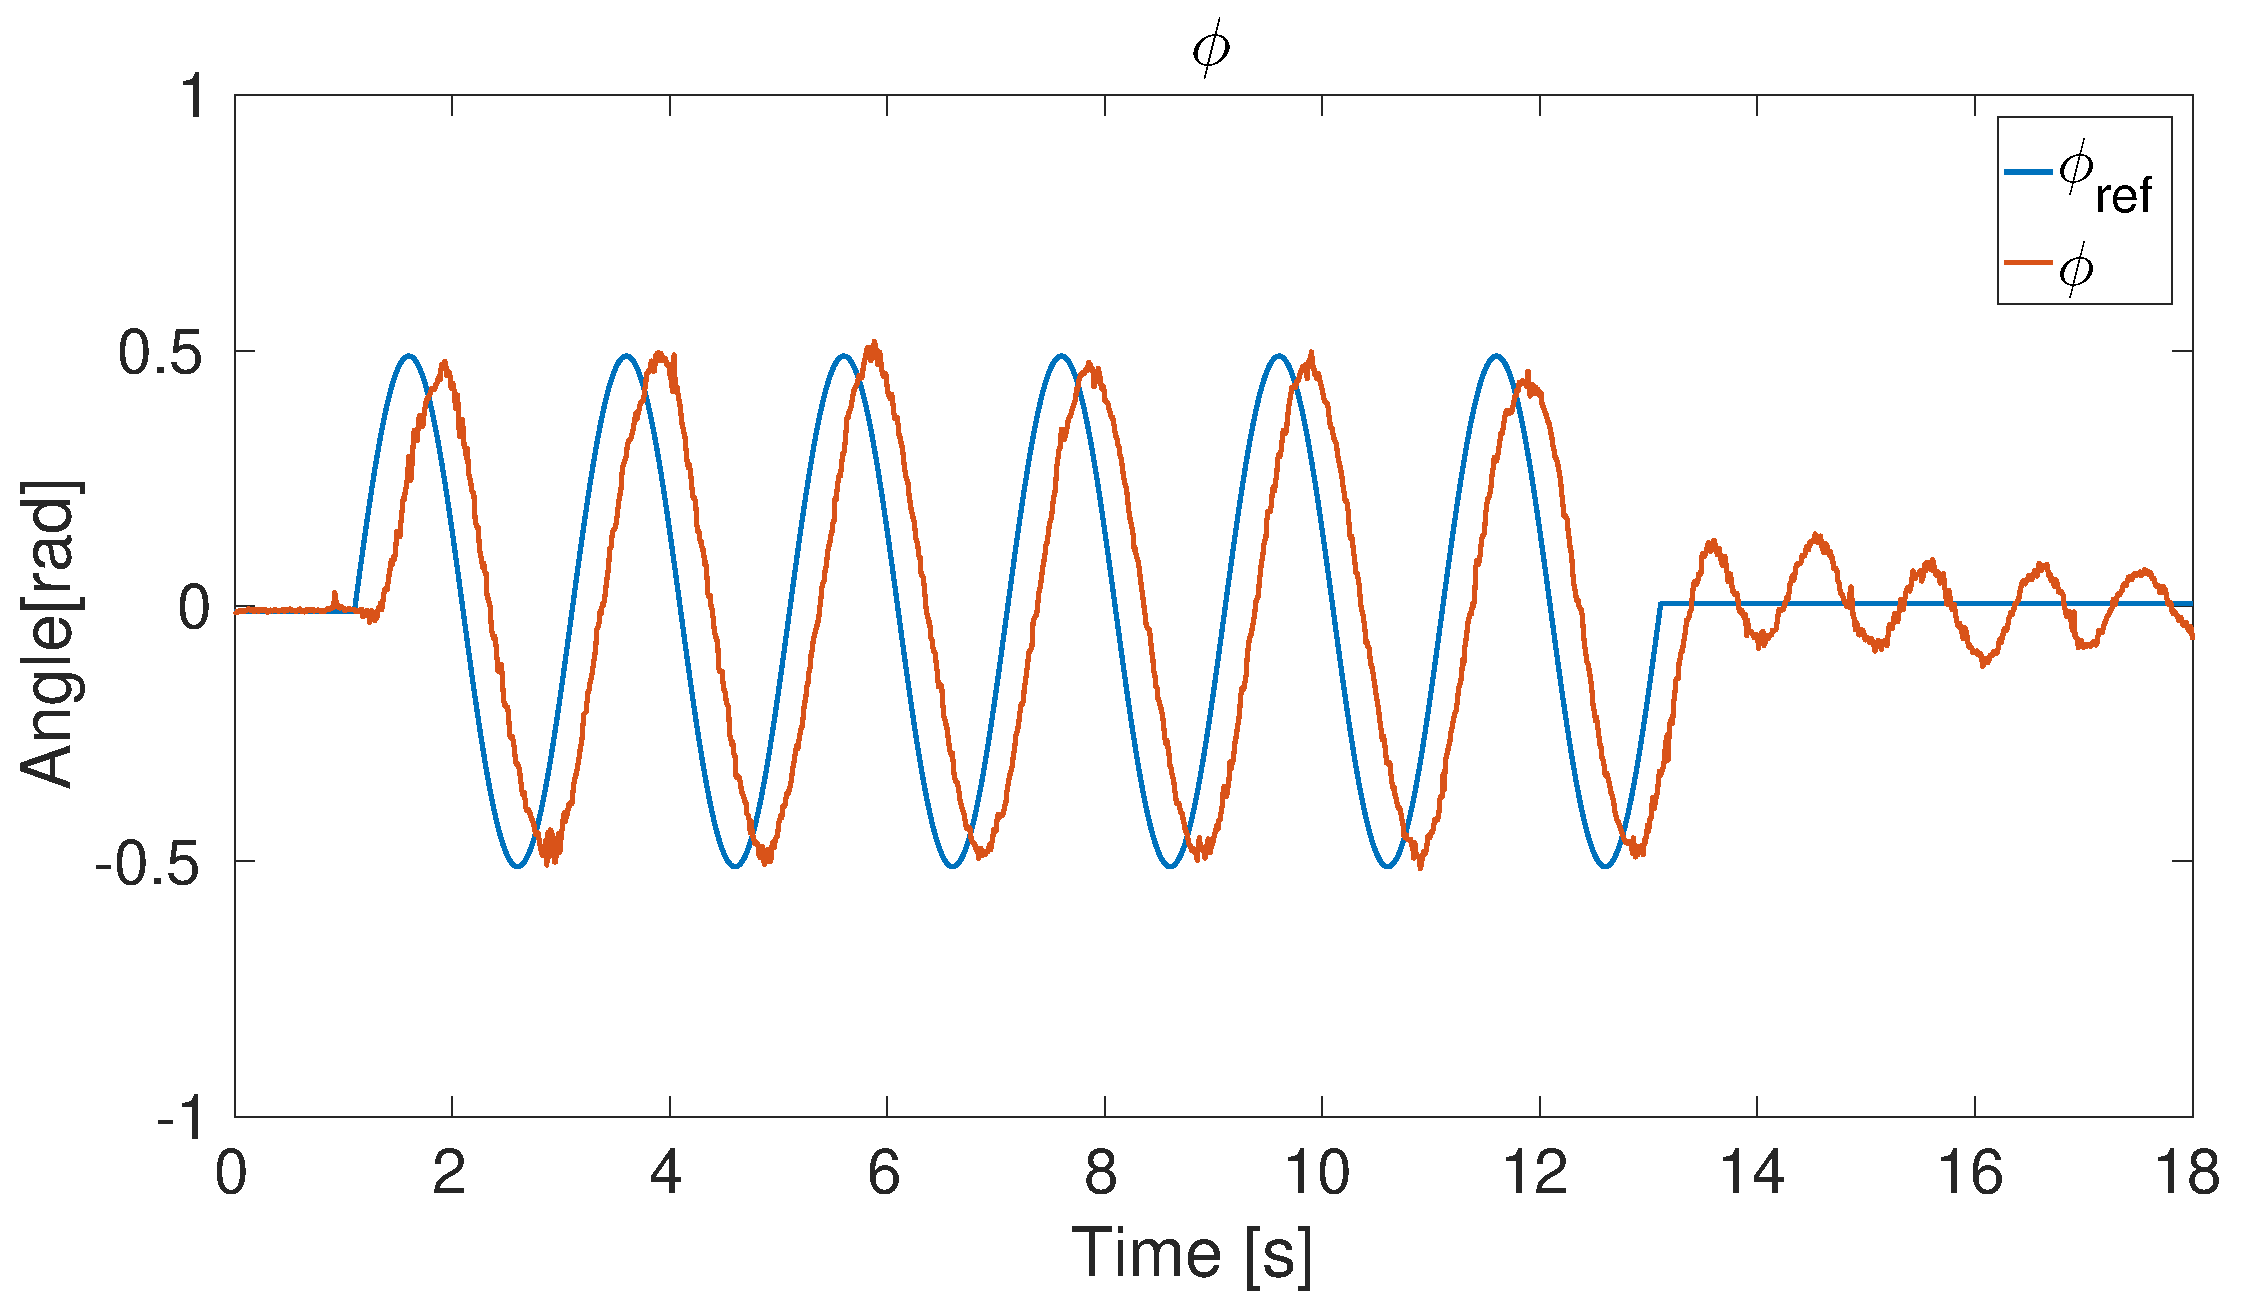
\includegraphics[width=0.4\textwidth]{testSinPhiA05}}
  \qquad
  \subfloat[][\label{fig:AppsimSin05Roll} Simulated response in $\rollAngle$.]{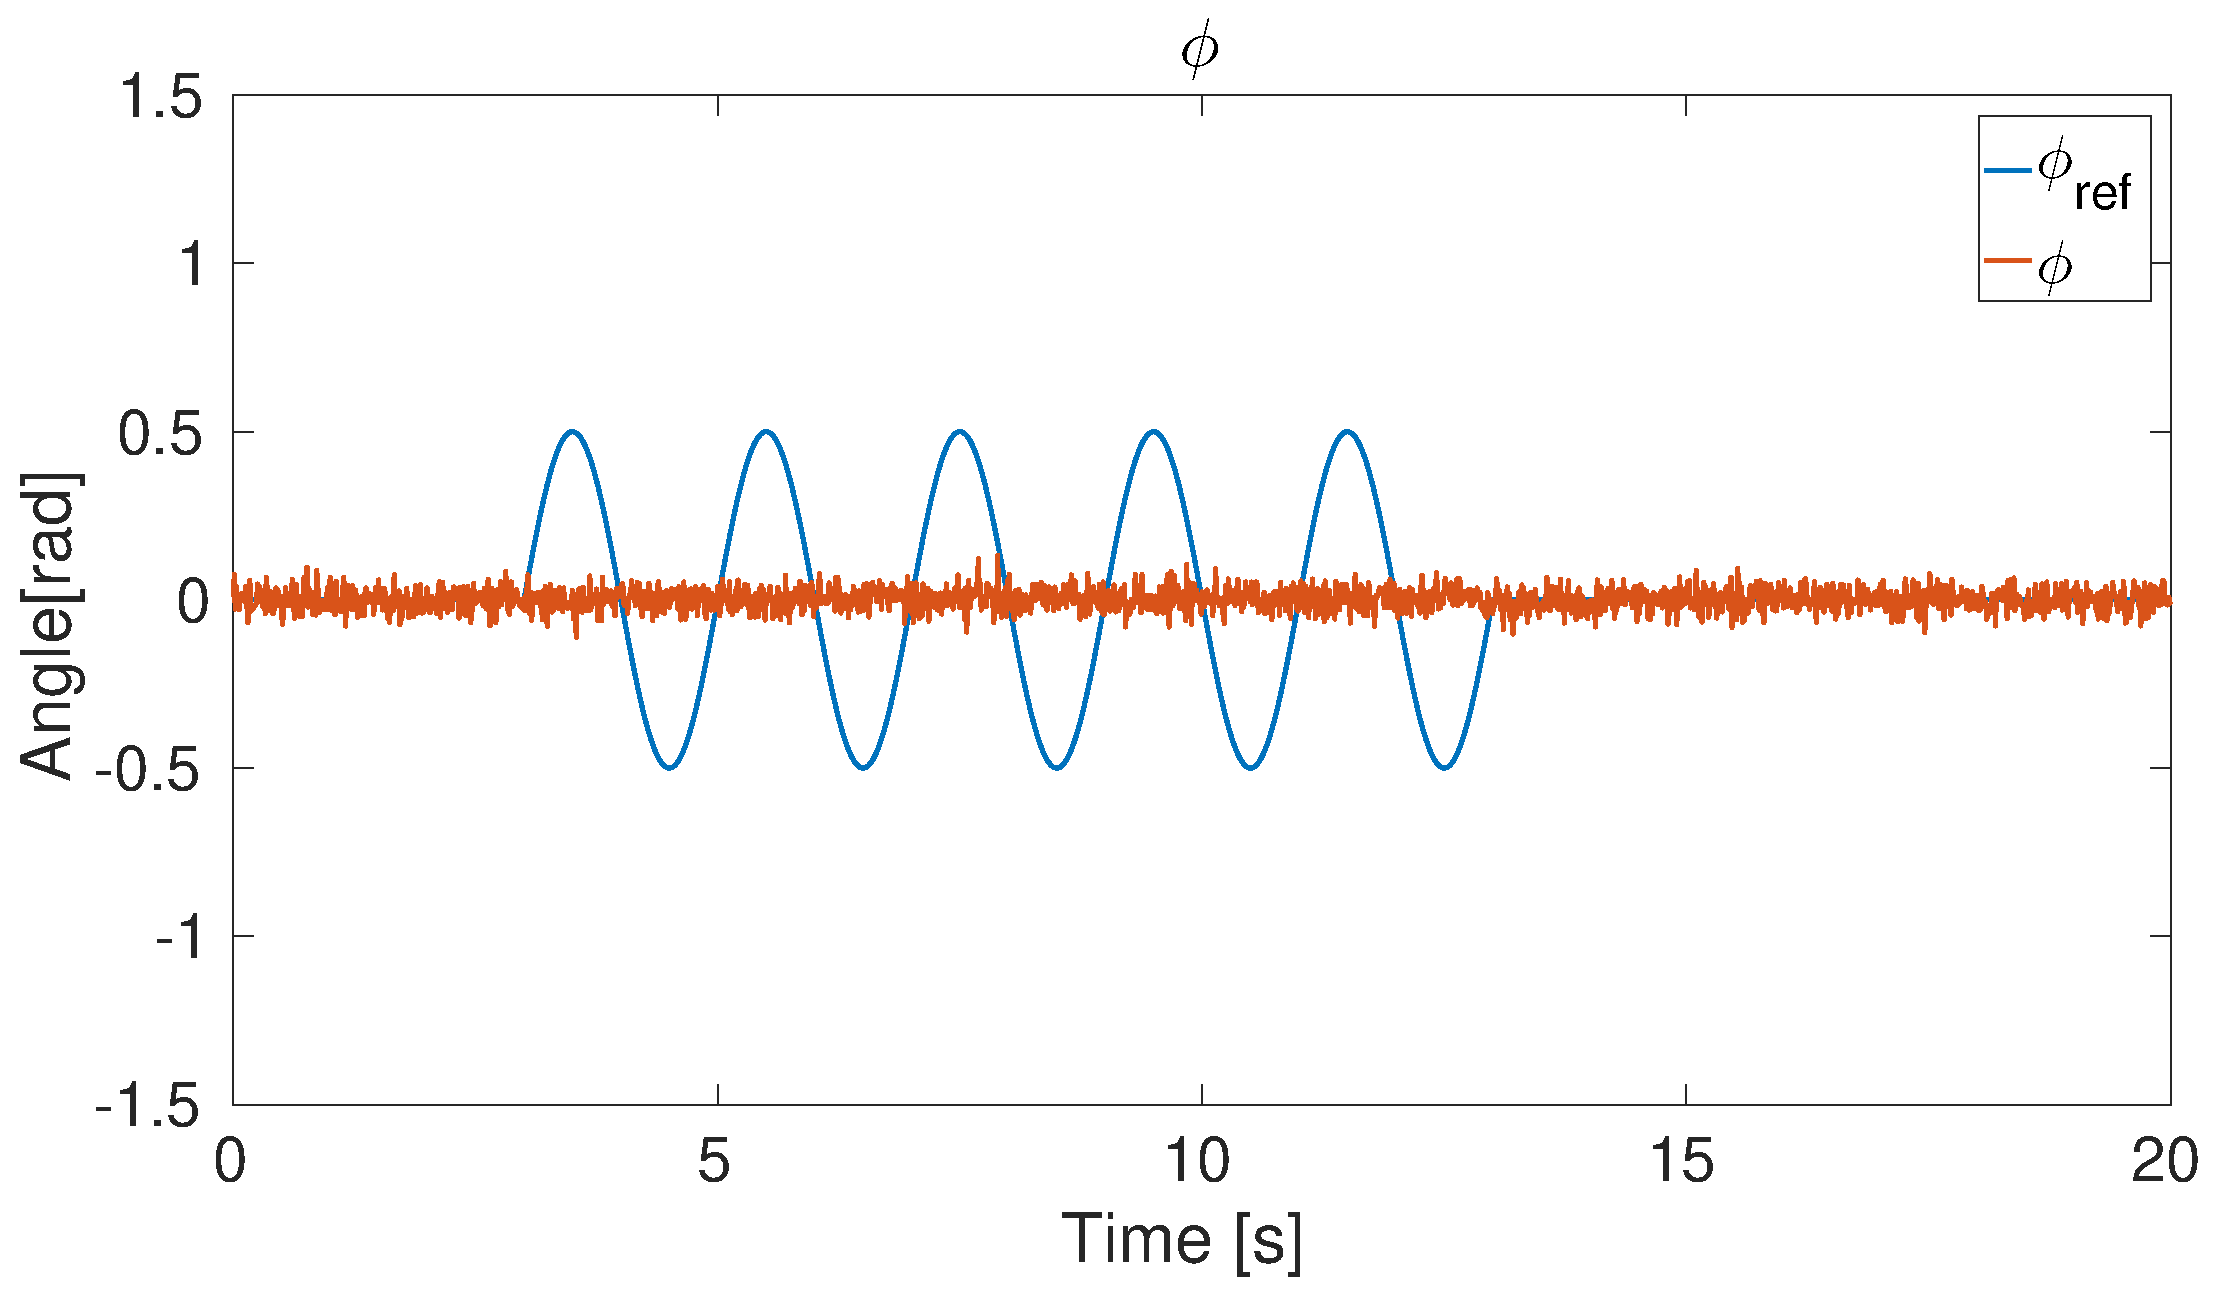
\includegraphics[width=0.4\textwidth]{simSinPhiA05}}
  \qquad
  \subfloat[][\label{fig:ApptestSin05Pitch} Test response in $\pitchAngle$.]{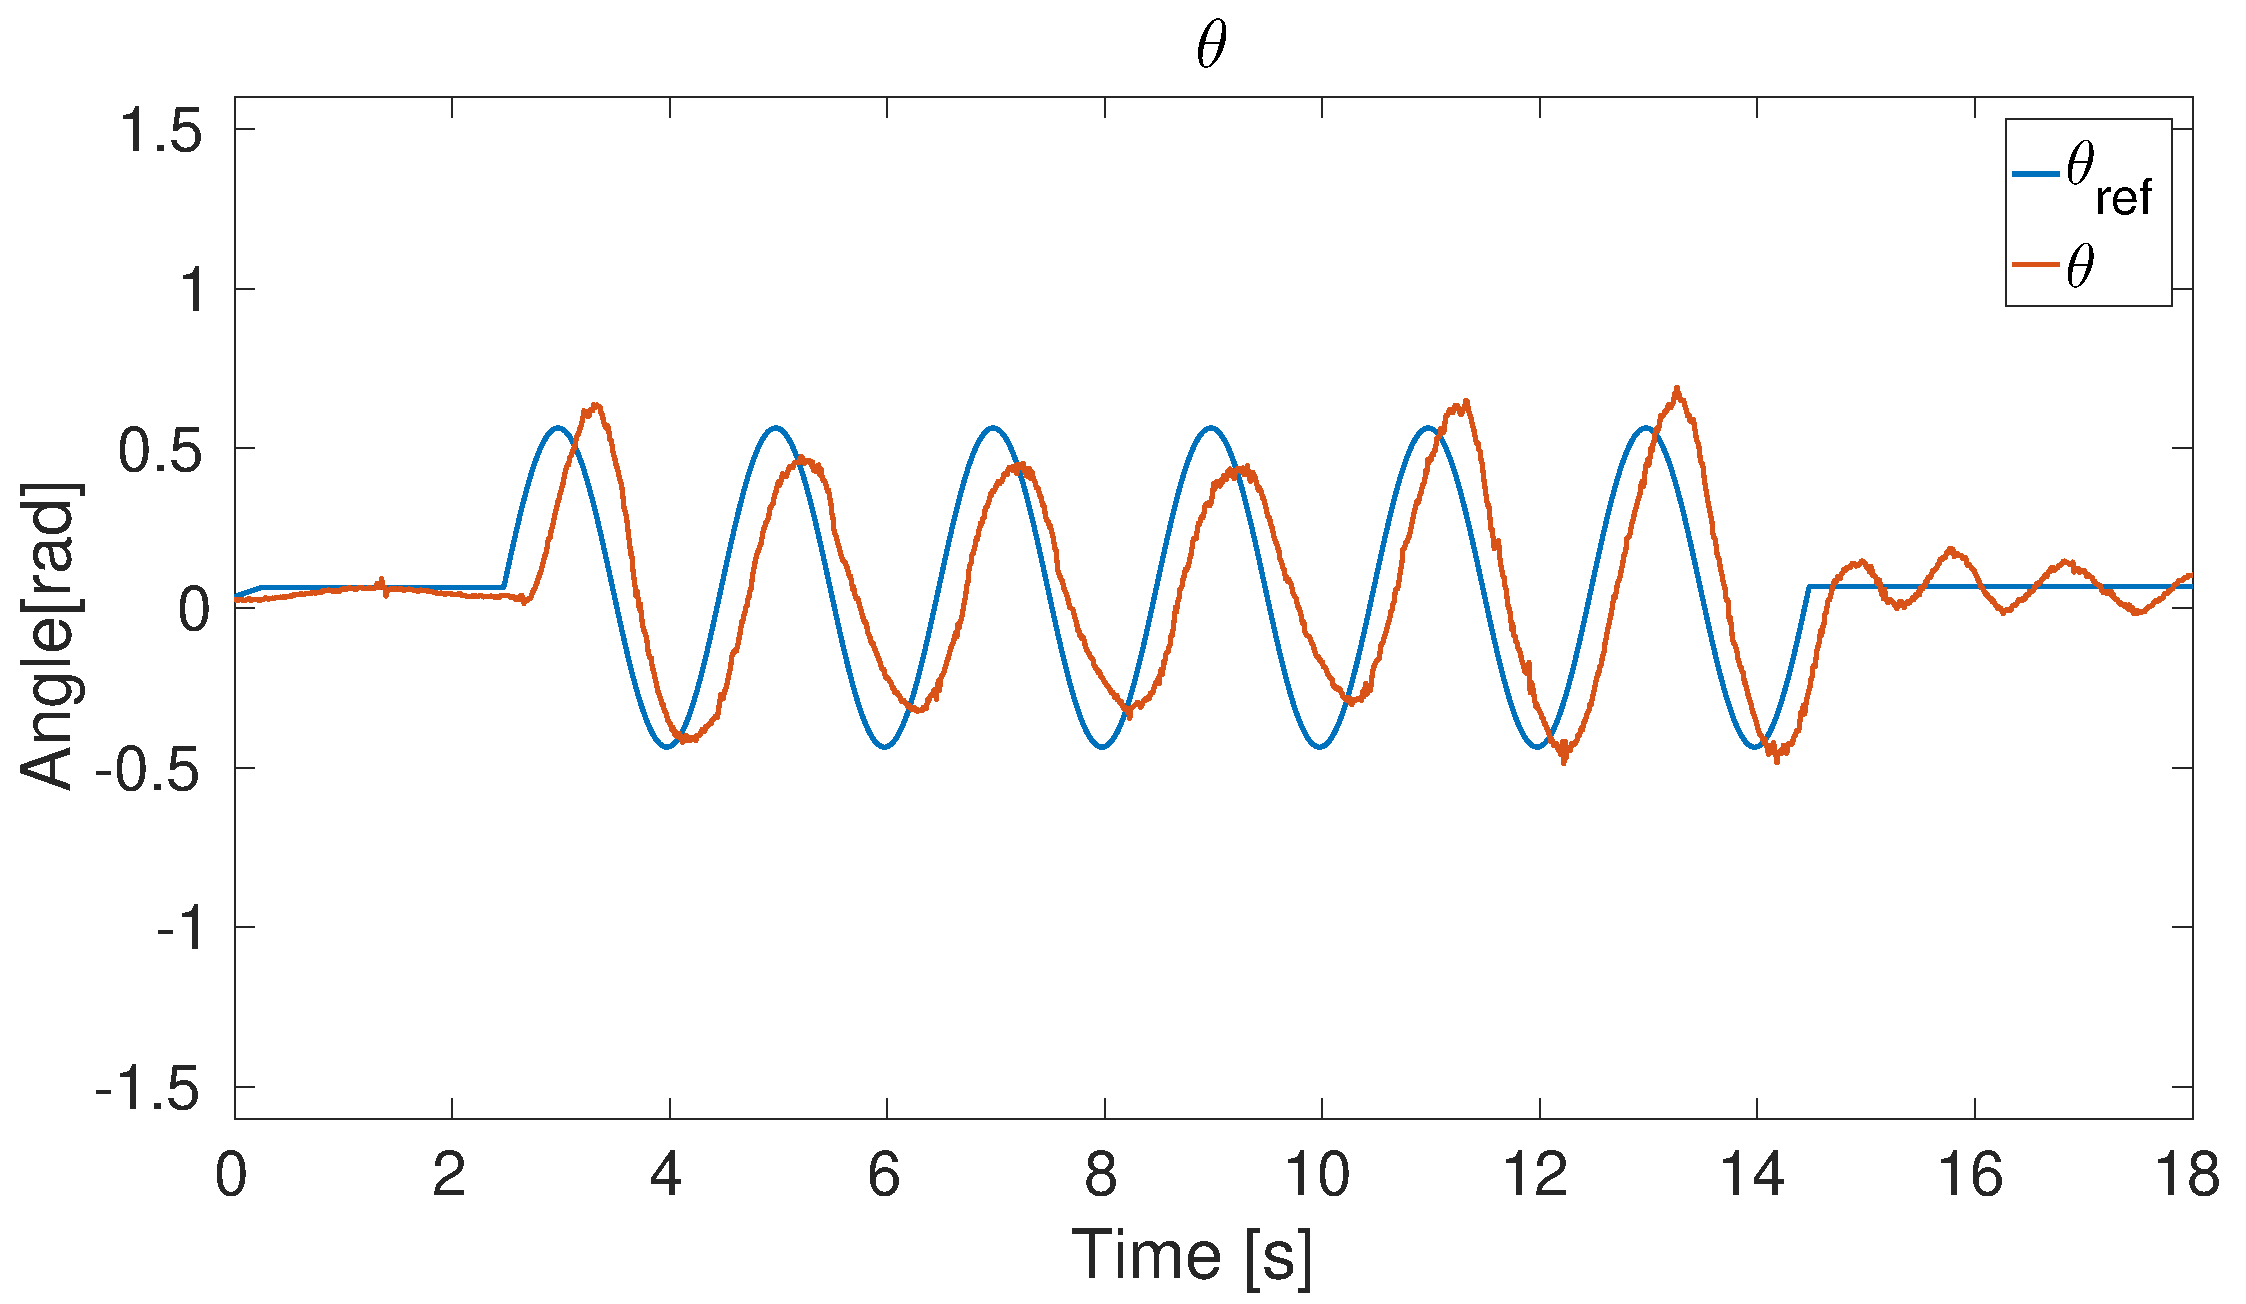
\includegraphics[width=0.4\textwidth]{testSinThetaA05}}
  \qquad
  \subfloat[][\label{fig:AppsimSin05Pitch} Simulated response in $\pitchAngle$.]{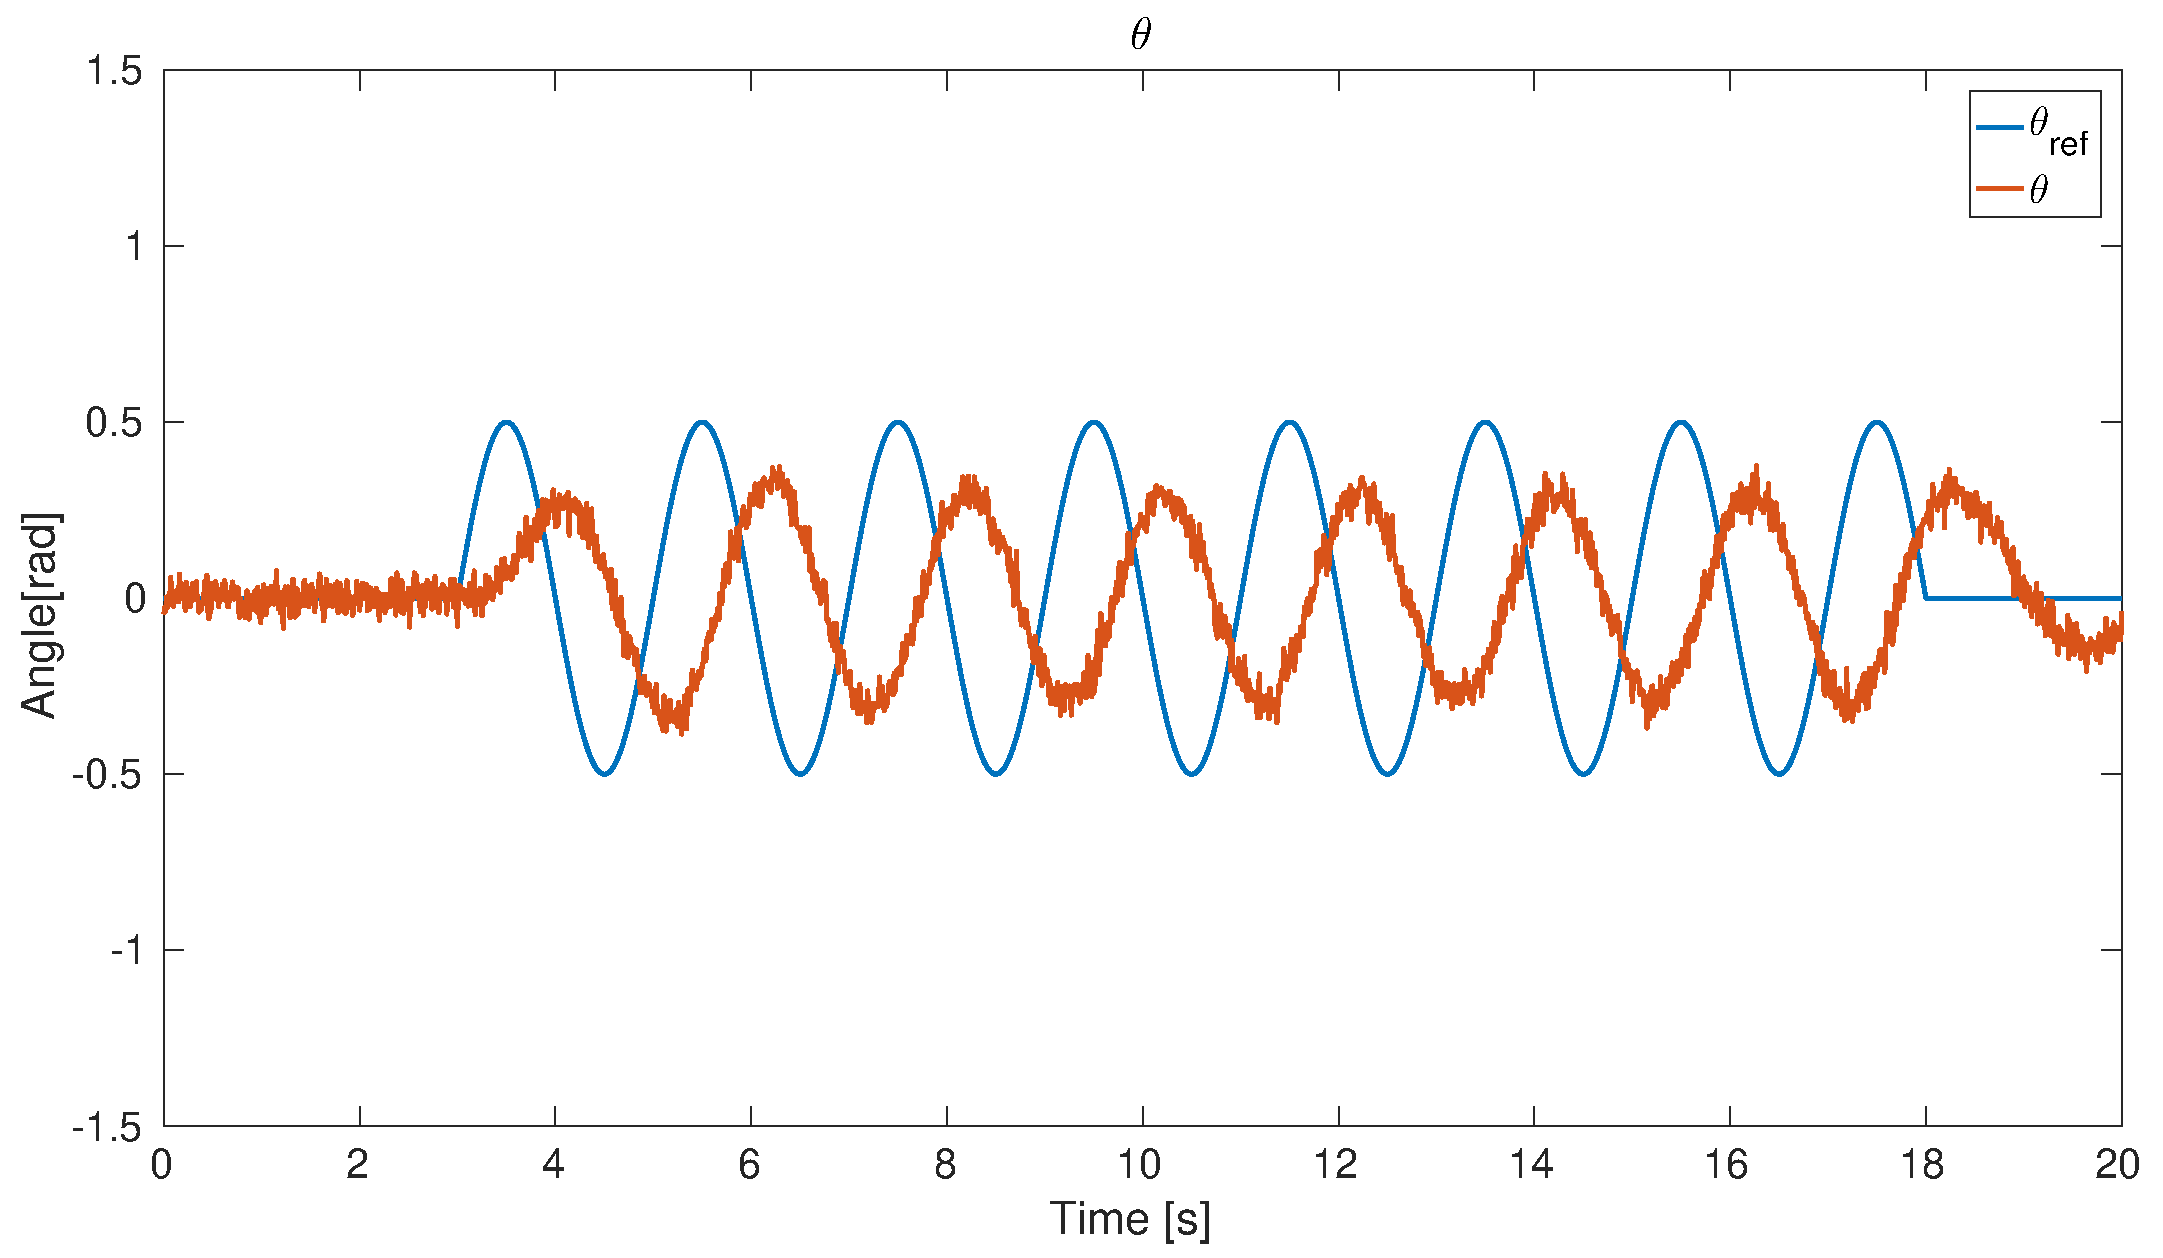
\includegraphics[width=0.4\textwidth]{simSinThetaA05}}
  \qquad
  \subfloat[][\label{fig:ApptestSin05Yaw} Test response in $\yawAngle$.]{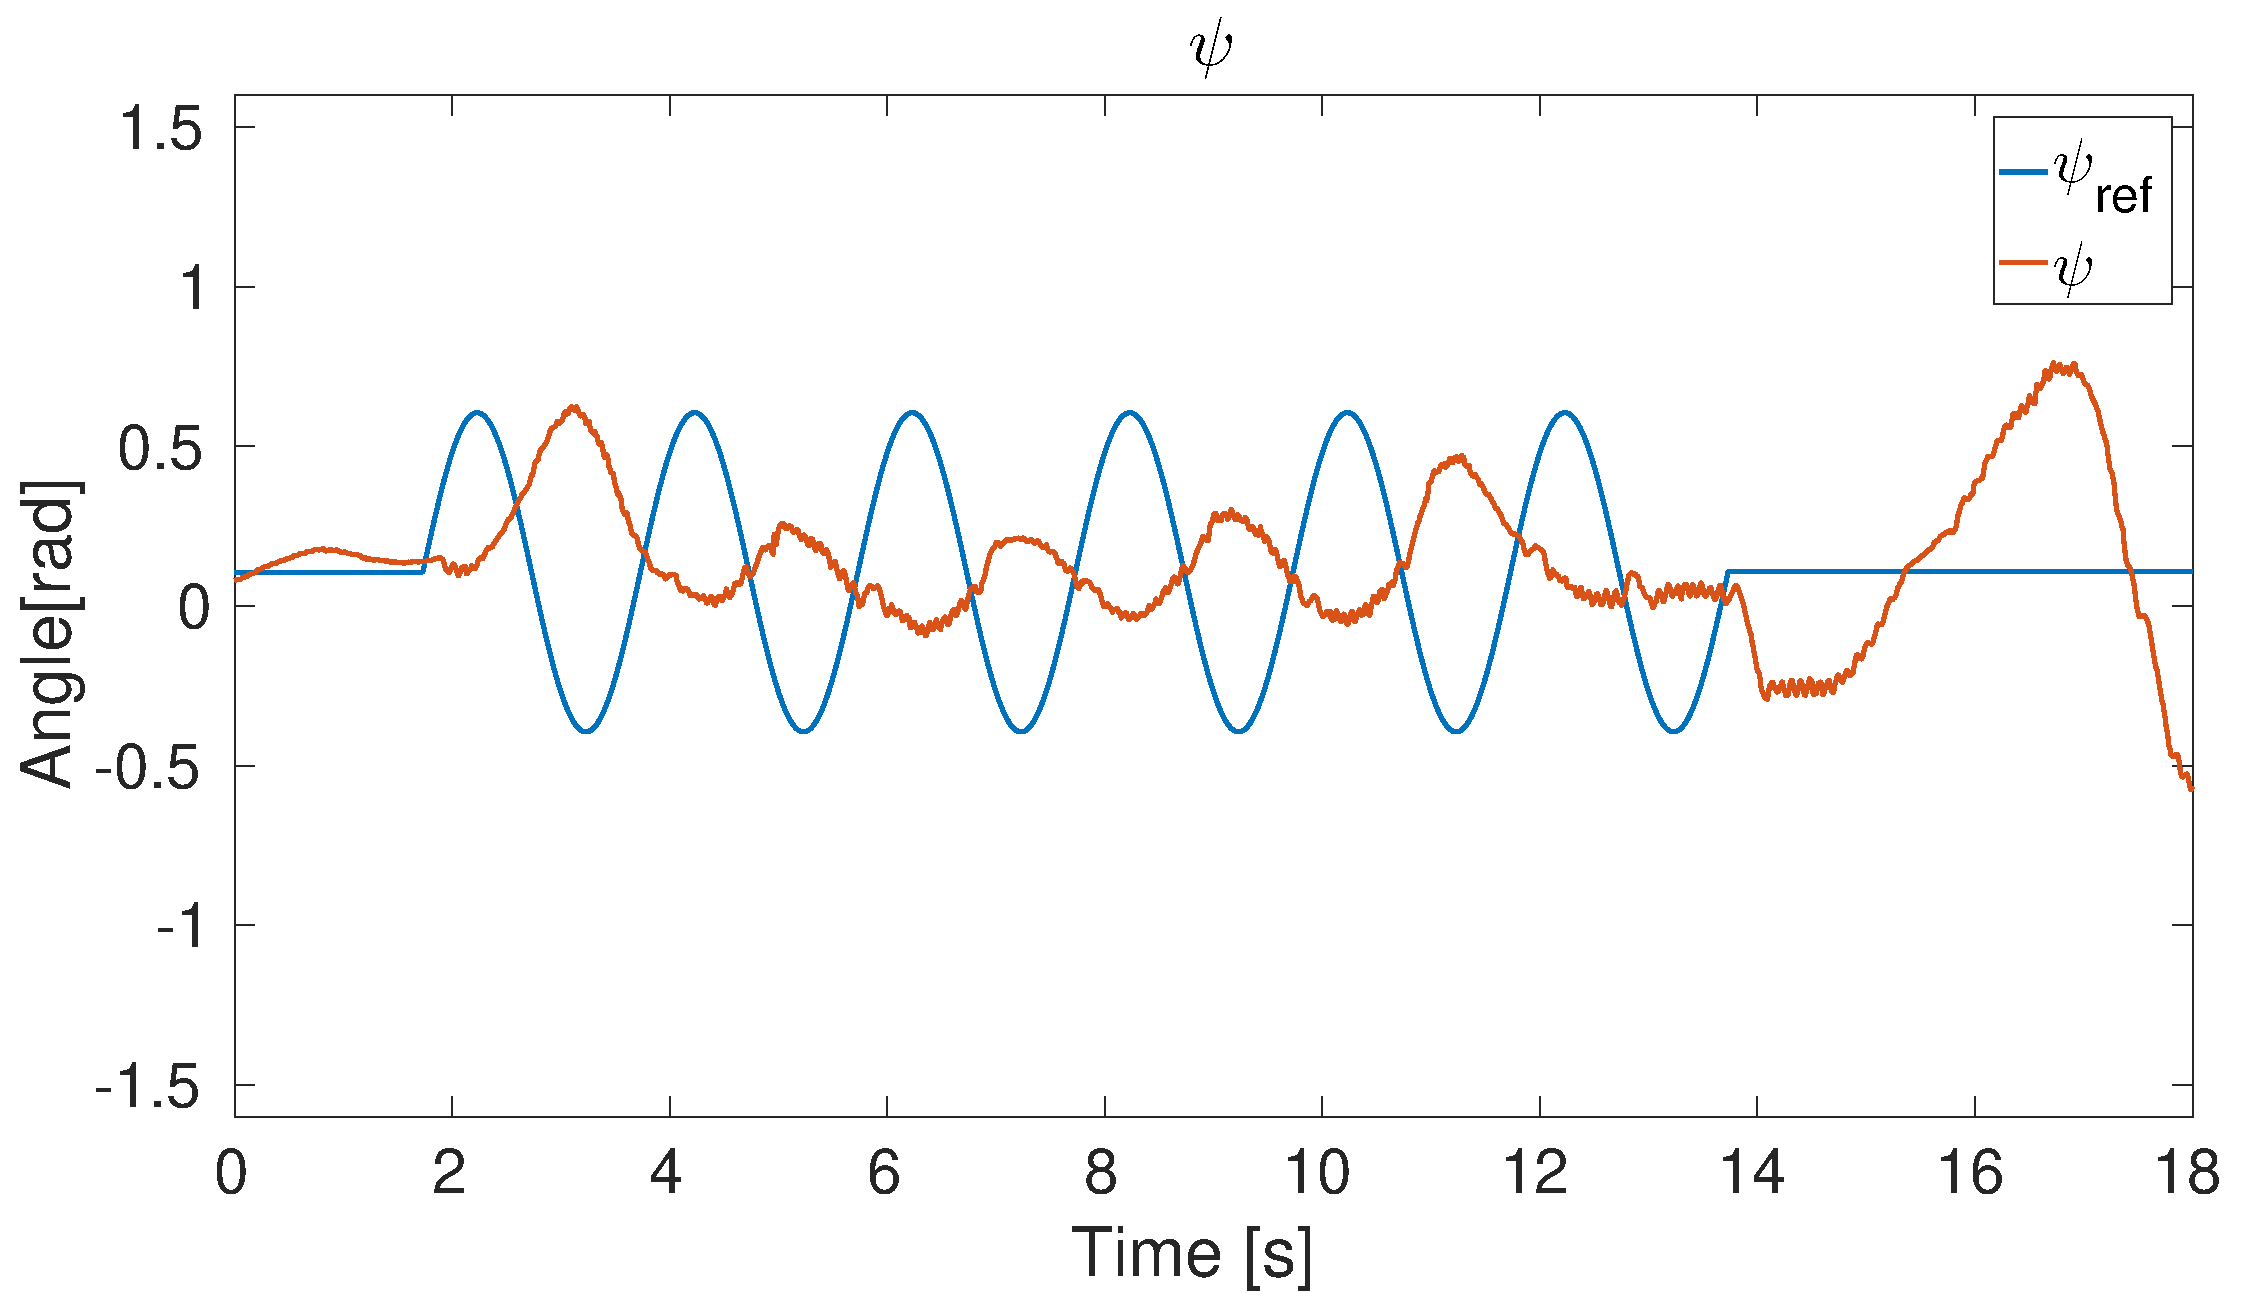
\includegraphics[width=0.4\textwidth]{testSinPsiA05}}
  \qquad
  \subfloat[][\label{fig:AppsimSin50Yaw} Simulated response in $\yawAngle$.]{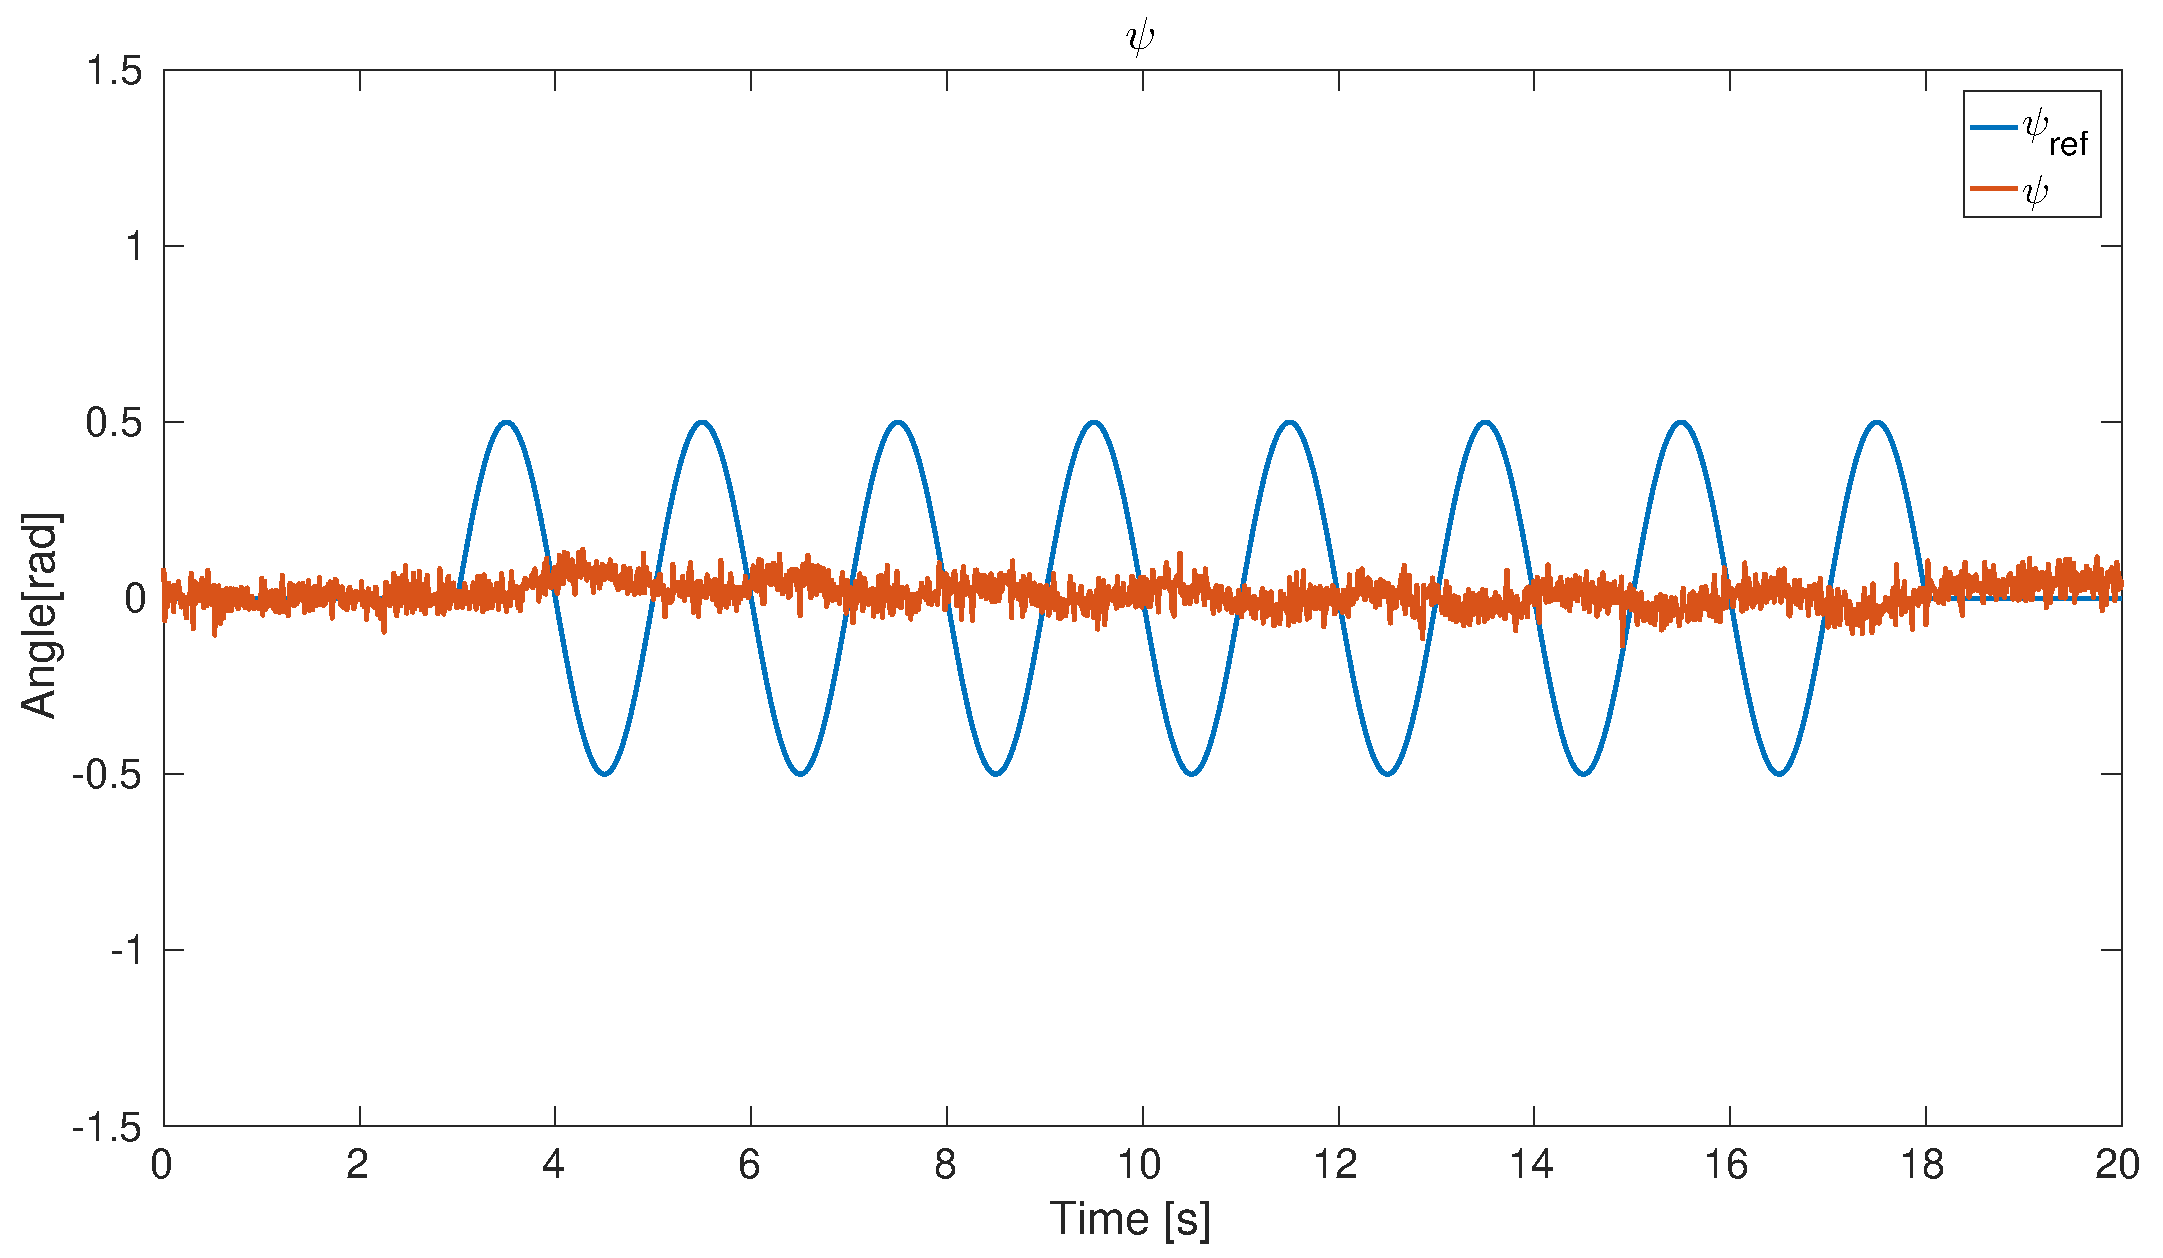
\includegraphics[width=0.4\textwidth]{simSinPsiA05}}
    \caption{\label{fig:AppSin05Attitude}%
   A sine signal with amplitude $0.5$ and frequency $0.5\ \hertz$ was applied in one attitude angle at a time while using the attitude controller. While a sine signal was applied in one attitude angle the other attitude angles were not controlled.}
\end{figure}

\begin{figure}
\centering
  \subfloat[][\label{fig:ApptestSinAll05RollAttitude} Test response in $\rollAngle$.]{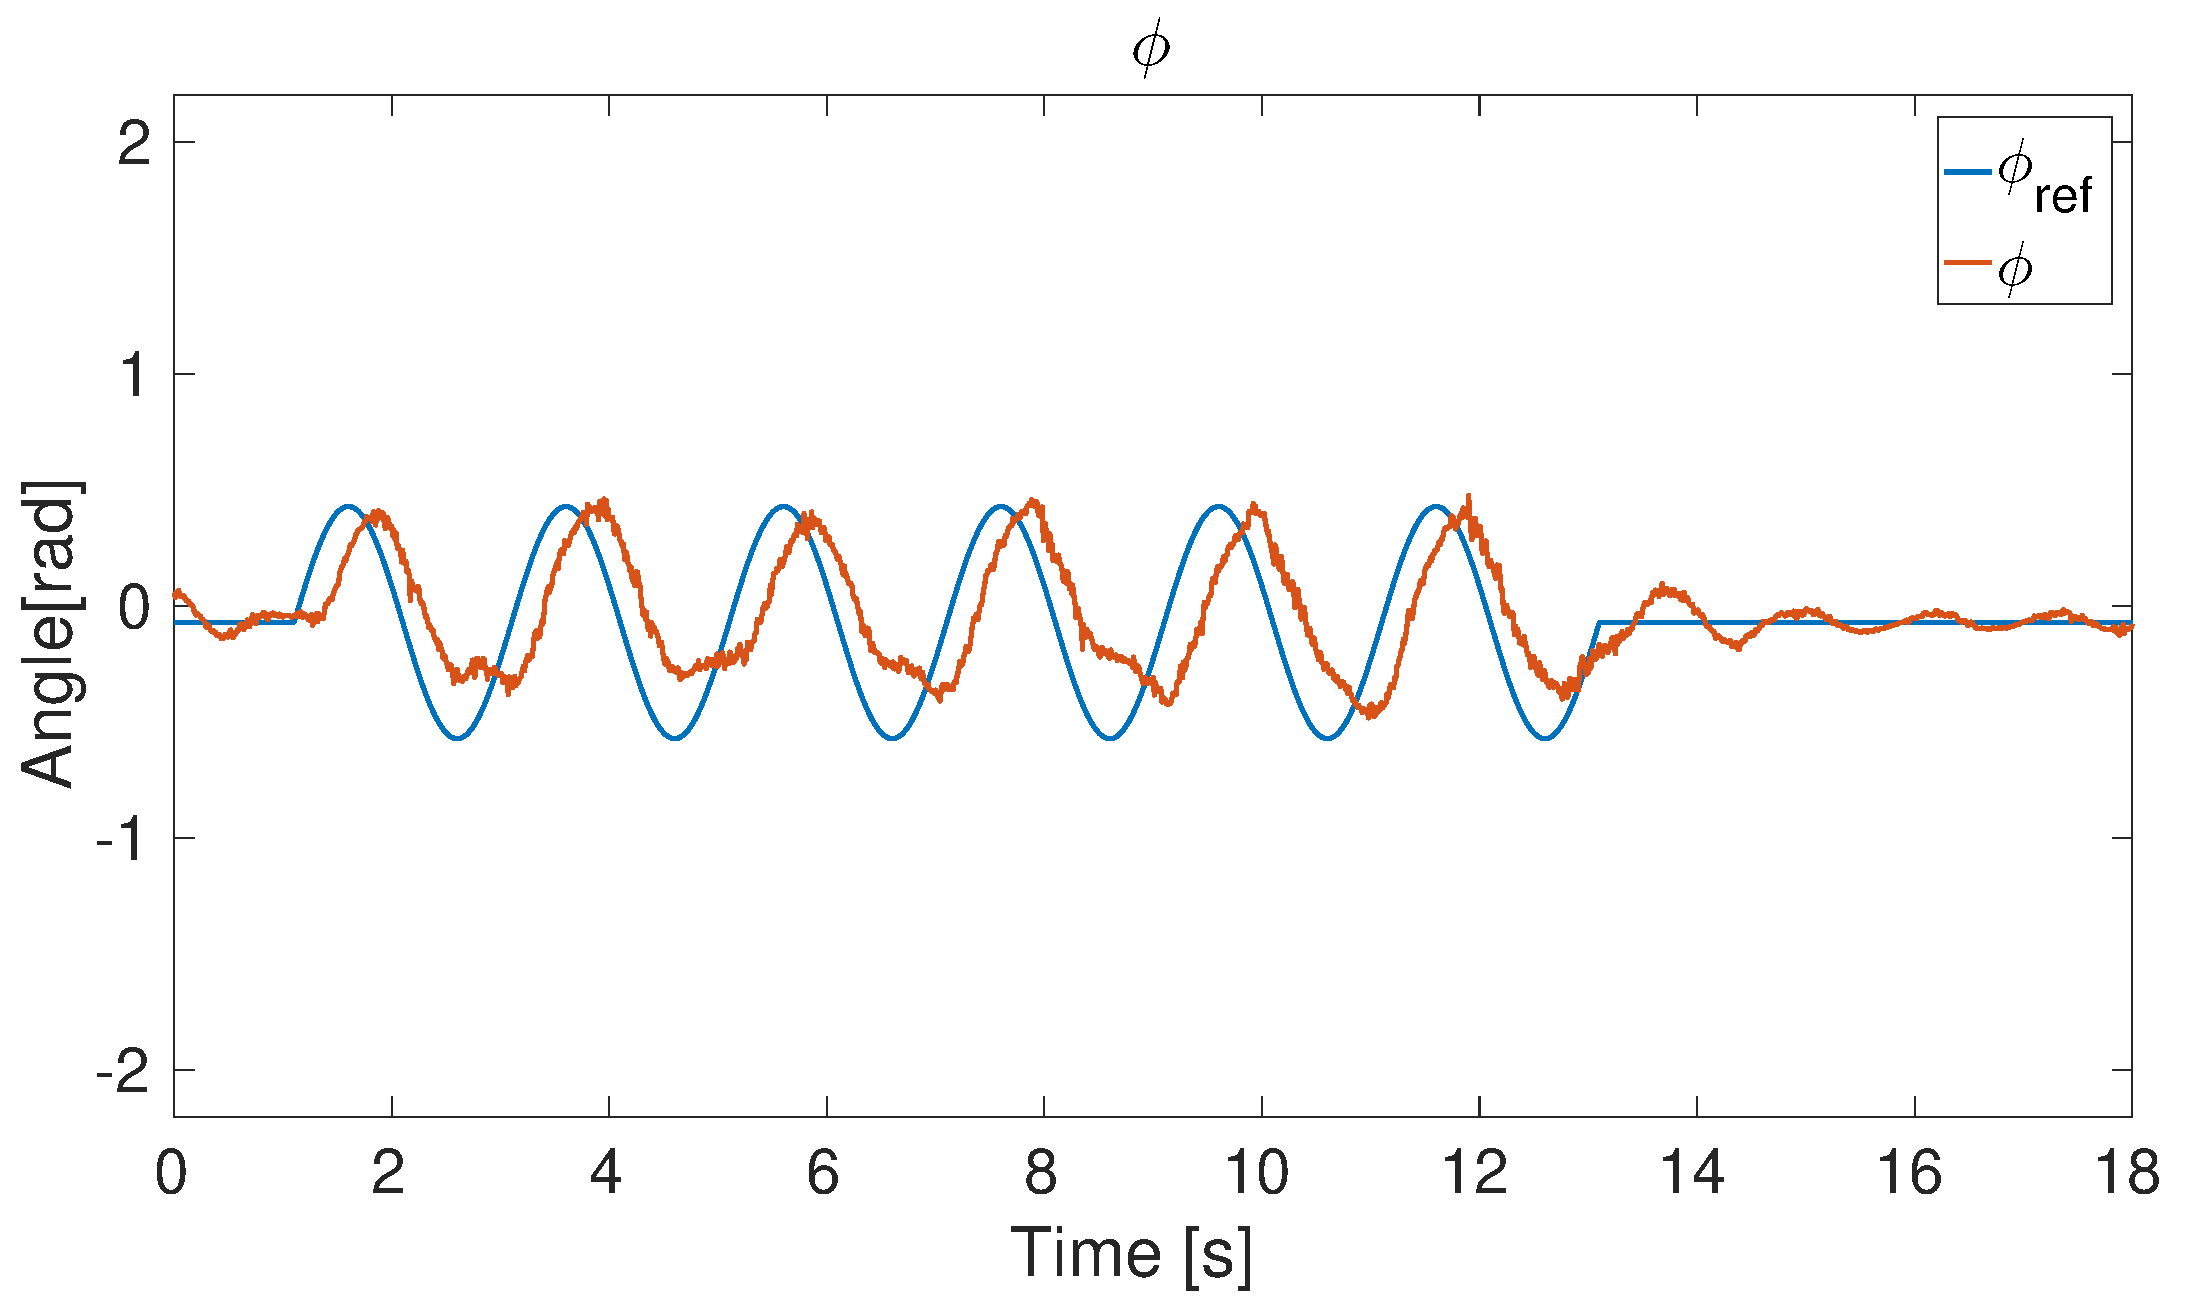
\includegraphics[width=0.4\textwidth]{testSinAllPhiA05}}
  \qquad
  \subfloat[][\label{fig:AppsimSinAll05RollAttitude} Simulated response in $\rollAngle$.]{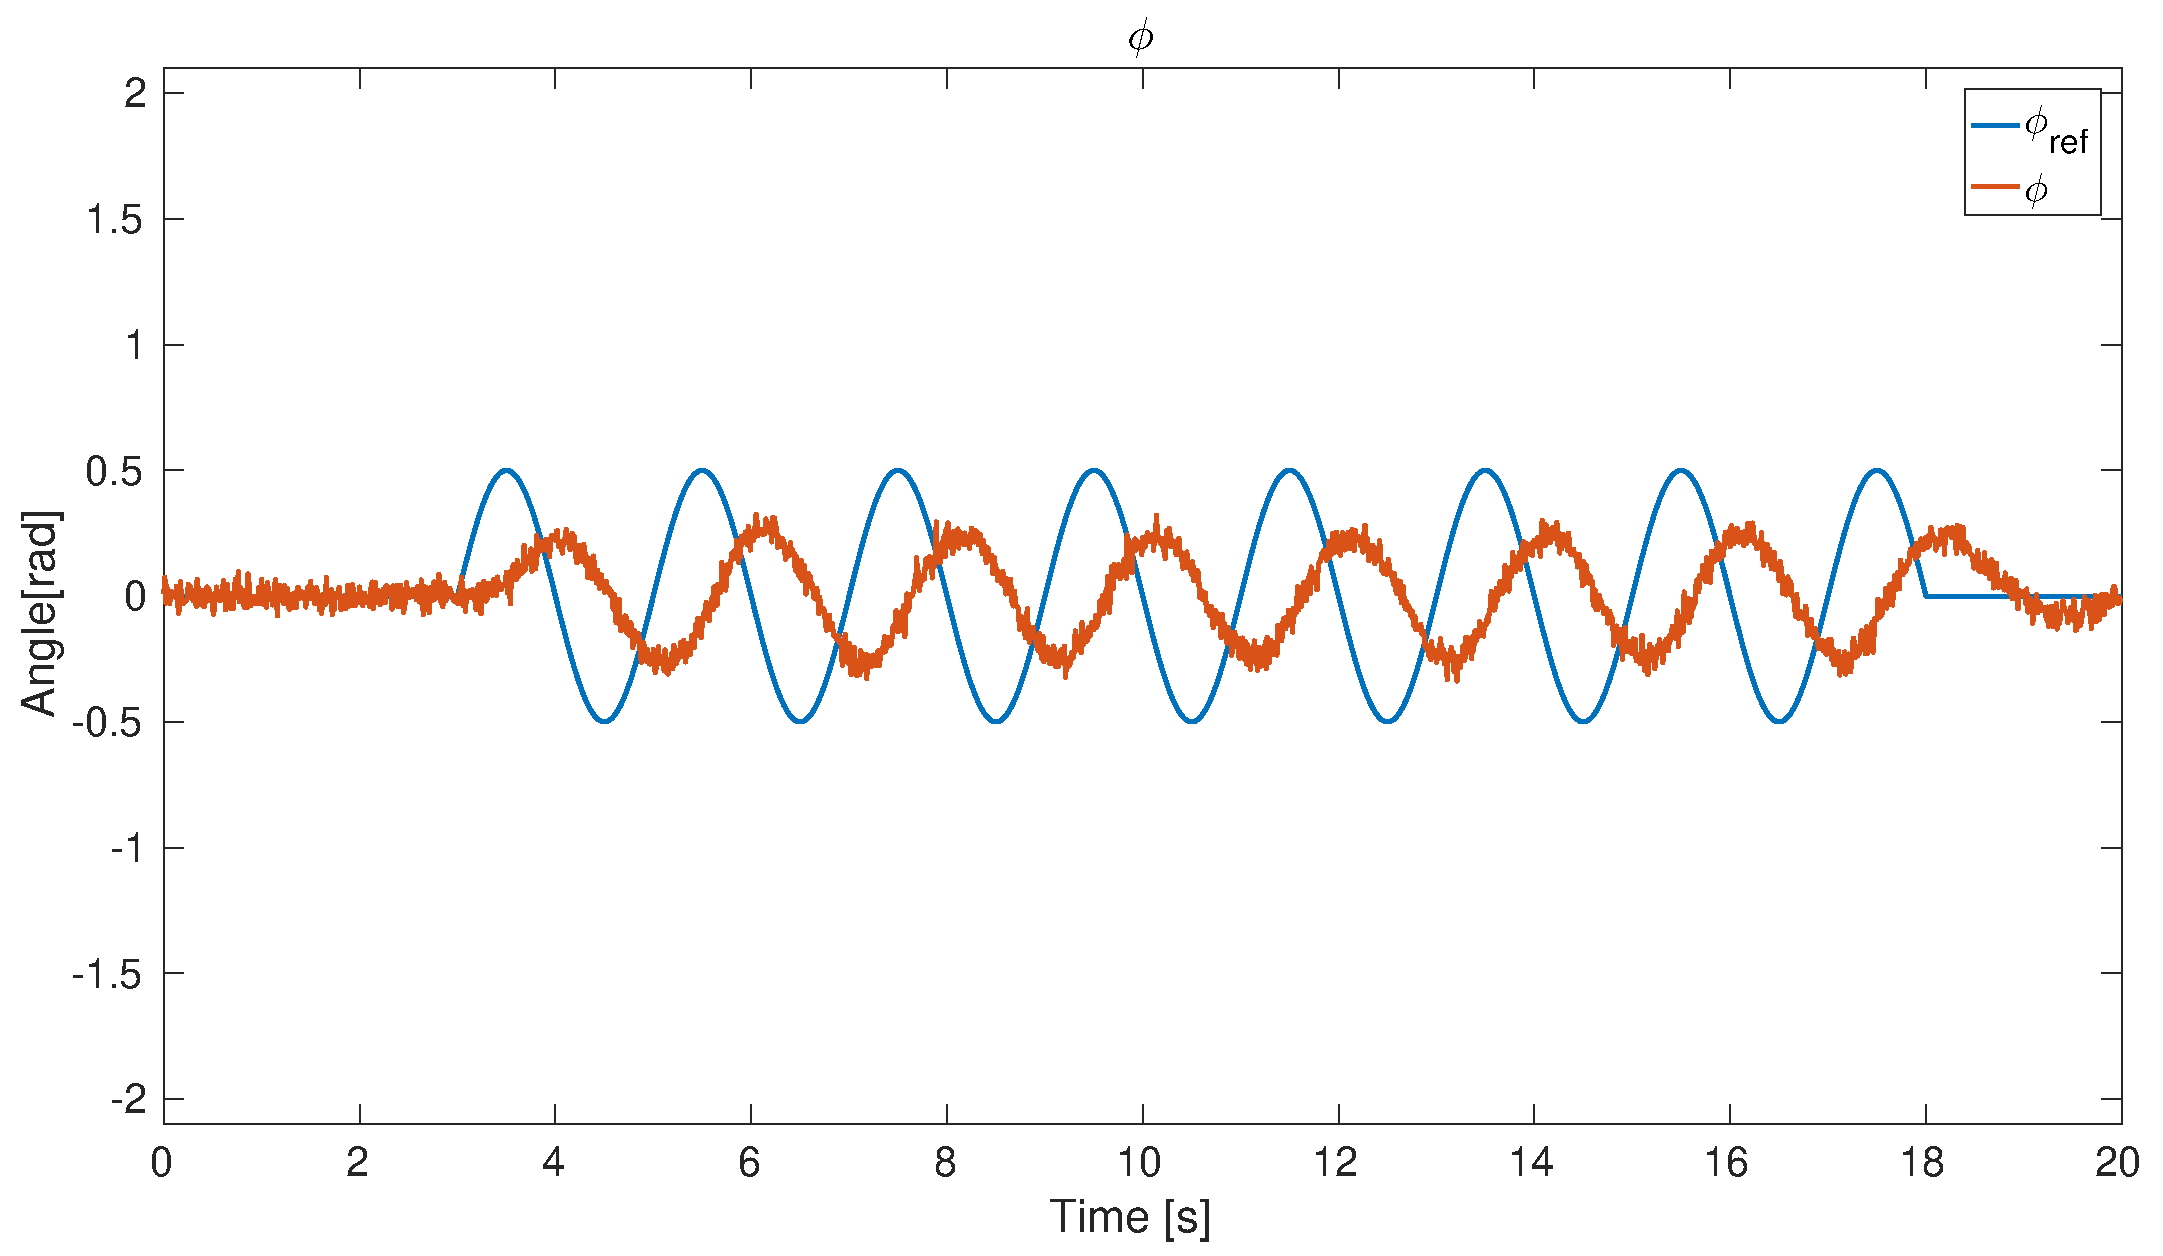
\includegraphics[width=0.4\textwidth]{simSinAllPhiA05}}
  \qquad
  \subfloat[][\label{fig:AppTestSinAll05PitchAttitude}Test response in $\pitchAngle$.]{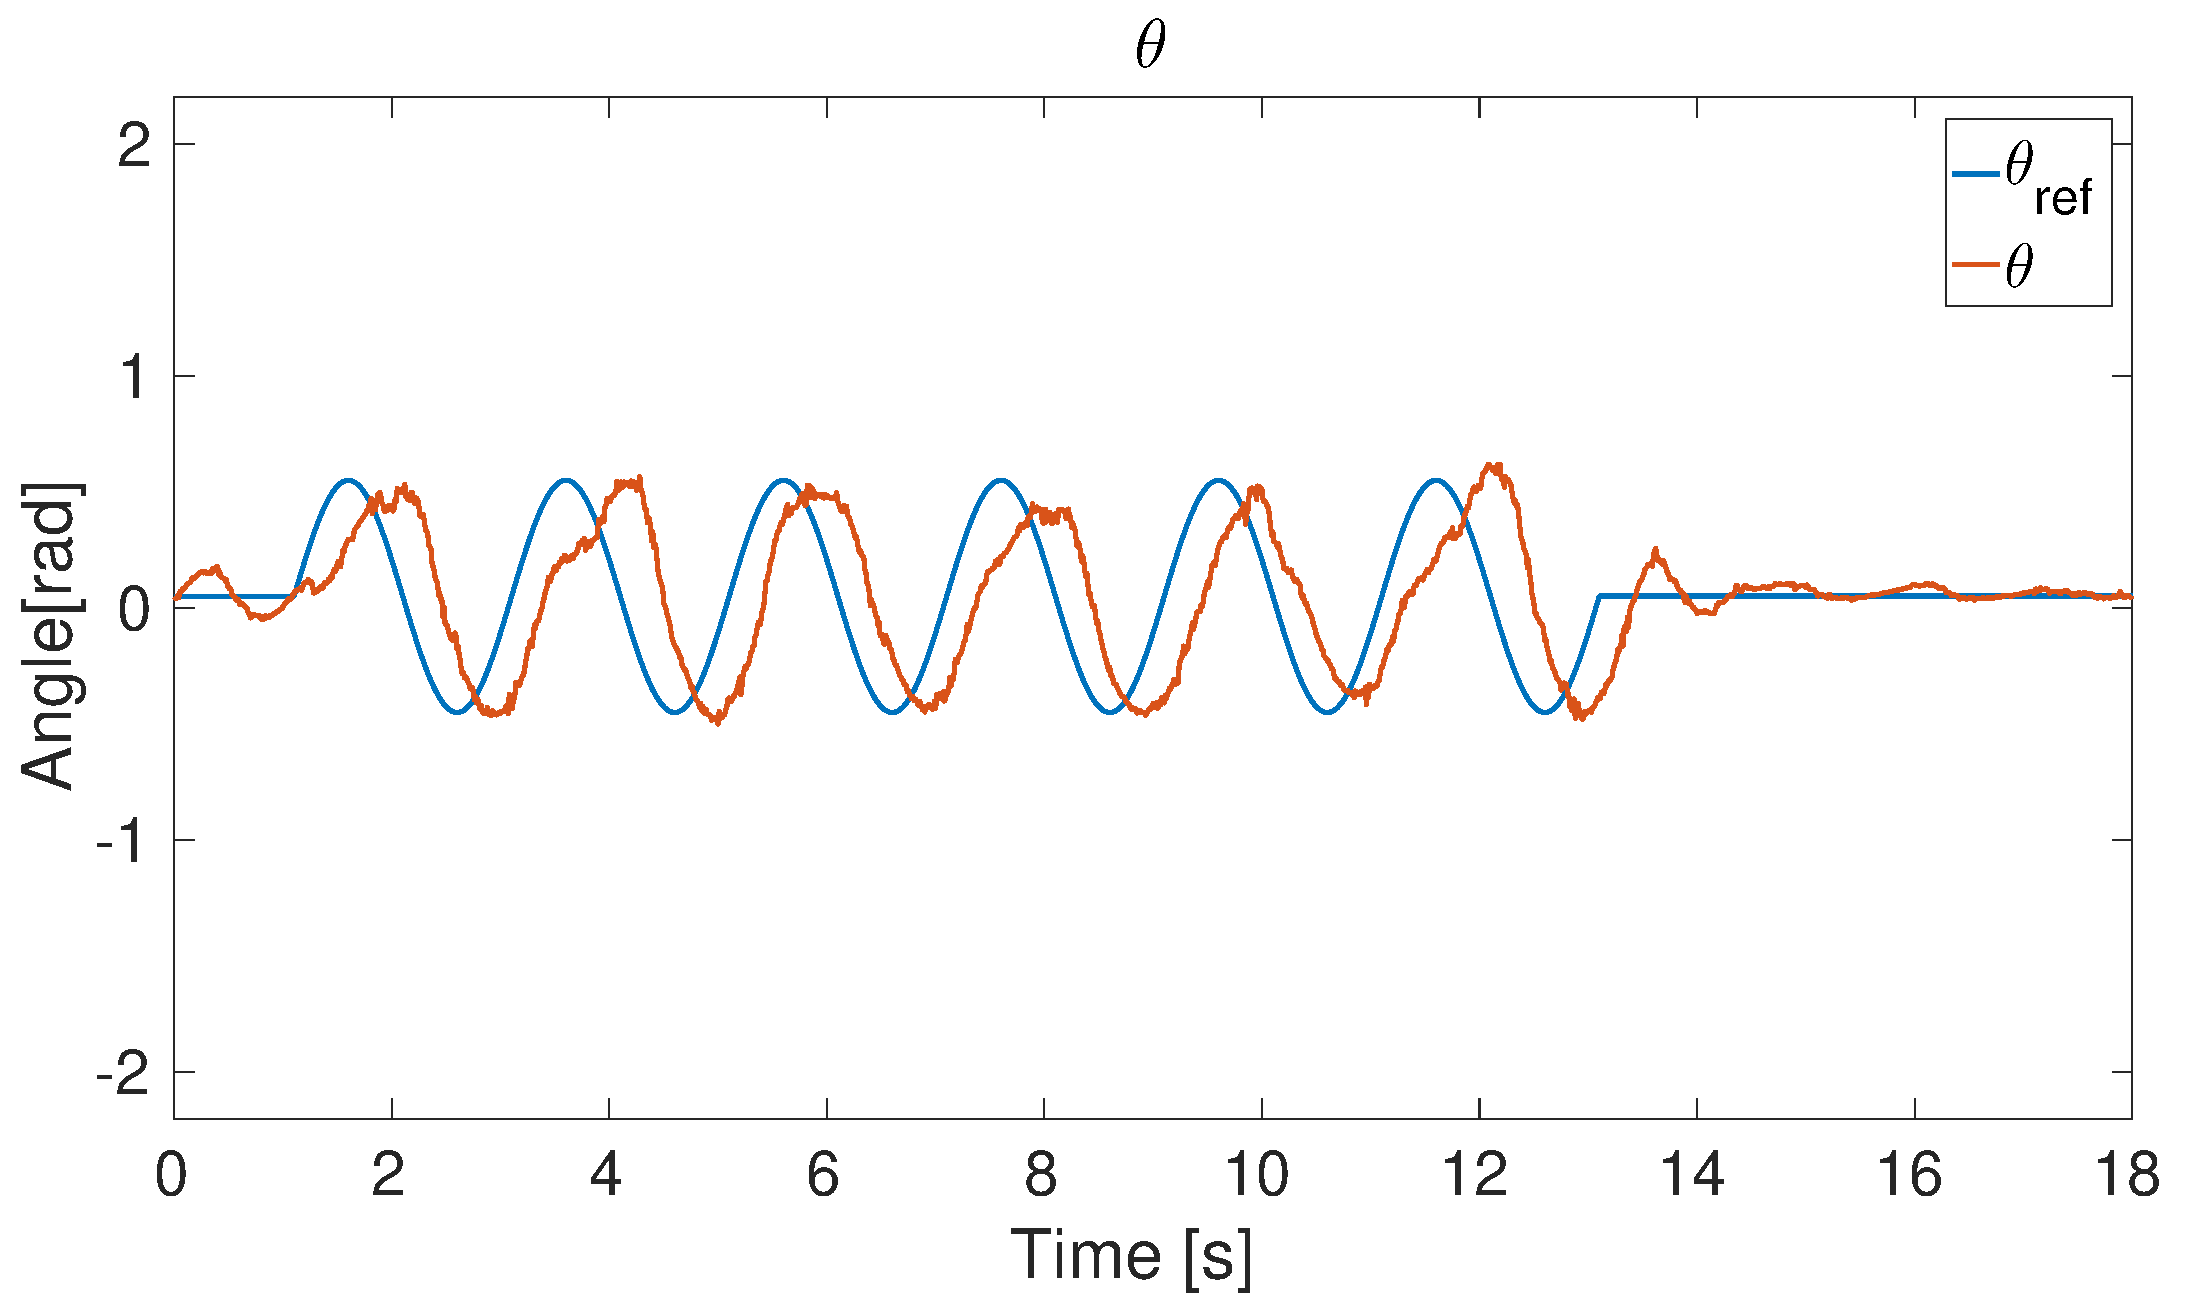
\includegraphics[width=0.4\textwidth]{testSinAllThetaA05}}
  \qquad
  \subfloat[][\label{fig:AppsimSinAll05PitchAttitude} Simulated response in $\pitchAngle$.]{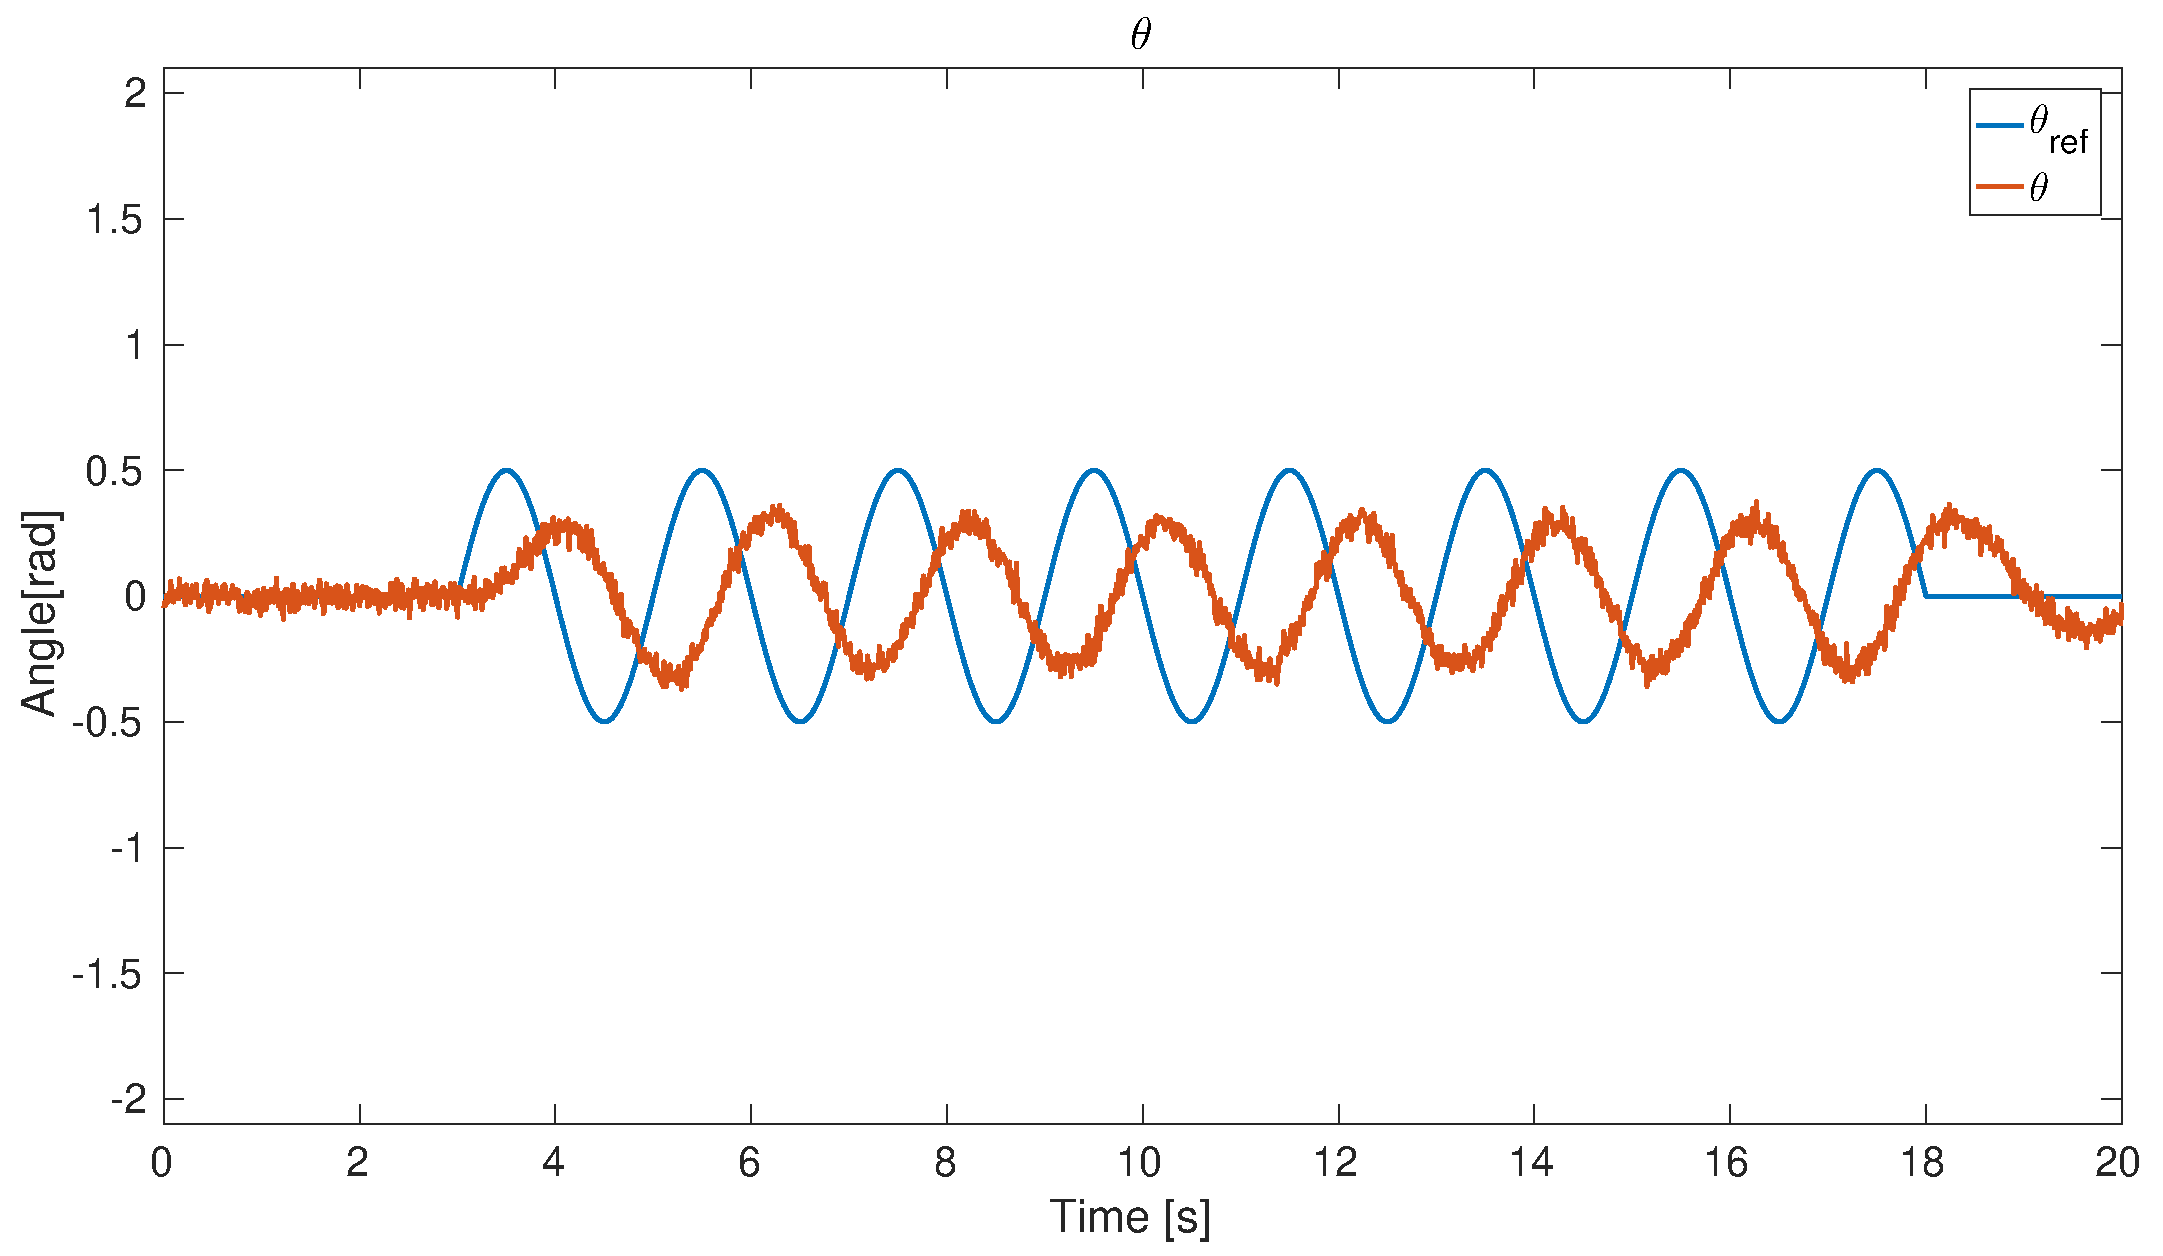
\includegraphics[width=0.4\textwidth]{simSinAllThetaA05}}
  \qquad
  \subfloat[][\label{fig:AppTestSinAll05YawAttitude} Test response in $\yawAngle$.]{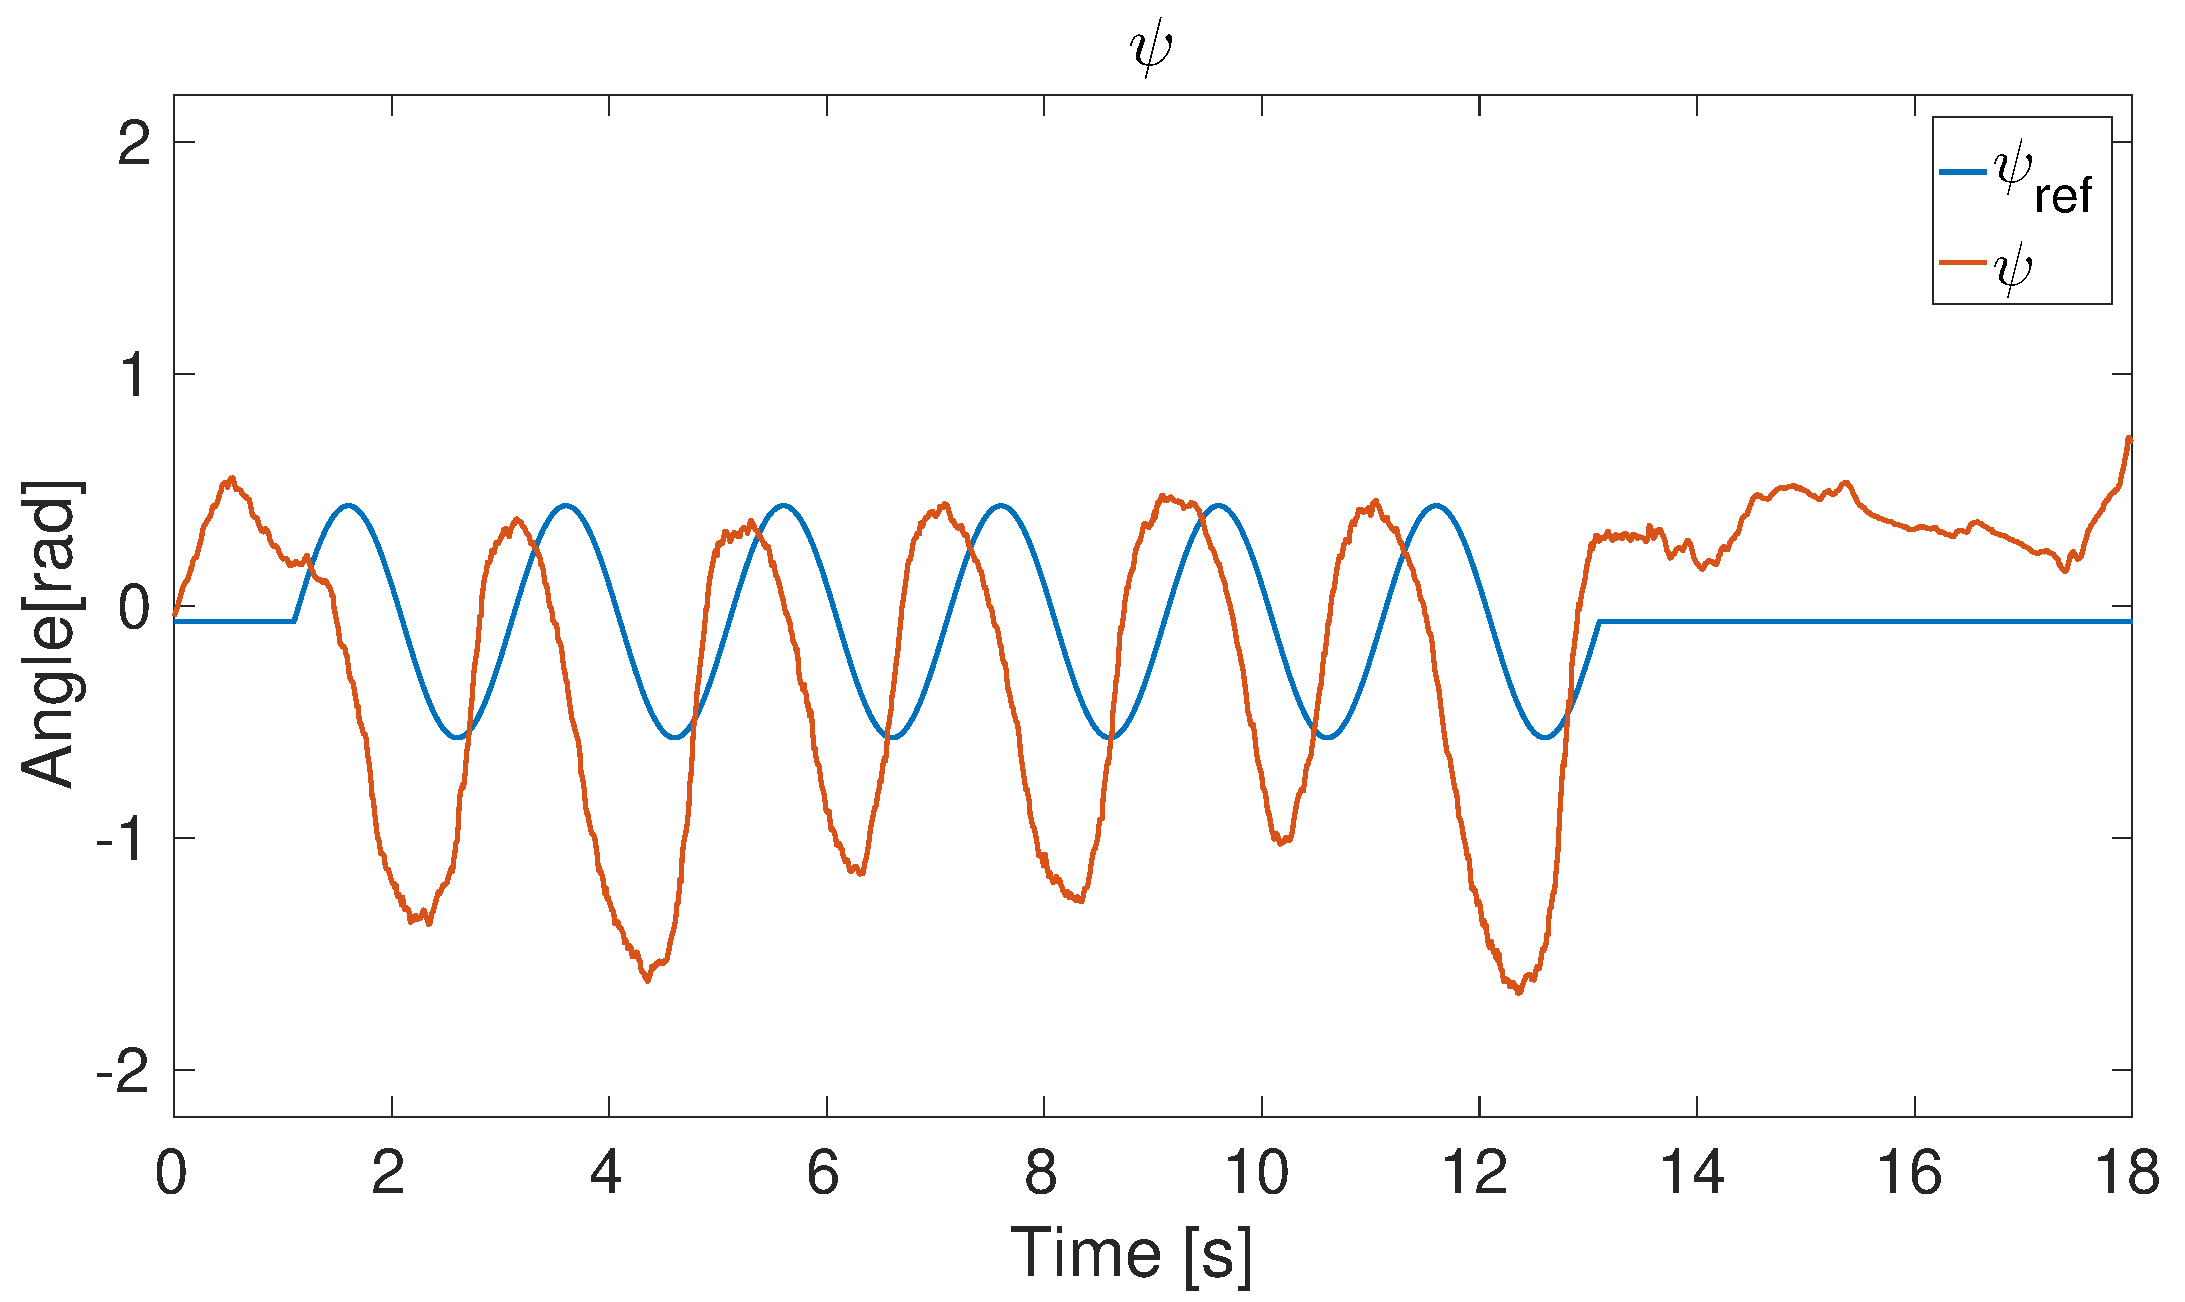
\includegraphics[width=0.4\textwidth]{testSinAllPsiA05}}
  \qquad
  \subfloat[][\label{fig:AppsimSinAll05YawAttitude} Simulated response in $\yawAngle$.]{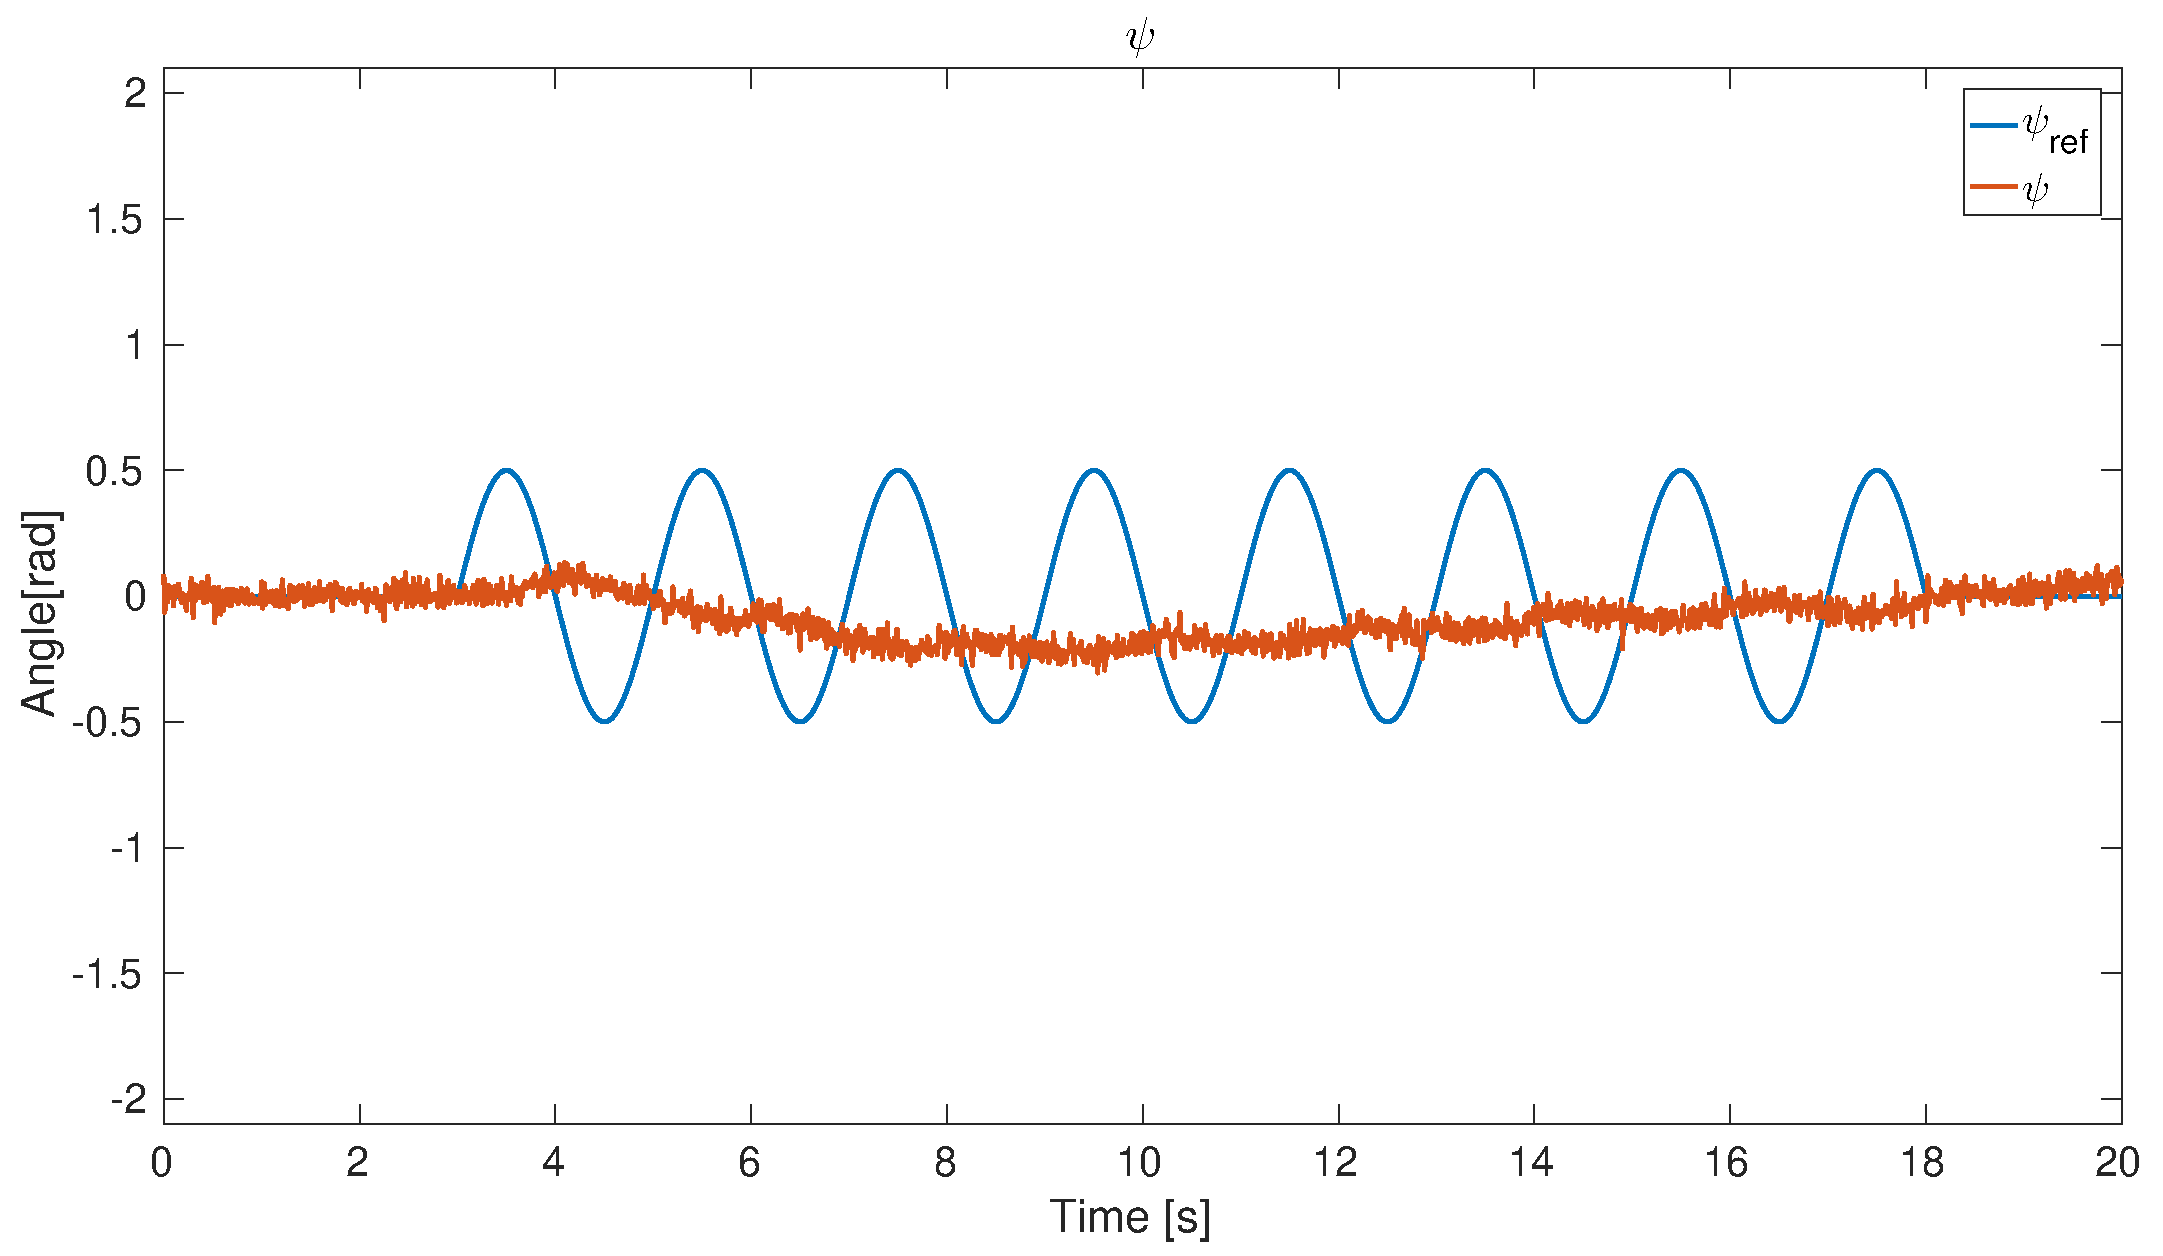
\includegraphics[width=0.4\textwidth]{simSinAllPsiA05}}
  \caption{\label{fig:AppSinAll05Attitude}%
    A sine signal with amplitude $0.5$ and frequency $0.5\ \hertz$ was applied in all attitude angles at the same time while using the attitude controller.}
\end{figure}

\begin{figure}
\centering
  \subfloat[][\label{fig:ApptestStepPhiTheta05RollAttitude} Test response in $\rollAngle$.]{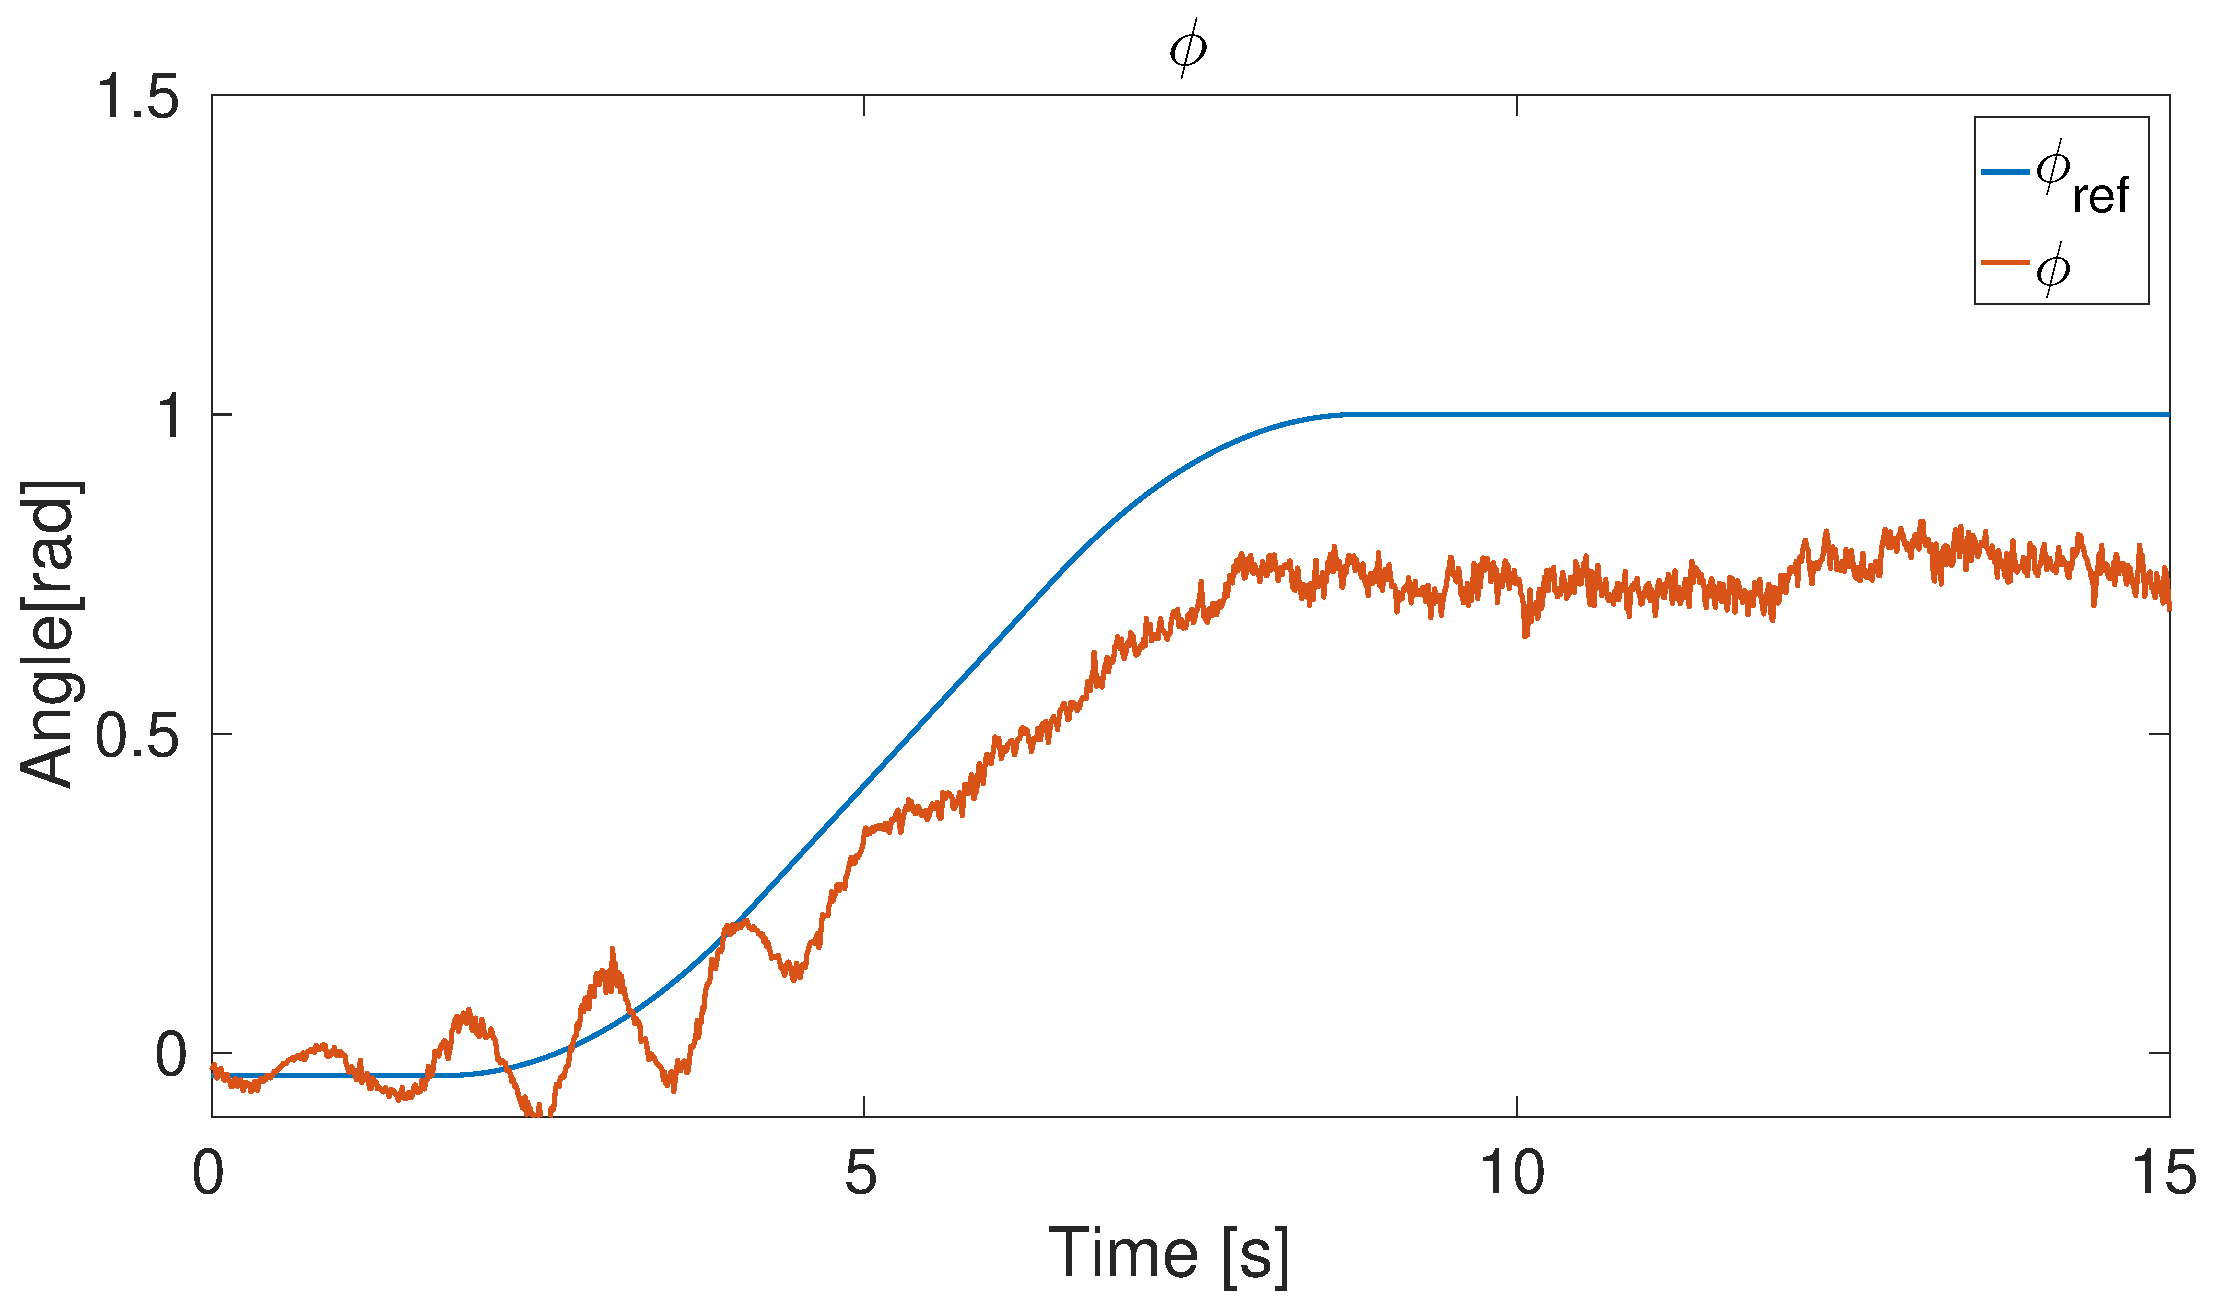
\includegraphics[width=0.4\textwidth]{testStepThetaPhiPhis3e10a1}}
  \qquad
  \subfloat[][\label{fig:AppsimStepPhiTheta05RollAttitude} Simulated response in $\rollAngle$.]{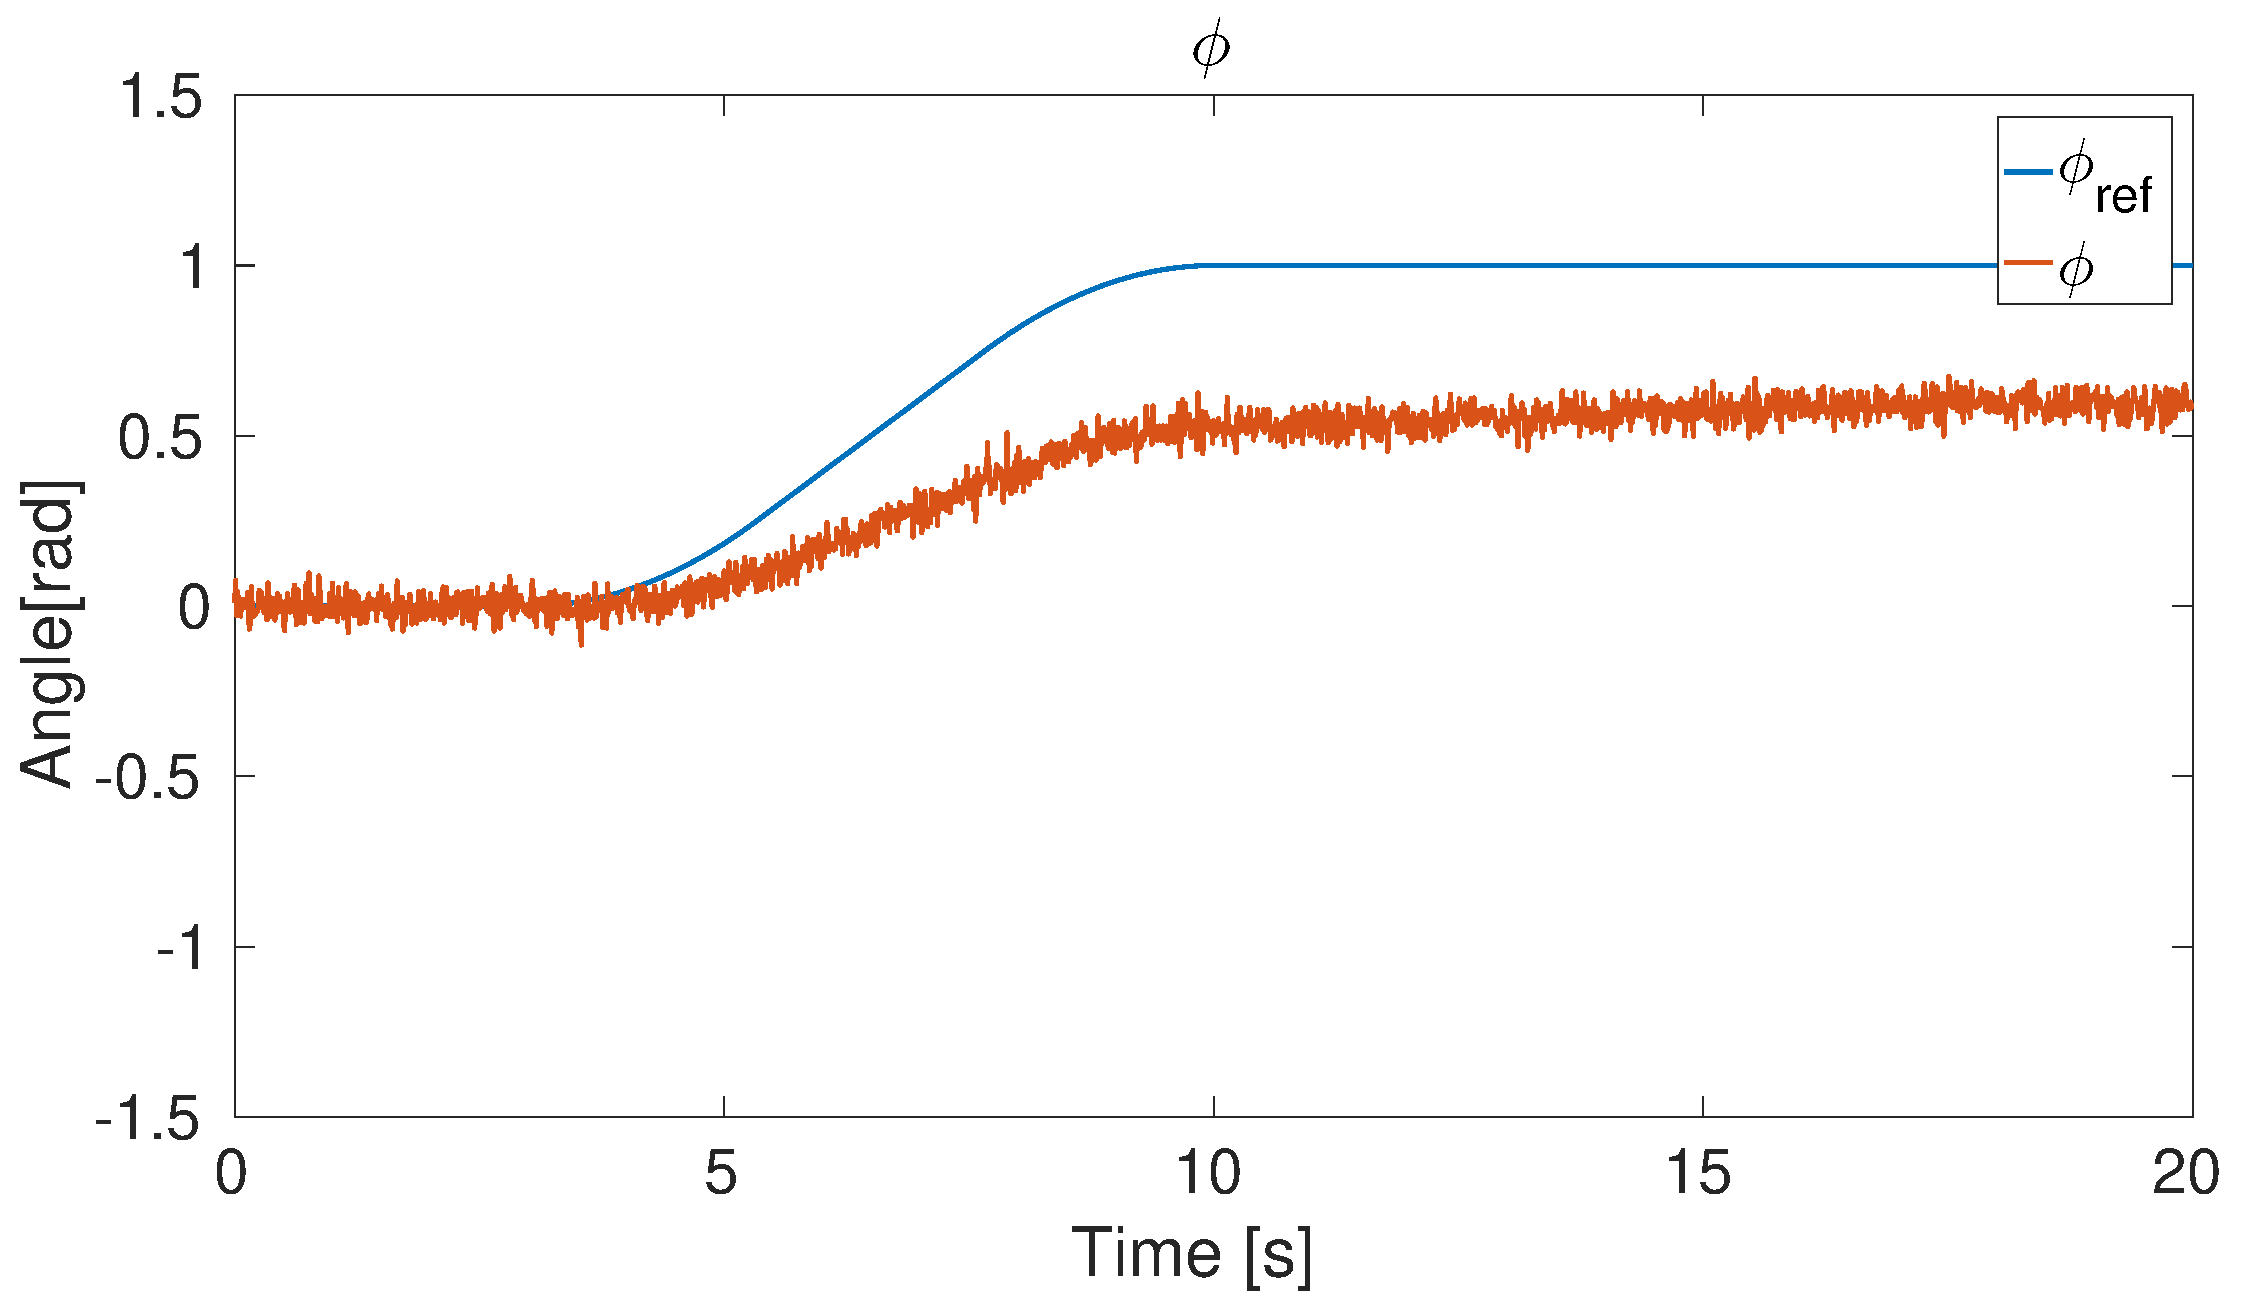
\includegraphics[width=0.4\textwidth]{simStepThetaPhiPhis3e10a1}}
  \qquad
  \subfloat[][\label{fig:ApptestStepPhiTheta05PitchAttitude}Test response in $\pitchAngle$.]{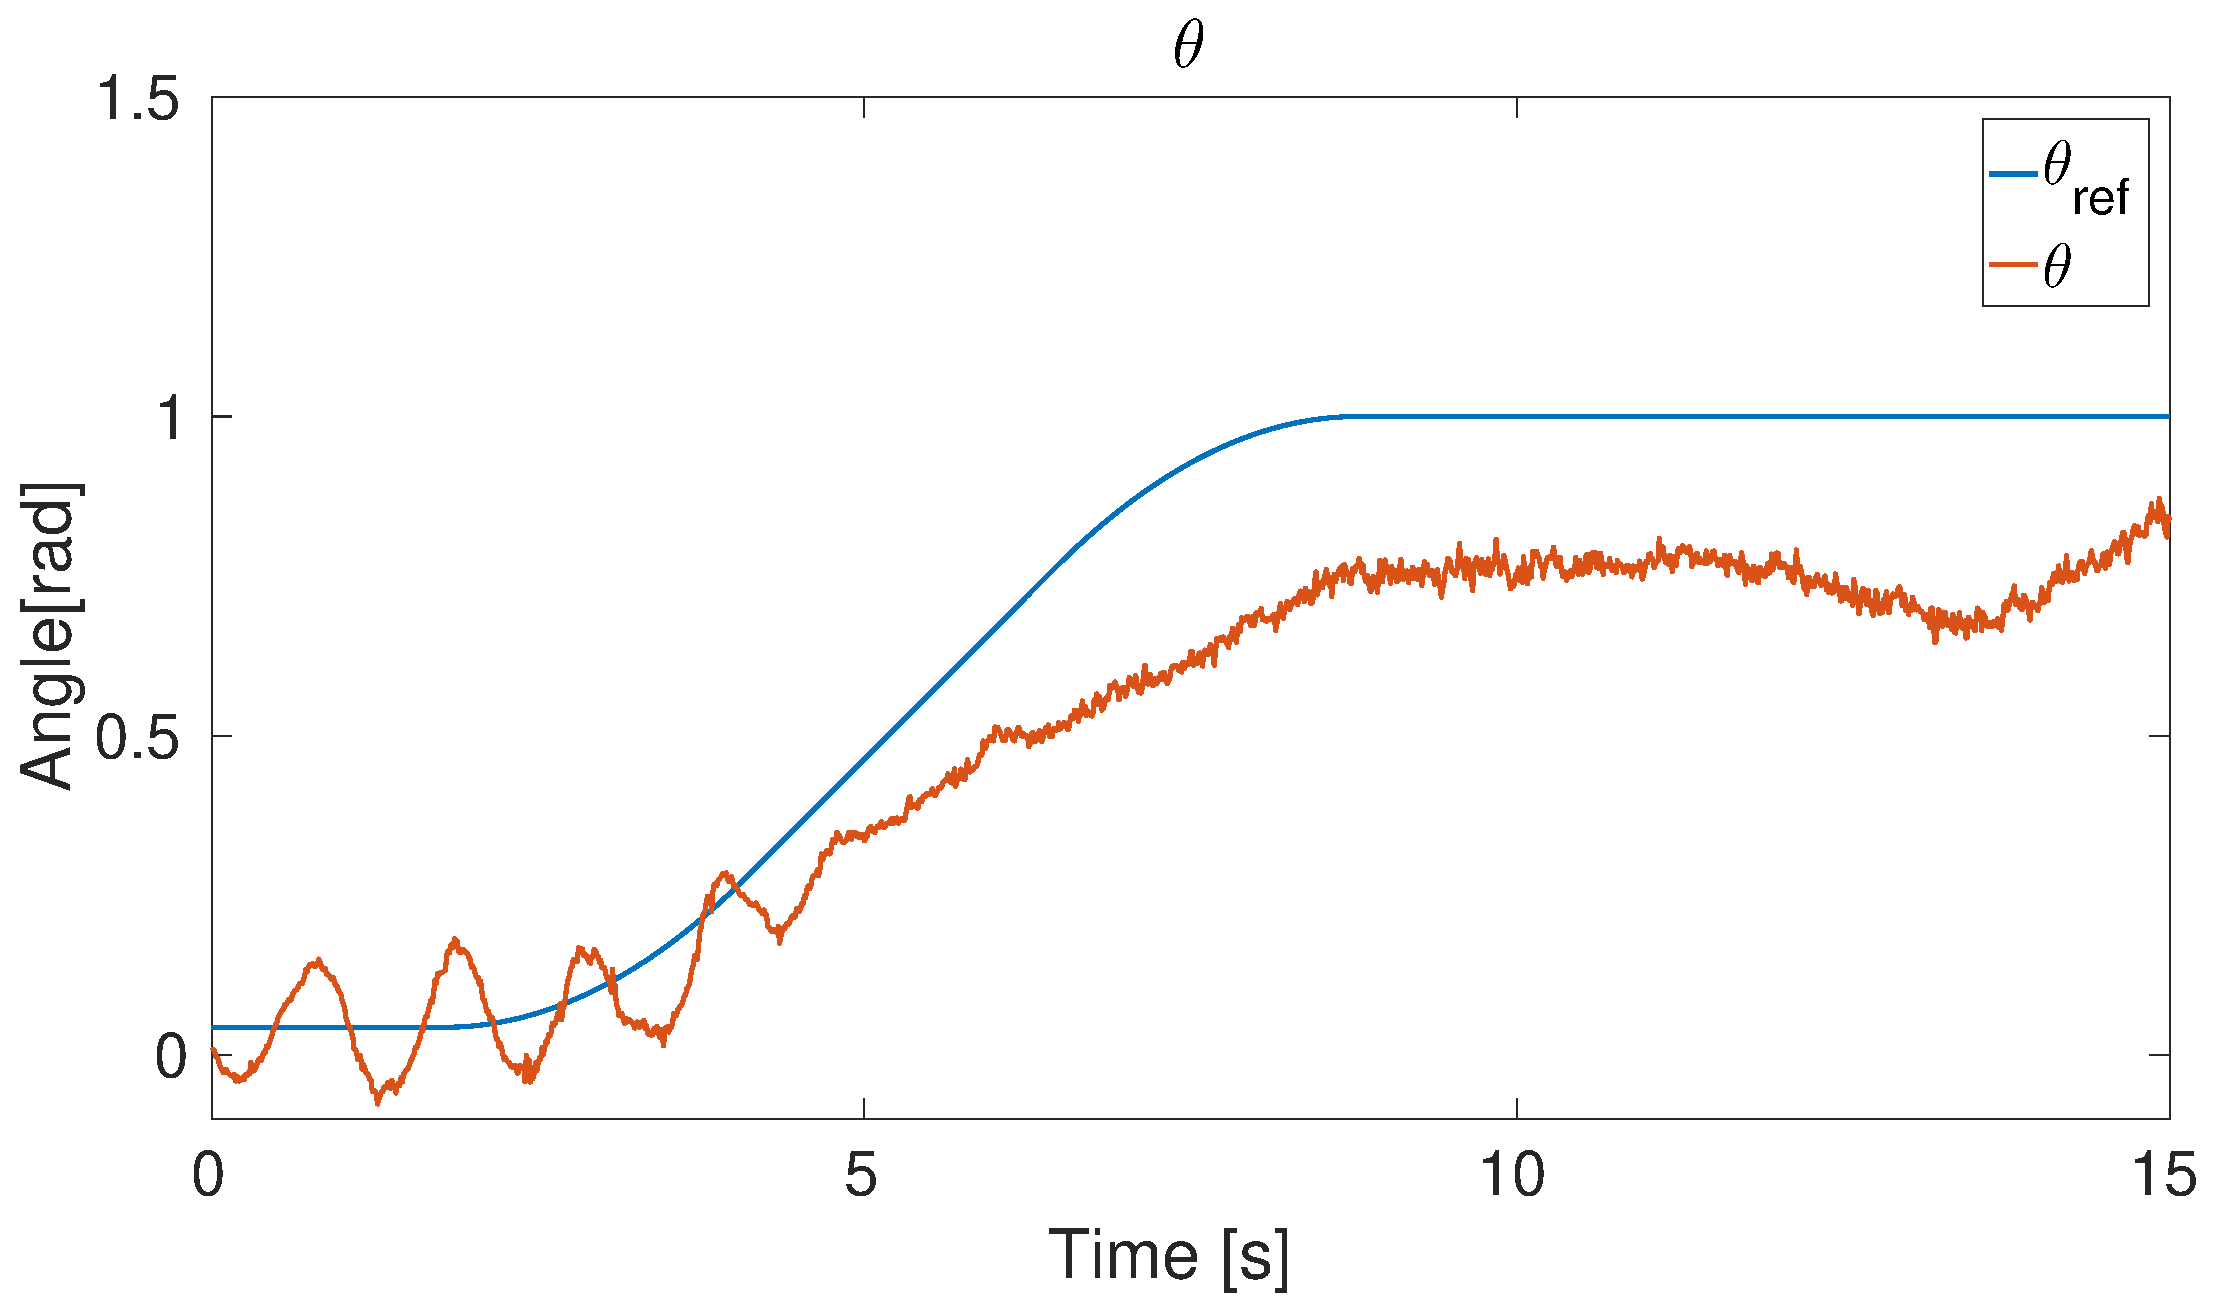
\includegraphics[width=0.4\textwidth]{testStepThetaPhiThetas3e10a1}}
  \qquad
  \subfloat[][\label{fig:AppsimStepPhiTheta05PitchAttitude} Simulated response in $\pitchAngle$.]{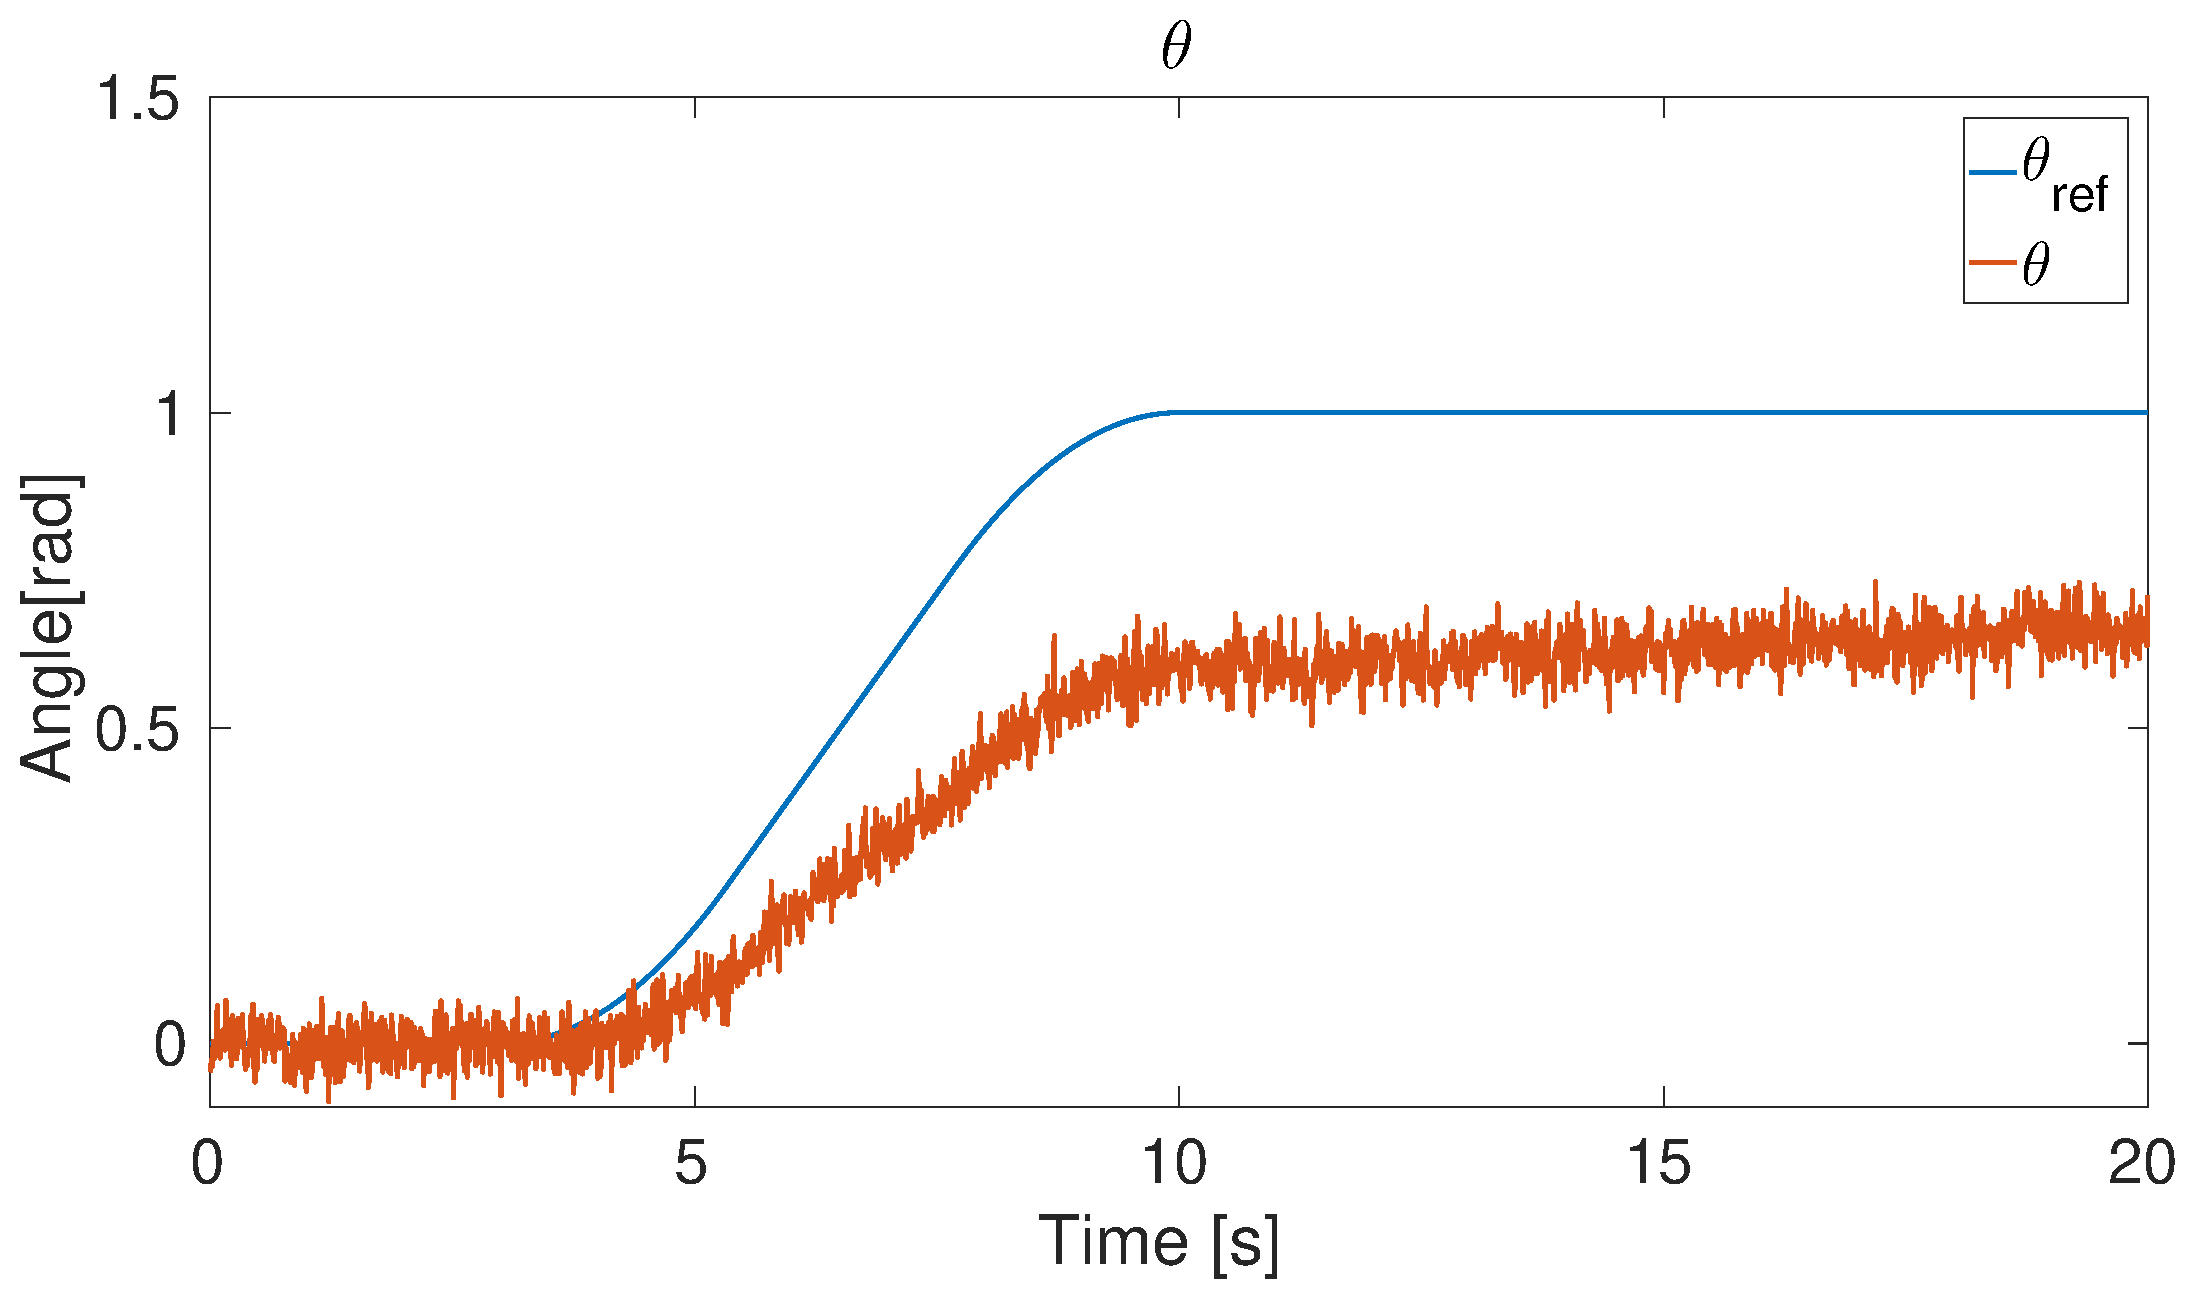
\includegraphics[width=0.4\textwidth]{simStepThetaPhiThetas3e10a1}}
  \caption{\label{fig:AppStepPhiThetaAttitude}%
  Smooth steps with $q_{\text{0}} = 0$, $q_{\text{f}} = 1$, $t_{\text{s}} = 3$, $t_{\text{f}} = 15$ and $V = 1.5 (q_{\text{f}} - q_{\text{0}})/(t_{\text{f}} - t_{\text{s}}))$ were applied in \pitchAngle and \rollAngle at the same time while using the attitude controller. The attitude angle $\yawAngle$ was kept free during the test.}
\end{figure}

%%%%%%%%%%%%%%%%%%%%%%%%%%%Rate%%%%%%%%%%%%%%%%
\begin{figure}[tbp]
  \centering
  \subfloat[][\label{fig:ApptestStepP} Test response in $\rollVelocity$.]{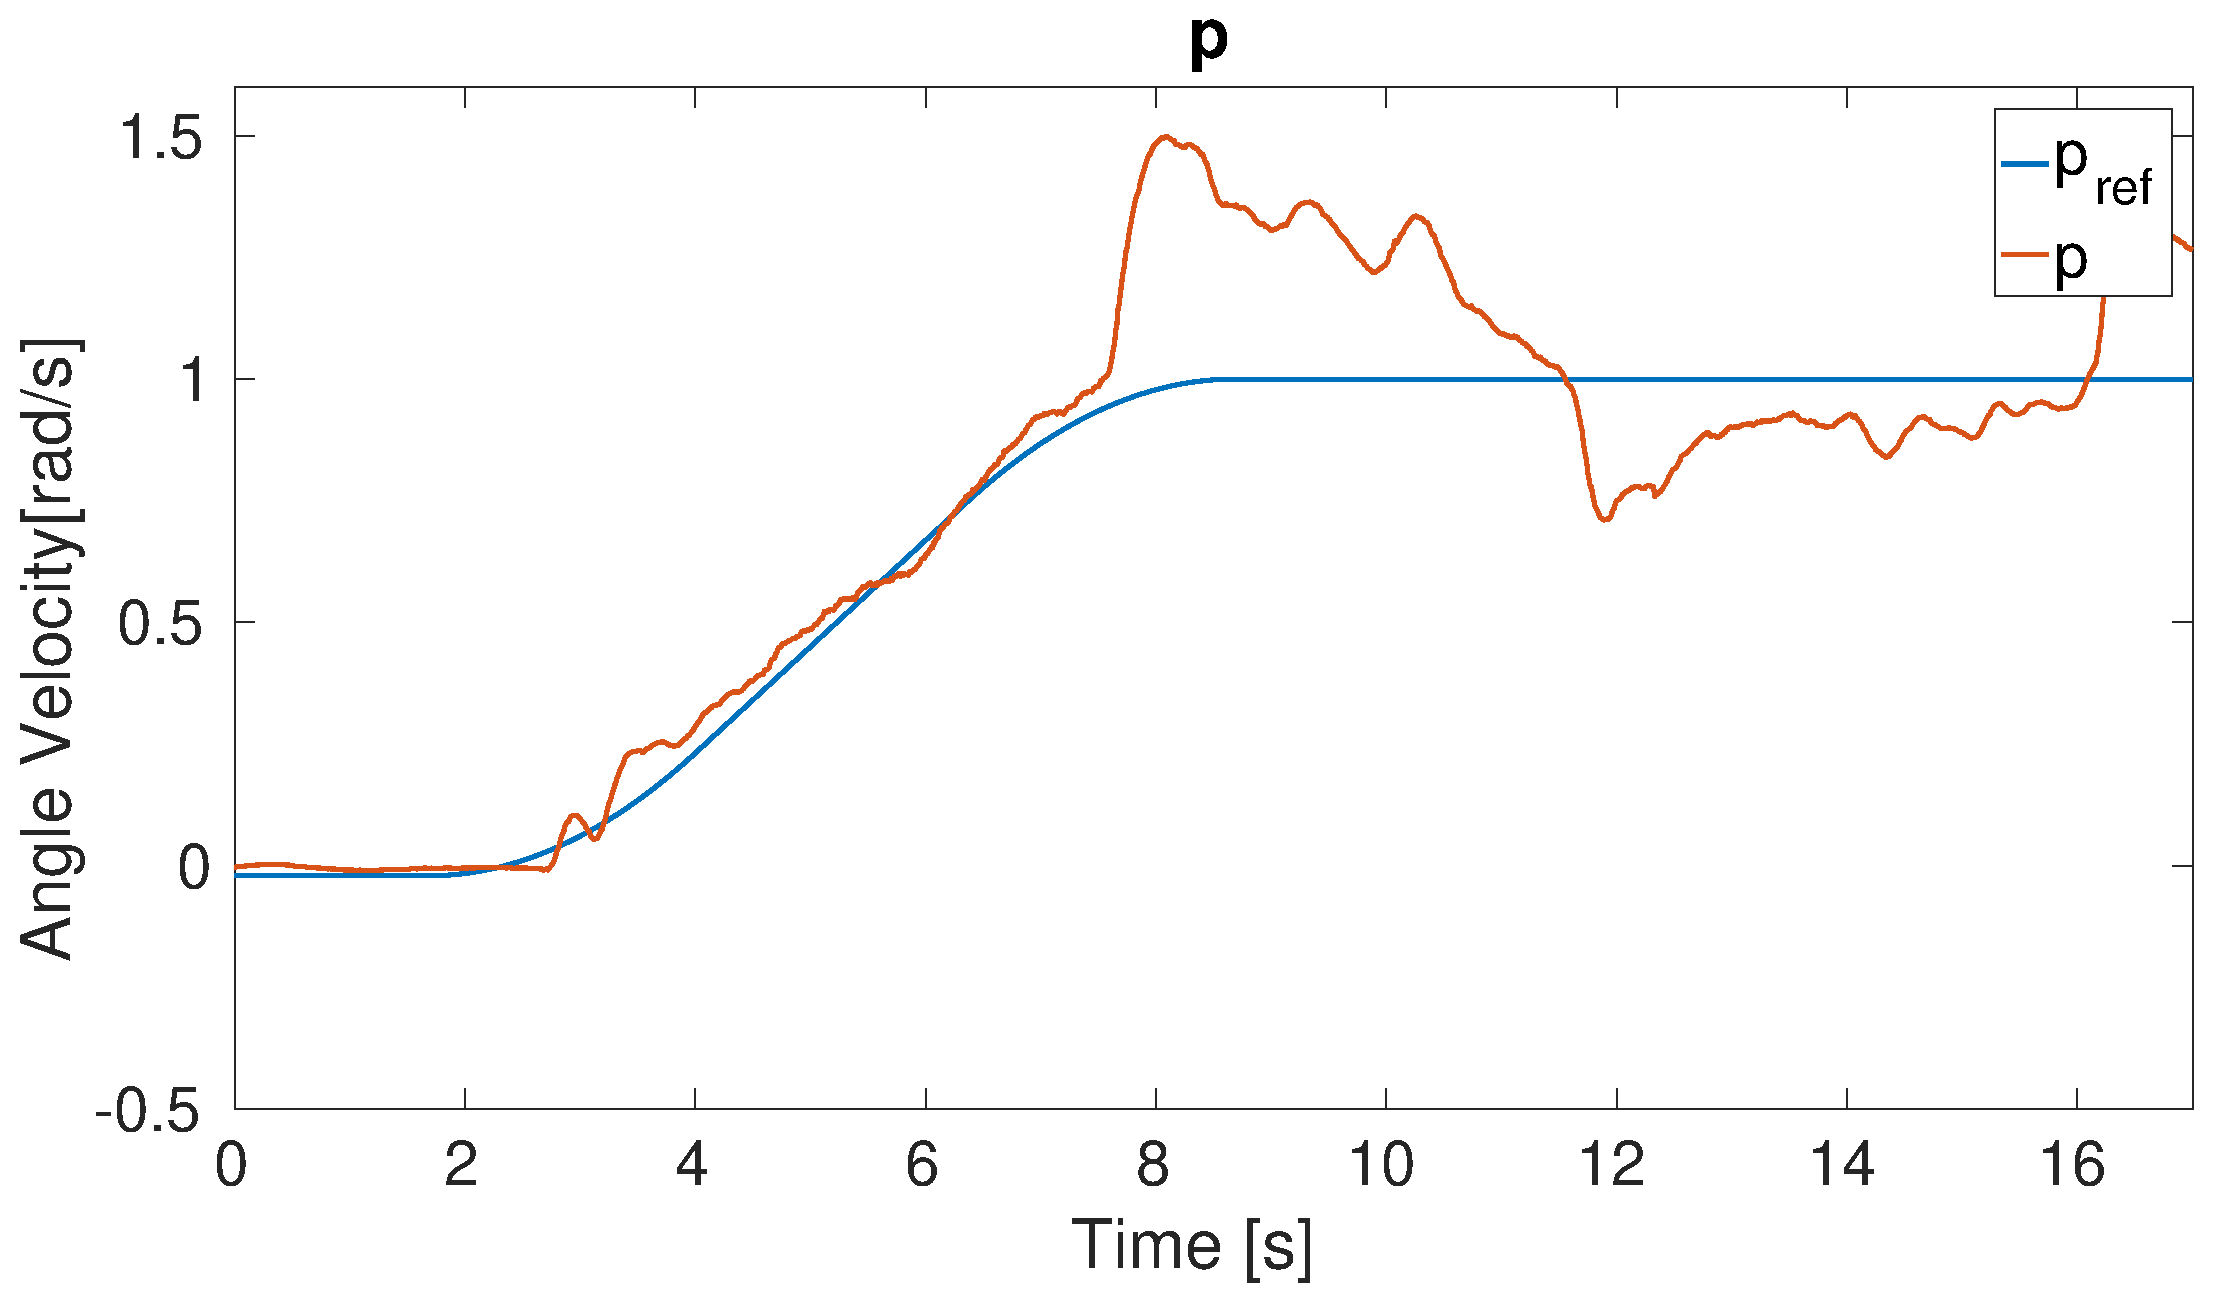
\includegraphics[width=0.4\textwidth]{testStepPs3e10a1}}
  \qquad
  \subfloat[][\label{fig:AppsimStepP} Simulated response in $\rollVelocity$.]{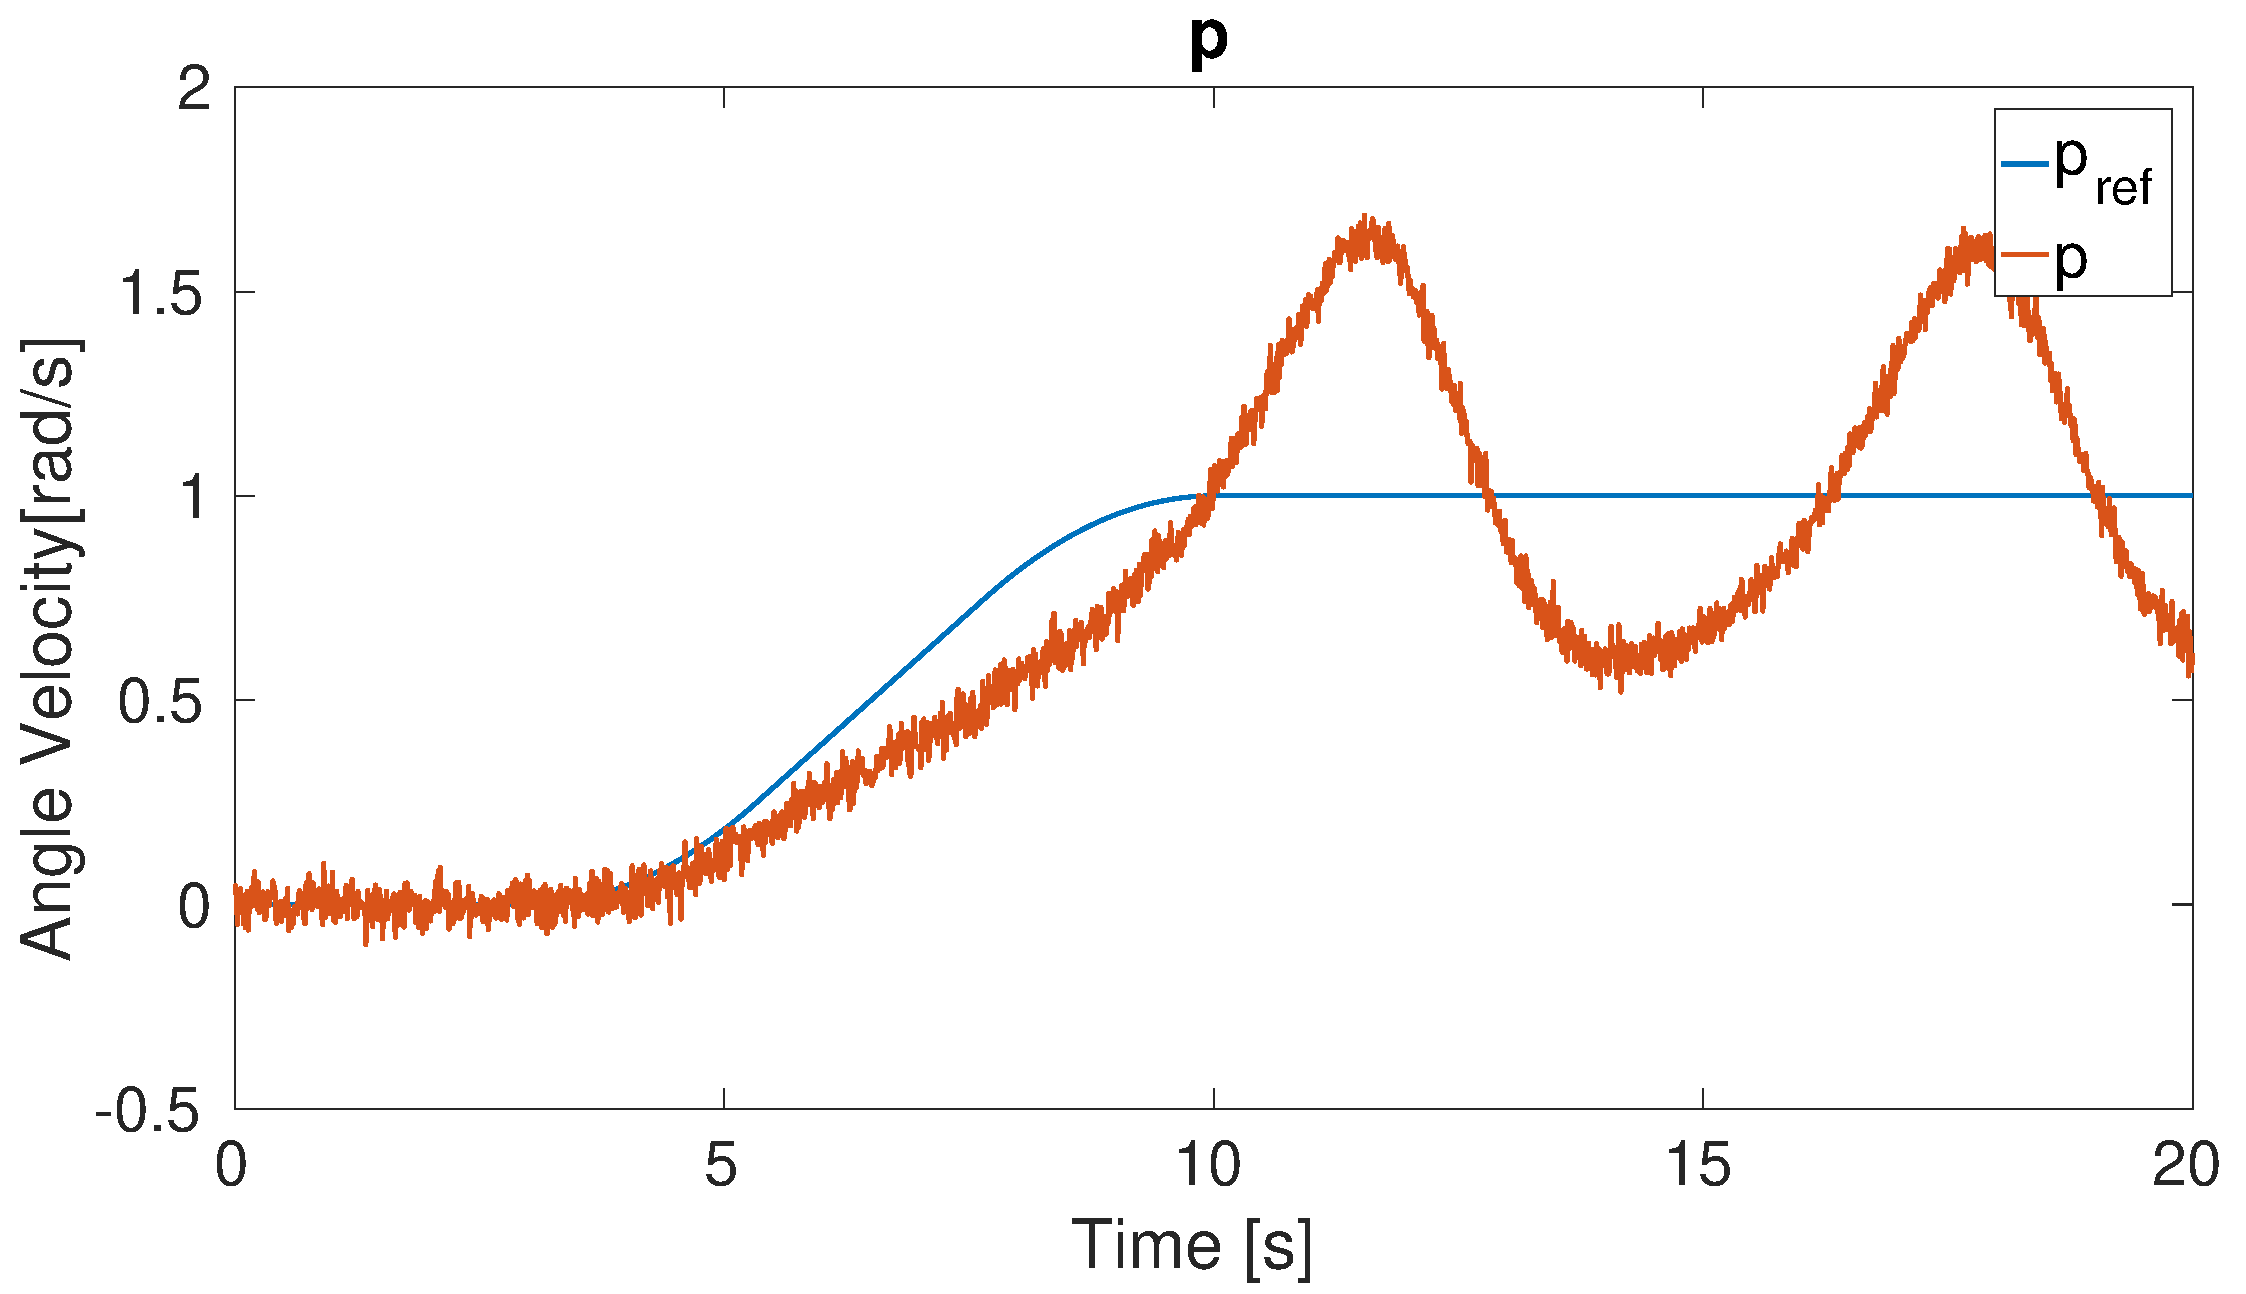
\includegraphics[width=0.4\textwidth]{simStepPs3e10a1}}
  \qquad
  \subfloat[][\label{fig:ApptestStepQ} Test response in $\pitchVelocity$.]{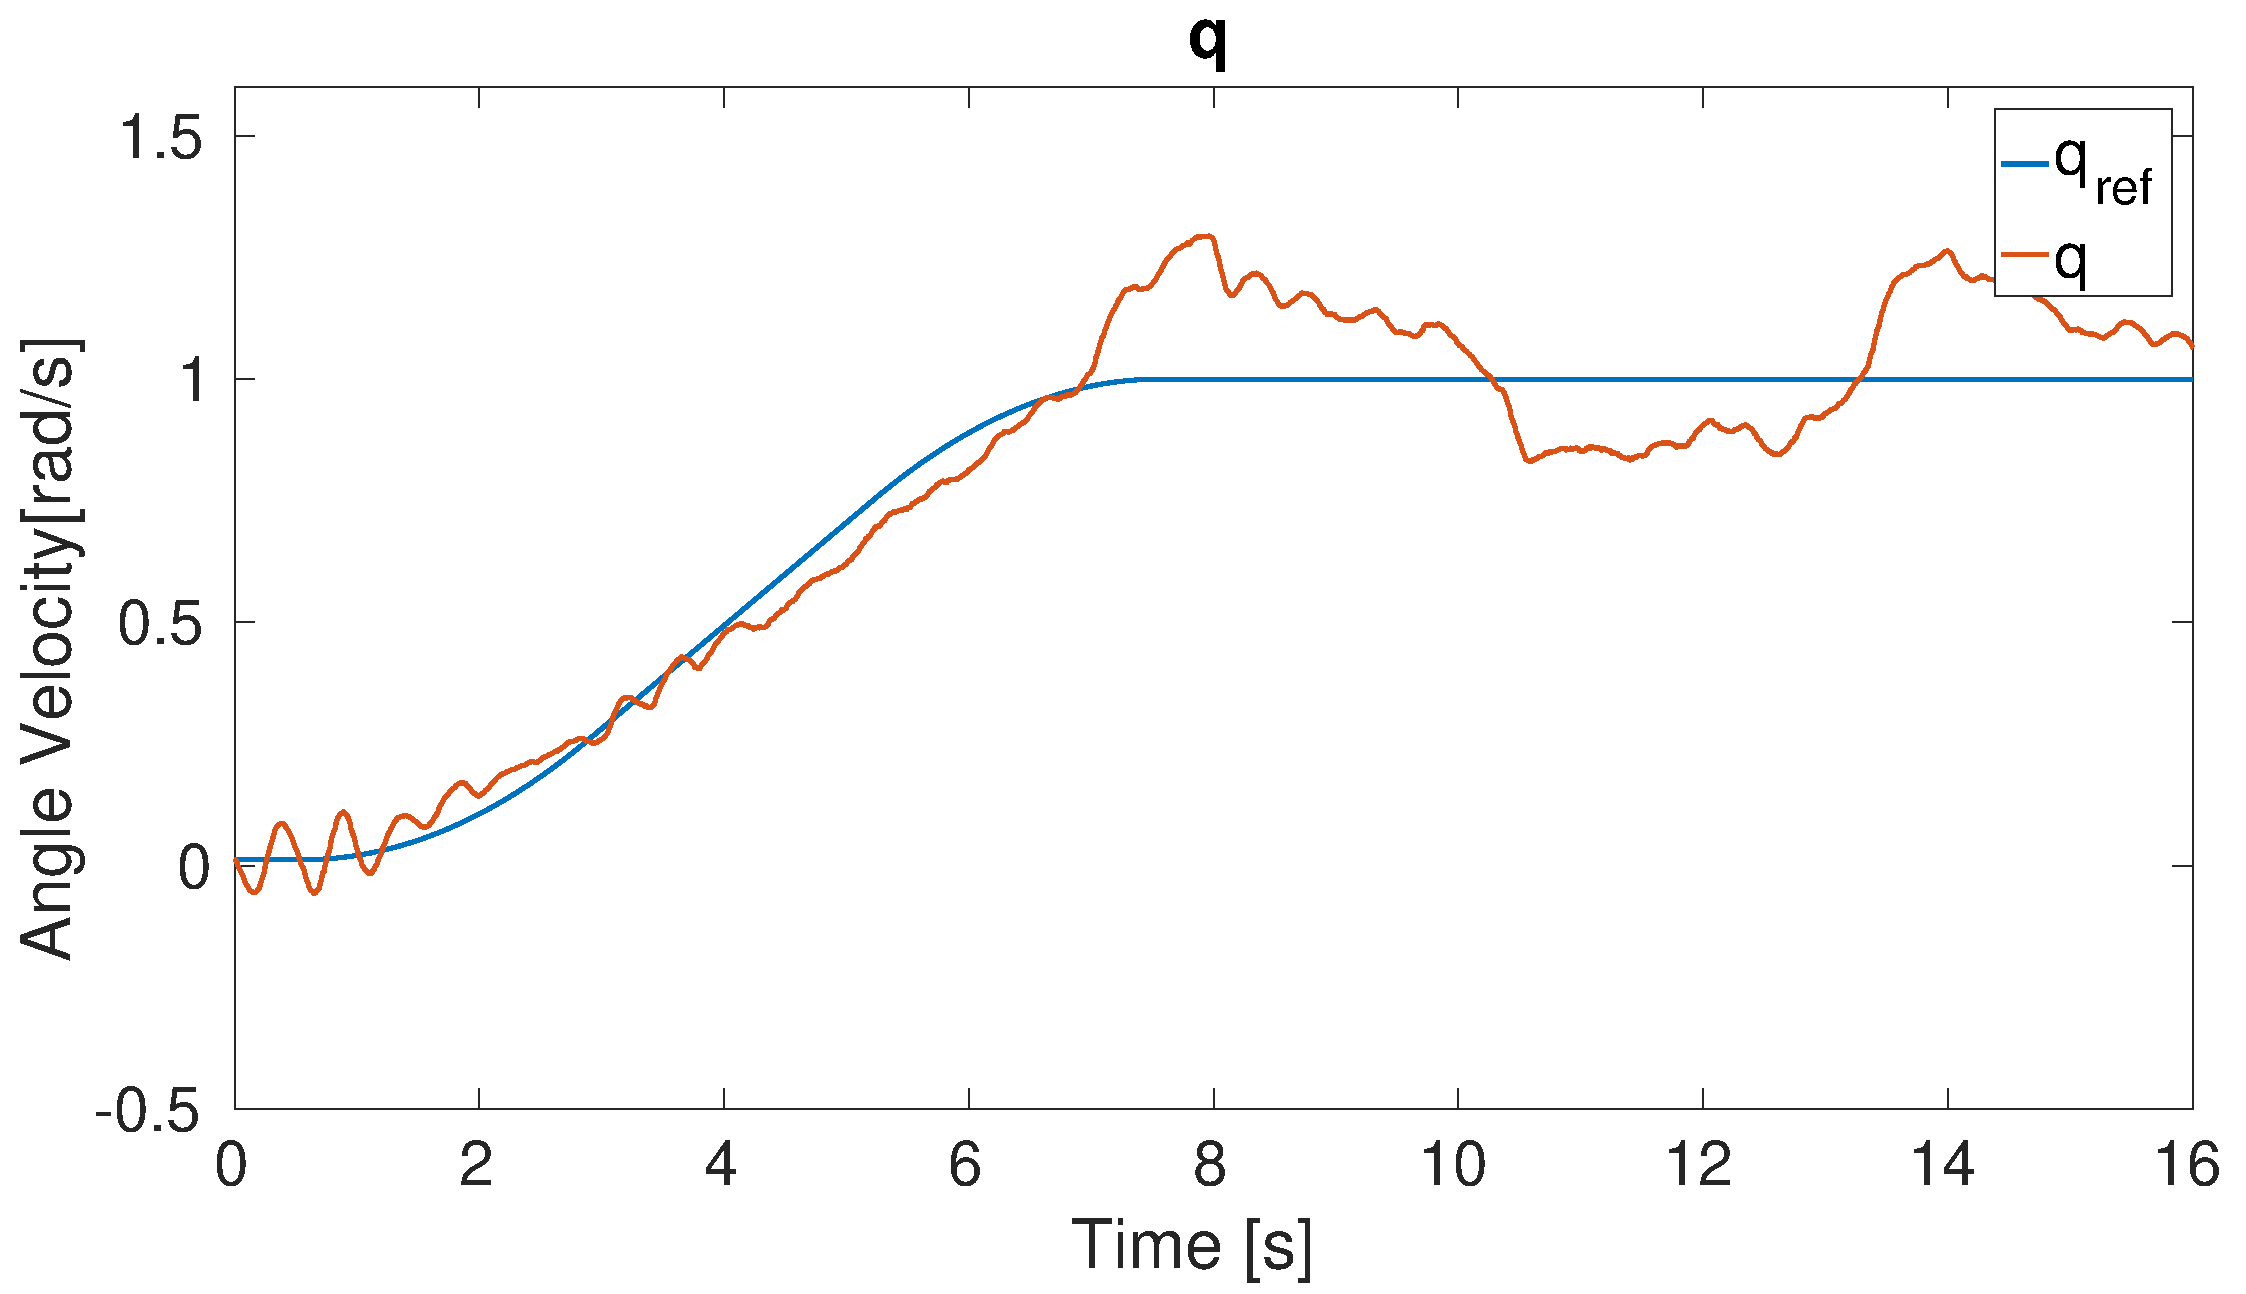
\includegraphics[width=0.4\textwidth]{testStepQs3e10a1}}
  \qquad
  \subfloat[][\label{fig:AppsimStepQ} Simulated response in $\pitchVelocity$.]{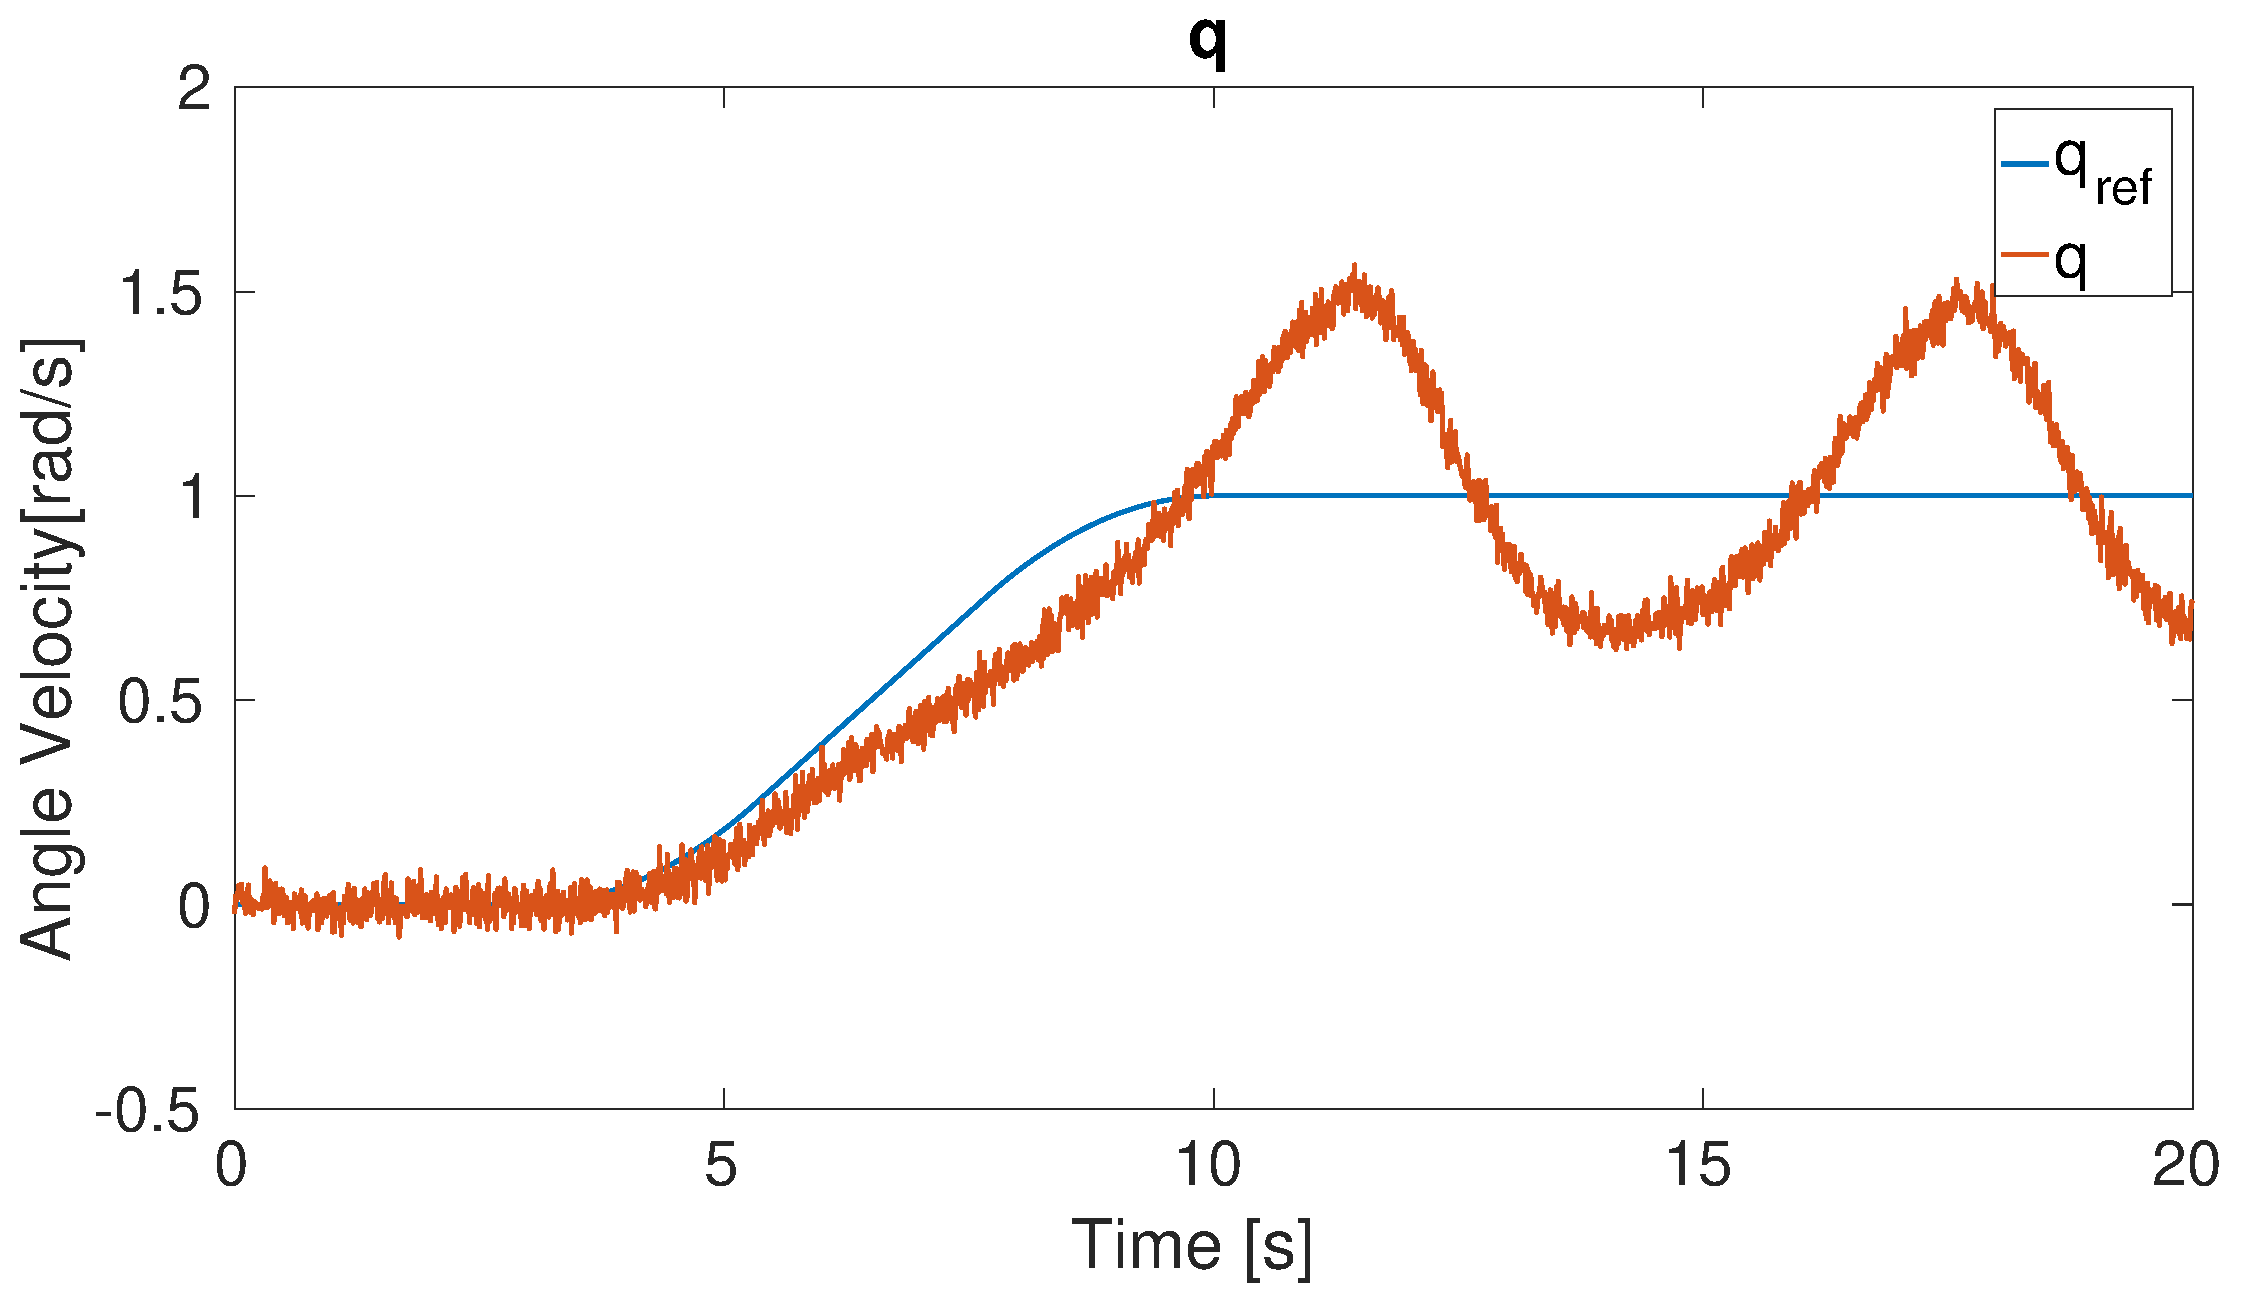
\includegraphics[width=0.4\textwidth]{simStepQs3e10a1}}
  \qquad
  \subfloat[][\label{fig:ApptestStepR} Test response in $\yawVelocity$.]{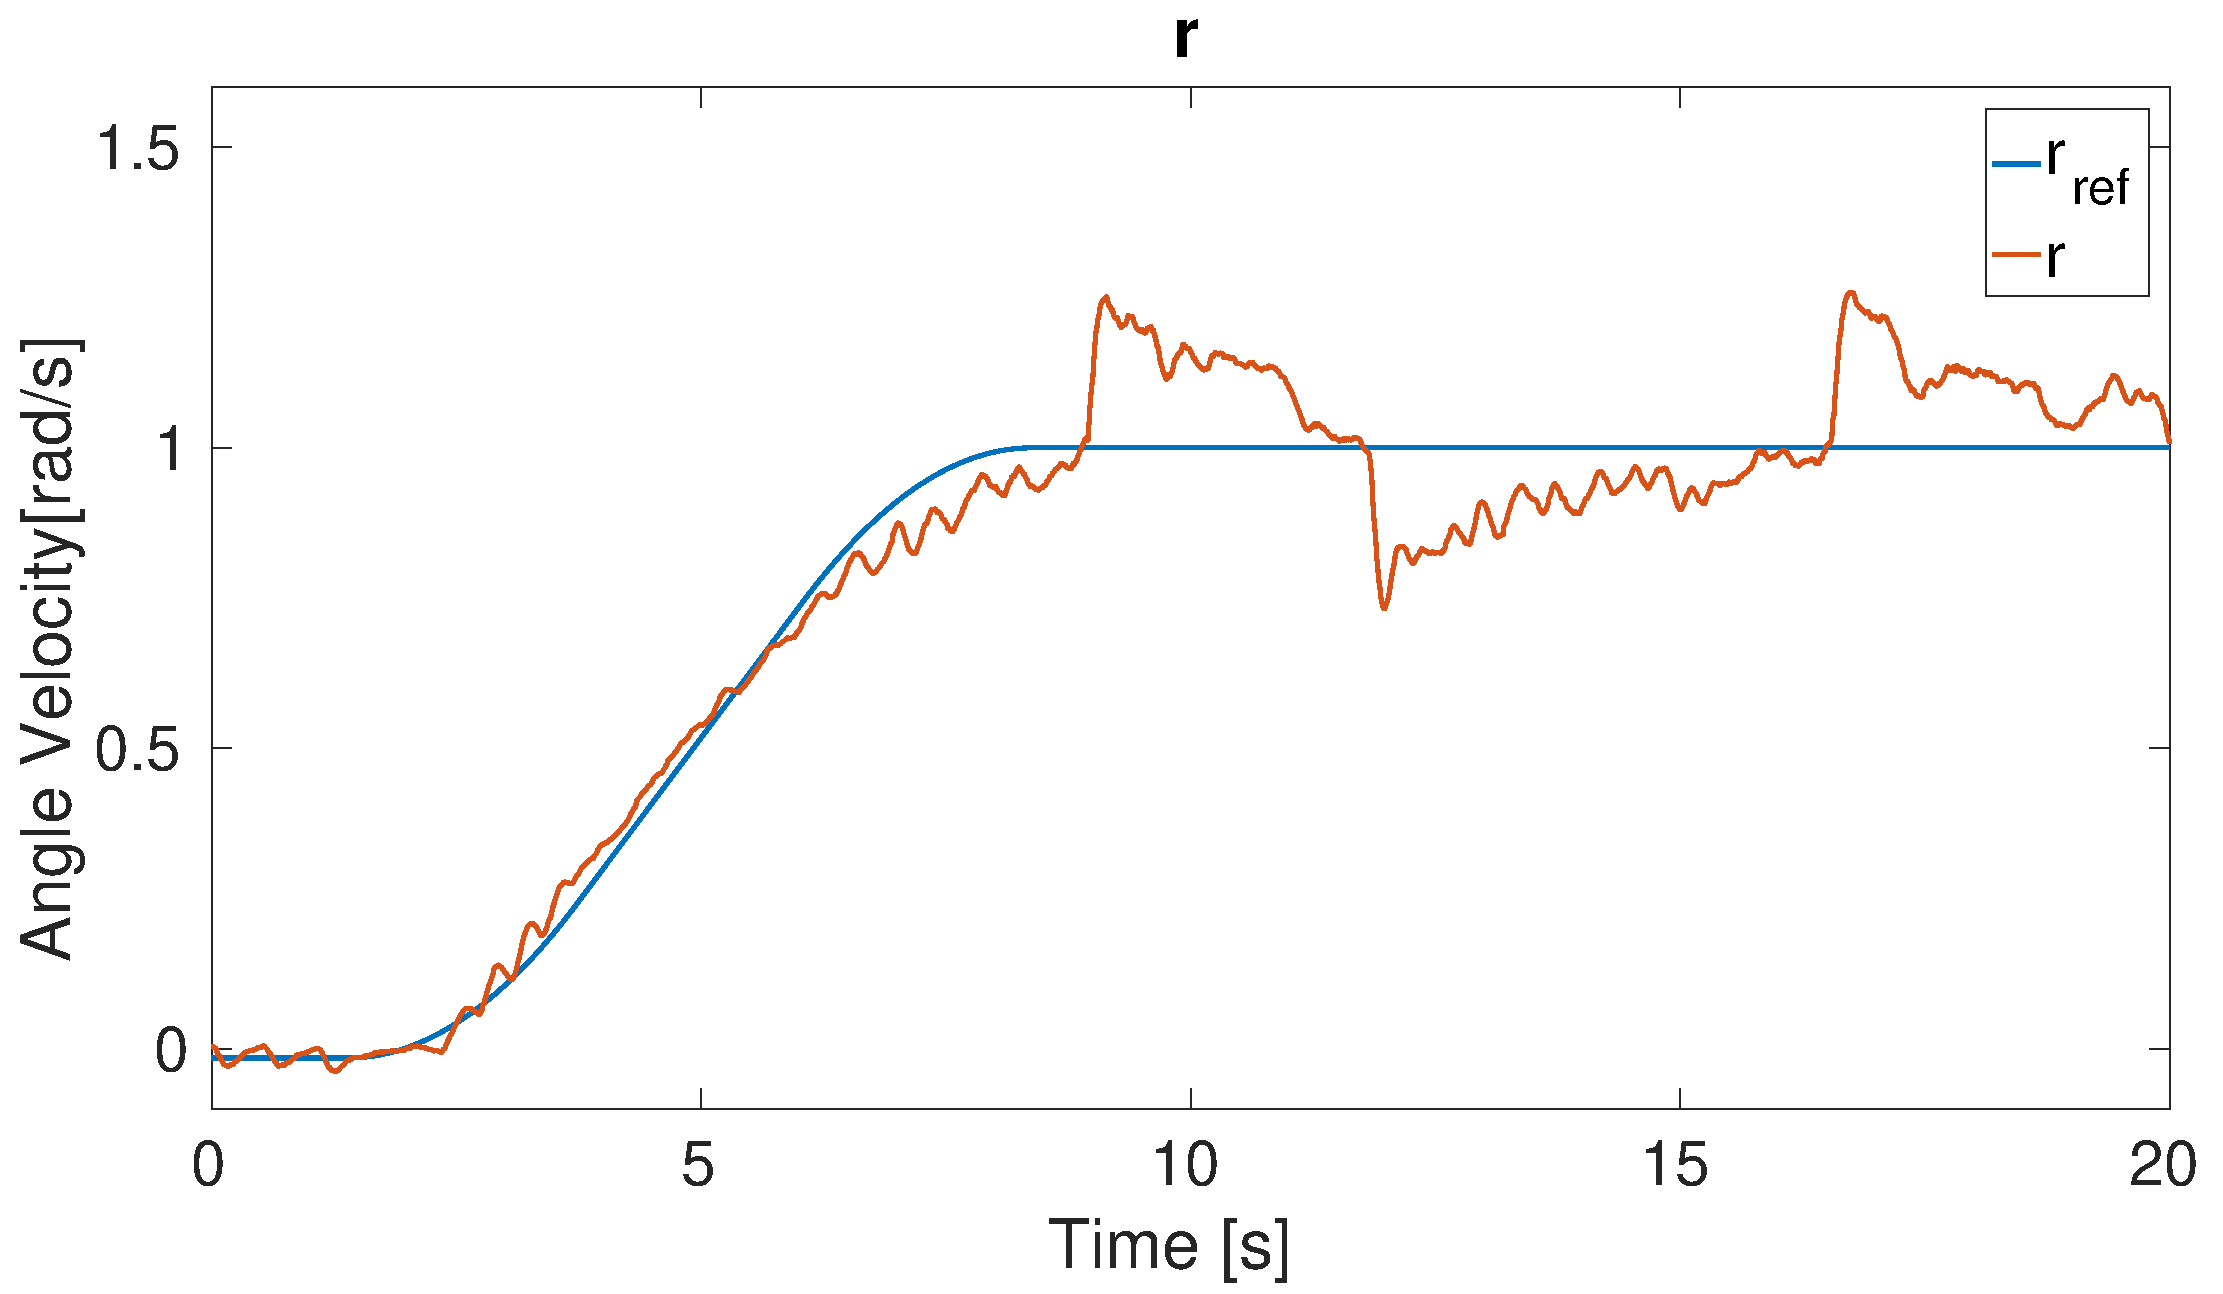
\includegraphics[width=0.4\textwidth]{testStepRs3e10a1}}
  \qquad
  \subfloat[][\label{fig:AppsimStepR} Simulated response in $\yawVelocity$.]{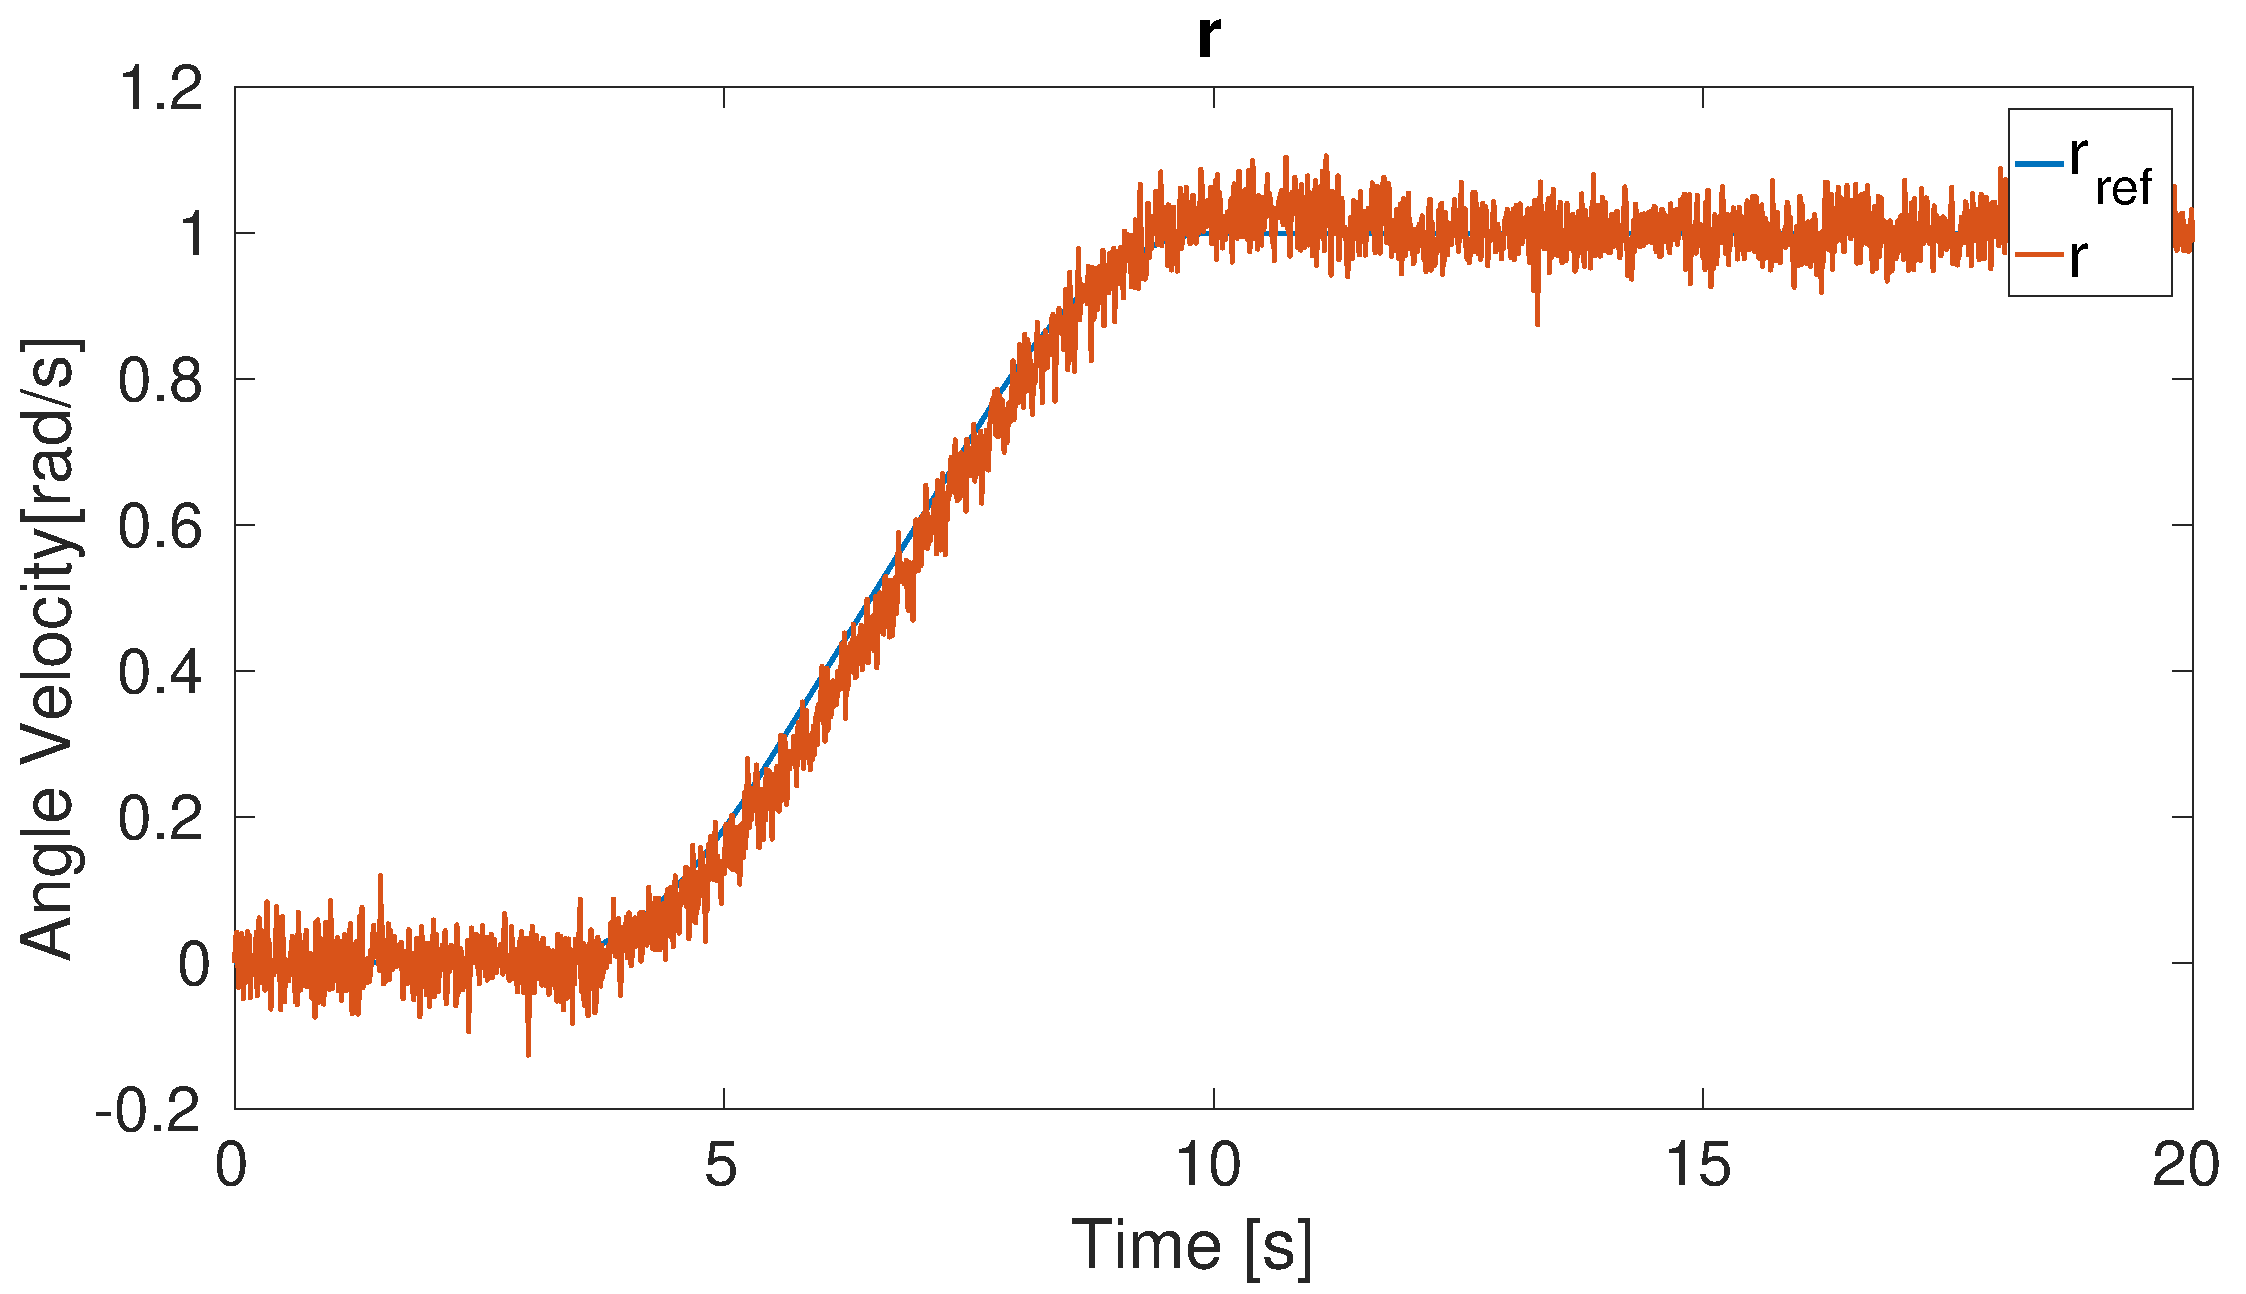
\includegraphics[width=0.4\textwidth]{simStepRs3e10a1}}
   \caption{\label{fig:AppStepRate}%
   A smooth step with $q_{\text{0}} = 0$, $q_{\text{f}} = 1$, $t_{\text{s}} = 3$, $t_{\text{f}} = 15$ and $V = 1.5 (q_{\text{f}} - q_{\text{0}})/(t_{\text{f}} - t_{\text{s}}))$ was applied in one angular velocity at a time while using the rate controller. While a smooth step was applied in one angular velocity the other angular velocities were controlled with the reference zero.}
\end{figure}

\begin{figure}
\centering
  \subfloat[][\label{fig:ApptestStepAllPRate} Test response in $\rollVelocity$.]{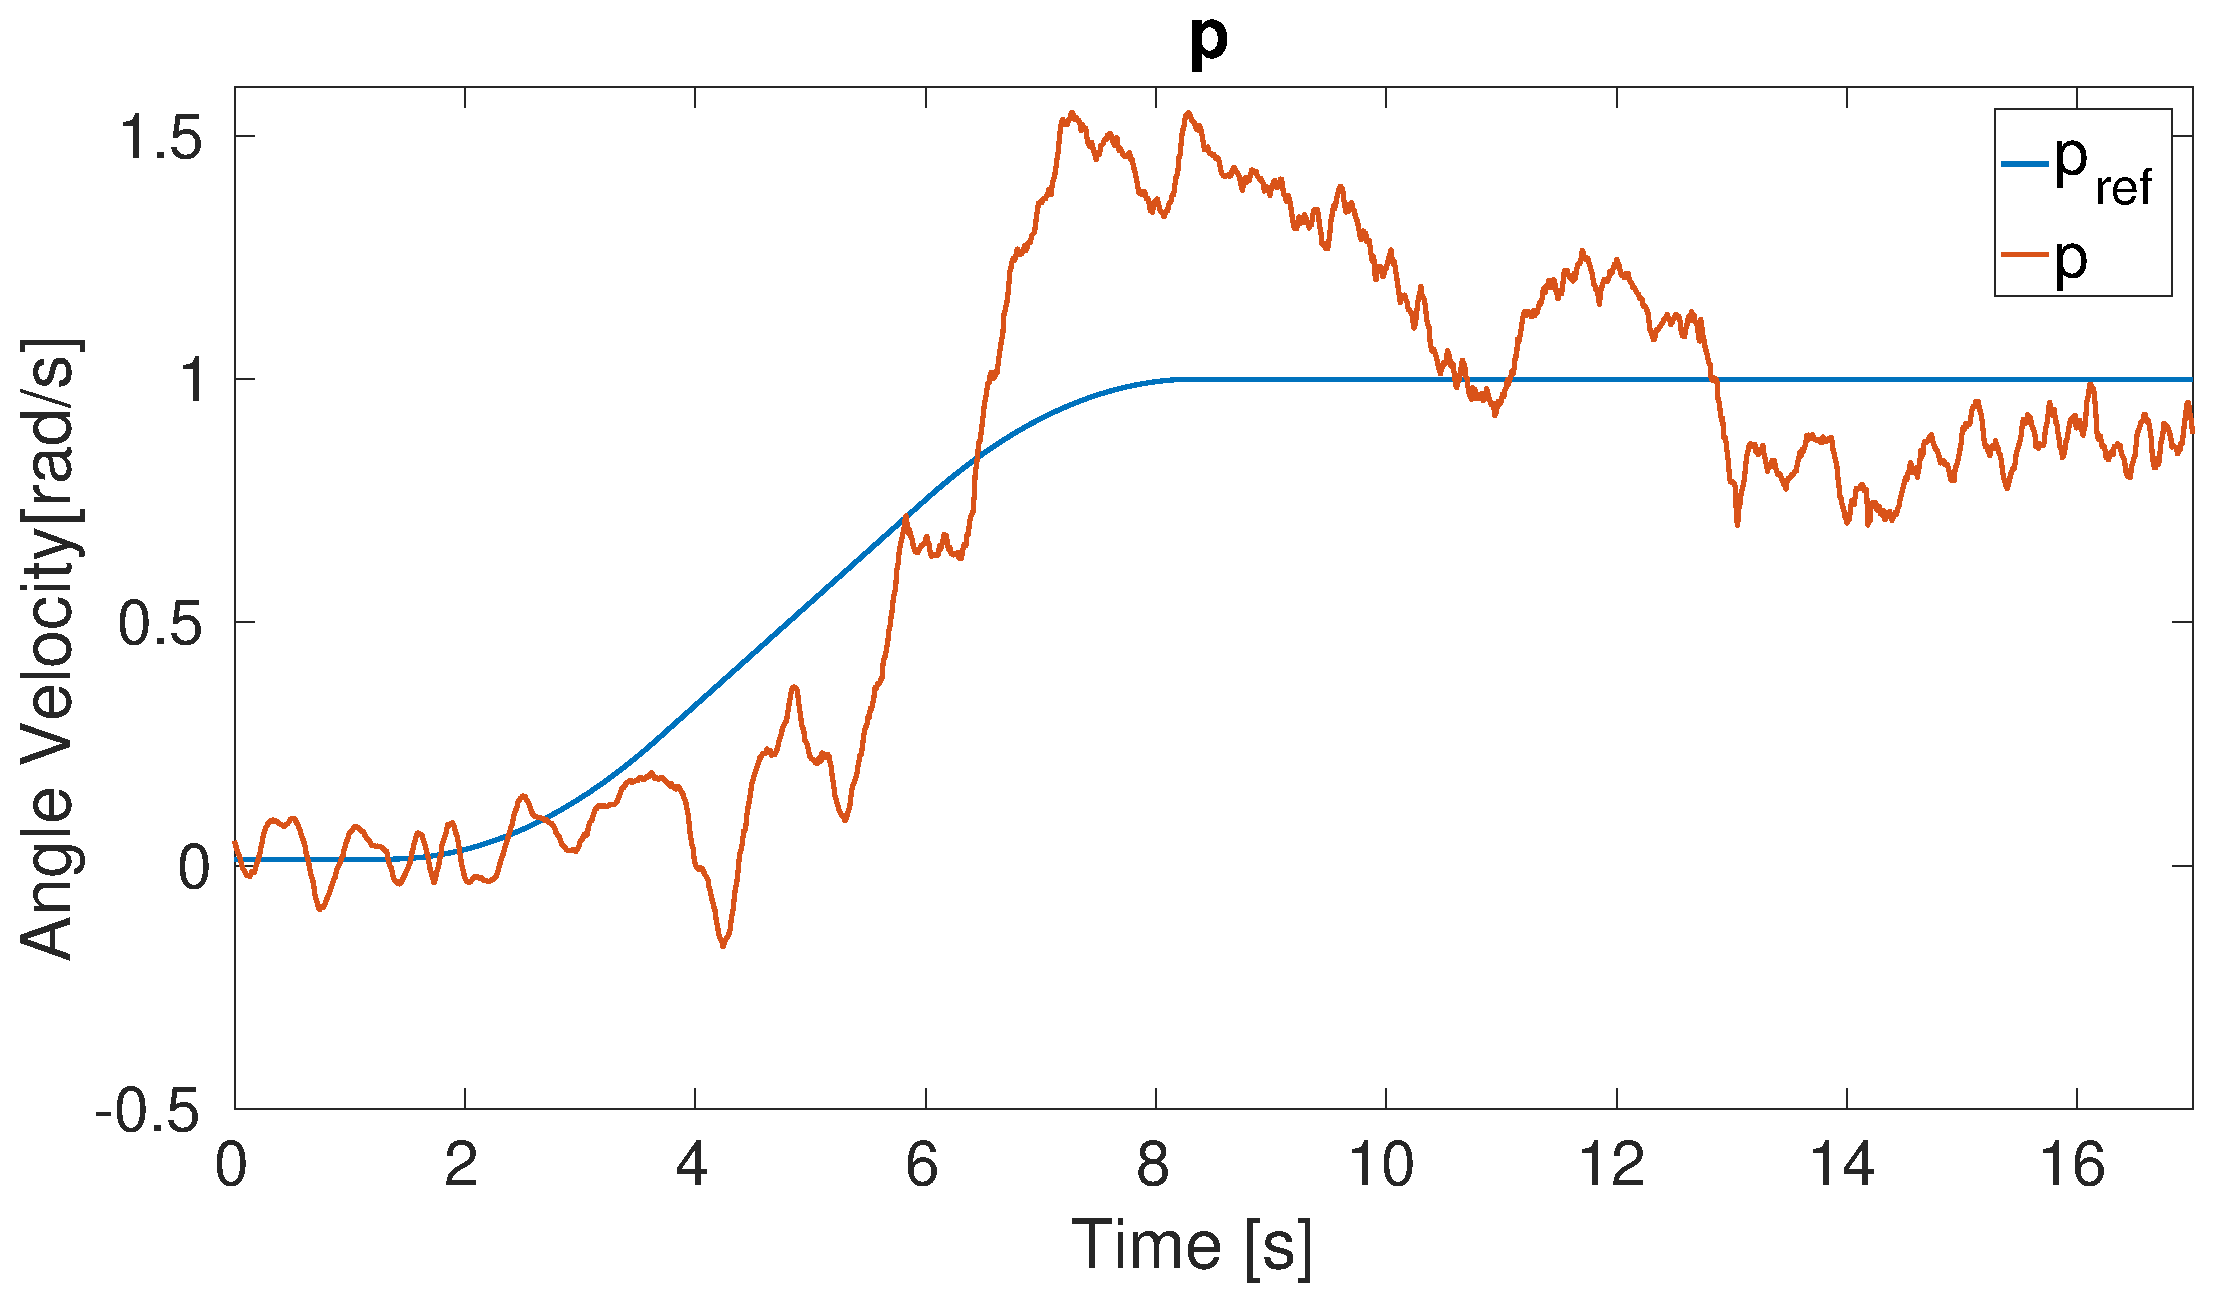
\includegraphics[width=0.4\textwidth]{testStepAllPs3e10a1}}
  \qquad 
  \subfloat[][\label{fig:AppsimStepAllPRate} Simulated response in $\rollVelocity$.]{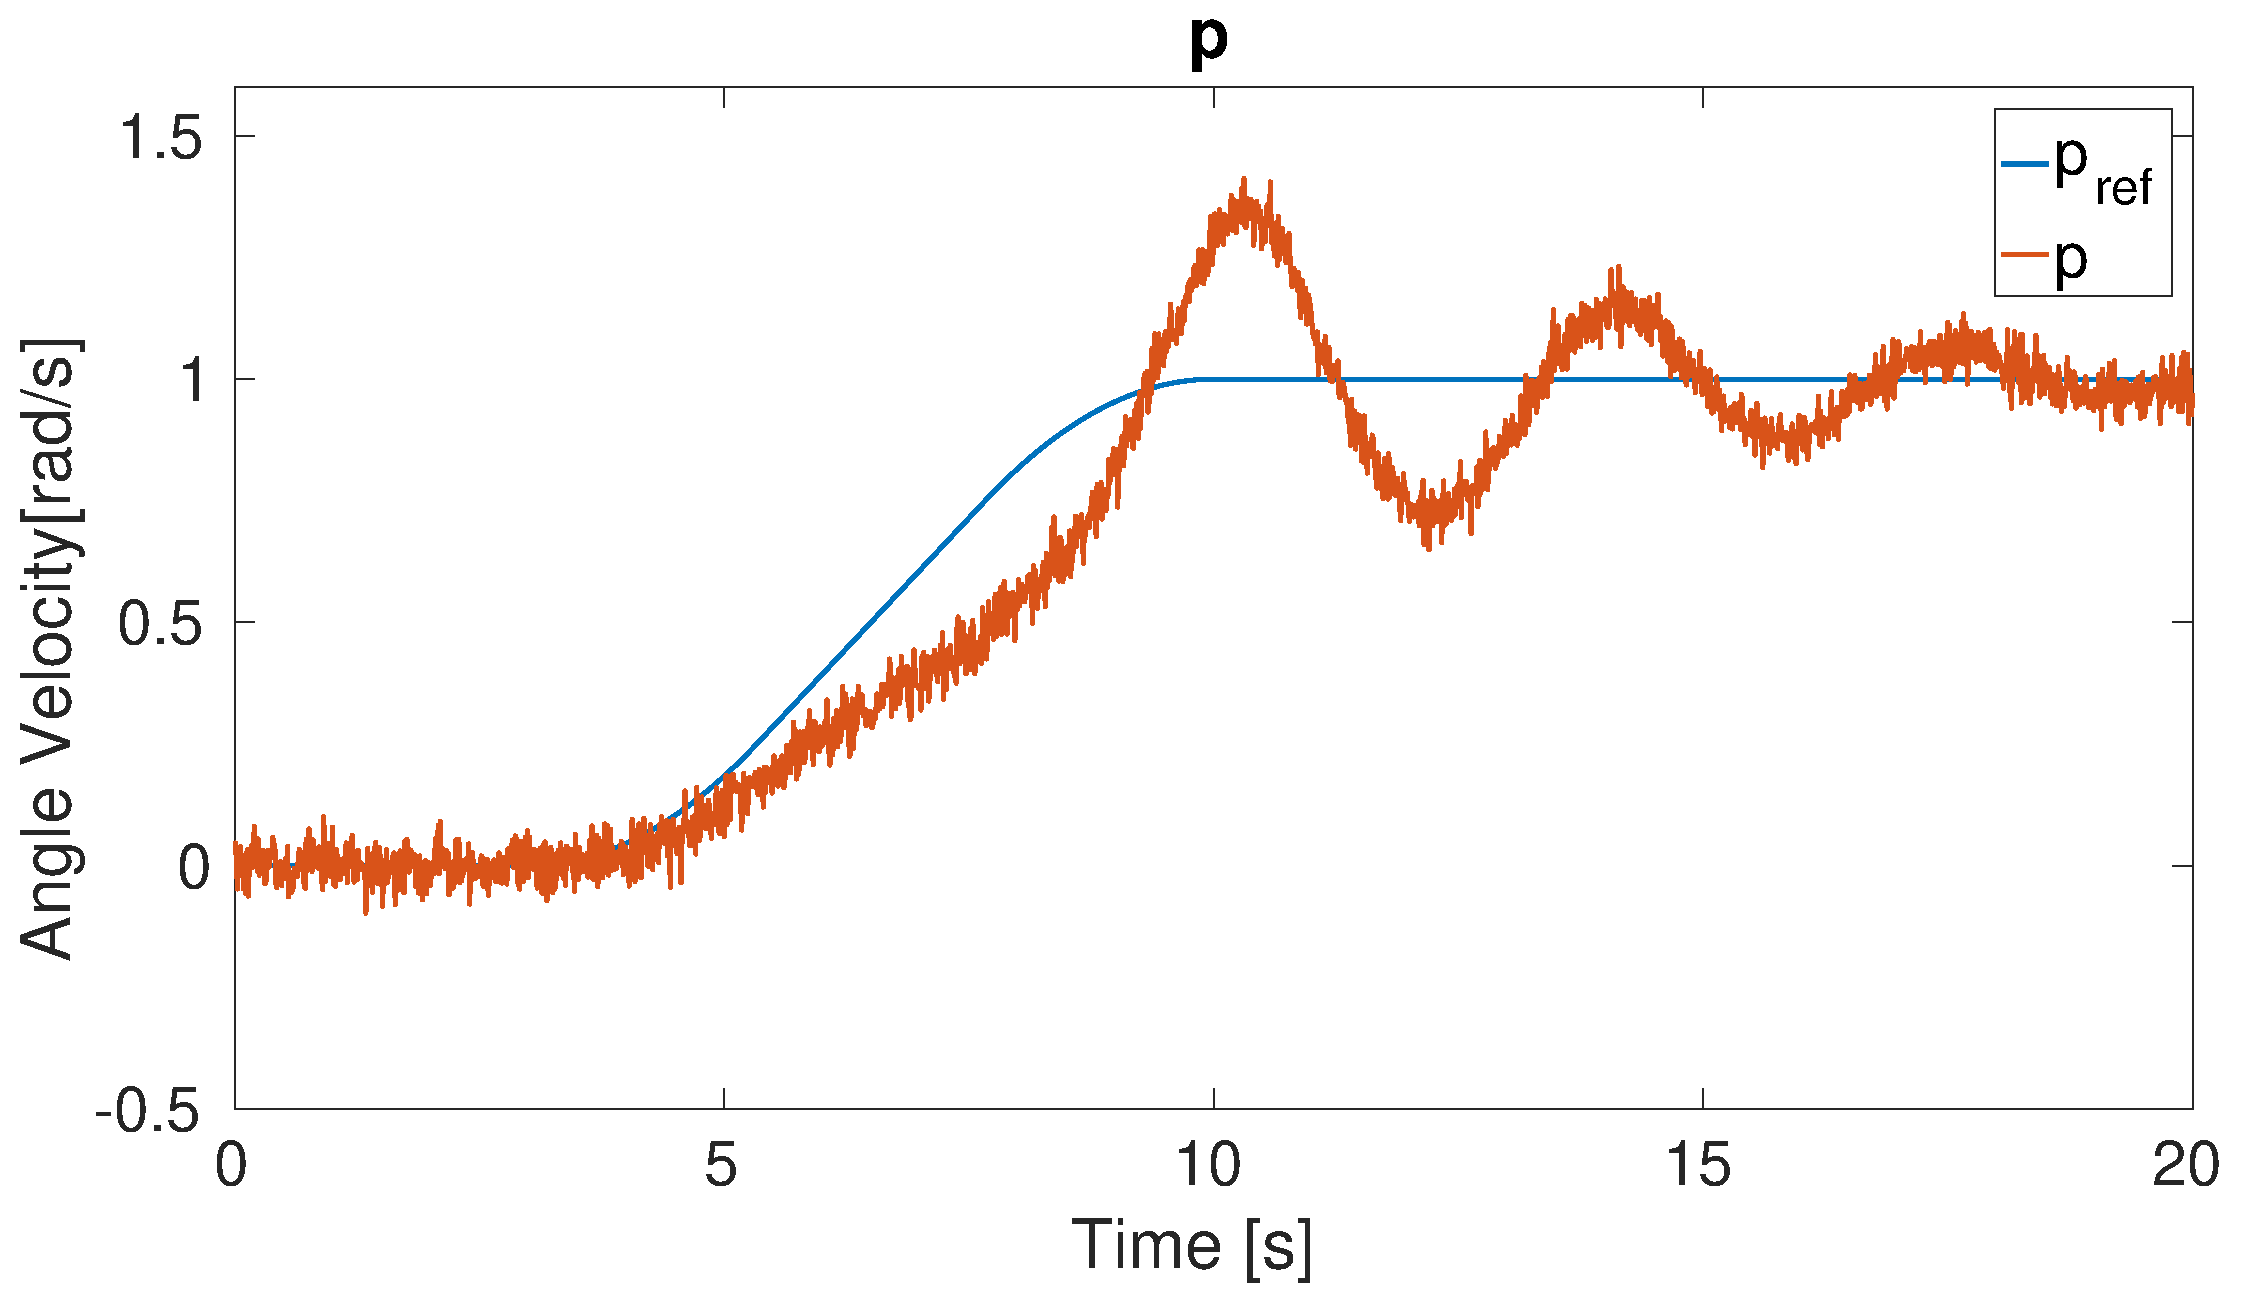
\includegraphics[width=0.4\textwidth]{simStepAllPs3e10a1}}
  \qquad
  \subfloat[][\label{fig:ApptestStepAllQRate} Test response in $\pitchVelocity$.]{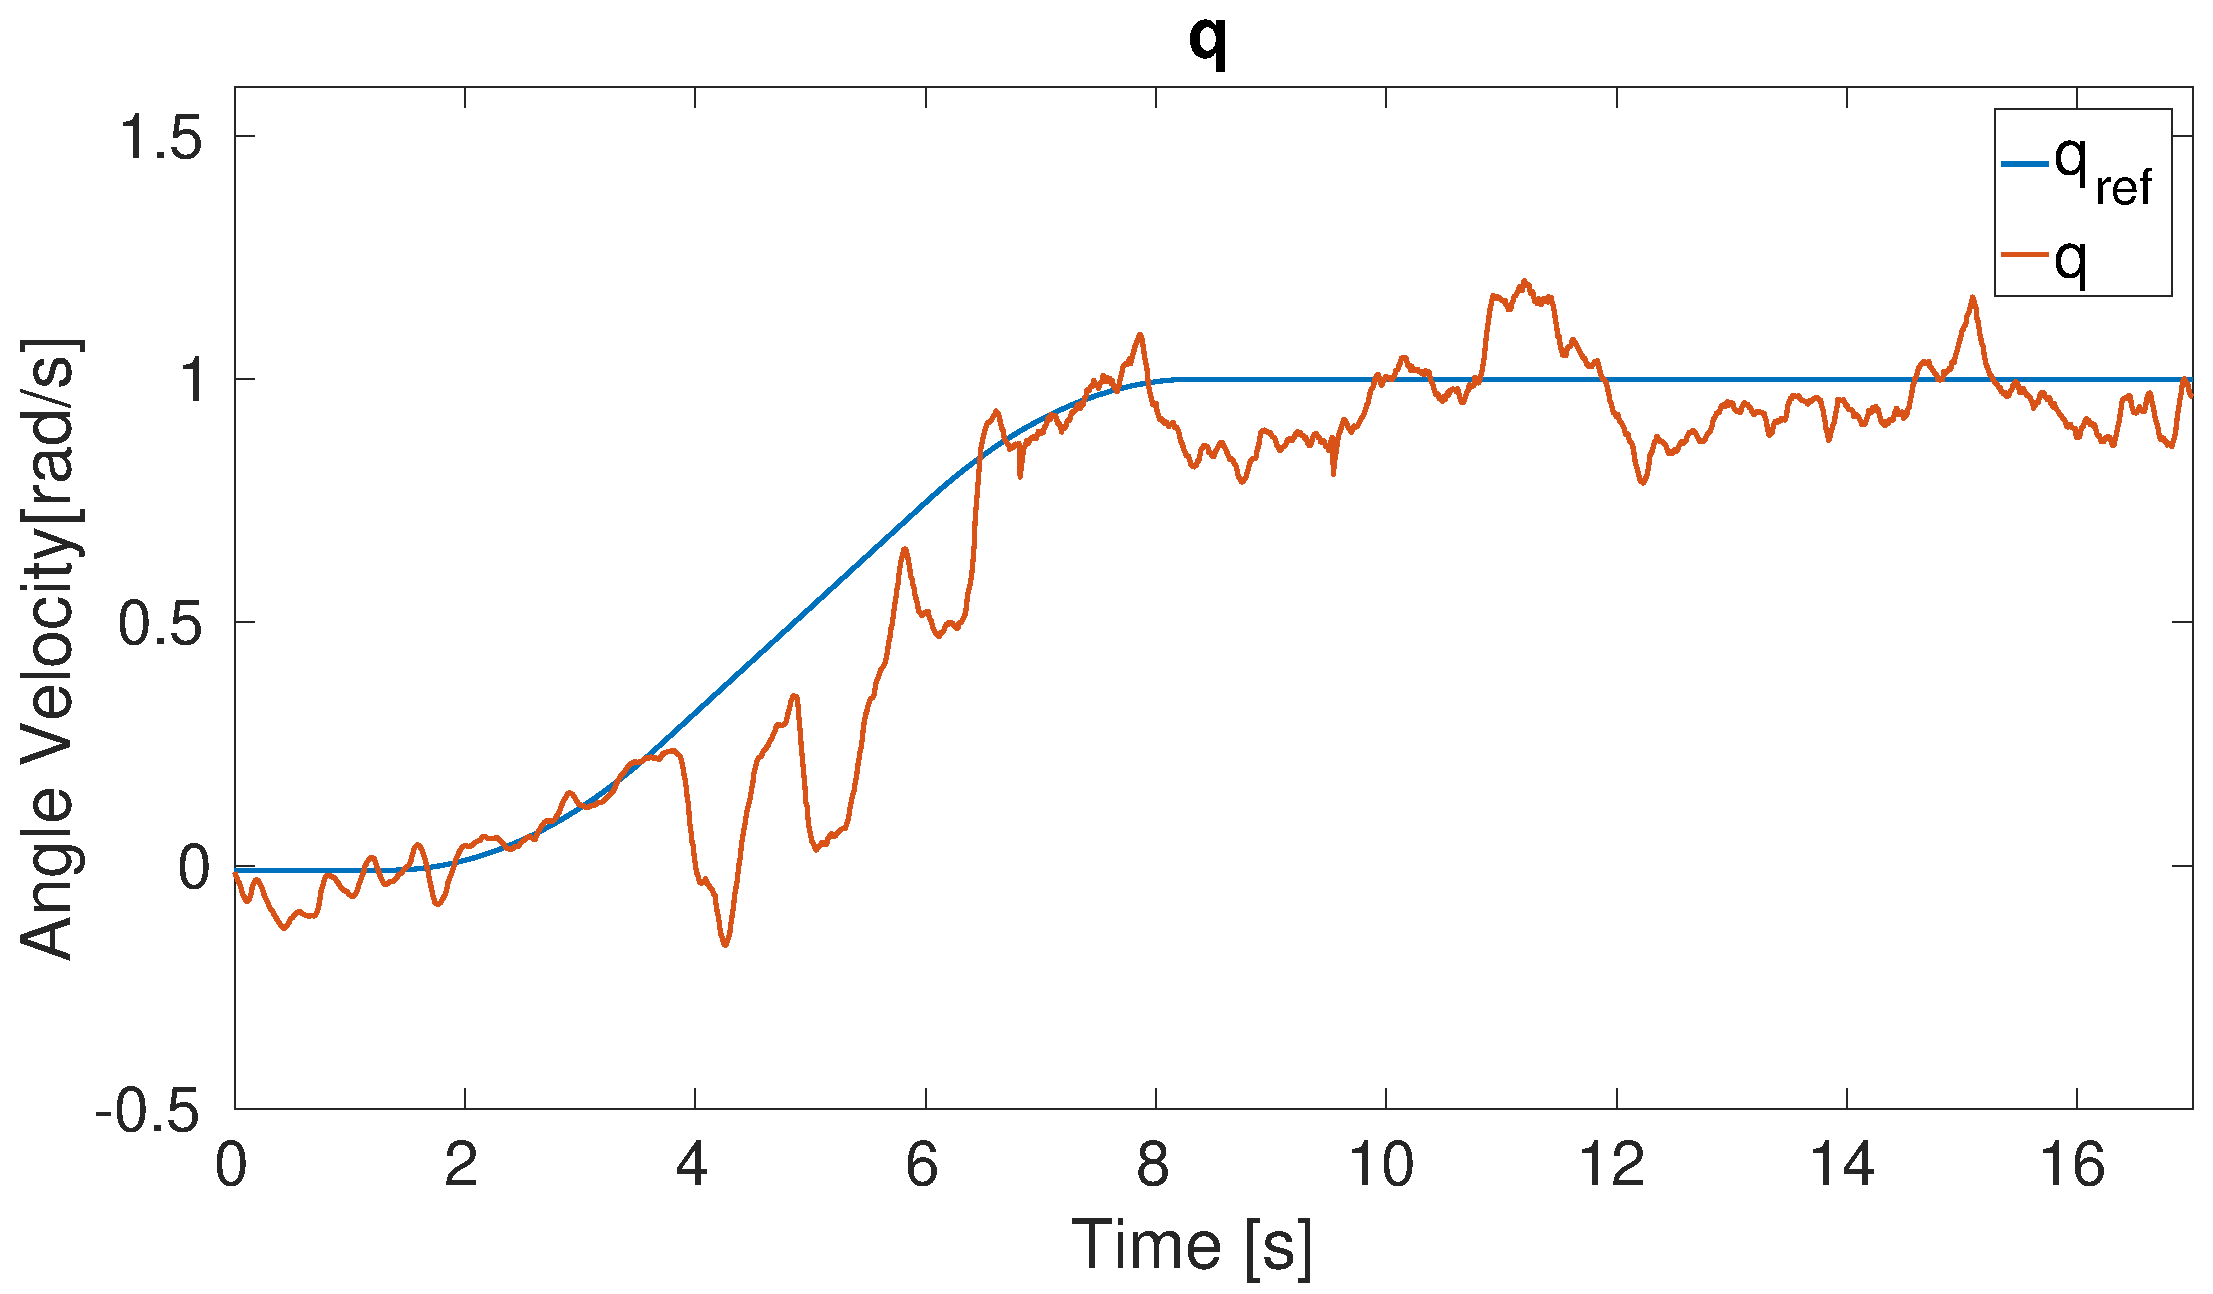
\includegraphics[width=0.4\textwidth]{testStepAllQs3e10a1}}
  \qquad
  \subfloat[][\label{fig:AppsimStepAllQRate} Simulated response in $\pitchVelocity$.]{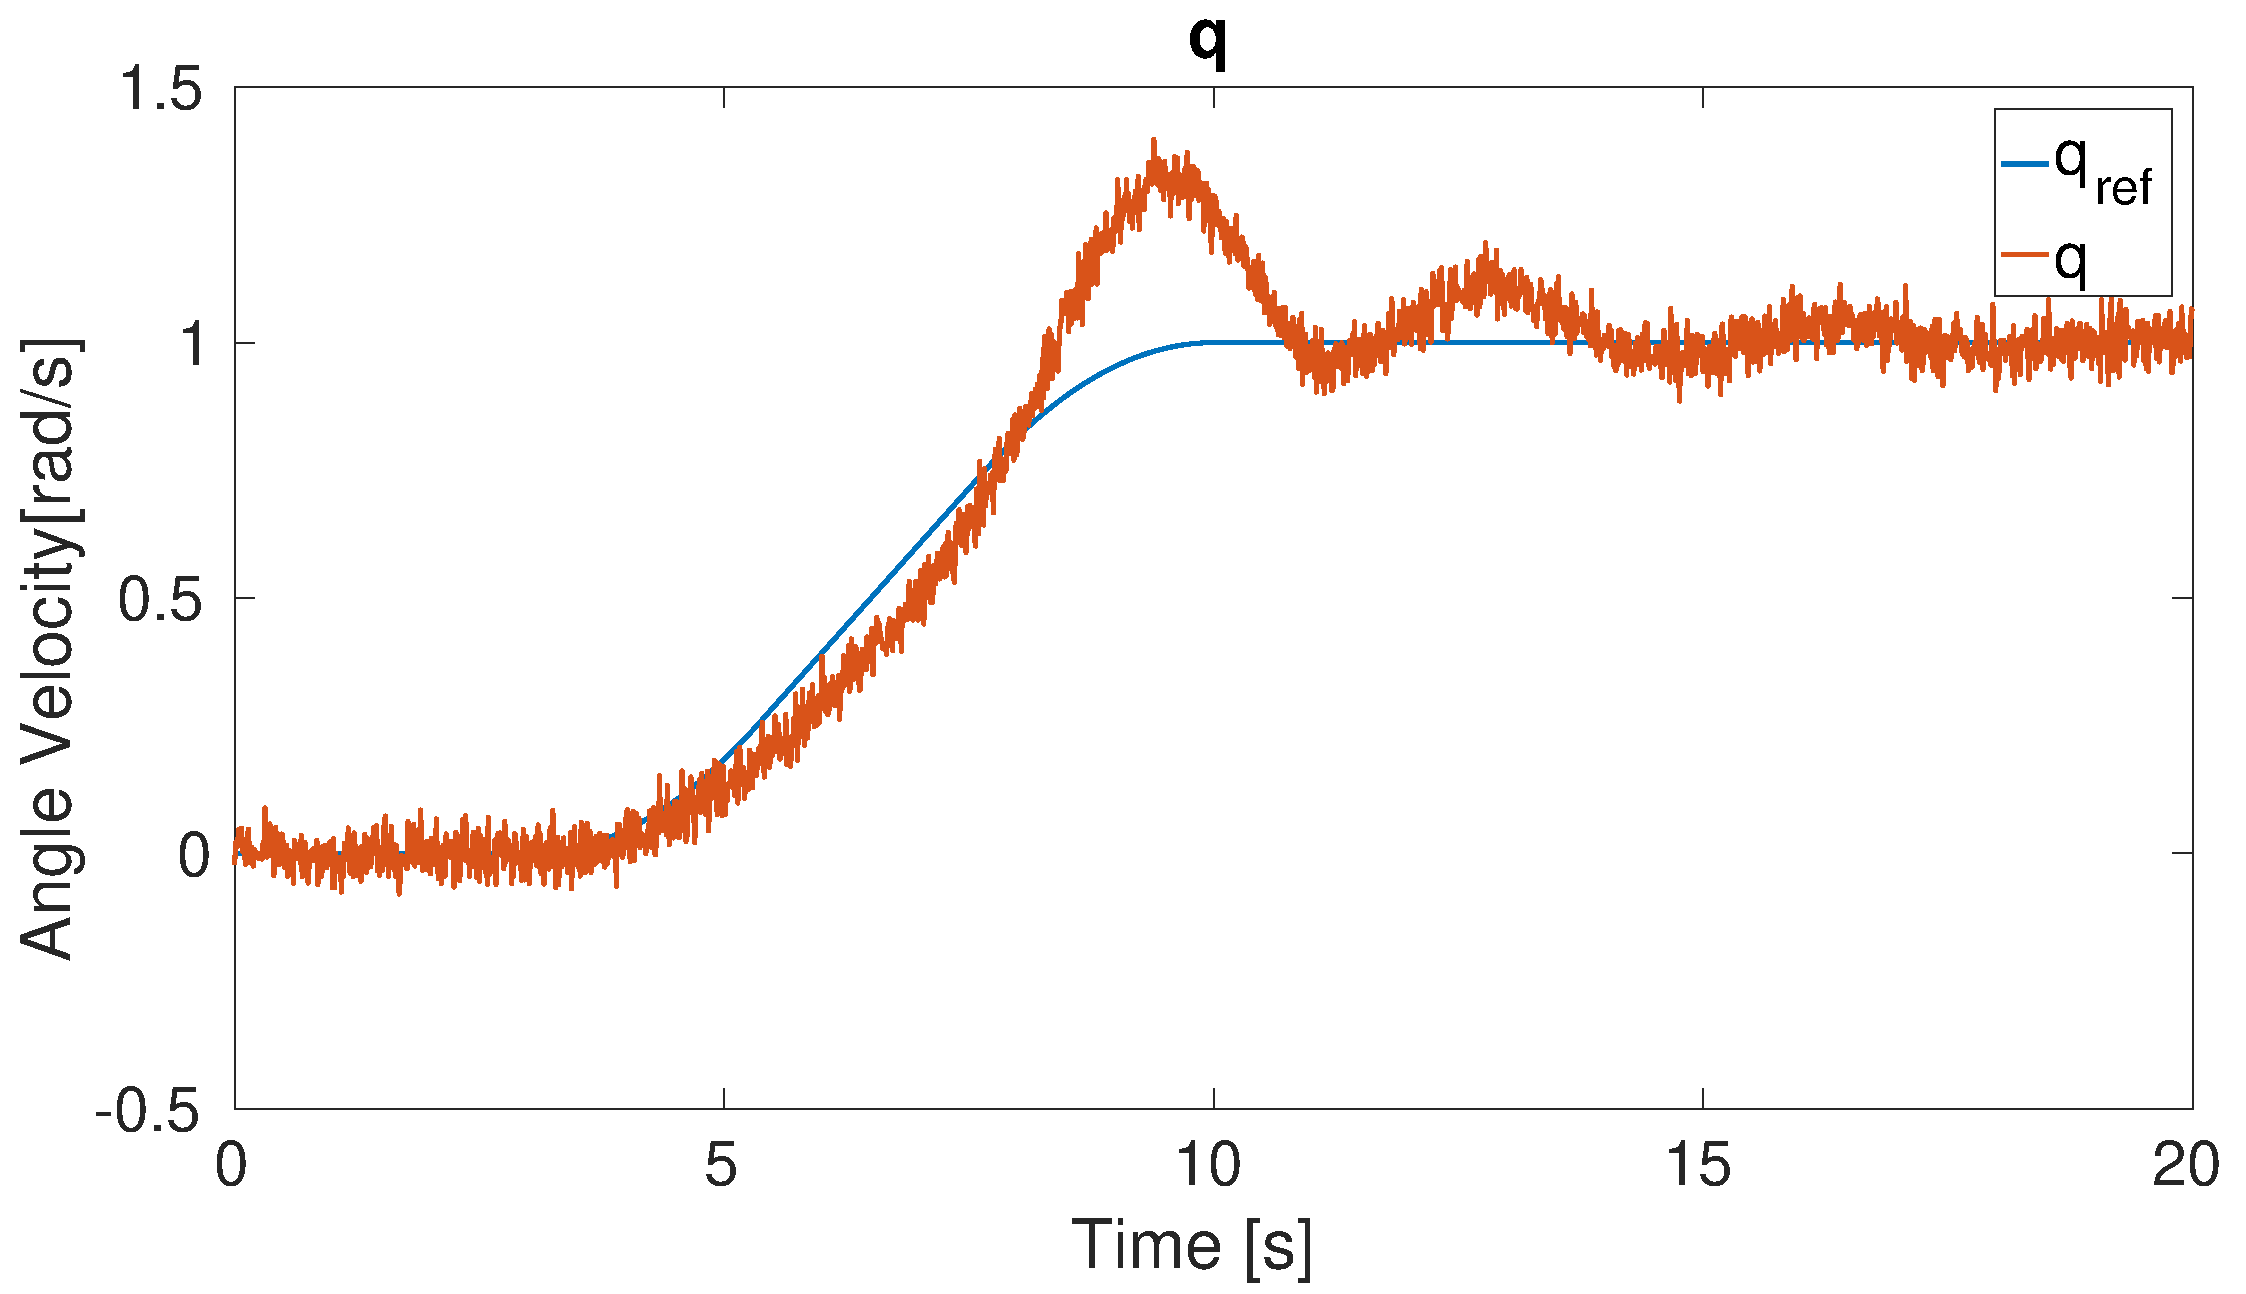
\includegraphics[width=0.4\textwidth]{simStepAllQs3e10a1}}
  \qquad
  \subfloat[][\label{fig:ApptestStepAllRRate} Test response in $\yawVelocity$.]{\includegraphics[width=0.4\textwidth]{testStepAllRs3e10a1}}
  \qquad
  \subfloat[][\label{fig:AppsimStepAllRRate} Simulated response in $\yawVelocity$.]{\includegraphics[width=0.4\textwidth]{simStepAllRs3e10a1}}
  \caption{\label{fig:AppStepAllRate}% 
  A smooth step with $q_{\text{0}} = 0$, $q_{\text{f}} = 1$, $t_{\text{s}} = 3$, $t_{\text{f}} = 15$ and $V = 1.5 (q_{\text{f}} - q_{\text{0}})/(t_{\text{f}} - t_{\text{s}}))$ was applied in all angular velocities at the same time while using the rate controller.}
\end{figure}

\begin{figure}[tbp]
  \centering
  \subfloat[][\label{fig:ApptestSinP} Test response in $\rollVelocity$.]{\includegraphics[width=0.4\textwidth]{testSinPA1}}
  \qquad
  \subfloat[][\label{fig:AppsimSinP} Simulated response in  $\rollVelocity$.]{\includegraphics[width=0.4\textwidth]{simSinPA1}}
  \qquad
  \subfloat[][\label{fig:ApptestSinQ} Test response in $\pitchVelocity$.]{\includegraphics[width=0.4\textwidth]{testSinQA1}}
  \qquad
  \subfloat[][\label{fig:AppsimSinQ} Simulated response in $\pitchVelocity$.]{\includegraphics[width=0.4\textwidth]{simSinQA1}}
  \qquad
  \subfloat[][\label{fig:ApptestSinR} Test response in $\yawVelocity$.]{\includegraphics[width=0.4\textwidth]{testSinRA1}}
  \qquad
  \subfloat[][\label{fig:AppsimSinR} Simulated response in $\yawVelocity$.]{\includegraphics[width=0.4\textwidth]{simSinRA1}}
    \caption{\label{fig:AppSin1Rate}%
   A sine signal with amplitude $1$ and frequency $0.5\ \hertz$ was applied in one angular velocity at a time while using the rate controller. While a sine signal was applied in one angular velocity the other angular velocities were controlled with the reference zero.}
\end{figure}

\begin{figure}
\centering
  \subfloat[][\label{fig:ApptestSinAllPRate} Test response in $\rollVelocity$.]{\includegraphics[width=0.4\textwidth]{testSinAllPA1}}
  \qquad
  \subfloat[][\label{fig:AppsimSinAllPRate} Simulated response in $\rollVelocity$.]{\includegraphics[width=0.4\textwidth]{simSinAllPA1}}
  \qquad
  \subfloat[][\label{fig:ApptestSinAllQRate} Test response in $\pitchVelocity$.]{\includegraphics[width=0.4\textwidth]{testSinAllQA1}}
  \qquad
  \subfloat[][\label{fig:AppsimSinAllQRate} Simulated response in $\pitchVelocity$.]{\includegraphics[width=0.4\textwidth]{simSinAllQA1}}
  \qquad
  \subfloat[][\label{fig:ApptestSinAllRRate} Test response in $\yawVelocity$.]{\includegraphics[width=0.4\textwidth]{testSinAllRA1}}
  \qquad
  \subfloat[][\label{fig:AppsimSinAllRRate} Simulated response in $\yawVelocity$.]{\includegraphics[width=0.4\textwidth]{simSinAllRA1}}
  \caption{\label{fig:AppSinAllRate}%
  A sine signal with amplitude $1$ and frequency $0.5\ \hertz$ was applied in all angular velocities at the same time while using the rate controller.}
\end{figure}


\begin{figure}[tbp]
  \centering
  \subfloat[][\label{fig:ApptestSin05P} Test response in $\rollVelocity$.]{\includegraphics[width=0.4\textwidth]{testSinPA05}}
  \qquad
  \subfloat[][\label{fig:AppsimSin05P} Simulated response in $\rollVelocity$.]{\includegraphics[width=0.4\textwidth]{simSinPA05}}
  \qquad
  \subfloat[][\label{fig:ApptestSin05Q} Test response in $\pitchVelocity$.]{\includegraphics[width=0.4\textwidth]{testSinQA05}}
  \qquad
  \subfloat[][\label{fig:AppsimSin05Q} Simulated response in $\pitchVelocity$.]{\includegraphics[width=0.4\textwidth]{simSinQA05}}
  \qquad
  \subfloat[][\label{fig:ApptestSin05R}  Test response in $\yawVelocity$.]{\includegraphics[width=0.4\textwidth]{testSinRA05}}
  \qquad
  \subfloat[][\label{fig:AppsimSin50R}  Simulated response in $\yawVelocity$.]{\includegraphics[width=0.4\textwidth]{simSinRA05}}
    \caption{\label{fig:AppSin05Rate}%
      A sine signal with amplitude $0.5$ and frequency $0.5\ \hertz$ was applied in one angular velocity at a time while using the rate controller. While a sine signal was applied in one angular velocity the other angular velocities were controlled with the reference zero.}
\end{figure}

\begin{figure}
\centering
  \subfloat[][\label{fig:ApptestSinAll05PRate} Test response in $\rollVelocity$.]{\includegraphics[width=0.4\textwidth]{testSinAllPA05}}
  \qquad
  \subfloat[][\label{fig:AppsimSinAll05PRate} Simulated response in $\rollVelocity$.]{\includegraphics[width=0.4\textwidth]{simSinAllPA05}}
  \qquad
  \subfloat[][\label{fig:AppTestSinAll05QRate} Test response in $\pitchVelocity$.]{\includegraphics[width=0.4\textwidth]{testSinAllQA05}}
  \qquad
  \subfloat[][\label{fig:AppsimSinAll05QRate} Simulated response in $\pitchVelocity$.]{\includegraphics[width=0.4\textwidth]{simSinAllRA05}}
  \qquad
  \subfloat[][\label{fig:AppTestSinAll05RRate} Test response in $\yawVelocity$.]{\includegraphics[width=0.4\textwidth]{testSinAllRA05}}
  \qquad
  \subfloat[][\label{fig:AppsimSinAll05RRate} Simulated response in $\yawVelocity$.]{\includegraphics[width=0.4\textwidth]{simSinAllQA05}}
  \caption{\label{fig:AppSinAll05Rate}%
  Sine signals  with amplitude $0.5$ and frequency $0.5\ \hertz$ were applied in all angular velocities at the same time while using the rate controller.}
\end{figure}

%%%%%%%%%%%%%%%%%%%%%%%%%%%Depth%%%%%%%%%%%%%%%%
\begin{figure}[tbp]
  \centering
  \subfloat[][\label{fig:ApptestStepD1} A smooth step applied in $\zPosition$.]{\includegraphics[width=0.4\textwidth]{testStepDepth3e10a1}}
  \qquad
  \subfloat[][\label{fig:ApptestStepD2} A step applied in $\zPosition$.]{\includegraphics[width=0.4\textwidth]{testConstantD1}}
  \caption{\label{fig:AppStepD}%
    Steps applied to $\zPosition$. A smooth step from $0.4\ \meter$ to $1\ \meter$ is shown in (a) and a step from $0.5 \meter$ to $2 \meter$ is shown in (b).}
\end{figure}